\documentclass[twoside]{book}

% Packages required by doxygen
\usepackage{fixltx2e}
\usepackage{calc}
\usepackage{doxygen}
\usepackage[export]{adjustbox} % also loads graphicx
\usepackage{graphicx}
\usepackage[utf8]{inputenc}
\usepackage{makeidx}
\usepackage{multicol}
\usepackage{multirow}
\PassOptionsToPackage{warn}{textcomp}
\usepackage{textcomp}
\usepackage[nointegrals]{wasysym}
\usepackage[table]{xcolor}

% Font selection
\usepackage[T1]{fontenc}
\usepackage[scaled=.90]{helvet}
\usepackage{courier}
\usepackage{amssymb}
\usepackage{sectsty}
\renewcommand{\familydefault}{\sfdefault}
\allsectionsfont{%
  \fontseries{bc}\selectfont%
  \color{darkgray}%
}
\renewcommand{\DoxyLabelFont}{%
  \fontseries{bc}\selectfont%
  \color{darkgray}%
}
\newcommand{\+}{\discretionary{\mbox{\scriptsize$\hookleftarrow$}}{}{}}

% Page & text layout
\usepackage{geometry}
\geometry{%
  a4paper,%
  top=2.5cm,%
  bottom=2.5cm,%
  left=2.5cm,%
  right=2.5cm%
}
\tolerance=750
\hfuzz=15pt
\hbadness=750
\setlength{\emergencystretch}{15pt}
\setlength{\parindent}{0cm}
\setlength{\parskip}{3ex plus 2ex minus 2ex}
\makeatletter
\renewcommand{\paragraph}{%
  \@startsection{paragraph}{4}{0ex}{-1.0ex}{1.0ex}{%
    \normalfont\normalsize\bfseries\SS@parafont%
  }%
}
\renewcommand{\subparagraph}{%
  \@startsection{subparagraph}{5}{0ex}{-1.0ex}{1.0ex}{%
    \normalfont\normalsize\bfseries\SS@subparafont%
  }%
}
\makeatother

% Headers & footers
\usepackage{fancyhdr}
\pagestyle{fancyplain}
\fancyhead[LE]{\fancyplain{}{\bfseries\thepage}}
\fancyhead[CE]{\fancyplain{}{}}
\fancyhead[RE]{\fancyplain{}{\bfseries\leftmark}}
\fancyhead[LO]{\fancyplain{}{\bfseries\rightmark}}
\fancyhead[CO]{\fancyplain{}{}}
\fancyhead[RO]{\fancyplain{}{\bfseries\thepage}}
\fancyfoot[LE]{\fancyplain{}{}}
\fancyfoot[CE]{\fancyplain{}{}}
\fancyfoot[RE]{\fancyplain{}{\bfseries\scriptsize Generated by Doxygen }}
\fancyfoot[LO]{\fancyplain{}{\bfseries\scriptsize Generated by Doxygen }}
\fancyfoot[CO]{\fancyplain{}{}}
\fancyfoot[RO]{\fancyplain{}{}}
\renewcommand{\footrulewidth}{0.4pt}
\renewcommand{\chaptermark}[1]{%
  \markboth{#1}{}%
}
\renewcommand{\sectionmark}[1]{%
  \markright{\thesection\ #1}%
}

% Indices & bibliography
\usepackage{natbib}
\usepackage[titles]{tocloft}
\setcounter{tocdepth}{3}
\setcounter{secnumdepth}{5}
\makeindex

% Hyperlinks (required, but should be loaded last)
\usepackage{ifpdf}
\ifpdf
  \usepackage[pdftex,pagebackref=true]{hyperref}
\else
  \usepackage[ps2pdf,pagebackref=true]{hyperref}
\fi
\hypersetup{%
  colorlinks=true,%
  linkcolor=blue,%
  citecolor=blue,%
  unicode%
}

% Custom commands
\newcommand{\clearemptydoublepage}{%
  \newpage{\pagestyle{empty}\cleardoublepage}%
}

\usepackage{caption}
\captionsetup{labelsep=space,justification=centering,font={bf},singlelinecheck=off,skip=4pt,position=top}

%===== C O N T E N T S =====

\begin{document}

% Titlepage & ToC
\hypersetup{pageanchor=false,
             bookmarksnumbered=true,
             pdfencoding=unicode
            }
\pagenumbering{alph}
\begin{titlepage}
\vspace*{7cm}
\begin{center}%
{\Large A\+D-\/\+E\+YE \\[1ex]\large 0.\+1 }\\
\vspace*{1cm}
{\large Generated by Doxygen 1.8.13}\\
\end{center}
\end{titlepage}
\clearemptydoublepage
\pagenumbering{roman}
\tableofcontents
\clearemptydoublepage
\pagenumbering{arabic}
\hypersetup{pageanchor=true}

%--- Begin generated contents ---
\chapter{Namespace Index}
\section{Namespace List}
Here is a list of all namespaces with brief descriptions\+:\begin{DoxyCompactList}
\item\contentsline{section}{\hyperlink{namespacecamera__info__publisher}{camera\+\_\+info\+\_\+publisher} }{\pageref{namespacecamera__info__publisher}}{}
\item\contentsline{section}{\hyperlink{namespaceFeatureControl}{Feature\+Control} }{\pageref{namespaceFeatureControl}}{}
\item\contentsline{section}{\hyperlink{namespacegnss__broadcaster}{gnss\+\_\+broadcaster} }{\pageref{namespacegnss__broadcaster}}{}
\item\contentsline{section}{\hyperlink{namespacemanager}{manager} }{\pageref{namespacemanager}}{}
\item\contentsline{section}{\hyperlink{namespacemodifyLaunchTemplate}{modify\+Launch\+Template} }{\pageref{namespacemodifyLaunchTemplate}}{}
\item\contentsline{section}{\hyperlink{namespacepoint__cloud__receiver}{point\+\_\+cloud\+\_\+receiver} }{\pageref{namespacepoint__cloud__receiver}}{}
\item\contentsline{section}{\hyperlink{namespacerp__manager}{rp\+\_\+manager} }{\pageref{namespacerp__manager}}{}
\item\contentsline{section}{\hyperlink{namespacesafetySupervisor}{safety\+Supervisor} }{\pageref{namespacesafetySupervisor}}{}
\item\contentsline{section}{\hyperlink{namespacesender}{sender} }{\pageref{namespacesender}}{}
\item\contentsline{section}{\hyperlink{namespacetracked__objects__adapter}{tracked\+\_\+objects\+\_\+adapter} }{\pageref{namespacetracked__objects__adapter}}{}
\end{DoxyCompactList}

\chapter{Class Index}
\section{Class List}
Here are the classes, structs, unions and interfaces with brief descriptions\+:\begin{DoxyCompactList}
\item\contentsline{section}{\hyperlink{classcameraObjectListFuse}{camera\+Object\+List\+Fuse} }{\pageref{classcameraObjectListFuse}}{}
\item\contentsline{section}{\hyperlink{classCollisionDetector}{Collision\+Detector} \\*A node that detect collision with other objects using the S\+S\+M\+P\+\_\+grid\+Map }{\pageref{classCollisionDetector}}{}
\item\contentsline{section}{\hyperlink{classcontrolSwitch}{control\+Switch} \\*This class is the Switch that selects which channel control the car }{\pageref{classcontrolSwitch}}{}
\item\contentsline{section}{\hyperlink{classFeatureControl_1_1FeatureControl}{Feature\+Control.\+Feature\+Control} \\*This is a class for controlling the starting/stopping of the feature }{\pageref{classFeatureControl_1_1FeatureControl}}{}
\item\contentsline{section}{\hyperlink{classGridMapCreator}{Grid\+Map\+Creator} \\*The \hyperlink{classGridMapCreator}{Grid\+Map\+Creator} maintains a grid map used to know where safe places are }{\pageref{classGridMapCreator}}{}
\item\contentsline{section}{\hyperlink{classlidarRadarFuse}{lidar\+Radar\+Fuse} }{\pageref{classlidarRadarFuse}}{}
\item\contentsline{section}{\hyperlink{classobjectListFuse}{object\+List\+Fuse} }{\pageref{classobjectListFuse}}{}
\item\contentsline{section}{\hyperlink{classobjectsFrameAdapter}{objects\+Frame\+Adapter} }{\pageref{classobjectsFrameAdapter}}{}
\item\contentsline{section}{\hyperlink{classOccMapCreator}{Occ\+Map\+Creator} \\*This class is used to extract data from the Grid\+Map given by the \hyperlink{classGridMapCreator}{Grid\+Map\+Creator} }{\pageref{classOccMapCreator}}{}
\item\contentsline{section}{\hyperlink{structPrescanModel}{Prescan\+Model} }{\pageref{structPrescanModel}}{}
\item\contentsline{section}{\hyperlink{structPrescanObject}{Prescan\+Object} \\*This structure handles data from the Prescan Experiment }{\pageref{structPrescanObject}}{}
\item\contentsline{section}{\hyperlink{classradarBroadcaster}{radar\+Broadcaster} }{\pageref{classradarBroadcaster}}{}
\item\contentsline{section}{\hyperlink{classsafetySupervisor_1_1safetySupervisor}{safety\+Supervisor.\+safety\+Supervisor} \\*This is a class for evaluating the \char`\"{}safety of the Supervisor\char`\"{} }{\pageref{classsafetySupervisor_1_1safetySupervisor}}{}
\item\contentsline{section}{\hyperlink{classSafetySupervisor}{Safety\+Supervisor} \\*The Safety Supervisor supervise the automated driving }{\pageref{classSafetySupervisor}}{}
\item\contentsline{section}{\hyperlink{structVectorMap}{Vector\+Map} \\*This structure handles data from the vector map }{\pageref{structVectorMap}}{}
\end{DoxyCompactList}

\chapter{File Index}
\section{File List}
Here is a list of all files with brief descriptions\+:\begin{DoxyCompactList}
\item\contentsline{section}{/home/akanshu/\+A\+D-\/\+E\+Y\+E\+\_\+\+Core/\+A\+D-\/\+E\+Y\+E/\+R\+O\+S\+\_\+\+Packages/src/\+A\+D-\/\+E\+Y\+E/include/\hyperlink{prescanmodel_8h}{prescanmodel.\+h} }{\pageref{prescanmodel_8h}}{}
\item\contentsline{section}{/home/akanshu/\+A\+D-\/\+E\+Y\+E\+\_\+\+Core/\+A\+D-\/\+E\+Y\+E/\+R\+O\+S\+\_\+\+Packages/src/\+A\+D-\/\+E\+Y\+E/include/\hyperlink{vectormap_8h}{vectormap.\+h} }{\pageref{vectormap_8h}}{}
\item\contentsline{section}{/home/akanshu/\+A\+D-\/\+E\+Y\+E\+\_\+\+Core/\+A\+D-\/\+E\+Y\+E/\+R\+O\+S\+\_\+\+Packages/src/\+A\+D-\/\+E\+Y\+E/src/\hyperlink{camera__info__publisher_8py}{camera\+\_\+info\+\_\+publisher.\+py} }{\pageref{camera__info__publisher_8py}}{}
\item\contentsline{section}{/home/akanshu/\+A\+D-\/\+E\+Y\+E\+\_\+\+Core/\+A\+D-\/\+E\+Y\+E/\+R\+O\+S\+\_\+\+Packages/src/\+A\+D-\/\+E\+Y\+E/src/\hyperlink{cameraObjectListFuse_8cpp}{camera\+Object\+List\+Fuse.\+cpp} }{\pageref{cameraObjectListFuse_8cpp}}{}
\item\contentsline{section}{/home/akanshu/\+A\+D-\/\+E\+Y\+E\+\_\+\+Core/\+A\+D-\/\+E\+Y\+E/\+R\+O\+S\+\_\+\+Packages/src/\+A\+D-\/\+E\+Y\+E/src/\hyperlink{collisionDetector__node_8cpp}{collision\+Detector\+\_\+node.\+cpp} }{\pageref{collisionDetector__node_8cpp}}{}
\item\contentsline{section}{/home/akanshu/\+A\+D-\/\+E\+Y\+E\+\_\+\+Core/\+A\+D-\/\+E\+Y\+E/\+R\+O\+S\+\_\+\+Packages/src/\+A\+D-\/\+E\+Y\+E/src/\hyperlink{controlSwitch__node_8cpp}{control\+Switch\+\_\+node.\+cpp} }{\pageref{controlSwitch__node_8cpp}}{}
\item\contentsline{section}{/home/akanshu/\+A\+D-\/\+E\+Y\+E\+\_\+\+Core/\+A\+D-\/\+E\+Y\+E/\+R\+O\+S\+\_\+\+Packages/src/\+A\+D-\/\+E\+Y\+E/src/\hyperlink{FeatureControl_8py}{Feature\+Control.\+py} }{\pageref{FeatureControl_8py}}{}
\item\contentsline{section}{/home/akanshu/\+A\+D-\/\+E\+Y\+E\+\_\+\+Core/\+A\+D-\/\+E\+Y\+E/\+R\+O\+S\+\_\+\+Packages/src/\+A\+D-\/\+E\+Y\+E/src/\hyperlink{flattening__node_8cpp}{flattening\+\_\+node.\+cpp} }{\pageref{flattening__node_8cpp}}{}
\item\contentsline{section}{/home/akanshu/\+A\+D-\/\+E\+Y\+E\+\_\+\+Core/\+A\+D-\/\+E\+Y\+E/\+R\+O\+S\+\_\+\+Packages/src/\+A\+D-\/\+E\+Y\+E/src/\hyperlink{gnss__broadcaster_8py}{gnss\+\_\+broadcaster.\+py} }{\pageref{gnss__broadcaster_8py}}{}
\item\contentsline{section}{/home/akanshu/\+A\+D-\/\+E\+Y\+E\+\_\+\+Core/\+A\+D-\/\+E\+Y\+E/\+R\+O\+S\+\_\+\+Packages/src/\+A\+D-\/\+E\+Y\+E/src/\hyperlink{GridMapCreator__node_8cpp}{Grid\+Map\+Creator\+\_\+node.\+cpp} }{\pageref{GridMapCreator__node_8cpp}}{}
\item\contentsline{section}{/home/akanshu/\+A\+D-\/\+E\+Y\+E\+\_\+\+Core/\+A\+D-\/\+E\+Y\+E/\+R\+O\+S\+\_\+\+Packages/src/\+A\+D-\/\+E\+Y\+E/src/\hyperlink{lidarRadarFuse_8cpp}{lidar\+Radar\+Fuse.\+cpp} }{\pageref{lidarRadarFuse_8cpp}}{}
\item\contentsline{section}{/home/akanshu/\+A\+D-\/\+E\+Y\+E\+\_\+\+Core/\+A\+D-\/\+E\+Y\+E/\+R\+O\+S\+\_\+\+Packages/src/\+A\+D-\/\+E\+Y\+E/src/\hyperlink{manager_8py}{manager.\+py} }{\pageref{manager_8py}}{}
\item\contentsline{section}{/home/akanshu/\+A\+D-\/\+E\+Y\+E\+\_\+\+Core/\+A\+D-\/\+E\+Y\+E/\+R\+O\+S\+\_\+\+Packages/src/\+A\+D-\/\+E\+Y\+E/src/\hyperlink{modifyLaunchTemplate_8py}{modify\+Launch\+Template.\+py} }{\pageref{modifyLaunchTemplate_8py}}{}
\item\contentsline{section}{/home/akanshu/\+A\+D-\/\+E\+Y\+E\+\_\+\+Core/\+A\+D-\/\+E\+Y\+E/\+R\+O\+S\+\_\+\+Packages/src/\+A\+D-\/\+E\+Y\+E/src/\hyperlink{objectListFuse_8cpp}{object\+List\+Fuse.\+cpp} }{\pageref{objectListFuse_8cpp}}{}
\item\contentsline{section}{/home/akanshu/\+A\+D-\/\+E\+Y\+E\+\_\+\+Core/\+A\+D-\/\+E\+Y\+E/\+R\+O\+S\+\_\+\+Packages/src/\+A\+D-\/\+E\+Y\+E/src/\hyperlink{objectsFrameAdapter_8cpp}{objects\+Frame\+Adapter.\+cpp} }{\pageref{objectsFrameAdapter_8cpp}}{}
\item\contentsline{section}{/home/akanshu/\+A\+D-\/\+E\+Y\+E\+\_\+\+Core/\+A\+D-\/\+E\+Y\+E/\+R\+O\+S\+\_\+\+Packages/src/\+A\+D-\/\+E\+Y\+E/src/\hyperlink{point__cloud__receiver_8py}{point\+\_\+cloud\+\_\+receiver.\+py} }{\pageref{point__cloud__receiver_8py}}{}
\item\contentsline{section}{/home/akanshu/\+A\+D-\/\+E\+Y\+E\+\_\+\+Core/\+A\+D-\/\+E\+Y\+E/\+R\+O\+S\+\_\+\+Packages/src/\+A\+D-\/\+E\+Y\+E/src/\hyperlink{radar__broadcaster_8cpp}{radar\+\_\+broadcaster.\+cpp} }{\pageref{radar__broadcaster_8cpp}}{}
\item\contentsline{section}{/home/akanshu/\+A\+D-\/\+E\+Y\+E\+\_\+\+Core/\+A\+D-\/\+E\+Y\+E/\+R\+O\+S\+\_\+\+Packages/src/\+A\+D-\/\+E\+Y\+E/src/\hyperlink{rp__manager_8py}{rp\+\_\+manager.\+py} }{\pageref{rp__manager_8py}}{}
\item\contentsline{section}{/home/akanshu/\+A\+D-\/\+E\+Y\+E\+\_\+\+Core/\+A\+D-\/\+E\+Y\+E/\+R\+O\+S\+\_\+\+Packages/src/\+A\+D-\/\+E\+Y\+E/src/\hyperlink{safetySupervisor_8cpp}{safety\+Supervisor.\+cpp} }{\pageref{safetySupervisor_8cpp}}{}
\item\contentsline{section}{/home/akanshu/\+A\+D-\/\+E\+Y\+E\+\_\+\+Core/\+A\+D-\/\+E\+Y\+E/\+R\+O\+S\+\_\+\+Packages/src/\+A\+D-\/\+E\+Y\+E/src/\hyperlink{safetySupervisor_8py}{safety\+Supervisor.\+py} }{\pageref{safetySupervisor_8py}}{}
\item\contentsline{section}{/home/akanshu/\+A\+D-\/\+E\+Y\+E\+\_\+\+Core/\+A\+D-\/\+E\+Y\+E/\+R\+O\+S\+\_\+\+Packages/src/\+A\+D-\/\+E\+Y\+E/src/\hyperlink{sender_8py}{sender.\+py} }{\pageref{sender_8py}}{}
\item\contentsline{section}{/home/akanshu/\+A\+D-\/\+E\+Y\+E\+\_\+\+Core/\+A\+D-\/\+E\+Y\+E/\+R\+O\+S\+\_\+\+Packages/src/\+A\+D-\/\+E\+Y\+E/src/\hyperlink{tracked__objects__adapter_8py}{tracked\+\_\+objects\+\_\+adapter.\+py} }{\pageref{tracked__objects__adapter_8py}}{}
\end{DoxyCompactList}

\chapter{Namespace Documentation}
\hypertarget{namespacecamera__info__publisher}{}\section{camera\+\_\+info\+\_\+publisher Namespace Reference}
\label{namespacecamera__info__publisher}\index{camera\+\_\+info\+\_\+publisher@{camera\+\_\+info\+\_\+publisher}}
\subsection*{Variables}
\begin{DoxyCompactItemize}
\item 
\hyperlink{namespacecamera__info__publisher_a2d8ee42f50f0f1a2f44f8287e3d65fde}{msg} = Camera\+Info()
\item 
\hyperlink{namespacecamera__info__publisher_a7f59bda2969259184c03febc1d727bd6}{frame\+\_\+id}
\item 
\hyperlink{namespacecamera__info__publisher_a067a669c555177e826c9b42f9f32fcf3}{height}
\item 
\hyperlink{namespacecamera__info__publisher_a446dc1352be5699a99f9660084e54054}{width}
\item 
\hyperlink{namespacecamera__info__publisher_ab2708da5cf95209018c33acdf374063f}{D}
\item 
\hyperlink{namespacecamera__info__publisher_ae45fa74c6c253f2ebea439d68bdc1fe3}{K}
\item 
\hyperlink{namespacecamera__info__publisher_a9658edfae454ca997cf347704aaa72c3}{R}
\item 
\hyperlink{namespacecamera__info__publisher_a6810e43381f6898ecd0cbedb8a569a7e}{P}
\item 
\hyperlink{namespacecamera__info__publisher_a974733f566916645397703bbee3273d9}{anonymous}
\item 
\hyperlink{namespacecamera__info__publisher_a41969f5fd2d4f608064d7b2d1513450a}{rate} = rospy.\+Rate(10.\+0)
\item 
\hyperlink{namespacecamera__info__publisher_adcc8066d95987066960a2d4861b9a2b9}{pub} = rospy.\+Publisher(sys.\+argv\mbox{[}1\mbox{]}, Camera\+Info, queue\+\_\+size=1)
\end{DoxyCompactItemize}


\subsection{Variable Documentation}
\mbox{\Hypertarget{namespacecamera__info__publisher_a974733f566916645397703bbee3273d9}\label{namespacecamera__info__publisher_a974733f566916645397703bbee3273d9}} 
\index{camera\+\_\+info\+\_\+publisher@{camera\+\_\+info\+\_\+publisher}!anonymous@{anonymous}}
\index{anonymous@{anonymous}!camera\+\_\+info\+\_\+publisher@{camera\+\_\+info\+\_\+publisher}}
\subsubsection{\texorpdfstring{anonymous}{anonymous}}
{\footnotesize\ttfamily camera\+\_\+info\+\_\+publisher.\+anonymous}

\mbox{\Hypertarget{namespacecamera__info__publisher_ab2708da5cf95209018c33acdf374063f}\label{namespacecamera__info__publisher_ab2708da5cf95209018c33acdf374063f}} 
\index{camera\+\_\+info\+\_\+publisher@{camera\+\_\+info\+\_\+publisher}!D@{D}}
\index{D@{D}!camera\+\_\+info\+\_\+publisher@{camera\+\_\+info\+\_\+publisher}}
\subsubsection{\texorpdfstring{D}{D}}
{\footnotesize\ttfamily camera\+\_\+info\+\_\+publisher.\+D}

\mbox{\Hypertarget{namespacecamera__info__publisher_a7f59bda2969259184c03febc1d727bd6}\label{namespacecamera__info__publisher_a7f59bda2969259184c03febc1d727bd6}} 
\index{camera\+\_\+info\+\_\+publisher@{camera\+\_\+info\+\_\+publisher}!frame\+\_\+id@{frame\+\_\+id}}
\index{frame\+\_\+id@{frame\+\_\+id}!camera\+\_\+info\+\_\+publisher@{camera\+\_\+info\+\_\+publisher}}
\subsubsection{\texorpdfstring{frame\+\_\+id}{frame\_id}}
{\footnotesize\ttfamily camera\+\_\+info\+\_\+publisher.\+frame\+\_\+id}

\mbox{\Hypertarget{namespacecamera__info__publisher_a067a669c555177e826c9b42f9f32fcf3}\label{namespacecamera__info__publisher_a067a669c555177e826c9b42f9f32fcf3}} 
\index{camera\+\_\+info\+\_\+publisher@{camera\+\_\+info\+\_\+publisher}!height@{height}}
\index{height@{height}!camera\+\_\+info\+\_\+publisher@{camera\+\_\+info\+\_\+publisher}}
\subsubsection{\texorpdfstring{height}{height}}
{\footnotesize\ttfamily camera\+\_\+info\+\_\+publisher.\+height}

\mbox{\Hypertarget{namespacecamera__info__publisher_ae45fa74c6c253f2ebea439d68bdc1fe3}\label{namespacecamera__info__publisher_ae45fa74c6c253f2ebea439d68bdc1fe3}} 
\index{camera\+\_\+info\+\_\+publisher@{camera\+\_\+info\+\_\+publisher}!K@{K}}
\index{K@{K}!camera\+\_\+info\+\_\+publisher@{camera\+\_\+info\+\_\+publisher}}
\subsubsection{\texorpdfstring{K}{K}}
{\footnotesize\ttfamily camera\+\_\+info\+\_\+publisher.\+K}

\mbox{\Hypertarget{namespacecamera__info__publisher_a2d8ee42f50f0f1a2f44f8287e3d65fde}\label{namespacecamera__info__publisher_a2d8ee42f50f0f1a2f44f8287e3d65fde}} 
\index{camera\+\_\+info\+\_\+publisher@{camera\+\_\+info\+\_\+publisher}!msg@{msg}}
\index{msg@{msg}!camera\+\_\+info\+\_\+publisher@{camera\+\_\+info\+\_\+publisher}}
\subsubsection{\texorpdfstring{msg}{msg}}
{\footnotesize\ttfamily camera\+\_\+info\+\_\+publisher.\+msg = Camera\+Info()}

\mbox{\Hypertarget{namespacecamera__info__publisher_a6810e43381f6898ecd0cbedb8a569a7e}\label{namespacecamera__info__publisher_a6810e43381f6898ecd0cbedb8a569a7e}} 
\index{camera\+\_\+info\+\_\+publisher@{camera\+\_\+info\+\_\+publisher}!P@{P}}
\index{P@{P}!camera\+\_\+info\+\_\+publisher@{camera\+\_\+info\+\_\+publisher}}
\subsubsection{\texorpdfstring{P}{P}}
{\footnotesize\ttfamily camera\+\_\+info\+\_\+publisher.\+P}

\mbox{\Hypertarget{namespacecamera__info__publisher_adcc8066d95987066960a2d4861b9a2b9}\label{namespacecamera__info__publisher_adcc8066d95987066960a2d4861b9a2b9}} 
\index{camera\+\_\+info\+\_\+publisher@{camera\+\_\+info\+\_\+publisher}!pub@{pub}}
\index{pub@{pub}!camera\+\_\+info\+\_\+publisher@{camera\+\_\+info\+\_\+publisher}}
\subsubsection{\texorpdfstring{pub}{pub}}
{\footnotesize\ttfamily camera\+\_\+info\+\_\+publisher.\+pub = rospy.\+Publisher(sys.\+argv\mbox{[}1\mbox{]}, Camera\+Info, queue\+\_\+size=1)}

\mbox{\Hypertarget{namespacecamera__info__publisher_a9658edfae454ca997cf347704aaa72c3}\label{namespacecamera__info__publisher_a9658edfae454ca997cf347704aaa72c3}} 
\index{camera\+\_\+info\+\_\+publisher@{camera\+\_\+info\+\_\+publisher}!R@{R}}
\index{R@{R}!camera\+\_\+info\+\_\+publisher@{camera\+\_\+info\+\_\+publisher}}
\subsubsection{\texorpdfstring{R}{R}}
{\footnotesize\ttfamily camera\+\_\+info\+\_\+publisher.\+R}

\mbox{\Hypertarget{namespacecamera__info__publisher_a41969f5fd2d4f608064d7b2d1513450a}\label{namespacecamera__info__publisher_a41969f5fd2d4f608064d7b2d1513450a}} 
\index{camera\+\_\+info\+\_\+publisher@{camera\+\_\+info\+\_\+publisher}!rate@{rate}}
\index{rate@{rate}!camera\+\_\+info\+\_\+publisher@{camera\+\_\+info\+\_\+publisher}}
\subsubsection{\texorpdfstring{rate}{rate}}
{\footnotesize\ttfamily camera\+\_\+info\+\_\+publisher.\+rate = rospy.\+Rate(10.\+0)}

\mbox{\Hypertarget{namespacecamera__info__publisher_a446dc1352be5699a99f9660084e54054}\label{namespacecamera__info__publisher_a446dc1352be5699a99f9660084e54054}} 
\index{camera\+\_\+info\+\_\+publisher@{camera\+\_\+info\+\_\+publisher}!width@{width}}
\index{width@{width}!camera\+\_\+info\+\_\+publisher@{camera\+\_\+info\+\_\+publisher}}
\subsubsection{\texorpdfstring{width}{width}}
{\footnotesize\ttfamily camera\+\_\+info\+\_\+publisher.\+width}


\hypertarget{namespaceFeatureControl}{}\section{Feature\+Control Namespace Reference}
\label{namespaceFeatureControl}\index{Feature\+Control@{Feature\+Control}}
\subsection*{Classes}
\begin{DoxyCompactItemize}
\item 
class \hyperlink{classFeatureControl_1_1FeatureControl}{Feature\+Control}
\begin{DoxyCompactList}\small\item\em This is a class for controlling the starting/stopping of the feature. \end{DoxyCompactList}\end{DoxyCompactItemize}
\subsection*{Variables}
\begin{DoxyCompactItemize}
\item 
float \hyperlink{namespaceFeatureControl_aeebd4e13e6a3a0dde7d720af530ae36d}{D\+E\+F\+A\+U\+L\+T\+\_\+\+W\+A\+I\+T\+\_\+\+T\+I\+ME} = 0.\+1
\end{DoxyCompactItemize}


\subsection{Variable Documentation}
\mbox{\Hypertarget{namespaceFeatureControl_aeebd4e13e6a3a0dde7d720af530ae36d}\label{namespaceFeatureControl_aeebd4e13e6a3a0dde7d720af530ae36d}} 
\index{Feature\+Control@{Feature\+Control}!D\+E\+F\+A\+U\+L\+T\+\_\+\+W\+A\+I\+T\+\_\+\+T\+I\+ME@{D\+E\+F\+A\+U\+L\+T\+\_\+\+W\+A\+I\+T\+\_\+\+T\+I\+ME}}
\index{D\+E\+F\+A\+U\+L\+T\+\_\+\+W\+A\+I\+T\+\_\+\+T\+I\+ME@{D\+E\+F\+A\+U\+L\+T\+\_\+\+W\+A\+I\+T\+\_\+\+T\+I\+ME}!Feature\+Control@{Feature\+Control}}
\subsubsection{\texorpdfstring{D\+E\+F\+A\+U\+L\+T\+\_\+\+W\+A\+I\+T\+\_\+\+T\+I\+ME}{DEFAULT\_WAIT\_TIME}}
{\footnotesize\ttfamily float Feature\+Control.\+D\+E\+F\+A\+U\+L\+T\+\_\+\+W\+A\+I\+T\+\_\+\+T\+I\+ME = 0.\+1}


\hypertarget{namespacegnss__broadcaster}{}\section{gnss\+\_\+broadcaster Namespace Reference}
\label{namespacegnss__broadcaster}\index{gnss\+\_\+broadcaster@{gnss\+\_\+broadcaster}}
\subsection*{Functions}
\begin{DoxyCompactItemize}
\item 
def \hyperlink{namespacegnss__broadcaster_a0476bd17f38f4829ece1fde1e939ace2}{mycallback} (data)
\end{DoxyCompactItemize}


\subsection{Function Documentation}
\mbox{\Hypertarget{namespacegnss__broadcaster_a0476bd17f38f4829ece1fde1e939ace2}\label{namespacegnss__broadcaster_a0476bd17f38f4829ece1fde1e939ace2}} 
\index{gnss\+\_\+broadcaster@{gnss\+\_\+broadcaster}!mycallback@{mycallback}}
\index{mycallback@{mycallback}!gnss\+\_\+broadcaster@{gnss\+\_\+broadcaster}}
\subsubsection{\texorpdfstring{mycallback()}{mycallback()}}
{\footnotesize\ttfamily def gnss\+\_\+broadcaster.\+mycallback (\begin{DoxyParamCaption}\item[{}]{data }\end{DoxyParamCaption})}


\hypertarget{namespacemanager}{}\section{manager Namespace Reference}
\label{namespacemanager}\index{manager@{manager}}
\subsection*{Functions}
\begin{DoxyCompactItemize}
\item 
def \hyperlink{namespacemanager_ae7c336047eda26124f4453e77f436139}{simulink\+\_\+state\+\_\+callback} (msg)
\begin{DoxyCompactList}\small\item\em The callback function of the subscriped topic /\+Simulink\+\_\+state. \end{DoxyCompactList}\end{DoxyCompactItemize}
\subsection*{Variables}
\begin{DoxyCompactItemize}
\item 
int \hyperlink{namespacemanager_ad92224ba3bccfba54f5d53ee9e9f0e06}{E\+N\+A\+B\+L\+ED} = 1
\item 
int \hyperlink{namespacemanager_acc1a242f79d4757ccec1eafa25991b69}{D\+I\+S\+A\+B\+L\+ED} = 0
\item 
list \hyperlink{namespacemanager_a140ec9bdd4f59ede61032dec9dbd20e3}{F\+E\+A\+T\+U\+R\+E\+\_\+\+E\+N\+A\+B\+L\+ED} = \mbox{[}True for i in range(9)\mbox{]}
\item 
int \hyperlink{namespacemanager_a00b72dc43f7bcfd7f320277e59b9d565}{R\+V\+IZ} = 1
\item 
int \hyperlink{namespacemanager_a0246d765371fcedd6b0c05ee3e97c3ad}{M\+A\+P\+P\+I\+NG} = 2
\item 
int \hyperlink{namespacemanager_a716836983d025722ec1a015848efec7f}{L\+O\+C\+A\+L\+I\+Z\+A\+T\+I\+ON} = 3
\item 
int \hyperlink{namespacemanager_a07571ba2de9edb4dae0269f01bc691cc}{S\+E\+N\+S\+I\+NG} = 4
\item 
int \hyperlink{namespacemanager_a341e1745be0eb2382da0ea818411441c}{D\+E\+T\+E\+C\+T\+I\+ON} = 5
\item 
int \hyperlink{namespacemanager_a2dfd2e80a686fee05e1ade0e51fa5eee}{S\+W\+I\+T\+CH} = 6
\item 
int \hyperlink{namespacemanager_aa7776000dd1f368ae9e4672273662506}{M\+I\+S\+S\+I\+O\+N\+\_\+\+P\+L\+A\+N\+N\+I\+NG} = 7
\item 
int \hyperlink{namespacemanager_a6e5eb6ddb9305d2a2e9bafc6cf3a29b9}{M\+O\+T\+I\+O\+N\+\_\+\+P\+L\+A\+N\+N\+I\+NG} = 8
\item 
int \hyperlink{namespacemanager_a7c64b0011b346aa00685017ed03a6b72}{S\+S\+MP} = 9
\item 
\hyperlink{namespacemanager_af079b1840e898a44e8a8794f632c6747}{rospack} = rospkg.\+Ros\+Pack()
\item 
string \hyperlink{namespacemanager_a6b9923a9dbb3360028e139c3391d3a26}{A\+D\+E\+Y\+E\+\_\+\+P\+A\+C\+K\+A\+G\+E\+\_\+\+L\+O\+C\+A\+T\+I\+ON} = rospack.\+get\+\_\+path(\textquotesingle{}adeye\textquotesingle{})+\char`\"{}/\char`\"{}
\item 
string \hyperlink{namespacemanager_aade405cb0881d91b45085d7bc0f392fa}{L\+A\+U\+N\+C\+H\+\_\+\+F\+O\+L\+D\+E\+R\+\_\+\+L\+O\+C\+A\+T\+I\+ON} = \char`\"{}launch/\char`\"{}
\item 
string \hyperlink{namespacemanager_af8103724e7745859a07a898ea00a8dd0}{R\+V\+I\+Z\+\_\+\+L\+A\+U\+N\+C\+H\+\_\+\+F\+I\+L\+E\+\_\+\+N\+A\+ME} = \char`\"{}my\+\_\+rviz.\+launch\char`\"{}
\item 
string \hyperlink{namespacemanager_ad33e0681d727d6ce2212b3b1e8df8c58}{M\+A\+P\+P\+I\+N\+G\+\_\+\+L\+A\+U\+N\+C\+H\+\_\+\+F\+I\+L\+E\+\_\+\+N\+A\+ME} = \char`\"{}my\+\_\+map.\+launch\char`\"{}
\item 
string \hyperlink{namespacemanager_ac5cea2f52fdf5b97671e86476298f965}{L\+O\+C\+A\+L\+I\+Z\+A\+T\+I\+O\+N\+\_\+\+L\+A\+U\+N\+C\+H\+\_\+\+F\+I\+L\+E\+\_\+\+N\+A\+ME} = \char`\"{}my\+\_\+localization.\+launch\char`\"{}
\item 
string \hyperlink{namespacemanager_a4d3eb6177218a24979c6889f9c1908d2}{F\+A\+K\+E\+\_\+\+L\+O\+C\+A\+L\+I\+Z\+A\+T\+I\+O\+N\+\_\+\+L\+A\+U\+N\+C\+H\+\_\+\+F\+I\+L\+E\+\_\+\+N\+A\+ME} = \char`\"{}my\+\_\+fake\+\_\+localization.\+launch\char`\"{}
\item 
string \hyperlink{namespacemanager_a368d806bbf5be8e72604353b971871d5}{S\+E\+N\+S\+I\+N\+G\+\_\+\+L\+A\+U\+N\+C\+H\+\_\+\+F\+I\+L\+E\+\_\+\+N\+A\+ME} = \char`\"{}my\+\_\+sensing.\+launch\char`\"{}
\item 
string \hyperlink{namespacemanager_a1312c3fc2b915604378de82f841606b3}{D\+E\+T\+E\+C\+T\+I\+O\+N\+\_\+\+L\+A\+U\+N\+C\+H\+\_\+\+F\+I\+L\+E\+\_\+\+N\+A\+ME} = \char`\"{}my\+\_\+detection.\+launch\char`\"{}
\item 
string \hyperlink{namespacemanager_ac734eeabc7266313bdf84d100e8c5d77}{S\+W\+I\+T\+C\+H\+\_\+\+L\+A\+U\+N\+C\+H\+\_\+\+F\+I\+L\+E\+\_\+\+N\+A\+ME} = \char`\"{}switch.\+launch\char`\"{}
\item 
string \hyperlink{namespacemanager_ab7fc10389616b920dfa8634166a53e72}{M\+I\+S\+S\+I\+O\+N\+\_\+\+P\+L\+A\+N\+N\+I\+N\+G\+\_\+\+L\+A\+U\+N\+C\+H\+\_\+\+F\+I\+L\+E\+\_\+\+N\+A\+ME} = \char`\"{}my\+\_\+mission\+\_\+planning.\+launch\char`\"{}
\item 
string \hyperlink{namespacemanager_a60e86ba9ca513ac1fdda1ffd0d08c900}{M\+O\+T\+I\+O\+N\+\_\+\+P\+L\+A\+N\+N\+I\+N\+G\+\_\+\+L\+A\+U\+N\+C\+H\+\_\+\+F\+I\+L\+E\+\_\+\+N\+A\+ME} = \char`\"{}my\+\_\+motion\+\_\+planning.\+launch\char`\"{}
\item 
string \hyperlink{namespacemanager_a48b997992b3e5973e9ccfe2ce7869790}{S\+S\+M\+P\+\_\+\+L\+A\+U\+N\+C\+H\+\_\+\+F\+I\+L\+E\+\_\+\+N\+A\+ME} = \char`\"{}S\+S\+M\+P.\+launch\char`\"{}
\item 
tuple \hyperlink{namespacemanager_abec52dfb99cc7cf63fc7c9c112413570}{R\+V\+I\+Z\+\_\+\+F\+U\+L\+L\+\_\+\+P\+A\+TH} = (\char`\"{}\%s\%s\%s\char`\"{} \% (A\+D\+E\+Y\+E\+\_\+\+P\+A\+C\+K\+A\+G\+E\+\_\+\+L\+O\+C\+A\+T\+I\+ON, \hyperlink{namespacemanager_aade405cb0881d91b45085d7bc0f392fa}{L\+A\+U\+N\+C\+H\+\_\+\+F\+O\+L\+D\+E\+R\+\_\+\+L\+O\+C\+A\+T\+I\+ON}, \hyperlink{namespacemanager_af8103724e7745859a07a898ea00a8dd0}{R\+V\+I\+Z\+\_\+\+L\+A\+U\+N\+C\+H\+\_\+\+F\+I\+L\+E\+\_\+\+N\+A\+ME}))
\item 
tuple \hyperlink{namespacemanager_aa62d8709423fedec1c58eb802a65cd4d}{M\+A\+P\+P\+I\+N\+G\+\_\+\+F\+U\+L\+L\+\_\+\+P\+A\+TH} = (\char`\"{}\%s\%s\%s\char`\"{} \% (A\+D\+E\+Y\+E\+\_\+\+P\+A\+C\+K\+A\+G\+E\+\_\+\+L\+O\+C\+A\+T\+I\+ON, \hyperlink{namespacemanager_aade405cb0881d91b45085d7bc0f392fa}{L\+A\+U\+N\+C\+H\+\_\+\+F\+O\+L\+D\+E\+R\+\_\+\+L\+O\+C\+A\+T\+I\+ON}, \hyperlink{namespacemanager_ad33e0681d727d6ce2212b3b1e8df8c58}{M\+A\+P\+P\+I\+N\+G\+\_\+\+L\+A\+U\+N\+C\+H\+\_\+\+F\+I\+L\+E\+\_\+\+N\+A\+ME}))
\item 
tuple \hyperlink{namespacemanager_a066d10c0cbeebfc5036425b22d06aa6a}{L\+O\+C\+A\+L\+I\+Z\+A\+T\+I\+O\+N\+\_\+\+F\+U\+L\+L\+\_\+\+P\+A\+TH} = (\char`\"{}\%s\%s\%s\char`\"{} \% (A\+D\+E\+Y\+E\+\_\+\+P\+A\+C\+K\+A\+G\+E\+\_\+\+L\+O\+C\+A\+T\+I\+ON, \hyperlink{namespacemanager_aade405cb0881d91b45085d7bc0f392fa}{L\+A\+U\+N\+C\+H\+\_\+\+F\+O\+L\+D\+E\+R\+\_\+\+L\+O\+C\+A\+T\+I\+ON}, \hyperlink{namespacemanager_ac5cea2f52fdf5b97671e86476298f965}{L\+O\+C\+A\+L\+I\+Z\+A\+T\+I\+O\+N\+\_\+\+L\+A\+U\+N\+C\+H\+\_\+\+F\+I\+L\+E\+\_\+\+N\+A\+ME}))
\item 
tuple \hyperlink{namespacemanager_a3f4276e287ba46746f54f0caa40e408d}{F\+A\+K\+E\+\_\+\+L\+O\+C\+A\+L\+I\+Z\+A\+T\+I\+O\+N\+\_\+\+F\+U\+L\+L\+\_\+\+P\+A\+TH} = (\char`\"{}\%s\%s\%s\char`\"{} \% (A\+D\+E\+Y\+E\+\_\+\+P\+A\+C\+K\+A\+G\+E\+\_\+\+L\+O\+C\+A\+T\+I\+ON, \hyperlink{namespacemanager_aade405cb0881d91b45085d7bc0f392fa}{L\+A\+U\+N\+C\+H\+\_\+\+F\+O\+L\+D\+E\+R\+\_\+\+L\+O\+C\+A\+T\+I\+ON}, \hyperlink{namespacemanager_a4d3eb6177218a24979c6889f9c1908d2}{F\+A\+K\+E\+\_\+\+L\+O\+C\+A\+L\+I\+Z\+A\+T\+I\+O\+N\+\_\+\+L\+A\+U\+N\+C\+H\+\_\+\+F\+I\+L\+E\+\_\+\+N\+A\+ME}))
\item 
tuple \hyperlink{namespacemanager_aeedd72a434a67d10fd373ddd152ae332}{S\+E\+N\+S\+I\+N\+G\+\_\+\+F\+U\+L\+L\+\_\+\+P\+A\+TH} = (\char`\"{}\%s\%s\%s\char`\"{} \% (A\+D\+E\+Y\+E\+\_\+\+P\+A\+C\+K\+A\+G\+E\+\_\+\+L\+O\+C\+A\+T\+I\+ON, \hyperlink{namespacemanager_aade405cb0881d91b45085d7bc0f392fa}{L\+A\+U\+N\+C\+H\+\_\+\+F\+O\+L\+D\+E\+R\+\_\+\+L\+O\+C\+A\+T\+I\+ON}, \hyperlink{namespacemanager_a368d806bbf5be8e72604353b971871d5}{S\+E\+N\+S\+I\+N\+G\+\_\+\+L\+A\+U\+N\+C\+H\+\_\+\+F\+I\+L\+E\+\_\+\+N\+A\+ME}))
\item 
tuple \hyperlink{namespacemanager_a6c770a978c4d514742b18d200aa5e09e}{D\+E\+T\+E\+C\+T\+I\+O\+N\+\_\+\+F\+U\+L\+L\+\_\+\+P\+A\+TH} = (\char`\"{}\%s\%s\%s\char`\"{} \% (A\+D\+E\+Y\+E\+\_\+\+P\+A\+C\+K\+A\+G\+E\+\_\+\+L\+O\+C\+A\+T\+I\+ON, \hyperlink{namespacemanager_aade405cb0881d91b45085d7bc0f392fa}{L\+A\+U\+N\+C\+H\+\_\+\+F\+O\+L\+D\+E\+R\+\_\+\+L\+O\+C\+A\+T\+I\+ON}, \hyperlink{namespacemanager_a1312c3fc2b915604378de82f841606b3}{D\+E\+T\+E\+C\+T\+I\+O\+N\+\_\+\+L\+A\+U\+N\+C\+H\+\_\+\+F\+I\+L\+E\+\_\+\+N\+A\+ME}))
\item 
tuple \hyperlink{namespacemanager_aa8c7bc9defad2d982a87f67d530919bc}{S\+W\+I\+T\+C\+H\+\_\+\+F\+U\+L\+L\+\_\+\+P\+A\+TH} = (\char`\"{}\%s\%s\%s\char`\"{} \% (A\+D\+E\+Y\+E\+\_\+\+P\+A\+C\+K\+A\+G\+E\+\_\+\+L\+O\+C\+A\+T\+I\+ON, \hyperlink{namespacemanager_aade405cb0881d91b45085d7bc0f392fa}{L\+A\+U\+N\+C\+H\+\_\+\+F\+O\+L\+D\+E\+R\+\_\+\+L\+O\+C\+A\+T\+I\+ON}, \hyperlink{namespacemanager_ac734eeabc7266313bdf84d100e8c5d77}{S\+W\+I\+T\+C\+H\+\_\+\+L\+A\+U\+N\+C\+H\+\_\+\+F\+I\+L\+E\+\_\+\+N\+A\+ME}))
\item 
tuple \hyperlink{namespacemanager_a3d3b5c1e3f4aa2f976afd6696fb753dc}{M\+I\+S\+S\+I\+O\+N\+\_\+\+P\+L\+A\+N\+N\+I\+N\+G\+\_\+\+F\+U\+L\+L\+\_\+\+P\+A\+TH}
\item 
tuple \hyperlink{namespacemanager_a53957d71bc1b0299a6de2499348c0c7b}{M\+O\+T\+I\+O\+N\+\_\+\+P\+L\+A\+N\+N\+I\+N\+G\+\_\+\+F\+U\+L\+L\+\_\+\+P\+A\+TH}
\item 
tuple \hyperlink{namespacemanager_af8b394f3a0664a2eb78bb3c7ec36dd97}{S\+S\+M\+P\+\_\+\+F\+U\+L\+L\+\_\+\+P\+A\+TH} = (\char`\"{}\%s\%s\%s\char`\"{} \% (A\+D\+E\+Y\+E\+\_\+\+P\+A\+C\+K\+A\+G\+E\+\_\+\+L\+O\+C\+A\+T\+I\+ON, \hyperlink{namespacemanager_aade405cb0881d91b45085d7bc0f392fa}{L\+A\+U\+N\+C\+H\+\_\+\+F\+O\+L\+D\+E\+R\+\_\+\+L\+O\+C\+A\+T\+I\+ON}, \hyperlink{namespacemanager_a48b997992b3e5973e9ccfe2ce7869790}{S\+S\+M\+P\+\_\+\+L\+A\+U\+N\+C\+H\+\_\+\+F\+I\+L\+E\+\_\+\+N\+A\+ME}))
\item 
int \hyperlink{namespacemanager_a114c53938453b5bea9a1d87feb0b8787}{M\+A\+P\+P\+I\+N\+G\+\_\+\+S\+T\+A\+R\+T\+\_\+\+W\+A\+I\+T\+\_\+\+T\+I\+ME} = 10
\item 
int \hyperlink{namespacemanager_a8bb090193ee690460b2d5da5d95d670a}{L\+O\+C\+A\+L\+I\+Z\+A\+T\+I\+O\+N\+\_\+\+S\+T\+A\+R\+T\+\_\+\+W\+A\+I\+T\+\_\+\+T\+I\+ME} = 10
\item 
int \hyperlink{namespacemanager_a8532d59e6a018744dbd2db6ffa66b1e1}{L\+O\+C\+A\+L\+I\+Z\+A\+T\+I\+O\+N\+\_\+\+S\+T\+O\+P\+\_\+\+W\+A\+I\+T\+\_\+\+T\+I\+ME} = 10
\item 
int \hyperlink{namespacemanager_a38f231e60cb3e2fa5c7a738460ddad61}{D\+E\+T\+E\+C\+T\+I\+O\+N\+\_\+\+S\+T\+O\+P\+\_\+\+W\+A\+I\+T\+\_\+\+T\+I\+ME} = 10
\item 
int \hyperlink{namespacemanager_a575cc129790b379cc97a6a24bf765f92}{M\+I\+S\+S\+I\+O\+N\+\_\+\+P\+L\+A\+N\+N\+I\+N\+G\+\_\+\+S\+T\+A\+R\+T\+\_\+\+W\+A\+I\+T\+\_\+\+T\+I\+ME} = 5
\item 
int \hyperlink{namespacemanager_a26d58788b212bc74577124e9ebd27801}{M\+I\+S\+S\+I\+O\+N\+\_\+\+P\+L\+A\+N\+N\+I\+N\+G\+\_\+\+S\+T\+O\+P\+\_\+\+W\+A\+I\+T\+\_\+\+T\+I\+ME} = 10
\item 
int \hyperlink{namespacemanager_ad7506a085f025fae99014ec616f7af1a}{M\+O\+T\+I\+O\+N\+\_\+\+P\+L\+A\+N\+N\+I\+N\+G\+\_\+\+S\+T\+O\+P\+\_\+\+W\+A\+I\+T\+\_\+\+T\+I\+ME} = 10
\item 
list \hyperlink{namespacemanager_af1c387f91036250d99a08f76b85353e3}{previous\+\_\+simulink\+\_\+state} = \mbox{[}\hyperlink{namespacemanager_acc1a242f79d4757ccec1eafa25991b69}{D\+I\+S\+A\+B\+L\+ED}, \hyperlink{namespacemanager_acc1a242f79d4757ccec1eafa25991b69}{D\+I\+S\+A\+B\+L\+ED}, \hyperlink{namespacemanager_acc1a242f79d4757ccec1eafa25991b69}{D\+I\+S\+A\+B\+L\+ED}, \hyperlink{namespacemanager_acc1a242f79d4757ccec1eafa25991b69}{D\+I\+S\+A\+B\+L\+ED}, \hyperlink{namespacemanager_acc1a242f79d4757ccec1eafa25991b69}{D\+I\+S\+A\+B\+L\+ED}, \hyperlink{namespacemanager_acc1a242f79d4757ccec1eafa25991b69}{D\+I\+S\+A\+B\+L\+ED}, \hyperlink{namespacemanager_acc1a242f79d4757ccec1eafa25991b69}{D\+I\+S\+A\+B\+L\+ED}, \hyperlink{namespacemanager_acc1a242f79d4757ccec1eafa25991b69}{D\+I\+S\+A\+B\+L\+ED}, \hyperlink{namespacemanager_acc1a242f79d4757ccec1eafa25991b69}{D\+I\+S\+A\+B\+L\+ED}, \hyperlink{namespacemanager_acc1a242f79d4757ccec1eafa25991b69}{D\+I\+S\+A\+B\+L\+ED}\mbox{]}
\item 
list \hyperlink{namespacemanager_afe07b109c9d2316eff7e41a3e38d2859}{current\+\_\+simulink\+\_\+state} = \mbox{[}\hyperlink{namespacemanager_acc1a242f79d4757ccec1eafa25991b69}{D\+I\+S\+A\+B\+L\+ED}, \hyperlink{namespacemanager_acc1a242f79d4757ccec1eafa25991b69}{D\+I\+S\+A\+B\+L\+ED}, \hyperlink{namespacemanager_acc1a242f79d4757ccec1eafa25991b69}{D\+I\+S\+A\+B\+L\+ED}, \hyperlink{namespacemanager_acc1a242f79d4757ccec1eafa25991b69}{D\+I\+S\+A\+B\+L\+ED}, \hyperlink{namespacemanager_acc1a242f79d4757ccec1eafa25991b69}{D\+I\+S\+A\+B\+L\+ED}, \hyperlink{namespacemanager_acc1a242f79d4757ccec1eafa25991b69}{D\+I\+S\+A\+B\+L\+ED}, \hyperlink{namespacemanager_acc1a242f79d4757ccec1eafa25991b69}{D\+I\+S\+A\+B\+L\+ED}, \hyperlink{namespacemanager_acc1a242f79d4757ccec1eafa25991b69}{D\+I\+S\+A\+B\+L\+ED}, \hyperlink{namespacemanager_acc1a242f79d4757ccec1eafa25991b69}{D\+I\+S\+A\+B\+L\+ED}, \hyperlink{namespacemanager_acc1a242f79d4757ccec1eafa25991b69}{D\+I\+S\+A\+B\+L\+ED}\mbox{]}
\item 
bool \hyperlink{namespacemanager_a182c499b086b54bc448d101234319226}{point\+\_\+map\+\_\+ready} = False
\item 
\hyperlink{namespacemanager_a2a89527ffbd1f9fa4d65bc9ed9ebf834}{Rviz} = \hyperlink{classFeatureControl_1_1FeatureControl}{Feature\+Control}(\hyperlink{namespacemanager_abec52dfb99cc7cf63fc7c9c112413570}{R\+V\+I\+Z\+\_\+\+F\+U\+L\+L\+\_\+\+P\+A\+TH}, \char`\"{}Rviz\char`\"{})
\item 
\hyperlink{namespacemanager_af454674dd3d624772b2de2685f10c88c}{Mapping} = \hyperlink{classFeatureControl_1_1FeatureControl}{Feature\+Control}(\hyperlink{namespacemanager_aa62d8709423fedec1c58eb802a65cd4d}{M\+A\+P\+P\+I\+N\+G\+\_\+\+F\+U\+L\+L\+\_\+\+P\+A\+TH}, \char`\"{}Mapping\char`\"{}, M\+A\+P\+P\+I\+N\+G\+\_\+\+S\+T\+A\+R\+T\+\_\+\+W\+A\+I\+T\+\_\+\+T\+I\+ME)
\item 
\hyperlink{namespacemanager_a01fea7b432fe2f29a7e9196f34bd48a3}{Sensing} = \hyperlink{classFeatureControl_1_1FeatureControl}{Feature\+Control}(\hyperlink{namespacemanager_aeedd72a434a67d10fd373ddd152ae332}{S\+E\+N\+S\+I\+N\+G\+\_\+\+F\+U\+L\+L\+\_\+\+P\+A\+TH}, \char`\"{}Sensing\char`\"{})
\item 
\hyperlink{namespacemanager_a03e9f03e0d9497f17cb246b69ff0bd77}{Localization}
\item 
\hyperlink{namespacemanager_ae829d43cf97604b643b27ca5db0060f2}{Fake\+\_\+\+Localization} = \hyperlink{classFeatureControl_1_1FeatureControl}{Feature\+Control}(\hyperlink{namespacemanager_a3f4276e287ba46746f54f0caa40e408d}{F\+A\+K\+E\+\_\+\+L\+O\+C\+A\+L\+I\+Z\+A\+T\+I\+O\+N\+\_\+\+F\+U\+L\+L\+\_\+\+P\+A\+TH}, \char`\"{}Fake\+\_\+\+Localization\char`\"{})
\item 
\hyperlink{namespacemanager_a9fe1a53a39fe1ece9045bed8a2f69092}{Detection} = \hyperlink{classFeatureControl_1_1FeatureControl}{Feature\+Control}(\hyperlink{namespacemanager_a6c770a978c4d514742b18d200aa5e09e}{D\+E\+T\+E\+C\+T\+I\+O\+N\+\_\+\+F\+U\+L\+L\+\_\+\+P\+A\+TH}, \char`\"{}Detection\char`\"{}, sleep\+\_\+time\+\_\+on\+\_\+stop=\hyperlink{namespacemanager_a38f231e60cb3e2fa5c7a738460ddad61}{D\+E\+T\+E\+C\+T\+I\+O\+N\+\_\+\+S\+T\+O\+P\+\_\+\+W\+A\+I\+T\+\_\+\+T\+I\+ME})
\item 
\hyperlink{namespacemanager_a3ca3b4d851b5de341c26d23bdb09d8ee}{Mission\+\_\+planning}
\item 
\hyperlink{namespacemanager_ac2ae4d2bb63e8cf1f3a908e2e72f8405}{Motion\+\_\+planning}
\item 
\hyperlink{namespacemanager_a55e451ff200400a3cbd1e61153e5ed83}{Switch} = \hyperlink{classFeatureControl_1_1FeatureControl}{Feature\+Control}(\hyperlink{namespacemanager_aa8c7bc9defad2d982a87f67d530919bc}{S\+W\+I\+T\+C\+H\+\_\+\+F\+U\+L\+L\+\_\+\+P\+A\+TH}, \char`\"{}Switch\char`\"{})
\item 
\hyperlink{namespacemanager_ab361294ddc773bf76e3a2d514a9649d0}{Ssmp} = \hyperlink{classFeatureControl_1_1FeatureControl}{Feature\+Control}(\hyperlink{namespacemanager_af8b394f3a0664a2eb78bb3c7ec36dd97}{S\+S\+M\+P\+\_\+\+F\+U\+L\+L\+\_\+\+P\+A\+TH}, \char`\"{}S\+S\+MP\char`\"{})
\item 
\hyperlink{namespacemanager_aae333bf686b5b44cf7df44b5ea5c2234}{rate} = rospy.\+Rate(10.\+0)
\end{DoxyCompactItemize}


\subsection{Function Documentation}
\mbox{\Hypertarget{namespacemanager_ae7c336047eda26124f4453e77f436139}\label{namespacemanager_ae7c336047eda26124f4453e77f436139}} 
\index{manager@{manager}!simulink\+\_\+state\+\_\+callback@{simulink\+\_\+state\+\_\+callback}}
\index{simulink\+\_\+state\+\_\+callback@{simulink\+\_\+state\+\_\+callback}!manager@{manager}}
\subsubsection{\texorpdfstring{simulink\+\_\+state\+\_\+callback()}{simulink\_state\_callback()}}
{\footnotesize\ttfamily def manager.\+simulink\+\_\+state\+\_\+callback (\begin{DoxyParamCaption}\item[{}]{msg }\end{DoxyParamCaption})}



The callback function of the subscriped topic /\+Simulink\+\_\+state. 

\begin{DoxyParagraph}{Parameters}
msg Int32\+Multi\+Array The published message on the topic /\+Simulink\+\_\+state
\end{DoxyParagraph}
\begin{DoxyReturn}{Returns}
Creates a global variable current\+\_\+simulink\+\_\+state 
\end{DoxyReturn}


\subsection{Variable Documentation}
\mbox{\Hypertarget{namespacemanager_a6b9923a9dbb3360028e139c3391d3a26}\label{namespacemanager_a6b9923a9dbb3360028e139c3391d3a26}} 
\index{manager@{manager}!A\+D\+E\+Y\+E\+\_\+\+P\+A\+C\+K\+A\+G\+E\+\_\+\+L\+O\+C\+A\+T\+I\+ON@{A\+D\+E\+Y\+E\+\_\+\+P\+A\+C\+K\+A\+G\+E\+\_\+\+L\+O\+C\+A\+T\+I\+ON}}
\index{A\+D\+E\+Y\+E\+\_\+\+P\+A\+C\+K\+A\+G\+E\+\_\+\+L\+O\+C\+A\+T\+I\+ON@{A\+D\+E\+Y\+E\+\_\+\+P\+A\+C\+K\+A\+G\+E\+\_\+\+L\+O\+C\+A\+T\+I\+ON}!manager@{manager}}
\subsubsection{\texorpdfstring{A\+D\+E\+Y\+E\+\_\+\+P\+A\+C\+K\+A\+G\+E\+\_\+\+L\+O\+C\+A\+T\+I\+ON}{ADEYE\_PACKAGE\_LOCATION}}
{\footnotesize\ttfamily string manager.\+A\+D\+E\+Y\+E\+\_\+\+P\+A\+C\+K\+A\+G\+E\+\_\+\+L\+O\+C\+A\+T\+I\+ON = rospack.\+get\+\_\+path(\textquotesingle{}adeye\textquotesingle{})+\char`\"{}/\char`\"{}}

\mbox{\Hypertarget{namespacemanager_afe07b109c9d2316eff7e41a3e38d2859}\label{namespacemanager_afe07b109c9d2316eff7e41a3e38d2859}} 
\index{manager@{manager}!current\+\_\+simulink\+\_\+state@{current\+\_\+simulink\+\_\+state}}
\index{current\+\_\+simulink\+\_\+state@{current\+\_\+simulink\+\_\+state}!manager@{manager}}
\subsubsection{\texorpdfstring{current\+\_\+simulink\+\_\+state}{current\_simulink\_state}}
{\footnotesize\ttfamily list manager.\+current\+\_\+simulink\+\_\+state = \mbox{[}\hyperlink{namespacemanager_acc1a242f79d4757ccec1eafa25991b69}{D\+I\+S\+A\+B\+L\+ED}, \hyperlink{namespacemanager_acc1a242f79d4757ccec1eafa25991b69}{D\+I\+S\+A\+B\+L\+ED}, \hyperlink{namespacemanager_acc1a242f79d4757ccec1eafa25991b69}{D\+I\+S\+A\+B\+L\+ED}, \hyperlink{namespacemanager_acc1a242f79d4757ccec1eafa25991b69}{D\+I\+S\+A\+B\+L\+ED}, \hyperlink{namespacemanager_acc1a242f79d4757ccec1eafa25991b69}{D\+I\+S\+A\+B\+L\+ED}, \hyperlink{namespacemanager_acc1a242f79d4757ccec1eafa25991b69}{D\+I\+S\+A\+B\+L\+ED}, \hyperlink{namespacemanager_acc1a242f79d4757ccec1eafa25991b69}{D\+I\+S\+A\+B\+L\+ED}, \hyperlink{namespacemanager_acc1a242f79d4757ccec1eafa25991b69}{D\+I\+S\+A\+B\+L\+ED}, \hyperlink{namespacemanager_acc1a242f79d4757ccec1eafa25991b69}{D\+I\+S\+A\+B\+L\+ED}, \hyperlink{namespacemanager_acc1a242f79d4757ccec1eafa25991b69}{D\+I\+S\+A\+B\+L\+ED}\mbox{]}}

\mbox{\Hypertarget{namespacemanager_a341e1745be0eb2382da0ea818411441c}\label{namespacemanager_a341e1745be0eb2382da0ea818411441c}} 
\index{manager@{manager}!D\+E\+T\+E\+C\+T\+I\+ON@{D\+E\+T\+E\+C\+T\+I\+ON}}
\index{D\+E\+T\+E\+C\+T\+I\+ON@{D\+E\+T\+E\+C\+T\+I\+ON}!manager@{manager}}
\subsubsection{\texorpdfstring{D\+E\+T\+E\+C\+T\+I\+ON}{DETECTION}}
{\footnotesize\ttfamily int manager.\+D\+E\+T\+E\+C\+T\+I\+ON = 5}

\mbox{\Hypertarget{namespacemanager_a9fe1a53a39fe1ece9045bed8a2f69092}\label{namespacemanager_a9fe1a53a39fe1ece9045bed8a2f69092}} 
\index{manager@{manager}!Detection@{Detection}}
\index{Detection@{Detection}!manager@{manager}}
\subsubsection{\texorpdfstring{Detection}{Detection}}
{\footnotesize\ttfamily manager.\+Detection = \hyperlink{classFeatureControl_1_1FeatureControl}{Feature\+Control}(\hyperlink{namespacemanager_a6c770a978c4d514742b18d200aa5e09e}{D\+E\+T\+E\+C\+T\+I\+O\+N\+\_\+\+F\+U\+L\+L\+\_\+\+P\+A\+TH}, \char`\"{}Detection\char`\"{}, sleep\+\_\+time\+\_\+on\+\_\+stop=\hyperlink{namespacemanager_a38f231e60cb3e2fa5c7a738460ddad61}{D\+E\+T\+E\+C\+T\+I\+O\+N\+\_\+\+S\+T\+O\+P\+\_\+\+W\+A\+I\+T\+\_\+\+T\+I\+ME})}

\mbox{\Hypertarget{namespacemanager_a6c770a978c4d514742b18d200aa5e09e}\label{namespacemanager_a6c770a978c4d514742b18d200aa5e09e}} 
\index{manager@{manager}!D\+E\+T\+E\+C\+T\+I\+O\+N\+\_\+\+F\+U\+L\+L\+\_\+\+P\+A\+TH@{D\+E\+T\+E\+C\+T\+I\+O\+N\+\_\+\+F\+U\+L\+L\+\_\+\+P\+A\+TH}}
\index{D\+E\+T\+E\+C\+T\+I\+O\+N\+\_\+\+F\+U\+L\+L\+\_\+\+P\+A\+TH@{D\+E\+T\+E\+C\+T\+I\+O\+N\+\_\+\+F\+U\+L\+L\+\_\+\+P\+A\+TH}!manager@{manager}}
\subsubsection{\texorpdfstring{D\+E\+T\+E\+C\+T\+I\+O\+N\+\_\+\+F\+U\+L\+L\+\_\+\+P\+A\+TH}{DETECTION\_FULL\_PATH}}
{\footnotesize\ttfamily tuple manager.\+D\+E\+T\+E\+C\+T\+I\+O\+N\+\_\+\+F\+U\+L\+L\+\_\+\+P\+A\+TH = (\char`\"{}\%s\%s\%s\char`\"{} \% (A\+D\+E\+Y\+E\+\_\+\+P\+A\+C\+K\+A\+G\+E\+\_\+\+L\+O\+C\+A\+T\+I\+ON, \hyperlink{namespacemanager_aade405cb0881d91b45085d7bc0f392fa}{L\+A\+U\+N\+C\+H\+\_\+\+F\+O\+L\+D\+E\+R\+\_\+\+L\+O\+C\+A\+T\+I\+ON}, \hyperlink{namespacemanager_a1312c3fc2b915604378de82f841606b3}{D\+E\+T\+E\+C\+T\+I\+O\+N\+\_\+\+L\+A\+U\+N\+C\+H\+\_\+\+F\+I\+L\+E\+\_\+\+N\+A\+ME}))}

\mbox{\Hypertarget{namespacemanager_a1312c3fc2b915604378de82f841606b3}\label{namespacemanager_a1312c3fc2b915604378de82f841606b3}} 
\index{manager@{manager}!D\+E\+T\+E\+C\+T\+I\+O\+N\+\_\+\+L\+A\+U\+N\+C\+H\+\_\+\+F\+I\+L\+E\+\_\+\+N\+A\+ME@{D\+E\+T\+E\+C\+T\+I\+O\+N\+\_\+\+L\+A\+U\+N\+C\+H\+\_\+\+F\+I\+L\+E\+\_\+\+N\+A\+ME}}
\index{D\+E\+T\+E\+C\+T\+I\+O\+N\+\_\+\+L\+A\+U\+N\+C\+H\+\_\+\+F\+I\+L\+E\+\_\+\+N\+A\+ME@{D\+E\+T\+E\+C\+T\+I\+O\+N\+\_\+\+L\+A\+U\+N\+C\+H\+\_\+\+F\+I\+L\+E\+\_\+\+N\+A\+ME}!manager@{manager}}
\subsubsection{\texorpdfstring{D\+E\+T\+E\+C\+T\+I\+O\+N\+\_\+\+L\+A\+U\+N\+C\+H\+\_\+\+F\+I\+L\+E\+\_\+\+N\+A\+ME}{DETECTION\_LAUNCH\_FILE\_NAME}}
{\footnotesize\ttfamily string manager.\+D\+E\+T\+E\+C\+T\+I\+O\+N\+\_\+\+L\+A\+U\+N\+C\+H\+\_\+\+F\+I\+L\+E\+\_\+\+N\+A\+ME = \char`\"{}my\+\_\+detection.\+launch\char`\"{}}

\mbox{\Hypertarget{namespacemanager_a38f231e60cb3e2fa5c7a738460ddad61}\label{namespacemanager_a38f231e60cb3e2fa5c7a738460ddad61}} 
\index{manager@{manager}!D\+E\+T\+E\+C\+T\+I\+O\+N\+\_\+\+S\+T\+O\+P\+\_\+\+W\+A\+I\+T\+\_\+\+T\+I\+ME@{D\+E\+T\+E\+C\+T\+I\+O\+N\+\_\+\+S\+T\+O\+P\+\_\+\+W\+A\+I\+T\+\_\+\+T\+I\+ME}}
\index{D\+E\+T\+E\+C\+T\+I\+O\+N\+\_\+\+S\+T\+O\+P\+\_\+\+W\+A\+I\+T\+\_\+\+T\+I\+ME@{D\+E\+T\+E\+C\+T\+I\+O\+N\+\_\+\+S\+T\+O\+P\+\_\+\+W\+A\+I\+T\+\_\+\+T\+I\+ME}!manager@{manager}}
\subsubsection{\texorpdfstring{D\+E\+T\+E\+C\+T\+I\+O\+N\+\_\+\+S\+T\+O\+P\+\_\+\+W\+A\+I\+T\+\_\+\+T\+I\+ME}{DETECTION\_STOP\_WAIT\_TIME}}
{\footnotesize\ttfamily int manager.\+D\+E\+T\+E\+C\+T\+I\+O\+N\+\_\+\+S\+T\+O\+P\+\_\+\+W\+A\+I\+T\+\_\+\+T\+I\+ME = 10}

\mbox{\Hypertarget{namespacemanager_acc1a242f79d4757ccec1eafa25991b69}\label{namespacemanager_acc1a242f79d4757ccec1eafa25991b69}} 
\index{manager@{manager}!D\+I\+S\+A\+B\+L\+ED@{D\+I\+S\+A\+B\+L\+ED}}
\index{D\+I\+S\+A\+B\+L\+ED@{D\+I\+S\+A\+B\+L\+ED}!manager@{manager}}
\subsubsection{\texorpdfstring{D\+I\+S\+A\+B\+L\+ED}{DISABLED}}
{\footnotesize\ttfamily int manager.\+D\+I\+S\+A\+B\+L\+ED = 0}

\mbox{\Hypertarget{namespacemanager_ad92224ba3bccfba54f5d53ee9e9f0e06}\label{namespacemanager_ad92224ba3bccfba54f5d53ee9e9f0e06}} 
\index{manager@{manager}!E\+N\+A\+B\+L\+ED@{E\+N\+A\+B\+L\+ED}}
\index{E\+N\+A\+B\+L\+ED@{E\+N\+A\+B\+L\+ED}!manager@{manager}}
\subsubsection{\texorpdfstring{E\+N\+A\+B\+L\+ED}{ENABLED}}
{\footnotesize\ttfamily int manager.\+E\+N\+A\+B\+L\+ED = 1}

\mbox{\Hypertarget{namespacemanager_ae829d43cf97604b643b27ca5db0060f2}\label{namespacemanager_ae829d43cf97604b643b27ca5db0060f2}} 
\index{manager@{manager}!Fake\+\_\+\+Localization@{Fake\+\_\+\+Localization}}
\index{Fake\+\_\+\+Localization@{Fake\+\_\+\+Localization}!manager@{manager}}
\subsubsection{\texorpdfstring{Fake\+\_\+\+Localization}{Fake\_Localization}}
{\footnotesize\ttfamily manager.\+Fake\+\_\+\+Localization = \hyperlink{classFeatureControl_1_1FeatureControl}{Feature\+Control}(\hyperlink{namespacemanager_a3f4276e287ba46746f54f0caa40e408d}{F\+A\+K\+E\+\_\+\+L\+O\+C\+A\+L\+I\+Z\+A\+T\+I\+O\+N\+\_\+\+F\+U\+L\+L\+\_\+\+P\+A\+TH}, \char`\"{}Fake\+\_\+\+Localization\char`\"{})}

\mbox{\Hypertarget{namespacemanager_a3f4276e287ba46746f54f0caa40e408d}\label{namespacemanager_a3f4276e287ba46746f54f0caa40e408d}} 
\index{manager@{manager}!F\+A\+K\+E\+\_\+\+L\+O\+C\+A\+L\+I\+Z\+A\+T\+I\+O\+N\+\_\+\+F\+U\+L\+L\+\_\+\+P\+A\+TH@{F\+A\+K\+E\+\_\+\+L\+O\+C\+A\+L\+I\+Z\+A\+T\+I\+O\+N\+\_\+\+F\+U\+L\+L\+\_\+\+P\+A\+TH}}
\index{F\+A\+K\+E\+\_\+\+L\+O\+C\+A\+L\+I\+Z\+A\+T\+I\+O\+N\+\_\+\+F\+U\+L\+L\+\_\+\+P\+A\+TH@{F\+A\+K\+E\+\_\+\+L\+O\+C\+A\+L\+I\+Z\+A\+T\+I\+O\+N\+\_\+\+F\+U\+L\+L\+\_\+\+P\+A\+TH}!manager@{manager}}
\subsubsection{\texorpdfstring{F\+A\+K\+E\+\_\+\+L\+O\+C\+A\+L\+I\+Z\+A\+T\+I\+O\+N\+\_\+\+F\+U\+L\+L\+\_\+\+P\+A\+TH}{FAKE\_LOCALIZATION\_FULL\_PATH}}
{\footnotesize\ttfamily tuple manager.\+F\+A\+K\+E\+\_\+\+L\+O\+C\+A\+L\+I\+Z\+A\+T\+I\+O\+N\+\_\+\+F\+U\+L\+L\+\_\+\+P\+A\+TH = (\char`\"{}\%s\%s\%s\char`\"{} \% (A\+D\+E\+Y\+E\+\_\+\+P\+A\+C\+K\+A\+G\+E\+\_\+\+L\+O\+C\+A\+T\+I\+ON, \hyperlink{namespacemanager_aade405cb0881d91b45085d7bc0f392fa}{L\+A\+U\+N\+C\+H\+\_\+\+F\+O\+L\+D\+E\+R\+\_\+\+L\+O\+C\+A\+T\+I\+ON}, \hyperlink{namespacemanager_a4d3eb6177218a24979c6889f9c1908d2}{F\+A\+K\+E\+\_\+\+L\+O\+C\+A\+L\+I\+Z\+A\+T\+I\+O\+N\+\_\+\+L\+A\+U\+N\+C\+H\+\_\+\+F\+I\+L\+E\+\_\+\+N\+A\+ME}))}

\mbox{\Hypertarget{namespacemanager_a4d3eb6177218a24979c6889f9c1908d2}\label{namespacemanager_a4d3eb6177218a24979c6889f9c1908d2}} 
\index{manager@{manager}!F\+A\+K\+E\+\_\+\+L\+O\+C\+A\+L\+I\+Z\+A\+T\+I\+O\+N\+\_\+\+L\+A\+U\+N\+C\+H\+\_\+\+F\+I\+L\+E\+\_\+\+N\+A\+ME@{F\+A\+K\+E\+\_\+\+L\+O\+C\+A\+L\+I\+Z\+A\+T\+I\+O\+N\+\_\+\+L\+A\+U\+N\+C\+H\+\_\+\+F\+I\+L\+E\+\_\+\+N\+A\+ME}}
\index{F\+A\+K\+E\+\_\+\+L\+O\+C\+A\+L\+I\+Z\+A\+T\+I\+O\+N\+\_\+\+L\+A\+U\+N\+C\+H\+\_\+\+F\+I\+L\+E\+\_\+\+N\+A\+ME@{F\+A\+K\+E\+\_\+\+L\+O\+C\+A\+L\+I\+Z\+A\+T\+I\+O\+N\+\_\+\+L\+A\+U\+N\+C\+H\+\_\+\+F\+I\+L\+E\+\_\+\+N\+A\+ME}!manager@{manager}}
\subsubsection{\texorpdfstring{F\+A\+K\+E\+\_\+\+L\+O\+C\+A\+L\+I\+Z\+A\+T\+I\+O\+N\+\_\+\+L\+A\+U\+N\+C\+H\+\_\+\+F\+I\+L\+E\+\_\+\+N\+A\+ME}{FAKE\_LOCALIZATION\_LAUNCH\_FILE\_NAME}}
{\footnotesize\ttfamily string manager.\+F\+A\+K\+E\+\_\+\+L\+O\+C\+A\+L\+I\+Z\+A\+T\+I\+O\+N\+\_\+\+L\+A\+U\+N\+C\+H\+\_\+\+F\+I\+L\+E\+\_\+\+N\+A\+ME = \char`\"{}my\+\_\+fake\+\_\+localization.\+launch\char`\"{}}

\mbox{\Hypertarget{namespacemanager_a140ec9bdd4f59ede61032dec9dbd20e3}\label{namespacemanager_a140ec9bdd4f59ede61032dec9dbd20e3}} 
\index{manager@{manager}!F\+E\+A\+T\+U\+R\+E\+\_\+\+E\+N\+A\+B\+L\+ED@{F\+E\+A\+T\+U\+R\+E\+\_\+\+E\+N\+A\+B\+L\+ED}}
\index{F\+E\+A\+T\+U\+R\+E\+\_\+\+E\+N\+A\+B\+L\+ED@{F\+E\+A\+T\+U\+R\+E\+\_\+\+E\+N\+A\+B\+L\+ED}!manager@{manager}}
\subsubsection{\texorpdfstring{F\+E\+A\+T\+U\+R\+E\+\_\+\+E\+N\+A\+B\+L\+ED}{FEATURE\_ENABLED}}
{\footnotesize\ttfamily list manager.\+F\+E\+A\+T\+U\+R\+E\+\_\+\+E\+N\+A\+B\+L\+ED = \mbox{[}True for i in range(9)\mbox{]}}

\mbox{\Hypertarget{namespacemanager_aade405cb0881d91b45085d7bc0f392fa}\label{namespacemanager_aade405cb0881d91b45085d7bc0f392fa}} 
\index{manager@{manager}!L\+A\+U\+N\+C\+H\+\_\+\+F\+O\+L\+D\+E\+R\+\_\+\+L\+O\+C\+A\+T\+I\+ON@{L\+A\+U\+N\+C\+H\+\_\+\+F\+O\+L\+D\+E\+R\+\_\+\+L\+O\+C\+A\+T\+I\+ON}}
\index{L\+A\+U\+N\+C\+H\+\_\+\+F\+O\+L\+D\+E\+R\+\_\+\+L\+O\+C\+A\+T\+I\+ON@{L\+A\+U\+N\+C\+H\+\_\+\+F\+O\+L\+D\+E\+R\+\_\+\+L\+O\+C\+A\+T\+I\+ON}!manager@{manager}}
\subsubsection{\texorpdfstring{L\+A\+U\+N\+C\+H\+\_\+\+F\+O\+L\+D\+E\+R\+\_\+\+L\+O\+C\+A\+T\+I\+ON}{LAUNCH\_FOLDER\_LOCATION}}
{\footnotesize\ttfamily string manager.\+L\+A\+U\+N\+C\+H\+\_\+\+F\+O\+L\+D\+E\+R\+\_\+\+L\+O\+C\+A\+T\+I\+ON = \char`\"{}launch/\char`\"{}}

\mbox{\Hypertarget{namespacemanager_a716836983d025722ec1a015848efec7f}\label{namespacemanager_a716836983d025722ec1a015848efec7f}} 
\index{manager@{manager}!L\+O\+C\+A\+L\+I\+Z\+A\+T\+I\+ON@{L\+O\+C\+A\+L\+I\+Z\+A\+T\+I\+ON}}
\index{L\+O\+C\+A\+L\+I\+Z\+A\+T\+I\+ON@{L\+O\+C\+A\+L\+I\+Z\+A\+T\+I\+ON}!manager@{manager}}
\subsubsection{\texorpdfstring{L\+O\+C\+A\+L\+I\+Z\+A\+T\+I\+ON}{LOCALIZATION}}
{\footnotesize\ttfamily int manager.\+L\+O\+C\+A\+L\+I\+Z\+A\+T\+I\+ON = 3}

\mbox{\Hypertarget{namespacemanager_a03e9f03e0d9497f17cb246b69ff0bd77}\label{namespacemanager_a03e9f03e0d9497f17cb246b69ff0bd77}} 
\index{manager@{manager}!Localization@{Localization}}
\index{Localization@{Localization}!manager@{manager}}
\subsubsection{\texorpdfstring{Localization}{Localization}}
{\footnotesize\ttfamily manager.\+Localization}

{\bfseries Initial value\+:}
\begin{DoxyCode}
1 =  \hyperlink{namespaceFeatureControl}{FeatureControl}(LOCALIZATION\_FULL\_PATH, \textcolor{stringliteral}{"Localization"}, LOCALIZATION\_START\_WAIT\_TIME,
2                                   LOCALIZATION\_STOP\_WAIT\_TIME)
\end{DoxyCode}
\mbox{\Hypertarget{namespacemanager_a066d10c0cbeebfc5036425b22d06aa6a}\label{namespacemanager_a066d10c0cbeebfc5036425b22d06aa6a}} 
\index{manager@{manager}!L\+O\+C\+A\+L\+I\+Z\+A\+T\+I\+O\+N\+\_\+\+F\+U\+L\+L\+\_\+\+P\+A\+TH@{L\+O\+C\+A\+L\+I\+Z\+A\+T\+I\+O\+N\+\_\+\+F\+U\+L\+L\+\_\+\+P\+A\+TH}}
\index{L\+O\+C\+A\+L\+I\+Z\+A\+T\+I\+O\+N\+\_\+\+F\+U\+L\+L\+\_\+\+P\+A\+TH@{L\+O\+C\+A\+L\+I\+Z\+A\+T\+I\+O\+N\+\_\+\+F\+U\+L\+L\+\_\+\+P\+A\+TH}!manager@{manager}}
\subsubsection{\texorpdfstring{L\+O\+C\+A\+L\+I\+Z\+A\+T\+I\+O\+N\+\_\+\+F\+U\+L\+L\+\_\+\+P\+A\+TH}{LOCALIZATION\_FULL\_PATH}}
{\footnotesize\ttfamily tuple manager.\+L\+O\+C\+A\+L\+I\+Z\+A\+T\+I\+O\+N\+\_\+\+F\+U\+L\+L\+\_\+\+P\+A\+TH = (\char`\"{}\%s\%s\%s\char`\"{} \% (A\+D\+E\+Y\+E\+\_\+\+P\+A\+C\+K\+A\+G\+E\+\_\+\+L\+O\+C\+A\+T\+I\+ON, \hyperlink{namespacemanager_aade405cb0881d91b45085d7bc0f392fa}{L\+A\+U\+N\+C\+H\+\_\+\+F\+O\+L\+D\+E\+R\+\_\+\+L\+O\+C\+A\+T\+I\+ON}, \hyperlink{namespacemanager_ac5cea2f52fdf5b97671e86476298f965}{L\+O\+C\+A\+L\+I\+Z\+A\+T\+I\+O\+N\+\_\+\+L\+A\+U\+N\+C\+H\+\_\+\+F\+I\+L\+E\+\_\+\+N\+A\+ME}))}

\mbox{\Hypertarget{namespacemanager_ac5cea2f52fdf5b97671e86476298f965}\label{namespacemanager_ac5cea2f52fdf5b97671e86476298f965}} 
\index{manager@{manager}!L\+O\+C\+A\+L\+I\+Z\+A\+T\+I\+O\+N\+\_\+\+L\+A\+U\+N\+C\+H\+\_\+\+F\+I\+L\+E\+\_\+\+N\+A\+ME@{L\+O\+C\+A\+L\+I\+Z\+A\+T\+I\+O\+N\+\_\+\+L\+A\+U\+N\+C\+H\+\_\+\+F\+I\+L\+E\+\_\+\+N\+A\+ME}}
\index{L\+O\+C\+A\+L\+I\+Z\+A\+T\+I\+O\+N\+\_\+\+L\+A\+U\+N\+C\+H\+\_\+\+F\+I\+L\+E\+\_\+\+N\+A\+ME@{L\+O\+C\+A\+L\+I\+Z\+A\+T\+I\+O\+N\+\_\+\+L\+A\+U\+N\+C\+H\+\_\+\+F\+I\+L\+E\+\_\+\+N\+A\+ME}!manager@{manager}}
\subsubsection{\texorpdfstring{L\+O\+C\+A\+L\+I\+Z\+A\+T\+I\+O\+N\+\_\+\+L\+A\+U\+N\+C\+H\+\_\+\+F\+I\+L\+E\+\_\+\+N\+A\+ME}{LOCALIZATION\_LAUNCH\_FILE\_NAME}}
{\footnotesize\ttfamily string manager.\+L\+O\+C\+A\+L\+I\+Z\+A\+T\+I\+O\+N\+\_\+\+L\+A\+U\+N\+C\+H\+\_\+\+F\+I\+L\+E\+\_\+\+N\+A\+ME = \char`\"{}my\+\_\+localization.\+launch\char`\"{}}

\mbox{\Hypertarget{namespacemanager_a8bb090193ee690460b2d5da5d95d670a}\label{namespacemanager_a8bb090193ee690460b2d5da5d95d670a}} 
\index{manager@{manager}!L\+O\+C\+A\+L\+I\+Z\+A\+T\+I\+O\+N\+\_\+\+S\+T\+A\+R\+T\+\_\+\+W\+A\+I\+T\+\_\+\+T\+I\+ME@{L\+O\+C\+A\+L\+I\+Z\+A\+T\+I\+O\+N\+\_\+\+S\+T\+A\+R\+T\+\_\+\+W\+A\+I\+T\+\_\+\+T\+I\+ME}}
\index{L\+O\+C\+A\+L\+I\+Z\+A\+T\+I\+O\+N\+\_\+\+S\+T\+A\+R\+T\+\_\+\+W\+A\+I\+T\+\_\+\+T\+I\+ME@{L\+O\+C\+A\+L\+I\+Z\+A\+T\+I\+O\+N\+\_\+\+S\+T\+A\+R\+T\+\_\+\+W\+A\+I\+T\+\_\+\+T\+I\+ME}!manager@{manager}}
\subsubsection{\texorpdfstring{L\+O\+C\+A\+L\+I\+Z\+A\+T\+I\+O\+N\+\_\+\+S\+T\+A\+R\+T\+\_\+\+W\+A\+I\+T\+\_\+\+T\+I\+ME}{LOCALIZATION\_START\_WAIT\_TIME}}
{\footnotesize\ttfamily int manager.\+L\+O\+C\+A\+L\+I\+Z\+A\+T\+I\+O\+N\+\_\+\+S\+T\+A\+R\+T\+\_\+\+W\+A\+I\+T\+\_\+\+T\+I\+ME = 10}

\mbox{\Hypertarget{namespacemanager_a8532d59e6a018744dbd2db6ffa66b1e1}\label{namespacemanager_a8532d59e6a018744dbd2db6ffa66b1e1}} 
\index{manager@{manager}!L\+O\+C\+A\+L\+I\+Z\+A\+T\+I\+O\+N\+\_\+\+S\+T\+O\+P\+\_\+\+W\+A\+I\+T\+\_\+\+T\+I\+ME@{L\+O\+C\+A\+L\+I\+Z\+A\+T\+I\+O\+N\+\_\+\+S\+T\+O\+P\+\_\+\+W\+A\+I\+T\+\_\+\+T\+I\+ME}}
\index{L\+O\+C\+A\+L\+I\+Z\+A\+T\+I\+O\+N\+\_\+\+S\+T\+O\+P\+\_\+\+W\+A\+I\+T\+\_\+\+T\+I\+ME@{L\+O\+C\+A\+L\+I\+Z\+A\+T\+I\+O\+N\+\_\+\+S\+T\+O\+P\+\_\+\+W\+A\+I\+T\+\_\+\+T\+I\+ME}!manager@{manager}}
\subsubsection{\texorpdfstring{L\+O\+C\+A\+L\+I\+Z\+A\+T\+I\+O\+N\+\_\+\+S\+T\+O\+P\+\_\+\+W\+A\+I\+T\+\_\+\+T\+I\+ME}{LOCALIZATION\_STOP\_WAIT\_TIME}}
{\footnotesize\ttfamily int manager.\+L\+O\+C\+A\+L\+I\+Z\+A\+T\+I\+O\+N\+\_\+\+S\+T\+O\+P\+\_\+\+W\+A\+I\+T\+\_\+\+T\+I\+ME = 10}

\mbox{\Hypertarget{namespacemanager_a0246d765371fcedd6b0c05ee3e97c3ad}\label{namespacemanager_a0246d765371fcedd6b0c05ee3e97c3ad}} 
\index{manager@{manager}!M\+A\+P\+P\+I\+NG@{M\+A\+P\+P\+I\+NG}}
\index{M\+A\+P\+P\+I\+NG@{M\+A\+P\+P\+I\+NG}!manager@{manager}}
\subsubsection{\texorpdfstring{M\+A\+P\+P\+I\+NG}{MAPPING}}
{\footnotesize\ttfamily int manager.\+M\+A\+P\+P\+I\+NG = 2}

\mbox{\Hypertarget{namespacemanager_af454674dd3d624772b2de2685f10c88c}\label{namespacemanager_af454674dd3d624772b2de2685f10c88c}} 
\index{manager@{manager}!Mapping@{Mapping}}
\index{Mapping@{Mapping}!manager@{manager}}
\subsubsection{\texorpdfstring{Mapping}{Mapping}}
{\footnotesize\ttfamily manager.\+Mapping = \hyperlink{classFeatureControl_1_1FeatureControl}{Feature\+Control}(\hyperlink{namespacemanager_aa62d8709423fedec1c58eb802a65cd4d}{M\+A\+P\+P\+I\+N\+G\+\_\+\+F\+U\+L\+L\+\_\+\+P\+A\+TH}, \char`\"{}Mapping\char`\"{}, M\+A\+P\+P\+I\+N\+G\+\_\+\+S\+T\+A\+R\+T\+\_\+\+W\+A\+I\+T\+\_\+\+T\+I\+ME)}

\mbox{\Hypertarget{namespacemanager_aa62d8709423fedec1c58eb802a65cd4d}\label{namespacemanager_aa62d8709423fedec1c58eb802a65cd4d}} 
\index{manager@{manager}!M\+A\+P\+P\+I\+N\+G\+\_\+\+F\+U\+L\+L\+\_\+\+P\+A\+TH@{M\+A\+P\+P\+I\+N\+G\+\_\+\+F\+U\+L\+L\+\_\+\+P\+A\+TH}}
\index{M\+A\+P\+P\+I\+N\+G\+\_\+\+F\+U\+L\+L\+\_\+\+P\+A\+TH@{M\+A\+P\+P\+I\+N\+G\+\_\+\+F\+U\+L\+L\+\_\+\+P\+A\+TH}!manager@{manager}}
\subsubsection{\texorpdfstring{M\+A\+P\+P\+I\+N\+G\+\_\+\+F\+U\+L\+L\+\_\+\+P\+A\+TH}{MAPPING\_FULL\_PATH}}
{\footnotesize\ttfamily tuple manager.\+M\+A\+P\+P\+I\+N\+G\+\_\+\+F\+U\+L\+L\+\_\+\+P\+A\+TH = (\char`\"{}\%s\%s\%s\char`\"{} \% (A\+D\+E\+Y\+E\+\_\+\+P\+A\+C\+K\+A\+G\+E\+\_\+\+L\+O\+C\+A\+T\+I\+ON, \hyperlink{namespacemanager_aade405cb0881d91b45085d7bc0f392fa}{L\+A\+U\+N\+C\+H\+\_\+\+F\+O\+L\+D\+E\+R\+\_\+\+L\+O\+C\+A\+T\+I\+ON}, \hyperlink{namespacemanager_ad33e0681d727d6ce2212b3b1e8df8c58}{M\+A\+P\+P\+I\+N\+G\+\_\+\+L\+A\+U\+N\+C\+H\+\_\+\+F\+I\+L\+E\+\_\+\+N\+A\+ME}))}

\mbox{\Hypertarget{namespacemanager_ad33e0681d727d6ce2212b3b1e8df8c58}\label{namespacemanager_ad33e0681d727d6ce2212b3b1e8df8c58}} 
\index{manager@{manager}!M\+A\+P\+P\+I\+N\+G\+\_\+\+L\+A\+U\+N\+C\+H\+\_\+\+F\+I\+L\+E\+\_\+\+N\+A\+ME@{M\+A\+P\+P\+I\+N\+G\+\_\+\+L\+A\+U\+N\+C\+H\+\_\+\+F\+I\+L\+E\+\_\+\+N\+A\+ME}}
\index{M\+A\+P\+P\+I\+N\+G\+\_\+\+L\+A\+U\+N\+C\+H\+\_\+\+F\+I\+L\+E\+\_\+\+N\+A\+ME@{M\+A\+P\+P\+I\+N\+G\+\_\+\+L\+A\+U\+N\+C\+H\+\_\+\+F\+I\+L\+E\+\_\+\+N\+A\+ME}!manager@{manager}}
\subsubsection{\texorpdfstring{M\+A\+P\+P\+I\+N\+G\+\_\+\+L\+A\+U\+N\+C\+H\+\_\+\+F\+I\+L\+E\+\_\+\+N\+A\+ME}{MAPPING\_LAUNCH\_FILE\_NAME}}
{\footnotesize\ttfamily string manager.\+M\+A\+P\+P\+I\+N\+G\+\_\+\+L\+A\+U\+N\+C\+H\+\_\+\+F\+I\+L\+E\+\_\+\+N\+A\+ME = \char`\"{}my\+\_\+map.\+launch\char`\"{}}

\mbox{\Hypertarget{namespacemanager_a114c53938453b5bea9a1d87feb0b8787}\label{namespacemanager_a114c53938453b5bea9a1d87feb0b8787}} 
\index{manager@{manager}!M\+A\+P\+P\+I\+N\+G\+\_\+\+S\+T\+A\+R\+T\+\_\+\+W\+A\+I\+T\+\_\+\+T\+I\+ME@{M\+A\+P\+P\+I\+N\+G\+\_\+\+S\+T\+A\+R\+T\+\_\+\+W\+A\+I\+T\+\_\+\+T\+I\+ME}}
\index{M\+A\+P\+P\+I\+N\+G\+\_\+\+S\+T\+A\+R\+T\+\_\+\+W\+A\+I\+T\+\_\+\+T\+I\+ME@{M\+A\+P\+P\+I\+N\+G\+\_\+\+S\+T\+A\+R\+T\+\_\+\+W\+A\+I\+T\+\_\+\+T\+I\+ME}!manager@{manager}}
\subsubsection{\texorpdfstring{M\+A\+P\+P\+I\+N\+G\+\_\+\+S\+T\+A\+R\+T\+\_\+\+W\+A\+I\+T\+\_\+\+T\+I\+ME}{MAPPING\_START\_WAIT\_TIME}}
{\footnotesize\ttfamily int manager.\+M\+A\+P\+P\+I\+N\+G\+\_\+\+S\+T\+A\+R\+T\+\_\+\+W\+A\+I\+T\+\_\+\+T\+I\+ME = 10}

\mbox{\Hypertarget{namespacemanager_aa7776000dd1f368ae9e4672273662506}\label{namespacemanager_aa7776000dd1f368ae9e4672273662506}} 
\index{manager@{manager}!M\+I\+S\+S\+I\+O\+N\+\_\+\+P\+L\+A\+N\+N\+I\+NG@{M\+I\+S\+S\+I\+O\+N\+\_\+\+P\+L\+A\+N\+N\+I\+NG}}
\index{M\+I\+S\+S\+I\+O\+N\+\_\+\+P\+L\+A\+N\+N\+I\+NG@{M\+I\+S\+S\+I\+O\+N\+\_\+\+P\+L\+A\+N\+N\+I\+NG}!manager@{manager}}
\subsubsection{\texorpdfstring{M\+I\+S\+S\+I\+O\+N\+\_\+\+P\+L\+A\+N\+N\+I\+NG}{MISSION\_PLANNING}}
{\footnotesize\ttfamily int manager.\+M\+I\+S\+S\+I\+O\+N\+\_\+\+P\+L\+A\+N\+N\+I\+NG = 7}

\mbox{\Hypertarget{namespacemanager_a3ca3b4d851b5de341c26d23bdb09d8ee}\label{namespacemanager_a3ca3b4d851b5de341c26d23bdb09d8ee}} 
\index{manager@{manager}!Mission\+\_\+planning@{Mission\+\_\+planning}}
\index{Mission\+\_\+planning@{Mission\+\_\+planning}!manager@{manager}}
\subsubsection{\texorpdfstring{Mission\+\_\+planning}{Mission\_planning}}
{\footnotesize\ttfamily manager.\+Mission\+\_\+planning}

{\bfseries Initial value\+:}
\begin{DoxyCode}
1 =  \hyperlink{namespaceFeatureControl}{FeatureControl}(MISSION\_PLANNING\_FULL\_PATH, \textcolor{stringliteral}{"Mission\_Planning"}, 
      MISSION\_PLANNING\_START\_WAIT\_TIME,
2                                       MISSION\_PLANNING\_STOP\_WAIT\_TIME)
\end{DoxyCode}
\mbox{\Hypertarget{namespacemanager_a3d3b5c1e3f4aa2f976afd6696fb753dc}\label{namespacemanager_a3d3b5c1e3f4aa2f976afd6696fb753dc}} 
\index{manager@{manager}!M\+I\+S\+S\+I\+O\+N\+\_\+\+P\+L\+A\+N\+N\+I\+N\+G\+\_\+\+F\+U\+L\+L\+\_\+\+P\+A\+TH@{M\+I\+S\+S\+I\+O\+N\+\_\+\+P\+L\+A\+N\+N\+I\+N\+G\+\_\+\+F\+U\+L\+L\+\_\+\+P\+A\+TH}}
\index{M\+I\+S\+S\+I\+O\+N\+\_\+\+P\+L\+A\+N\+N\+I\+N\+G\+\_\+\+F\+U\+L\+L\+\_\+\+P\+A\+TH@{M\+I\+S\+S\+I\+O\+N\+\_\+\+P\+L\+A\+N\+N\+I\+N\+G\+\_\+\+F\+U\+L\+L\+\_\+\+P\+A\+TH}!manager@{manager}}
\subsubsection{\texorpdfstring{M\+I\+S\+S\+I\+O\+N\+\_\+\+P\+L\+A\+N\+N\+I\+N\+G\+\_\+\+F\+U\+L\+L\+\_\+\+P\+A\+TH}{MISSION\_PLANNING\_FULL\_PATH}}
{\footnotesize\ttfamily tuple manager.\+M\+I\+S\+S\+I\+O\+N\+\_\+\+P\+L\+A\+N\+N\+I\+N\+G\+\_\+\+F\+U\+L\+L\+\_\+\+P\+A\+TH}

{\bfseries Initial value\+:}
\begin{DoxyCode}
1 =  (
2         \textcolor{stringliteral}{"%s%s%s"} % (ADEYE\_PACKAGE\_LOCATION, LAUNCH\_FOLDER\_LOCATION, MISSION\_PLANNING\_LAUNCH\_FILE\_NAME))
\end{DoxyCode}
\mbox{\Hypertarget{namespacemanager_ab7fc10389616b920dfa8634166a53e72}\label{namespacemanager_ab7fc10389616b920dfa8634166a53e72}} 
\index{manager@{manager}!M\+I\+S\+S\+I\+O\+N\+\_\+\+P\+L\+A\+N\+N\+I\+N\+G\+\_\+\+L\+A\+U\+N\+C\+H\+\_\+\+F\+I\+L\+E\+\_\+\+N\+A\+ME@{M\+I\+S\+S\+I\+O\+N\+\_\+\+P\+L\+A\+N\+N\+I\+N\+G\+\_\+\+L\+A\+U\+N\+C\+H\+\_\+\+F\+I\+L\+E\+\_\+\+N\+A\+ME}}
\index{M\+I\+S\+S\+I\+O\+N\+\_\+\+P\+L\+A\+N\+N\+I\+N\+G\+\_\+\+L\+A\+U\+N\+C\+H\+\_\+\+F\+I\+L\+E\+\_\+\+N\+A\+ME@{M\+I\+S\+S\+I\+O\+N\+\_\+\+P\+L\+A\+N\+N\+I\+N\+G\+\_\+\+L\+A\+U\+N\+C\+H\+\_\+\+F\+I\+L\+E\+\_\+\+N\+A\+ME}!manager@{manager}}
\subsubsection{\texorpdfstring{M\+I\+S\+S\+I\+O\+N\+\_\+\+P\+L\+A\+N\+N\+I\+N\+G\+\_\+\+L\+A\+U\+N\+C\+H\+\_\+\+F\+I\+L\+E\+\_\+\+N\+A\+ME}{MISSION\_PLANNING\_LAUNCH\_FILE\_NAME}}
{\footnotesize\ttfamily string manager.\+M\+I\+S\+S\+I\+O\+N\+\_\+\+P\+L\+A\+N\+N\+I\+N\+G\+\_\+\+L\+A\+U\+N\+C\+H\+\_\+\+F\+I\+L\+E\+\_\+\+N\+A\+ME = \char`\"{}my\+\_\+mission\+\_\+planning.\+launch\char`\"{}}

\mbox{\Hypertarget{namespacemanager_a575cc129790b379cc97a6a24bf765f92}\label{namespacemanager_a575cc129790b379cc97a6a24bf765f92}} 
\index{manager@{manager}!M\+I\+S\+S\+I\+O\+N\+\_\+\+P\+L\+A\+N\+N\+I\+N\+G\+\_\+\+S\+T\+A\+R\+T\+\_\+\+W\+A\+I\+T\+\_\+\+T\+I\+ME@{M\+I\+S\+S\+I\+O\+N\+\_\+\+P\+L\+A\+N\+N\+I\+N\+G\+\_\+\+S\+T\+A\+R\+T\+\_\+\+W\+A\+I\+T\+\_\+\+T\+I\+ME}}
\index{M\+I\+S\+S\+I\+O\+N\+\_\+\+P\+L\+A\+N\+N\+I\+N\+G\+\_\+\+S\+T\+A\+R\+T\+\_\+\+W\+A\+I\+T\+\_\+\+T\+I\+ME@{M\+I\+S\+S\+I\+O\+N\+\_\+\+P\+L\+A\+N\+N\+I\+N\+G\+\_\+\+S\+T\+A\+R\+T\+\_\+\+W\+A\+I\+T\+\_\+\+T\+I\+ME}!manager@{manager}}
\subsubsection{\texorpdfstring{M\+I\+S\+S\+I\+O\+N\+\_\+\+P\+L\+A\+N\+N\+I\+N\+G\+\_\+\+S\+T\+A\+R\+T\+\_\+\+W\+A\+I\+T\+\_\+\+T\+I\+ME}{MISSION\_PLANNING\_START\_WAIT\_TIME}}
{\footnotesize\ttfamily int manager.\+M\+I\+S\+S\+I\+O\+N\+\_\+\+P\+L\+A\+N\+N\+I\+N\+G\+\_\+\+S\+T\+A\+R\+T\+\_\+\+W\+A\+I\+T\+\_\+\+T\+I\+ME = 5}

\mbox{\Hypertarget{namespacemanager_a26d58788b212bc74577124e9ebd27801}\label{namespacemanager_a26d58788b212bc74577124e9ebd27801}} 
\index{manager@{manager}!M\+I\+S\+S\+I\+O\+N\+\_\+\+P\+L\+A\+N\+N\+I\+N\+G\+\_\+\+S\+T\+O\+P\+\_\+\+W\+A\+I\+T\+\_\+\+T\+I\+ME@{M\+I\+S\+S\+I\+O\+N\+\_\+\+P\+L\+A\+N\+N\+I\+N\+G\+\_\+\+S\+T\+O\+P\+\_\+\+W\+A\+I\+T\+\_\+\+T\+I\+ME}}
\index{M\+I\+S\+S\+I\+O\+N\+\_\+\+P\+L\+A\+N\+N\+I\+N\+G\+\_\+\+S\+T\+O\+P\+\_\+\+W\+A\+I\+T\+\_\+\+T\+I\+ME@{M\+I\+S\+S\+I\+O\+N\+\_\+\+P\+L\+A\+N\+N\+I\+N\+G\+\_\+\+S\+T\+O\+P\+\_\+\+W\+A\+I\+T\+\_\+\+T\+I\+ME}!manager@{manager}}
\subsubsection{\texorpdfstring{M\+I\+S\+S\+I\+O\+N\+\_\+\+P\+L\+A\+N\+N\+I\+N\+G\+\_\+\+S\+T\+O\+P\+\_\+\+W\+A\+I\+T\+\_\+\+T\+I\+ME}{MISSION\_PLANNING\_STOP\_WAIT\_TIME}}
{\footnotesize\ttfamily int manager.\+M\+I\+S\+S\+I\+O\+N\+\_\+\+P\+L\+A\+N\+N\+I\+N\+G\+\_\+\+S\+T\+O\+P\+\_\+\+W\+A\+I\+T\+\_\+\+T\+I\+ME = 10}

\mbox{\Hypertarget{namespacemanager_a6e5eb6ddb9305d2a2e9bafc6cf3a29b9}\label{namespacemanager_a6e5eb6ddb9305d2a2e9bafc6cf3a29b9}} 
\index{manager@{manager}!M\+O\+T\+I\+O\+N\+\_\+\+P\+L\+A\+N\+N\+I\+NG@{M\+O\+T\+I\+O\+N\+\_\+\+P\+L\+A\+N\+N\+I\+NG}}
\index{M\+O\+T\+I\+O\+N\+\_\+\+P\+L\+A\+N\+N\+I\+NG@{M\+O\+T\+I\+O\+N\+\_\+\+P\+L\+A\+N\+N\+I\+NG}!manager@{manager}}
\subsubsection{\texorpdfstring{M\+O\+T\+I\+O\+N\+\_\+\+P\+L\+A\+N\+N\+I\+NG}{MOTION\_PLANNING}}
{\footnotesize\ttfamily int manager.\+M\+O\+T\+I\+O\+N\+\_\+\+P\+L\+A\+N\+N\+I\+NG = 8}

\mbox{\Hypertarget{namespacemanager_ac2ae4d2bb63e8cf1f3a908e2e72f8405}\label{namespacemanager_ac2ae4d2bb63e8cf1f3a908e2e72f8405}} 
\index{manager@{manager}!Motion\+\_\+planning@{Motion\+\_\+planning}}
\index{Motion\+\_\+planning@{Motion\+\_\+planning}!manager@{manager}}
\subsubsection{\texorpdfstring{Motion\+\_\+planning}{Motion\_planning}}
{\footnotesize\ttfamily manager.\+Motion\+\_\+planning}

{\bfseries Initial value\+:}
\begin{DoxyCode}
1 =  \hyperlink{namespaceFeatureControl}{FeatureControl}(MOTION\_PLANNING\_FULL\_PATH, \textcolor{stringliteral}{"Motion\_Planning"},
2                                      sleep\_time\_on\_stop=MOTION\_PLANNING\_STOP\_WAIT\_TIME)
\end{DoxyCode}
\mbox{\Hypertarget{namespacemanager_a53957d71bc1b0299a6de2499348c0c7b}\label{namespacemanager_a53957d71bc1b0299a6de2499348c0c7b}} 
\index{manager@{manager}!M\+O\+T\+I\+O\+N\+\_\+\+P\+L\+A\+N\+N\+I\+N\+G\+\_\+\+F\+U\+L\+L\+\_\+\+P\+A\+TH@{M\+O\+T\+I\+O\+N\+\_\+\+P\+L\+A\+N\+N\+I\+N\+G\+\_\+\+F\+U\+L\+L\+\_\+\+P\+A\+TH}}
\index{M\+O\+T\+I\+O\+N\+\_\+\+P\+L\+A\+N\+N\+I\+N\+G\+\_\+\+F\+U\+L\+L\+\_\+\+P\+A\+TH@{M\+O\+T\+I\+O\+N\+\_\+\+P\+L\+A\+N\+N\+I\+N\+G\+\_\+\+F\+U\+L\+L\+\_\+\+P\+A\+TH}!manager@{manager}}
\subsubsection{\texorpdfstring{M\+O\+T\+I\+O\+N\+\_\+\+P\+L\+A\+N\+N\+I\+N\+G\+\_\+\+F\+U\+L\+L\+\_\+\+P\+A\+TH}{MOTION\_PLANNING\_FULL\_PATH}}
{\footnotesize\ttfamily tuple manager.\+M\+O\+T\+I\+O\+N\+\_\+\+P\+L\+A\+N\+N\+I\+N\+G\+\_\+\+F\+U\+L\+L\+\_\+\+P\+A\+TH}

{\bfseries Initial value\+:}
\begin{DoxyCode}
1 =  (
2         \textcolor{stringliteral}{"%s%s%s"} % (ADEYE\_PACKAGE\_LOCATION, LAUNCH\_FOLDER\_LOCATION, MOTION\_PLANNING\_LAUNCH\_FILE\_NAME))
\end{DoxyCode}
\mbox{\Hypertarget{namespacemanager_a60e86ba9ca513ac1fdda1ffd0d08c900}\label{namespacemanager_a60e86ba9ca513ac1fdda1ffd0d08c900}} 
\index{manager@{manager}!M\+O\+T\+I\+O\+N\+\_\+\+P\+L\+A\+N\+N\+I\+N\+G\+\_\+\+L\+A\+U\+N\+C\+H\+\_\+\+F\+I\+L\+E\+\_\+\+N\+A\+ME@{M\+O\+T\+I\+O\+N\+\_\+\+P\+L\+A\+N\+N\+I\+N\+G\+\_\+\+L\+A\+U\+N\+C\+H\+\_\+\+F\+I\+L\+E\+\_\+\+N\+A\+ME}}
\index{M\+O\+T\+I\+O\+N\+\_\+\+P\+L\+A\+N\+N\+I\+N\+G\+\_\+\+L\+A\+U\+N\+C\+H\+\_\+\+F\+I\+L\+E\+\_\+\+N\+A\+ME@{M\+O\+T\+I\+O\+N\+\_\+\+P\+L\+A\+N\+N\+I\+N\+G\+\_\+\+L\+A\+U\+N\+C\+H\+\_\+\+F\+I\+L\+E\+\_\+\+N\+A\+ME}!manager@{manager}}
\subsubsection{\texorpdfstring{M\+O\+T\+I\+O\+N\+\_\+\+P\+L\+A\+N\+N\+I\+N\+G\+\_\+\+L\+A\+U\+N\+C\+H\+\_\+\+F\+I\+L\+E\+\_\+\+N\+A\+ME}{MOTION\_PLANNING\_LAUNCH\_FILE\_NAME}}
{\footnotesize\ttfamily string manager.\+M\+O\+T\+I\+O\+N\+\_\+\+P\+L\+A\+N\+N\+I\+N\+G\+\_\+\+L\+A\+U\+N\+C\+H\+\_\+\+F\+I\+L\+E\+\_\+\+N\+A\+ME = \char`\"{}my\+\_\+motion\+\_\+planning.\+launch\char`\"{}}

\mbox{\Hypertarget{namespacemanager_ad7506a085f025fae99014ec616f7af1a}\label{namespacemanager_ad7506a085f025fae99014ec616f7af1a}} 
\index{manager@{manager}!M\+O\+T\+I\+O\+N\+\_\+\+P\+L\+A\+N\+N\+I\+N\+G\+\_\+\+S\+T\+O\+P\+\_\+\+W\+A\+I\+T\+\_\+\+T\+I\+ME@{M\+O\+T\+I\+O\+N\+\_\+\+P\+L\+A\+N\+N\+I\+N\+G\+\_\+\+S\+T\+O\+P\+\_\+\+W\+A\+I\+T\+\_\+\+T\+I\+ME}}
\index{M\+O\+T\+I\+O\+N\+\_\+\+P\+L\+A\+N\+N\+I\+N\+G\+\_\+\+S\+T\+O\+P\+\_\+\+W\+A\+I\+T\+\_\+\+T\+I\+ME@{M\+O\+T\+I\+O\+N\+\_\+\+P\+L\+A\+N\+N\+I\+N\+G\+\_\+\+S\+T\+O\+P\+\_\+\+W\+A\+I\+T\+\_\+\+T\+I\+ME}!manager@{manager}}
\subsubsection{\texorpdfstring{M\+O\+T\+I\+O\+N\+\_\+\+P\+L\+A\+N\+N\+I\+N\+G\+\_\+\+S\+T\+O\+P\+\_\+\+W\+A\+I\+T\+\_\+\+T\+I\+ME}{MOTION\_PLANNING\_STOP\_WAIT\_TIME}}
{\footnotesize\ttfamily int manager.\+M\+O\+T\+I\+O\+N\+\_\+\+P\+L\+A\+N\+N\+I\+N\+G\+\_\+\+S\+T\+O\+P\+\_\+\+W\+A\+I\+T\+\_\+\+T\+I\+ME = 10}

\mbox{\Hypertarget{namespacemanager_a182c499b086b54bc448d101234319226}\label{namespacemanager_a182c499b086b54bc448d101234319226}} 
\index{manager@{manager}!point\+\_\+map\+\_\+ready@{point\+\_\+map\+\_\+ready}}
\index{point\+\_\+map\+\_\+ready@{point\+\_\+map\+\_\+ready}!manager@{manager}}
\subsubsection{\texorpdfstring{point\+\_\+map\+\_\+ready}{point\_map\_ready}}
{\footnotesize\ttfamily bool manager.\+point\+\_\+map\+\_\+ready = False}

\mbox{\Hypertarget{namespacemanager_af1c387f91036250d99a08f76b85353e3}\label{namespacemanager_af1c387f91036250d99a08f76b85353e3}} 
\index{manager@{manager}!previous\+\_\+simulink\+\_\+state@{previous\+\_\+simulink\+\_\+state}}
\index{previous\+\_\+simulink\+\_\+state@{previous\+\_\+simulink\+\_\+state}!manager@{manager}}
\subsubsection{\texorpdfstring{previous\+\_\+simulink\+\_\+state}{previous\_simulink\_state}}
{\footnotesize\ttfamily list manager.\+previous\+\_\+simulink\+\_\+state = \mbox{[}\hyperlink{namespacemanager_acc1a242f79d4757ccec1eafa25991b69}{D\+I\+S\+A\+B\+L\+ED}, \hyperlink{namespacemanager_acc1a242f79d4757ccec1eafa25991b69}{D\+I\+S\+A\+B\+L\+ED}, \hyperlink{namespacemanager_acc1a242f79d4757ccec1eafa25991b69}{D\+I\+S\+A\+B\+L\+ED}, \hyperlink{namespacemanager_acc1a242f79d4757ccec1eafa25991b69}{D\+I\+S\+A\+B\+L\+ED}, \hyperlink{namespacemanager_acc1a242f79d4757ccec1eafa25991b69}{D\+I\+S\+A\+B\+L\+ED}, \hyperlink{namespacemanager_acc1a242f79d4757ccec1eafa25991b69}{D\+I\+S\+A\+B\+L\+ED}, \hyperlink{namespacemanager_acc1a242f79d4757ccec1eafa25991b69}{D\+I\+S\+A\+B\+L\+ED}, \hyperlink{namespacemanager_acc1a242f79d4757ccec1eafa25991b69}{D\+I\+S\+A\+B\+L\+ED}, \hyperlink{namespacemanager_acc1a242f79d4757ccec1eafa25991b69}{D\+I\+S\+A\+B\+L\+ED}, \hyperlink{namespacemanager_acc1a242f79d4757ccec1eafa25991b69}{D\+I\+S\+A\+B\+L\+ED}\mbox{]}}

\mbox{\Hypertarget{namespacemanager_aae333bf686b5b44cf7df44b5ea5c2234}\label{namespacemanager_aae333bf686b5b44cf7df44b5ea5c2234}} 
\index{manager@{manager}!rate@{rate}}
\index{rate@{rate}!manager@{manager}}
\subsubsection{\texorpdfstring{rate}{rate}}
{\footnotesize\ttfamily manager.\+rate = rospy.\+Rate(10.\+0)}

\mbox{\Hypertarget{namespacemanager_af079b1840e898a44e8a8794f632c6747}\label{namespacemanager_af079b1840e898a44e8a8794f632c6747}} 
\index{manager@{manager}!rospack@{rospack}}
\index{rospack@{rospack}!manager@{manager}}
\subsubsection{\texorpdfstring{rospack}{rospack}}
{\footnotesize\ttfamily manager.\+rospack = rospkg.\+Ros\+Pack()}

\mbox{\Hypertarget{namespacemanager_a00b72dc43f7bcfd7f320277e59b9d565}\label{namespacemanager_a00b72dc43f7bcfd7f320277e59b9d565}} 
\index{manager@{manager}!R\+V\+IZ@{R\+V\+IZ}}
\index{R\+V\+IZ@{R\+V\+IZ}!manager@{manager}}
\subsubsection{\texorpdfstring{R\+V\+IZ}{RVIZ}}
{\footnotesize\ttfamily int manager.\+R\+V\+IZ = 1}

\mbox{\Hypertarget{namespacemanager_a2a89527ffbd1f9fa4d65bc9ed9ebf834}\label{namespacemanager_a2a89527ffbd1f9fa4d65bc9ed9ebf834}} 
\index{manager@{manager}!Rviz@{Rviz}}
\index{Rviz@{Rviz}!manager@{manager}}
\subsubsection{\texorpdfstring{Rviz}{Rviz}}
{\footnotesize\ttfamily manager.\+Rviz = \hyperlink{classFeatureControl_1_1FeatureControl}{Feature\+Control}(\hyperlink{namespacemanager_abec52dfb99cc7cf63fc7c9c112413570}{R\+V\+I\+Z\+\_\+\+F\+U\+L\+L\+\_\+\+P\+A\+TH}, \char`\"{}Rviz\char`\"{})}

\mbox{\Hypertarget{namespacemanager_abec52dfb99cc7cf63fc7c9c112413570}\label{namespacemanager_abec52dfb99cc7cf63fc7c9c112413570}} 
\index{manager@{manager}!R\+V\+I\+Z\+\_\+\+F\+U\+L\+L\+\_\+\+P\+A\+TH@{R\+V\+I\+Z\+\_\+\+F\+U\+L\+L\+\_\+\+P\+A\+TH}}
\index{R\+V\+I\+Z\+\_\+\+F\+U\+L\+L\+\_\+\+P\+A\+TH@{R\+V\+I\+Z\+\_\+\+F\+U\+L\+L\+\_\+\+P\+A\+TH}!manager@{manager}}
\subsubsection{\texorpdfstring{R\+V\+I\+Z\+\_\+\+F\+U\+L\+L\+\_\+\+P\+A\+TH}{RVIZ\_FULL\_PATH}}
{\footnotesize\ttfamily tuple manager.\+R\+V\+I\+Z\+\_\+\+F\+U\+L\+L\+\_\+\+P\+A\+TH = (\char`\"{}\%s\%s\%s\char`\"{} \% (A\+D\+E\+Y\+E\+\_\+\+P\+A\+C\+K\+A\+G\+E\+\_\+\+L\+O\+C\+A\+T\+I\+ON, \hyperlink{namespacemanager_aade405cb0881d91b45085d7bc0f392fa}{L\+A\+U\+N\+C\+H\+\_\+\+F\+O\+L\+D\+E\+R\+\_\+\+L\+O\+C\+A\+T\+I\+ON}, \hyperlink{namespacemanager_af8103724e7745859a07a898ea00a8dd0}{R\+V\+I\+Z\+\_\+\+L\+A\+U\+N\+C\+H\+\_\+\+F\+I\+L\+E\+\_\+\+N\+A\+ME}))}

\mbox{\Hypertarget{namespacemanager_af8103724e7745859a07a898ea00a8dd0}\label{namespacemanager_af8103724e7745859a07a898ea00a8dd0}} 
\index{manager@{manager}!R\+V\+I\+Z\+\_\+\+L\+A\+U\+N\+C\+H\+\_\+\+F\+I\+L\+E\+\_\+\+N\+A\+ME@{R\+V\+I\+Z\+\_\+\+L\+A\+U\+N\+C\+H\+\_\+\+F\+I\+L\+E\+\_\+\+N\+A\+ME}}
\index{R\+V\+I\+Z\+\_\+\+L\+A\+U\+N\+C\+H\+\_\+\+F\+I\+L\+E\+\_\+\+N\+A\+ME@{R\+V\+I\+Z\+\_\+\+L\+A\+U\+N\+C\+H\+\_\+\+F\+I\+L\+E\+\_\+\+N\+A\+ME}!manager@{manager}}
\subsubsection{\texorpdfstring{R\+V\+I\+Z\+\_\+\+L\+A\+U\+N\+C\+H\+\_\+\+F\+I\+L\+E\+\_\+\+N\+A\+ME}{RVIZ\_LAUNCH\_FILE\_NAME}}
{\footnotesize\ttfamily string manager.\+R\+V\+I\+Z\+\_\+\+L\+A\+U\+N\+C\+H\+\_\+\+F\+I\+L\+E\+\_\+\+N\+A\+ME = \char`\"{}my\+\_\+rviz.\+launch\char`\"{}}

\mbox{\Hypertarget{namespacemanager_a07571ba2de9edb4dae0269f01bc691cc}\label{namespacemanager_a07571ba2de9edb4dae0269f01bc691cc}} 
\index{manager@{manager}!S\+E\+N\+S\+I\+NG@{S\+E\+N\+S\+I\+NG}}
\index{S\+E\+N\+S\+I\+NG@{S\+E\+N\+S\+I\+NG}!manager@{manager}}
\subsubsection{\texorpdfstring{S\+E\+N\+S\+I\+NG}{SENSING}}
{\footnotesize\ttfamily int manager.\+S\+E\+N\+S\+I\+NG = 4}

\mbox{\Hypertarget{namespacemanager_a01fea7b432fe2f29a7e9196f34bd48a3}\label{namespacemanager_a01fea7b432fe2f29a7e9196f34bd48a3}} 
\index{manager@{manager}!Sensing@{Sensing}}
\index{Sensing@{Sensing}!manager@{manager}}
\subsubsection{\texorpdfstring{Sensing}{Sensing}}
{\footnotesize\ttfamily manager.\+Sensing = \hyperlink{classFeatureControl_1_1FeatureControl}{Feature\+Control}(\hyperlink{namespacemanager_aeedd72a434a67d10fd373ddd152ae332}{S\+E\+N\+S\+I\+N\+G\+\_\+\+F\+U\+L\+L\+\_\+\+P\+A\+TH}, \char`\"{}Sensing\char`\"{})}

\mbox{\Hypertarget{namespacemanager_aeedd72a434a67d10fd373ddd152ae332}\label{namespacemanager_aeedd72a434a67d10fd373ddd152ae332}} 
\index{manager@{manager}!S\+E\+N\+S\+I\+N\+G\+\_\+\+F\+U\+L\+L\+\_\+\+P\+A\+TH@{S\+E\+N\+S\+I\+N\+G\+\_\+\+F\+U\+L\+L\+\_\+\+P\+A\+TH}}
\index{S\+E\+N\+S\+I\+N\+G\+\_\+\+F\+U\+L\+L\+\_\+\+P\+A\+TH@{S\+E\+N\+S\+I\+N\+G\+\_\+\+F\+U\+L\+L\+\_\+\+P\+A\+TH}!manager@{manager}}
\subsubsection{\texorpdfstring{S\+E\+N\+S\+I\+N\+G\+\_\+\+F\+U\+L\+L\+\_\+\+P\+A\+TH}{SENSING\_FULL\_PATH}}
{\footnotesize\ttfamily tuple manager.\+S\+E\+N\+S\+I\+N\+G\+\_\+\+F\+U\+L\+L\+\_\+\+P\+A\+TH = (\char`\"{}\%s\%s\%s\char`\"{} \% (A\+D\+E\+Y\+E\+\_\+\+P\+A\+C\+K\+A\+G\+E\+\_\+\+L\+O\+C\+A\+T\+I\+ON, \hyperlink{namespacemanager_aade405cb0881d91b45085d7bc0f392fa}{L\+A\+U\+N\+C\+H\+\_\+\+F\+O\+L\+D\+E\+R\+\_\+\+L\+O\+C\+A\+T\+I\+ON}, \hyperlink{namespacemanager_a368d806bbf5be8e72604353b971871d5}{S\+E\+N\+S\+I\+N\+G\+\_\+\+L\+A\+U\+N\+C\+H\+\_\+\+F\+I\+L\+E\+\_\+\+N\+A\+ME}))}

\mbox{\Hypertarget{namespacemanager_a368d806bbf5be8e72604353b971871d5}\label{namespacemanager_a368d806bbf5be8e72604353b971871d5}} 
\index{manager@{manager}!S\+E\+N\+S\+I\+N\+G\+\_\+\+L\+A\+U\+N\+C\+H\+\_\+\+F\+I\+L\+E\+\_\+\+N\+A\+ME@{S\+E\+N\+S\+I\+N\+G\+\_\+\+L\+A\+U\+N\+C\+H\+\_\+\+F\+I\+L\+E\+\_\+\+N\+A\+ME}}
\index{S\+E\+N\+S\+I\+N\+G\+\_\+\+L\+A\+U\+N\+C\+H\+\_\+\+F\+I\+L\+E\+\_\+\+N\+A\+ME@{S\+E\+N\+S\+I\+N\+G\+\_\+\+L\+A\+U\+N\+C\+H\+\_\+\+F\+I\+L\+E\+\_\+\+N\+A\+ME}!manager@{manager}}
\subsubsection{\texorpdfstring{S\+E\+N\+S\+I\+N\+G\+\_\+\+L\+A\+U\+N\+C\+H\+\_\+\+F\+I\+L\+E\+\_\+\+N\+A\+ME}{SENSING\_LAUNCH\_FILE\_NAME}}
{\footnotesize\ttfamily string manager.\+S\+E\+N\+S\+I\+N\+G\+\_\+\+L\+A\+U\+N\+C\+H\+\_\+\+F\+I\+L\+E\+\_\+\+N\+A\+ME = \char`\"{}my\+\_\+sensing.\+launch\char`\"{}}

\mbox{\Hypertarget{namespacemanager_a7c64b0011b346aa00685017ed03a6b72}\label{namespacemanager_a7c64b0011b346aa00685017ed03a6b72}} 
\index{manager@{manager}!S\+S\+MP@{S\+S\+MP}}
\index{S\+S\+MP@{S\+S\+MP}!manager@{manager}}
\subsubsection{\texorpdfstring{S\+S\+MP}{SSMP}}
{\footnotesize\ttfamily int manager.\+S\+S\+MP = 9}

\mbox{\Hypertarget{namespacemanager_ab361294ddc773bf76e3a2d514a9649d0}\label{namespacemanager_ab361294ddc773bf76e3a2d514a9649d0}} 
\index{manager@{manager}!Ssmp@{Ssmp}}
\index{Ssmp@{Ssmp}!manager@{manager}}
\subsubsection{\texorpdfstring{Ssmp}{Ssmp}}
{\footnotesize\ttfamily manager.\+Ssmp = \hyperlink{classFeatureControl_1_1FeatureControl}{Feature\+Control}(\hyperlink{namespacemanager_af8b394f3a0664a2eb78bb3c7ec36dd97}{S\+S\+M\+P\+\_\+\+F\+U\+L\+L\+\_\+\+P\+A\+TH}, \char`\"{}S\+S\+MP\char`\"{})}

\mbox{\Hypertarget{namespacemanager_af8b394f3a0664a2eb78bb3c7ec36dd97}\label{namespacemanager_af8b394f3a0664a2eb78bb3c7ec36dd97}} 
\index{manager@{manager}!S\+S\+M\+P\+\_\+\+F\+U\+L\+L\+\_\+\+P\+A\+TH@{S\+S\+M\+P\+\_\+\+F\+U\+L\+L\+\_\+\+P\+A\+TH}}
\index{S\+S\+M\+P\+\_\+\+F\+U\+L\+L\+\_\+\+P\+A\+TH@{S\+S\+M\+P\+\_\+\+F\+U\+L\+L\+\_\+\+P\+A\+TH}!manager@{manager}}
\subsubsection{\texorpdfstring{S\+S\+M\+P\+\_\+\+F\+U\+L\+L\+\_\+\+P\+A\+TH}{SSMP\_FULL\_PATH}}
{\footnotesize\ttfamily tuple manager.\+S\+S\+M\+P\+\_\+\+F\+U\+L\+L\+\_\+\+P\+A\+TH = (\char`\"{}\%s\%s\%s\char`\"{} \% (A\+D\+E\+Y\+E\+\_\+\+P\+A\+C\+K\+A\+G\+E\+\_\+\+L\+O\+C\+A\+T\+I\+ON, \hyperlink{namespacemanager_aade405cb0881d91b45085d7bc0f392fa}{L\+A\+U\+N\+C\+H\+\_\+\+F\+O\+L\+D\+E\+R\+\_\+\+L\+O\+C\+A\+T\+I\+ON}, \hyperlink{namespacemanager_a48b997992b3e5973e9ccfe2ce7869790}{S\+S\+M\+P\+\_\+\+L\+A\+U\+N\+C\+H\+\_\+\+F\+I\+L\+E\+\_\+\+N\+A\+ME}))}

\mbox{\Hypertarget{namespacemanager_a48b997992b3e5973e9ccfe2ce7869790}\label{namespacemanager_a48b997992b3e5973e9ccfe2ce7869790}} 
\index{manager@{manager}!S\+S\+M\+P\+\_\+\+L\+A\+U\+N\+C\+H\+\_\+\+F\+I\+L\+E\+\_\+\+N\+A\+ME@{S\+S\+M\+P\+\_\+\+L\+A\+U\+N\+C\+H\+\_\+\+F\+I\+L\+E\+\_\+\+N\+A\+ME}}
\index{S\+S\+M\+P\+\_\+\+L\+A\+U\+N\+C\+H\+\_\+\+F\+I\+L\+E\+\_\+\+N\+A\+ME@{S\+S\+M\+P\+\_\+\+L\+A\+U\+N\+C\+H\+\_\+\+F\+I\+L\+E\+\_\+\+N\+A\+ME}!manager@{manager}}
\subsubsection{\texorpdfstring{S\+S\+M\+P\+\_\+\+L\+A\+U\+N\+C\+H\+\_\+\+F\+I\+L\+E\+\_\+\+N\+A\+ME}{SSMP\_LAUNCH\_FILE\_NAME}}
{\footnotesize\ttfamily string manager.\+S\+S\+M\+P\+\_\+\+L\+A\+U\+N\+C\+H\+\_\+\+F\+I\+L\+E\+\_\+\+N\+A\+ME = \char`\"{}S\+S\+M\+P.\+launch\char`\"{}}

\mbox{\Hypertarget{namespacemanager_a2dfd2e80a686fee05e1ade0e51fa5eee}\label{namespacemanager_a2dfd2e80a686fee05e1ade0e51fa5eee}} 
\index{manager@{manager}!S\+W\+I\+T\+CH@{S\+W\+I\+T\+CH}}
\index{S\+W\+I\+T\+CH@{S\+W\+I\+T\+CH}!manager@{manager}}
\subsubsection{\texorpdfstring{S\+W\+I\+T\+CH}{SWITCH}}
{\footnotesize\ttfamily int manager.\+S\+W\+I\+T\+CH = 6}

\mbox{\Hypertarget{namespacemanager_a55e451ff200400a3cbd1e61153e5ed83}\label{namespacemanager_a55e451ff200400a3cbd1e61153e5ed83}} 
\index{manager@{manager}!Switch@{Switch}}
\index{Switch@{Switch}!manager@{manager}}
\subsubsection{\texorpdfstring{Switch}{Switch}}
{\footnotesize\ttfamily manager.\+Switch = \hyperlink{classFeatureControl_1_1FeatureControl}{Feature\+Control}(\hyperlink{namespacemanager_aa8c7bc9defad2d982a87f67d530919bc}{S\+W\+I\+T\+C\+H\+\_\+\+F\+U\+L\+L\+\_\+\+P\+A\+TH}, \char`\"{}Switch\char`\"{})}

\mbox{\Hypertarget{namespacemanager_aa8c7bc9defad2d982a87f67d530919bc}\label{namespacemanager_aa8c7bc9defad2d982a87f67d530919bc}} 
\index{manager@{manager}!S\+W\+I\+T\+C\+H\+\_\+\+F\+U\+L\+L\+\_\+\+P\+A\+TH@{S\+W\+I\+T\+C\+H\+\_\+\+F\+U\+L\+L\+\_\+\+P\+A\+TH}}
\index{S\+W\+I\+T\+C\+H\+\_\+\+F\+U\+L\+L\+\_\+\+P\+A\+TH@{S\+W\+I\+T\+C\+H\+\_\+\+F\+U\+L\+L\+\_\+\+P\+A\+TH}!manager@{manager}}
\subsubsection{\texorpdfstring{S\+W\+I\+T\+C\+H\+\_\+\+F\+U\+L\+L\+\_\+\+P\+A\+TH}{SWITCH\_FULL\_PATH}}
{\footnotesize\ttfamily tuple manager.\+S\+W\+I\+T\+C\+H\+\_\+\+F\+U\+L\+L\+\_\+\+P\+A\+TH = (\char`\"{}\%s\%s\%s\char`\"{} \% (A\+D\+E\+Y\+E\+\_\+\+P\+A\+C\+K\+A\+G\+E\+\_\+\+L\+O\+C\+A\+T\+I\+ON, \hyperlink{namespacemanager_aade405cb0881d91b45085d7bc0f392fa}{L\+A\+U\+N\+C\+H\+\_\+\+F\+O\+L\+D\+E\+R\+\_\+\+L\+O\+C\+A\+T\+I\+ON}, \hyperlink{namespacemanager_ac734eeabc7266313bdf84d100e8c5d77}{S\+W\+I\+T\+C\+H\+\_\+\+L\+A\+U\+N\+C\+H\+\_\+\+F\+I\+L\+E\+\_\+\+N\+A\+ME}))}

\mbox{\Hypertarget{namespacemanager_ac734eeabc7266313bdf84d100e8c5d77}\label{namespacemanager_ac734eeabc7266313bdf84d100e8c5d77}} 
\index{manager@{manager}!S\+W\+I\+T\+C\+H\+\_\+\+L\+A\+U\+N\+C\+H\+\_\+\+F\+I\+L\+E\+\_\+\+N\+A\+ME@{S\+W\+I\+T\+C\+H\+\_\+\+L\+A\+U\+N\+C\+H\+\_\+\+F\+I\+L\+E\+\_\+\+N\+A\+ME}}
\index{S\+W\+I\+T\+C\+H\+\_\+\+L\+A\+U\+N\+C\+H\+\_\+\+F\+I\+L\+E\+\_\+\+N\+A\+ME@{S\+W\+I\+T\+C\+H\+\_\+\+L\+A\+U\+N\+C\+H\+\_\+\+F\+I\+L\+E\+\_\+\+N\+A\+ME}!manager@{manager}}
\subsubsection{\texorpdfstring{S\+W\+I\+T\+C\+H\+\_\+\+L\+A\+U\+N\+C\+H\+\_\+\+F\+I\+L\+E\+\_\+\+N\+A\+ME}{SWITCH\_LAUNCH\_FILE\_NAME}}
{\footnotesize\ttfamily string manager.\+S\+W\+I\+T\+C\+H\+\_\+\+L\+A\+U\+N\+C\+H\+\_\+\+F\+I\+L\+E\+\_\+\+N\+A\+ME = \char`\"{}switch.\+launch\char`\"{}}


\hypertarget{namespacemodifyLaunchTemplate}{}\section{modify\+Launch\+Template Namespace Reference}
\label{namespacemodifyLaunchTemplate}\index{modify\+Launch\+Template@{modify\+Launch\+Template}}
\subsection*{Functions}
\begin{DoxyCompactItemize}
\item 
def \hyperlink{namespacemodifyLaunchTemplate_a7e2ff27db203e88d463bc3f4544eb0d1}{listener} ()
\begin{DoxyCompactList}\small\item\em This file modifies the launch tempelate. \end{DoxyCompactList}\end{DoxyCompactItemize}
\subsection*{Variables}
\begin{DoxyCompactItemize}
\item 
\hyperlink{namespacemodifyLaunchTemplate_ade5462912c0117d20878f49a1492f479}{rospack} = rospkg.\+Ros\+Pack()
\item 
string \hyperlink{namespacemodifyLaunchTemplate_ab051bcf77b6db1617e4a7c55d6a116b6}{A\+D\+E\+Y\+E\+\_\+\+P\+A\+C\+K\+A\+G\+E\+\_\+\+L\+O\+C\+A\+T\+I\+ON} = rospack.\+get\+\_\+path(\textquotesingle{}adeye\textquotesingle{})+\char`\"{}/\char`\"{}
\item 
string \hyperlink{namespacemodifyLaunchTemplate_ae63a3f4b50c3ec62ee9a6a74650d2c94}{T\+E\+M\+P\+L\+A\+T\+E\+\_\+\+L\+A\+U\+N\+C\+H\+\_\+\+F\+I\+L\+E\+S\+\_\+\+L\+O\+C\+A\+T\+I\+ON} = \char`\"{}template\+\_\+launch\+\_\+files/\char`\"{}
\item 
string \hyperlink{namespacemodifyLaunchTemplate_a857dea9a6c5e8f22653451075eae7235}{M\+O\+D\+I\+F\+I\+E\+D\+\_\+\+L\+A\+U\+N\+C\+H\+\_\+\+F\+I\+L\+E\+S\+\_\+\+L\+O\+C\+A\+T\+I\+ON} = \char`\"{}modified\+\_\+launch\+\_\+files/\char`\"{}
\item 
tuple \hyperlink{namespacemodifyLaunchTemplate_a155a72e9a05de35f0da9c21e4b00ca24}{T\+E\+M\+P\+L\+A\+T\+E\+\_\+\+L\+A\+U\+N\+C\+H\+\_\+\+F\+I\+L\+E\+S\+\_\+\+F\+U\+L\+L\+\_\+\+P\+A\+TH} = (\char`\"{}\%s\%s\char`\"{} \% (A\+D\+E\+Y\+E\+\_\+\+P\+A\+C\+K\+A\+G\+E\+\_\+\+L\+O\+C\+A\+T\+I\+ON, \hyperlink{namespacemodifyLaunchTemplate_ae63a3f4b50c3ec62ee9a6a74650d2c94}{T\+E\+M\+P\+L\+A\+T\+E\+\_\+\+L\+A\+U\+N\+C\+H\+\_\+\+F\+I\+L\+E\+S\+\_\+\+L\+O\+C\+A\+T\+I\+ON}))
\item 
tuple \hyperlink{namespacemodifyLaunchTemplate_a43f46d7ad925e3fc69f2ad8de48522d4}{M\+O\+D\+I\+F\+I\+E\+D\+\_\+\+L\+A\+U\+N\+C\+H\+\_\+\+F\+I\+L\+E\+S\+\_\+\+F\+U\+L\+L\+\_\+\+P\+A\+TH} = (\char`\"{}\%s\%s\char`\"{} \% (A\+D\+E\+Y\+E\+\_\+\+P\+A\+C\+K\+A\+G\+E\+\_\+\+L\+O\+C\+A\+T\+I\+ON, \hyperlink{namespacemodifyLaunchTemplate_a857dea9a6c5e8f22653451075eae7235}{M\+O\+D\+I\+F\+I\+E\+D\+\_\+\+L\+A\+U\+N\+C\+H\+\_\+\+F\+I\+L\+E\+S\+\_\+\+L\+O\+C\+A\+T\+I\+ON}))
\item 
string \hyperlink{namespacemodifyLaunchTemplate_abdad9725634f03bab11d245d42e6163b}{P\+A\+R\+E\+N\+T\+\_\+\+N\+A\+ME} = \char`\"{}/adeye\char`\"{}
\item 
string \hyperlink{namespacemodifyLaunchTemplate_a06aee8a961d2ed026789fe25fd0ad825}{P\+O\+I\+N\+T\+C\+L\+O\+U\+D\+\_\+\+D\+I\+R\+E\+C\+T\+O\+R\+Y1} = \char`\"{}/home/adeye/AD-\/E\+Y\+E\+\_\+\+Core/AD-\/E\+YE/Experiments/\char`\"{}
\item 
string \hyperlink{namespacemodifyLaunchTemplate_a64083dad845de1c4d2c64a3a1d4565a3}{P\+O\+I\+N\+T\+C\+L\+O\+U\+D\+\_\+\+D\+I\+R\+E\+C\+T\+O\+R\+Y2} = \char`\"{}/Pointcloud\+\_\+\+Files/\char`\"{}
\item 
string \hyperlink{namespacemodifyLaunchTemplate_add8e1696afdfabd798d3f62fc0108b4c}{A\+R\+E\+A\+\_\+\+M\+AP} = \char`\"{}config\char`\"{}
\item 
string \hyperlink{namespacemodifyLaunchTemplate_ac6cc7644ea2bbe0490d58ef54d4b98b4}{N\+O\+D\+E\+\_\+\+M\+AP} = \char`\"{}manager\char`\"{}
\item 
string \hyperlink{namespacemodifyLaunchTemplate_abeff93e72ad7858c57e1ad4627c29dc2}{V\+A\+R\+I\+A\+B\+L\+E\+\_\+\+M\+AP} = \char`\"{}World\+Name\char`\"{}
\item 
\hyperlink{namespacemodifyLaunchTemplate_a17dc7242dba28b270449d06b6ad3756d}{S\+P\+E\+C\+I\+A\+L\+\_\+\+P\+A\+R\+A\+M\+E\+T\+E\+R\+\_\+\+M\+AP} = str(\hyperlink{namespacemodifyLaunchTemplate_abdad9725634f03bab11d245d42e6163b}{P\+A\+R\+E\+N\+T\+\_\+\+N\+A\+ME} + \char`\"{}/map/points\+\_\+map\+\_\+loader/args\char`\"{})
\item 
\hyperlink{namespacemodifyLaunchTemplate_a687e8e8f3f74c309a1ac6ed3896967d9}{anonymous}
\end{DoxyCompactItemize}


\subsection{Function Documentation}
\mbox{\Hypertarget{namespacemodifyLaunchTemplate_a7e2ff27db203e88d463bc3f4544eb0d1}\label{namespacemodifyLaunchTemplate_a7e2ff27db203e88d463bc3f4544eb0d1}} 
\index{modify\+Launch\+Template@{modify\+Launch\+Template}!listener@{listener}}
\index{listener@{listener}!modify\+Launch\+Template@{modify\+Launch\+Template}}
\subsubsection{\texorpdfstring{listener()}{listener()}}
{\footnotesize\ttfamily def modify\+Launch\+Template.\+listener (\begin{DoxyParamCaption}{ }\end{DoxyParamCaption})}



This file modifies the launch tempelate. 

\begin{DoxyNote}{Note}
Make changes in launch file according to name of the node (/adeye/area/node/variable) before running this node
\end{DoxyNote}

\begin{DoxyParams}{Parameters}
{\em template} & reads the file \\
\hline
{\em areas} & get all the child namespaces (area) under parent \char`\"{}/adeye\char`\"{} \\
\hline
{\em nodes} & get all the child namespaces (node) under parent \char`\"{}/adeye/area\char`\"{} \\
\hline
{\em variables} & get all the child namespaces (variable) under parent \char`\"{}/adeye/area/node\char`\"{} \\
\hline
{\em values} & getting only the value corresponding to each variable i.\+e. \char`\"{}/adeye/area/node/variable\char`\"{} \\
\hline
{\em name} & converting variable \char`\"{}name\char`\"{} to string \\
\hline
\end{DoxyParams}


\subsection{Variable Documentation}
\mbox{\Hypertarget{namespacemodifyLaunchTemplate_ab051bcf77b6db1617e4a7c55d6a116b6}\label{namespacemodifyLaunchTemplate_ab051bcf77b6db1617e4a7c55d6a116b6}} 
\index{modify\+Launch\+Template@{modify\+Launch\+Template}!A\+D\+E\+Y\+E\+\_\+\+P\+A\+C\+K\+A\+G\+E\+\_\+\+L\+O\+C\+A\+T\+I\+ON@{A\+D\+E\+Y\+E\+\_\+\+P\+A\+C\+K\+A\+G\+E\+\_\+\+L\+O\+C\+A\+T\+I\+ON}}
\index{A\+D\+E\+Y\+E\+\_\+\+P\+A\+C\+K\+A\+G\+E\+\_\+\+L\+O\+C\+A\+T\+I\+ON@{A\+D\+E\+Y\+E\+\_\+\+P\+A\+C\+K\+A\+G\+E\+\_\+\+L\+O\+C\+A\+T\+I\+ON}!modify\+Launch\+Template@{modify\+Launch\+Template}}
\subsubsection{\texorpdfstring{A\+D\+E\+Y\+E\+\_\+\+P\+A\+C\+K\+A\+G\+E\+\_\+\+L\+O\+C\+A\+T\+I\+ON}{ADEYE\_PACKAGE\_LOCATION}}
{\footnotesize\ttfamily string modify\+Launch\+Template.\+A\+D\+E\+Y\+E\+\_\+\+P\+A\+C\+K\+A\+G\+E\+\_\+\+L\+O\+C\+A\+T\+I\+ON = rospack.\+get\+\_\+path(\textquotesingle{}adeye\textquotesingle{})+\char`\"{}/\char`\"{}}

\mbox{\Hypertarget{namespacemodifyLaunchTemplate_a687e8e8f3f74c309a1ac6ed3896967d9}\label{namespacemodifyLaunchTemplate_a687e8e8f3f74c309a1ac6ed3896967d9}} 
\index{modify\+Launch\+Template@{modify\+Launch\+Template}!anonymous@{anonymous}}
\index{anonymous@{anonymous}!modify\+Launch\+Template@{modify\+Launch\+Template}}
\subsubsection{\texorpdfstring{anonymous}{anonymous}}
{\footnotesize\ttfamily modify\+Launch\+Template.\+anonymous}

\mbox{\Hypertarget{namespacemodifyLaunchTemplate_add8e1696afdfabd798d3f62fc0108b4c}\label{namespacemodifyLaunchTemplate_add8e1696afdfabd798d3f62fc0108b4c}} 
\index{modify\+Launch\+Template@{modify\+Launch\+Template}!A\+R\+E\+A\+\_\+\+M\+AP@{A\+R\+E\+A\+\_\+\+M\+AP}}
\index{A\+R\+E\+A\+\_\+\+M\+AP@{A\+R\+E\+A\+\_\+\+M\+AP}!modify\+Launch\+Template@{modify\+Launch\+Template}}
\subsubsection{\texorpdfstring{A\+R\+E\+A\+\_\+\+M\+AP}{AREA\_MAP}}
{\footnotesize\ttfamily string modify\+Launch\+Template.\+A\+R\+E\+A\+\_\+\+M\+AP = \char`\"{}config\char`\"{}}

\mbox{\Hypertarget{namespacemodifyLaunchTemplate_a43f46d7ad925e3fc69f2ad8de48522d4}\label{namespacemodifyLaunchTemplate_a43f46d7ad925e3fc69f2ad8de48522d4}} 
\index{modify\+Launch\+Template@{modify\+Launch\+Template}!M\+O\+D\+I\+F\+I\+E\+D\+\_\+\+L\+A\+U\+N\+C\+H\+\_\+\+F\+I\+L\+E\+S\+\_\+\+F\+U\+L\+L\+\_\+\+P\+A\+TH@{M\+O\+D\+I\+F\+I\+E\+D\+\_\+\+L\+A\+U\+N\+C\+H\+\_\+\+F\+I\+L\+E\+S\+\_\+\+F\+U\+L\+L\+\_\+\+P\+A\+TH}}
\index{M\+O\+D\+I\+F\+I\+E\+D\+\_\+\+L\+A\+U\+N\+C\+H\+\_\+\+F\+I\+L\+E\+S\+\_\+\+F\+U\+L\+L\+\_\+\+P\+A\+TH@{M\+O\+D\+I\+F\+I\+E\+D\+\_\+\+L\+A\+U\+N\+C\+H\+\_\+\+F\+I\+L\+E\+S\+\_\+\+F\+U\+L\+L\+\_\+\+P\+A\+TH}!modify\+Launch\+Template@{modify\+Launch\+Template}}
\subsubsection{\texorpdfstring{M\+O\+D\+I\+F\+I\+E\+D\+\_\+\+L\+A\+U\+N\+C\+H\+\_\+\+F\+I\+L\+E\+S\+\_\+\+F\+U\+L\+L\+\_\+\+P\+A\+TH}{MODIFIED\_LAUNCH\_FILES\_FULL\_PATH}}
{\footnotesize\ttfamily tuple modify\+Launch\+Template.\+M\+O\+D\+I\+F\+I\+E\+D\+\_\+\+L\+A\+U\+N\+C\+H\+\_\+\+F\+I\+L\+E\+S\+\_\+\+F\+U\+L\+L\+\_\+\+P\+A\+TH = (\char`\"{}\%s\%s\char`\"{} \% (A\+D\+E\+Y\+E\+\_\+\+P\+A\+C\+K\+A\+G\+E\+\_\+\+L\+O\+C\+A\+T\+I\+ON, \hyperlink{namespacemodifyLaunchTemplate_a857dea9a6c5e8f22653451075eae7235}{M\+O\+D\+I\+F\+I\+E\+D\+\_\+\+L\+A\+U\+N\+C\+H\+\_\+\+F\+I\+L\+E\+S\+\_\+\+L\+O\+C\+A\+T\+I\+ON}))}

\mbox{\Hypertarget{namespacemodifyLaunchTemplate_a857dea9a6c5e8f22653451075eae7235}\label{namespacemodifyLaunchTemplate_a857dea9a6c5e8f22653451075eae7235}} 
\index{modify\+Launch\+Template@{modify\+Launch\+Template}!M\+O\+D\+I\+F\+I\+E\+D\+\_\+\+L\+A\+U\+N\+C\+H\+\_\+\+F\+I\+L\+E\+S\+\_\+\+L\+O\+C\+A\+T\+I\+ON@{M\+O\+D\+I\+F\+I\+E\+D\+\_\+\+L\+A\+U\+N\+C\+H\+\_\+\+F\+I\+L\+E\+S\+\_\+\+L\+O\+C\+A\+T\+I\+ON}}
\index{M\+O\+D\+I\+F\+I\+E\+D\+\_\+\+L\+A\+U\+N\+C\+H\+\_\+\+F\+I\+L\+E\+S\+\_\+\+L\+O\+C\+A\+T\+I\+ON@{M\+O\+D\+I\+F\+I\+E\+D\+\_\+\+L\+A\+U\+N\+C\+H\+\_\+\+F\+I\+L\+E\+S\+\_\+\+L\+O\+C\+A\+T\+I\+ON}!modify\+Launch\+Template@{modify\+Launch\+Template}}
\subsubsection{\texorpdfstring{M\+O\+D\+I\+F\+I\+E\+D\+\_\+\+L\+A\+U\+N\+C\+H\+\_\+\+F\+I\+L\+E\+S\+\_\+\+L\+O\+C\+A\+T\+I\+ON}{MODIFIED\_LAUNCH\_FILES\_LOCATION}}
{\footnotesize\ttfamily string modify\+Launch\+Template.\+M\+O\+D\+I\+F\+I\+E\+D\+\_\+\+L\+A\+U\+N\+C\+H\+\_\+\+F\+I\+L\+E\+S\+\_\+\+L\+O\+C\+A\+T\+I\+ON = \char`\"{}modified\+\_\+launch\+\_\+files/\char`\"{}}

\mbox{\Hypertarget{namespacemodifyLaunchTemplate_ac6cc7644ea2bbe0490d58ef54d4b98b4}\label{namespacemodifyLaunchTemplate_ac6cc7644ea2bbe0490d58ef54d4b98b4}} 
\index{modify\+Launch\+Template@{modify\+Launch\+Template}!N\+O\+D\+E\+\_\+\+M\+AP@{N\+O\+D\+E\+\_\+\+M\+AP}}
\index{N\+O\+D\+E\+\_\+\+M\+AP@{N\+O\+D\+E\+\_\+\+M\+AP}!modify\+Launch\+Template@{modify\+Launch\+Template}}
\subsubsection{\texorpdfstring{N\+O\+D\+E\+\_\+\+M\+AP}{NODE\_MAP}}
{\footnotesize\ttfamily string modify\+Launch\+Template.\+N\+O\+D\+E\+\_\+\+M\+AP = \char`\"{}manager\char`\"{}}

\mbox{\Hypertarget{namespacemodifyLaunchTemplate_abdad9725634f03bab11d245d42e6163b}\label{namespacemodifyLaunchTemplate_abdad9725634f03bab11d245d42e6163b}} 
\index{modify\+Launch\+Template@{modify\+Launch\+Template}!P\+A\+R\+E\+N\+T\+\_\+\+N\+A\+ME@{P\+A\+R\+E\+N\+T\+\_\+\+N\+A\+ME}}
\index{P\+A\+R\+E\+N\+T\+\_\+\+N\+A\+ME@{P\+A\+R\+E\+N\+T\+\_\+\+N\+A\+ME}!modify\+Launch\+Template@{modify\+Launch\+Template}}
\subsubsection{\texorpdfstring{P\+A\+R\+E\+N\+T\+\_\+\+N\+A\+ME}{PARENT\_NAME}}
{\footnotesize\ttfamily string modify\+Launch\+Template.\+P\+A\+R\+E\+N\+T\+\_\+\+N\+A\+ME = \char`\"{}/adeye\char`\"{}}

\mbox{\Hypertarget{namespacemodifyLaunchTemplate_a06aee8a961d2ed026789fe25fd0ad825}\label{namespacemodifyLaunchTemplate_a06aee8a961d2ed026789fe25fd0ad825}} 
\index{modify\+Launch\+Template@{modify\+Launch\+Template}!P\+O\+I\+N\+T\+C\+L\+O\+U\+D\+\_\+\+D\+I\+R\+E\+C\+T\+O\+R\+Y1@{P\+O\+I\+N\+T\+C\+L\+O\+U\+D\+\_\+\+D\+I\+R\+E\+C\+T\+O\+R\+Y1}}
\index{P\+O\+I\+N\+T\+C\+L\+O\+U\+D\+\_\+\+D\+I\+R\+E\+C\+T\+O\+R\+Y1@{P\+O\+I\+N\+T\+C\+L\+O\+U\+D\+\_\+\+D\+I\+R\+E\+C\+T\+O\+R\+Y1}!modify\+Launch\+Template@{modify\+Launch\+Template}}
\subsubsection{\texorpdfstring{P\+O\+I\+N\+T\+C\+L\+O\+U\+D\+\_\+\+D\+I\+R\+E\+C\+T\+O\+R\+Y1}{POINTCLOUD\_DIRECTORY1}}
{\footnotesize\ttfamily string modify\+Launch\+Template.\+P\+O\+I\+N\+T\+C\+L\+O\+U\+D\+\_\+\+D\+I\+R\+E\+C\+T\+O\+R\+Y1 = \char`\"{}/home/adeye/AD-\/E\+Y\+E\+\_\+\+Core/AD-\/E\+YE/Experiments/\char`\"{}}

\mbox{\Hypertarget{namespacemodifyLaunchTemplate_a64083dad845de1c4d2c64a3a1d4565a3}\label{namespacemodifyLaunchTemplate_a64083dad845de1c4d2c64a3a1d4565a3}} 
\index{modify\+Launch\+Template@{modify\+Launch\+Template}!P\+O\+I\+N\+T\+C\+L\+O\+U\+D\+\_\+\+D\+I\+R\+E\+C\+T\+O\+R\+Y2@{P\+O\+I\+N\+T\+C\+L\+O\+U\+D\+\_\+\+D\+I\+R\+E\+C\+T\+O\+R\+Y2}}
\index{P\+O\+I\+N\+T\+C\+L\+O\+U\+D\+\_\+\+D\+I\+R\+E\+C\+T\+O\+R\+Y2@{P\+O\+I\+N\+T\+C\+L\+O\+U\+D\+\_\+\+D\+I\+R\+E\+C\+T\+O\+R\+Y2}!modify\+Launch\+Template@{modify\+Launch\+Template}}
\subsubsection{\texorpdfstring{P\+O\+I\+N\+T\+C\+L\+O\+U\+D\+\_\+\+D\+I\+R\+E\+C\+T\+O\+R\+Y2}{POINTCLOUD\_DIRECTORY2}}
{\footnotesize\ttfamily string modify\+Launch\+Template.\+P\+O\+I\+N\+T\+C\+L\+O\+U\+D\+\_\+\+D\+I\+R\+E\+C\+T\+O\+R\+Y2 = \char`\"{}/Pointcloud\+\_\+\+Files/\char`\"{}}

\mbox{\Hypertarget{namespacemodifyLaunchTemplate_ade5462912c0117d20878f49a1492f479}\label{namespacemodifyLaunchTemplate_ade5462912c0117d20878f49a1492f479}} 
\index{modify\+Launch\+Template@{modify\+Launch\+Template}!rospack@{rospack}}
\index{rospack@{rospack}!modify\+Launch\+Template@{modify\+Launch\+Template}}
\subsubsection{\texorpdfstring{rospack}{rospack}}
{\footnotesize\ttfamily modify\+Launch\+Template.\+rospack = rospkg.\+Ros\+Pack()}

\mbox{\Hypertarget{namespacemodifyLaunchTemplate_a17dc7242dba28b270449d06b6ad3756d}\label{namespacemodifyLaunchTemplate_a17dc7242dba28b270449d06b6ad3756d}} 
\index{modify\+Launch\+Template@{modify\+Launch\+Template}!S\+P\+E\+C\+I\+A\+L\+\_\+\+P\+A\+R\+A\+M\+E\+T\+E\+R\+\_\+\+M\+AP@{S\+P\+E\+C\+I\+A\+L\+\_\+\+P\+A\+R\+A\+M\+E\+T\+E\+R\+\_\+\+M\+AP}}
\index{S\+P\+E\+C\+I\+A\+L\+\_\+\+P\+A\+R\+A\+M\+E\+T\+E\+R\+\_\+\+M\+AP@{S\+P\+E\+C\+I\+A\+L\+\_\+\+P\+A\+R\+A\+M\+E\+T\+E\+R\+\_\+\+M\+AP}!modify\+Launch\+Template@{modify\+Launch\+Template}}
\subsubsection{\texorpdfstring{S\+P\+E\+C\+I\+A\+L\+\_\+\+P\+A\+R\+A\+M\+E\+T\+E\+R\+\_\+\+M\+AP}{SPECIAL\_PARAMETER\_MAP}}
{\footnotesize\ttfamily modify\+Launch\+Template.\+S\+P\+E\+C\+I\+A\+L\+\_\+\+P\+A\+R\+A\+M\+E\+T\+E\+R\+\_\+\+M\+AP = str(\hyperlink{namespacemodifyLaunchTemplate_abdad9725634f03bab11d245d42e6163b}{P\+A\+R\+E\+N\+T\+\_\+\+N\+A\+ME} + \char`\"{}/map/points\+\_\+map\+\_\+loader/args\char`\"{})}

\mbox{\Hypertarget{namespacemodifyLaunchTemplate_a155a72e9a05de35f0da9c21e4b00ca24}\label{namespacemodifyLaunchTemplate_a155a72e9a05de35f0da9c21e4b00ca24}} 
\index{modify\+Launch\+Template@{modify\+Launch\+Template}!T\+E\+M\+P\+L\+A\+T\+E\+\_\+\+L\+A\+U\+N\+C\+H\+\_\+\+F\+I\+L\+E\+S\+\_\+\+F\+U\+L\+L\+\_\+\+P\+A\+TH@{T\+E\+M\+P\+L\+A\+T\+E\+\_\+\+L\+A\+U\+N\+C\+H\+\_\+\+F\+I\+L\+E\+S\+\_\+\+F\+U\+L\+L\+\_\+\+P\+A\+TH}}
\index{T\+E\+M\+P\+L\+A\+T\+E\+\_\+\+L\+A\+U\+N\+C\+H\+\_\+\+F\+I\+L\+E\+S\+\_\+\+F\+U\+L\+L\+\_\+\+P\+A\+TH@{T\+E\+M\+P\+L\+A\+T\+E\+\_\+\+L\+A\+U\+N\+C\+H\+\_\+\+F\+I\+L\+E\+S\+\_\+\+F\+U\+L\+L\+\_\+\+P\+A\+TH}!modify\+Launch\+Template@{modify\+Launch\+Template}}
\subsubsection{\texorpdfstring{T\+E\+M\+P\+L\+A\+T\+E\+\_\+\+L\+A\+U\+N\+C\+H\+\_\+\+F\+I\+L\+E\+S\+\_\+\+F\+U\+L\+L\+\_\+\+P\+A\+TH}{TEMPLATE\_LAUNCH\_FILES\_FULL\_PATH}}
{\footnotesize\ttfamily tuple modify\+Launch\+Template.\+T\+E\+M\+P\+L\+A\+T\+E\+\_\+\+L\+A\+U\+N\+C\+H\+\_\+\+F\+I\+L\+E\+S\+\_\+\+F\+U\+L\+L\+\_\+\+P\+A\+TH = (\char`\"{}\%s\%s\char`\"{} \% (A\+D\+E\+Y\+E\+\_\+\+P\+A\+C\+K\+A\+G\+E\+\_\+\+L\+O\+C\+A\+T\+I\+ON, \hyperlink{namespacemodifyLaunchTemplate_ae63a3f4b50c3ec62ee9a6a74650d2c94}{T\+E\+M\+P\+L\+A\+T\+E\+\_\+\+L\+A\+U\+N\+C\+H\+\_\+\+F\+I\+L\+E\+S\+\_\+\+L\+O\+C\+A\+T\+I\+ON}))}

\mbox{\Hypertarget{namespacemodifyLaunchTemplate_ae63a3f4b50c3ec62ee9a6a74650d2c94}\label{namespacemodifyLaunchTemplate_ae63a3f4b50c3ec62ee9a6a74650d2c94}} 
\index{modify\+Launch\+Template@{modify\+Launch\+Template}!T\+E\+M\+P\+L\+A\+T\+E\+\_\+\+L\+A\+U\+N\+C\+H\+\_\+\+F\+I\+L\+E\+S\+\_\+\+L\+O\+C\+A\+T\+I\+ON@{T\+E\+M\+P\+L\+A\+T\+E\+\_\+\+L\+A\+U\+N\+C\+H\+\_\+\+F\+I\+L\+E\+S\+\_\+\+L\+O\+C\+A\+T\+I\+ON}}
\index{T\+E\+M\+P\+L\+A\+T\+E\+\_\+\+L\+A\+U\+N\+C\+H\+\_\+\+F\+I\+L\+E\+S\+\_\+\+L\+O\+C\+A\+T\+I\+ON@{T\+E\+M\+P\+L\+A\+T\+E\+\_\+\+L\+A\+U\+N\+C\+H\+\_\+\+F\+I\+L\+E\+S\+\_\+\+L\+O\+C\+A\+T\+I\+ON}!modify\+Launch\+Template@{modify\+Launch\+Template}}
\subsubsection{\texorpdfstring{T\+E\+M\+P\+L\+A\+T\+E\+\_\+\+L\+A\+U\+N\+C\+H\+\_\+\+F\+I\+L\+E\+S\+\_\+\+L\+O\+C\+A\+T\+I\+ON}{TEMPLATE\_LAUNCH\_FILES\_LOCATION}}
{\footnotesize\ttfamily string modify\+Launch\+Template.\+T\+E\+M\+P\+L\+A\+T\+E\+\_\+\+L\+A\+U\+N\+C\+H\+\_\+\+F\+I\+L\+E\+S\+\_\+\+L\+O\+C\+A\+T\+I\+ON = \char`\"{}template\+\_\+launch\+\_\+files/\char`\"{}}

\mbox{\Hypertarget{namespacemodifyLaunchTemplate_abeff93e72ad7858c57e1ad4627c29dc2}\label{namespacemodifyLaunchTemplate_abeff93e72ad7858c57e1ad4627c29dc2}} 
\index{modify\+Launch\+Template@{modify\+Launch\+Template}!V\+A\+R\+I\+A\+B\+L\+E\+\_\+\+M\+AP@{V\+A\+R\+I\+A\+B\+L\+E\+\_\+\+M\+AP}}
\index{V\+A\+R\+I\+A\+B\+L\+E\+\_\+\+M\+AP@{V\+A\+R\+I\+A\+B\+L\+E\+\_\+\+M\+AP}!modify\+Launch\+Template@{modify\+Launch\+Template}}
\subsubsection{\texorpdfstring{V\+A\+R\+I\+A\+B\+L\+E\+\_\+\+M\+AP}{VARIABLE\_MAP}}
{\footnotesize\ttfamily string modify\+Launch\+Template.\+V\+A\+R\+I\+A\+B\+L\+E\+\_\+\+M\+AP = \char`\"{}World\+Name\char`\"{}}


\hypertarget{namespacepoint__cloud__receiver}{}\section{point\+\_\+cloud\+\_\+receiver Namespace Reference}
\label{namespacepoint__cloud__receiver}\index{point\+\_\+cloud\+\_\+receiver@{point\+\_\+cloud\+\_\+receiver}}
\subsection*{Functions}
\begin{DoxyCompactItemize}
\item 
def \hyperlink{namespacepoint__cloud__receiver_ae1f4d09e83639f1c6cc5c6a01e5c93c7}{mycallback} (data)
\end{DoxyCompactItemize}
\subsection*{Variables}
\begin{DoxyCompactItemize}
\item 
\hyperlink{namespacepoint__cloud__receiver_a24216fb78df876244247dbd01fa04733}{anonymous}
\item 
\hyperlink{namespacepoint__cloud__receiver_a02fb03398de59f401d26b98cec00eaab}{pub} = rospy.\+Publisher(\textquotesingle{}/points\+\_\+raw\textquotesingle{}, Point\+Cloud2, queue\+\_\+size=1)
\end{DoxyCompactItemize}


\subsection{Function Documentation}
\mbox{\Hypertarget{namespacepoint__cloud__receiver_ae1f4d09e83639f1c6cc5c6a01e5c93c7}\label{namespacepoint__cloud__receiver_ae1f4d09e83639f1c6cc5c6a01e5c93c7}} 
\index{point\+\_\+cloud\+\_\+receiver@{point\+\_\+cloud\+\_\+receiver}!mycallback@{mycallback}}
\index{mycallback@{mycallback}!point\+\_\+cloud\+\_\+receiver@{point\+\_\+cloud\+\_\+receiver}}
\subsubsection{\texorpdfstring{mycallback()}{mycallback()}}
{\footnotesize\ttfamily def point\+\_\+cloud\+\_\+receiver.\+mycallback (\begin{DoxyParamCaption}\item[{}]{data }\end{DoxyParamCaption})}



\subsection{Variable Documentation}
\mbox{\Hypertarget{namespacepoint__cloud__receiver_a24216fb78df876244247dbd01fa04733}\label{namespacepoint__cloud__receiver_a24216fb78df876244247dbd01fa04733}} 
\index{point\+\_\+cloud\+\_\+receiver@{point\+\_\+cloud\+\_\+receiver}!anonymous@{anonymous}}
\index{anonymous@{anonymous}!point\+\_\+cloud\+\_\+receiver@{point\+\_\+cloud\+\_\+receiver}}
\subsubsection{\texorpdfstring{anonymous}{anonymous}}
{\footnotesize\ttfamily point\+\_\+cloud\+\_\+receiver.\+anonymous}

\mbox{\Hypertarget{namespacepoint__cloud__receiver_a02fb03398de59f401d26b98cec00eaab}\label{namespacepoint__cloud__receiver_a02fb03398de59f401d26b98cec00eaab}} 
\index{point\+\_\+cloud\+\_\+receiver@{point\+\_\+cloud\+\_\+receiver}!pub@{pub}}
\index{pub@{pub}!point\+\_\+cloud\+\_\+receiver@{point\+\_\+cloud\+\_\+receiver}}
\subsubsection{\texorpdfstring{pub}{pub}}
{\footnotesize\ttfamily point\+\_\+cloud\+\_\+receiver.\+pub = rospy.\+Publisher(\textquotesingle{}/points\+\_\+raw\textquotesingle{}, Point\+Cloud2, queue\+\_\+size=1)}


\hypertarget{namespacerp__manager}{}\section{rp\+\_\+manager Namespace Reference}
\label{namespacerp__manager}\index{rp\+\_\+manager@{rp\+\_\+manager}}
\subsection*{Functions}
\begin{DoxyCompactItemize}
\item 
def \hyperlink{namespacerp__manager_a12d1e048fb6f0fcabb8e81c26f042ed5}{simulink\+\_\+state\+\_\+callback} (msg)
\end{DoxyCompactItemize}
\subsection*{Variables}
\begin{DoxyCompactItemize}
\item 
int \hyperlink{namespacerp__manager_ad9b2dec1c2adc525d94b09f0505b041c}{E\+N\+A\+B\+L\+ED} = 1
\item 
int \hyperlink{namespacerp__manager_af85e17f72f768eba5168eba56041bd69}{D\+I\+S\+A\+B\+L\+ED} = 0
\item 
list \hyperlink{namespacerp__manager_a72ed7a08fe7d40ac96ae84a2f15d504f}{F\+E\+A\+T\+U\+R\+E\+\_\+\+E\+N\+A\+B\+L\+ED} = \mbox{[}True for i in range(9)\mbox{]}
\item 
int \hyperlink{namespacerp__manager_a68068aeea47c1d38c09708b72d400462}{R\+V\+IZ} = 1
\item 
int \hyperlink{namespacerp__manager_acbff7b63b4d20bf93d9281425037cef9}{M\+A\+P\+P\+I\+NG} = 2
\item 
int \hyperlink{namespacerp__manager_a50a8ef40ff1b66406cc44a08b34a8289}{L\+O\+C\+A\+L\+I\+Z\+A\+T\+I\+ON} = 3
\item 
int \hyperlink{namespacerp__manager_a3e3537ea325816427b2b1289f0c80ad6}{S\+E\+N\+S\+I\+NG} = 4
\item 
int \hyperlink{namespacerp__manager_ac227be112745c88525a9667580cec00b}{D\+E\+T\+E\+C\+T\+I\+ON} = 5
\item 
int \hyperlink{namespacerp__manager_a1638954fddcfcecdb0f5ea6dcaeb349e}{S\+W\+I\+T\+CH} = 6
\item 
int \hyperlink{namespacerp__manager_a02a3da6c0c6f1434866a0e755a91b611}{M\+I\+S\+S\+I\+O\+N\+\_\+\+P\+L\+A\+N\+N\+I\+NG} = 7
\item 
int \hyperlink{namespacerp__manager_a82d79fb07692d1357006f56f6d1b99da}{M\+O\+T\+I\+O\+N\+\_\+\+P\+L\+A\+N\+N\+I\+NG} = 8
\item 
int \hyperlink{namespacerp__manager_afa43e98bce9dbb3e8c4ebddcae4e025d}{S\+S\+MP} = 9
\item 
\hyperlink{namespacerp__manager_ae453dc601914cd184683c09184ce35c3}{rospack} = rospkg.\+Ros\+Pack()
\item 
string \hyperlink{namespacerp__manager_a86043a0cf61411011e16931d9164b284}{A\+D\+E\+Y\+E\+\_\+\+P\+A\+C\+K\+A\+G\+E\+\_\+\+L\+O\+C\+A\+T\+I\+ON} = rospack.\+get\+\_\+path(\textquotesingle{}adeye\textquotesingle{})+\char`\"{}/\char`\"{}
\item 
string \hyperlink{namespacerp__manager_a43208312336e22fa0f9a976a69e1519e}{M\+O\+D\+I\+F\+I\+E\+D\+\_\+\+L\+A\+U\+N\+C\+H\+\_\+\+F\+I\+L\+E\+S\+\_\+\+L\+O\+C\+A\+T\+I\+ON} = \char`\"{}modified\+\_\+launch\+\_\+files/\char`\"{}
\item 
string \hyperlink{namespacerp__manager_af0ff9dba303cc42af7c94b91bd577a4f}{L\+A\+U\+N\+C\+H\+\_\+\+F\+O\+L\+D\+E\+R\+\_\+\+L\+O\+C\+A\+T\+I\+ON} = \char`\"{}launch/\char`\"{}
\item 
string \hyperlink{namespacerp__manager_afed1d2027e1ae55feaab901b6ace615f}{R\+V\+I\+Z\+\_\+\+L\+A\+U\+N\+C\+H\+\_\+\+F\+I\+L\+E\+\_\+\+N\+A\+ME} = \char`\"{}rp\+\_\+my\+\_\+rviz.\+launch\char`\"{}
\item 
string \hyperlink{namespacerp__manager_aac197302609510b15a932831ab9345f6}{M\+A\+P\+P\+I\+N\+G\+\_\+\+L\+A\+U\+N\+C\+H\+\_\+\+F\+I\+L\+E\+\_\+\+N\+A\+ME} = \char`\"{}rp\+\_\+my\+\_\+map.\+launch\char`\"{}
\item 
string \hyperlink{namespacerp__manager_a6dcd95bd9477c77584799b731cf6e853}{L\+O\+C\+A\+L\+I\+Z\+A\+T\+I\+O\+N\+\_\+\+L\+A\+U\+N\+C\+H\+\_\+\+F\+I\+L\+E\+\_\+\+N\+A\+ME} = \char`\"{}rp\+\_\+my\+\_\+localization.\+launch\char`\"{}
\item 
string \hyperlink{namespacerp__manager_ac4cd90df1f22dfc4387eb36bcfd8215c}{F\+A\+K\+E\+\_\+\+L\+O\+C\+A\+L\+I\+Z\+A\+T\+I\+O\+N\+\_\+\+L\+A\+U\+N\+C\+H\+\_\+\+F\+I\+L\+E\+\_\+\+N\+A\+ME} = \char`\"{}rp\+\_\+my\+\_\+fake\+\_\+localization.\+launch\char`\"{}
\item 
string \hyperlink{namespacerp__manager_a4b5be1d16a3c9ba81e23daa96404fcaa}{S\+E\+N\+S\+I\+N\+G\+\_\+\+L\+A\+U\+N\+C\+H\+\_\+\+F\+I\+L\+E\+\_\+\+N\+A\+ME} = \char`\"{}rp\+\_\+my\+\_\+sensing.\+launch\char`\"{}
\item 
string \hyperlink{namespacerp__manager_abf958196458f1890b8b9077998975e2e}{D\+E\+T\+E\+C\+T\+I\+O\+N\+\_\+\+L\+A\+U\+N\+C\+H\+\_\+\+F\+I\+L\+E\+\_\+\+N\+A\+ME} = \char`\"{}rp\+\_\+my\+\_\+detection.\+launch\char`\"{}
\item 
string \hyperlink{namespacerp__manager_afa1029c78f6d8652ba47f268602aacf4}{S\+W\+I\+T\+C\+H\+\_\+\+L\+A\+U\+N\+C\+H\+\_\+\+F\+I\+L\+E\+\_\+\+N\+A\+ME} = \char`\"{}switch.\+launch\char`\"{}
\item 
string \hyperlink{namespacerp__manager_a8385af25b9217972b5859c9bc28dcce2}{M\+I\+S\+S\+I\+O\+N\+\_\+\+P\+L\+A\+N\+N\+I\+N\+G\+\_\+\+L\+A\+U\+N\+C\+H\+\_\+\+F\+I\+L\+E\+\_\+\+N\+A\+ME} = \char`\"{}rp\+\_\+my\+\_\+mission\+\_\+planning.\+launch\char`\"{}
\item 
string \hyperlink{namespacerp__manager_ad8005b248e4af4a6127f9aaf678f7447}{M\+O\+T\+I\+O\+N\+\_\+\+P\+L\+A\+N\+N\+I\+N\+G\+\_\+\+L\+A\+U\+N\+C\+H\+\_\+\+F\+I\+L\+E\+\_\+\+N\+A\+ME} = \char`\"{}rp\+\_\+my\+\_\+motion\+\_\+planning.\+launch\char`\"{}
\item 
string \hyperlink{namespacerp__manager_addd21ac261b0a72d27fa7b982ba438c6}{S\+S\+M\+P\+\_\+\+L\+A\+U\+N\+C\+H\+\_\+\+F\+I\+L\+E\+\_\+\+N\+A\+ME} = \char`\"{}rp\+\_\+\+S\+S\+M\+P.\+launch\char`\"{}
\item 
tuple \hyperlink{namespacerp__manager_a4b6881a6710271456550e946aa632115}{R\+V\+I\+Z\+\_\+\+F\+U\+L\+L\+\_\+\+P\+A\+TH} = (\char`\"{}\%s\%s\%s\char`\"{} \% (A\+D\+E\+Y\+E\+\_\+\+P\+A\+C\+K\+A\+G\+E\+\_\+\+L\+O\+C\+A\+T\+I\+ON, \hyperlink{namespacerp__manager_a43208312336e22fa0f9a976a69e1519e}{M\+O\+D\+I\+F\+I\+E\+D\+\_\+\+L\+A\+U\+N\+C\+H\+\_\+\+F\+I\+L\+E\+S\+\_\+\+L\+O\+C\+A\+T\+I\+ON}, \hyperlink{namespacerp__manager_afed1d2027e1ae55feaab901b6ace615f}{R\+V\+I\+Z\+\_\+\+L\+A\+U\+N\+C\+H\+\_\+\+F\+I\+L\+E\+\_\+\+N\+A\+ME}))
\item 
tuple \hyperlink{namespacerp__manager_af7dfe82383bf37c2c7990a430fd30ae2}{M\+A\+P\+P\+I\+N\+G\+\_\+\+F\+U\+L\+L\+\_\+\+P\+A\+TH} = (\char`\"{}\%s\%s\%s\char`\"{} \% (A\+D\+E\+Y\+E\+\_\+\+P\+A\+C\+K\+A\+G\+E\+\_\+\+L\+O\+C\+A\+T\+I\+ON, \hyperlink{namespacerp__manager_a43208312336e22fa0f9a976a69e1519e}{M\+O\+D\+I\+F\+I\+E\+D\+\_\+\+L\+A\+U\+N\+C\+H\+\_\+\+F\+I\+L\+E\+S\+\_\+\+L\+O\+C\+A\+T\+I\+ON}, \hyperlink{namespacerp__manager_aac197302609510b15a932831ab9345f6}{M\+A\+P\+P\+I\+N\+G\+\_\+\+L\+A\+U\+N\+C\+H\+\_\+\+F\+I\+L\+E\+\_\+\+N\+A\+ME}))
\item 
tuple \hyperlink{namespacerp__manager_a34400d772701b08f8c9a99692b4c3a0e}{L\+O\+C\+A\+L\+I\+Z\+A\+T\+I\+O\+N\+\_\+\+F\+U\+L\+L\+\_\+\+P\+A\+TH} = (\char`\"{}\%s\%s\%s\char`\"{} \% (A\+D\+E\+Y\+E\+\_\+\+P\+A\+C\+K\+A\+G\+E\+\_\+\+L\+O\+C\+A\+T\+I\+ON, \hyperlink{namespacerp__manager_a43208312336e22fa0f9a976a69e1519e}{M\+O\+D\+I\+F\+I\+E\+D\+\_\+\+L\+A\+U\+N\+C\+H\+\_\+\+F\+I\+L\+E\+S\+\_\+\+L\+O\+C\+A\+T\+I\+ON}, \hyperlink{namespacerp__manager_a6dcd95bd9477c77584799b731cf6e853}{L\+O\+C\+A\+L\+I\+Z\+A\+T\+I\+O\+N\+\_\+\+L\+A\+U\+N\+C\+H\+\_\+\+F\+I\+L\+E\+\_\+\+N\+A\+ME}))
\item 
tuple \hyperlink{namespacerp__manager_ad7b467e777f8d6cdf79d68ac4e2cf01b}{F\+A\+K\+E\+\_\+\+L\+O\+C\+A\+L\+I\+Z\+A\+T\+I\+O\+N\+\_\+\+F\+U\+L\+L\+\_\+\+P\+A\+TH} = (\char`\"{}\%s\%s\%s\char`\"{} \% (A\+D\+E\+Y\+E\+\_\+\+P\+A\+C\+K\+A\+G\+E\+\_\+\+L\+O\+C\+A\+T\+I\+ON, \hyperlink{namespacerp__manager_a43208312336e22fa0f9a976a69e1519e}{M\+O\+D\+I\+F\+I\+E\+D\+\_\+\+L\+A\+U\+N\+C\+H\+\_\+\+F\+I\+L\+E\+S\+\_\+\+L\+O\+C\+A\+T\+I\+ON}, \hyperlink{namespacerp__manager_ac4cd90df1f22dfc4387eb36bcfd8215c}{F\+A\+K\+E\+\_\+\+L\+O\+C\+A\+L\+I\+Z\+A\+T\+I\+O\+N\+\_\+\+L\+A\+U\+N\+C\+H\+\_\+\+F\+I\+L\+E\+\_\+\+N\+A\+ME}))
\item 
tuple \hyperlink{namespacerp__manager_af912fb7c706707b4b2a06ba4cf4a5d24}{S\+E\+N\+S\+I\+N\+G\+\_\+\+F\+U\+L\+L\+\_\+\+P\+A\+TH} = (\char`\"{}\%s\%s\%s\char`\"{} \% (A\+D\+E\+Y\+E\+\_\+\+P\+A\+C\+K\+A\+G\+E\+\_\+\+L\+O\+C\+A\+T\+I\+ON, \hyperlink{namespacerp__manager_a43208312336e22fa0f9a976a69e1519e}{M\+O\+D\+I\+F\+I\+E\+D\+\_\+\+L\+A\+U\+N\+C\+H\+\_\+\+F\+I\+L\+E\+S\+\_\+\+L\+O\+C\+A\+T\+I\+ON}, \hyperlink{namespacerp__manager_a4b5be1d16a3c9ba81e23daa96404fcaa}{S\+E\+N\+S\+I\+N\+G\+\_\+\+L\+A\+U\+N\+C\+H\+\_\+\+F\+I\+L\+E\+\_\+\+N\+A\+ME}))
\item 
tuple \hyperlink{namespacerp__manager_a70fad5203ba45cd0085ee33158b164be}{D\+E\+T\+E\+C\+T\+I\+O\+N\+\_\+\+F\+U\+L\+L\+\_\+\+P\+A\+TH} = (\char`\"{}\%s\%s\%s\char`\"{} \% (A\+D\+E\+Y\+E\+\_\+\+P\+A\+C\+K\+A\+G\+E\+\_\+\+L\+O\+C\+A\+T\+I\+ON, \hyperlink{namespacerp__manager_a43208312336e22fa0f9a976a69e1519e}{M\+O\+D\+I\+F\+I\+E\+D\+\_\+\+L\+A\+U\+N\+C\+H\+\_\+\+F\+I\+L\+E\+S\+\_\+\+L\+O\+C\+A\+T\+I\+ON}, \hyperlink{namespacerp__manager_abf958196458f1890b8b9077998975e2e}{D\+E\+T\+E\+C\+T\+I\+O\+N\+\_\+\+L\+A\+U\+N\+C\+H\+\_\+\+F\+I\+L\+E\+\_\+\+N\+A\+ME}))
\item 
tuple \hyperlink{namespacerp__manager_a98789269c0bde80d85d5c62af5133062}{S\+W\+I\+T\+C\+H\+\_\+\+F\+U\+L\+L\+\_\+\+P\+A\+TH} = (\char`\"{}\%s\%s\%s\char`\"{} \% (A\+D\+E\+Y\+E\+\_\+\+P\+A\+C\+K\+A\+G\+E\+\_\+\+L\+O\+C\+A\+T\+I\+ON, \hyperlink{namespacerp__manager_af0ff9dba303cc42af7c94b91bd577a4f}{L\+A\+U\+N\+C\+H\+\_\+\+F\+O\+L\+D\+E\+R\+\_\+\+L\+O\+C\+A\+T\+I\+ON}, \hyperlink{namespacerp__manager_afa1029c78f6d8652ba47f268602aacf4}{S\+W\+I\+T\+C\+H\+\_\+\+L\+A\+U\+N\+C\+H\+\_\+\+F\+I\+L\+E\+\_\+\+N\+A\+ME}))
\item 
tuple \hyperlink{namespacerp__manager_a09c2ace0ccdb1ed70e1cb0b1a8997367}{M\+I\+S\+S\+I\+O\+N\+\_\+\+P\+L\+A\+N\+N\+I\+N\+G\+\_\+\+F\+U\+L\+L\+\_\+\+P\+A\+TH}
\item 
tuple \hyperlink{namespacerp__manager_abfcfbb274df96ce74ae7f446c5a23763}{M\+O\+T\+I\+O\+N\+\_\+\+P\+L\+A\+N\+N\+I\+N\+G\+\_\+\+F\+U\+L\+L\+\_\+\+P\+A\+TH}
\item 
tuple \hyperlink{namespacerp__manager_aa5f54d7effc05602e428d9d5829184c9}{S\+S\+M\+P\+\_\+\+F\+U\+L\+L\+\_\+\+P\+A\+TH} = (\char`\"{}\%s\%s\%s\char`\"{} \% (A\+D\+E\+Y\+E\+\_\+\+P\+A\+C\+K\+A\+G\+E\+\_\+\+L\+O\+C\+A\+T\+I\+ON, \hyperlink{namespacerp__manager_a43208312336e22fa0f9a976a69e1519e}{M\+O\+D\+I\+F\+I\+E\+D\+\_\+\+L\+A\+U\+N\+C\+H\+\_\+\+F\+I\+L\+E\+S\+\_\+\+L\+O\+C\+A\+T\+I\+ON}, \hyperlink{namespacerp__manager_addd21ac261b0a72d27fa7b982ba438c6}{S\+S\+M\+P\+\_\+\+L\+A\+U\+N\+C\+H\+\_\+\+F\+I\+L\+E\+\_\+\+N\+A\+ME}))
\item 
int \hyperlink{namespacerp__manager_ae777617cb6dd55d3254cf75c4cdfbfd5}{M\+A\+P\+P\+I\+N\+G\+\_\+\+S\+T\+A\+R\+T\+\_\+\+W\+A\+I\+T\+\_\+\+T\+I\+ME} = 10
\item 
int \hyperlink{namespacerp__manager_adc40cec510857cc5bb8413424beac186}{L\+O\+C\+A\+L\+I\+Z\+A\+T\+I\+O\+N\+\_\+\+S\+T\+A\+R\+T\+\_\+\+W\+A\+I\+T\+\_\+\+T\+I\+ME} = 10
\item 
int \hyperlink{namespacerp__manager_a38b9eb0e03b90a19ad2a9f3cbac93eba}{L\+O\+C\+A\+L\+I\+Z\+A\+T\+I\+O\+N\+\_\+\+S\+T\+O\+P\+\_\+\+W\+A\+I\+T\+\_\+\+T\+I\+ME} = 10
\item 
int \hyperlink{namespacerp__manager_a2a1de6661f1541719bab9d3d2e7661a1}{D\+E\+T\+E\+C\+T\+I\+O\+N\+\_\+\+S\+T\+O\+P\+\_\+\+W\+A\+I\+T\+\_\+\+T\+I\+ME} = 10
\item 
int \hyperlink{namespacerp__manager_a03431ff00baee9003b9897bcfb5e05ca}{M\+I\+S\+S\+I\+O\+N\+\_\+\+P\+L\+A\+N\+N\+I\+N\+G\+\_\+\+S\+T\+A\+R\+T\+\_\+\+W\+A\+I\+T\+\_\+\+T\+I\+ME} = 5
\item 
int \hyperlink{namespacerp__manager_a4aedafb6426407e86b472aba3711903d}{M\+I\+S\+S\+I\+O\+N\+\_\+\+P\+L\+A\+N\+N\+I\+N\+G\+\_\+\+S\+T\+O\+P\+\_\+\+W\+A\+I\+T\+\_\+\+T\+I\+ME} = 10
\item 
int \hyperlink{namespacerp__manager_af8fe99e675b5d549f9b6b93de26c41f5}{M\+O\+T\+I\+O\+N\+\_\+\+P\+L\+A\+N\+N\+I\+N\+G\+\_\+\+S\+T\+O\+P\+\_\+\+W\+A\+I\+T\+\_\+\+T\+I\+ME} = 10
\item 
list \hyperlink{namespacerp__manager_a5071f53ee23fdca3994006206cbcf2ee}{previous\+\_\+simulink\+\_\+state} = \mbox{[}\hyperlink{namespacerp__manager_af85e17f72f768eba5168eba56041bd69}{D\+I\+S\+A\+B\+L\+ED}, \hyperlink{namespacerp__manager_af85e17f72f768eba5168eba56041bd69}{D\+I\+S\+A\+B\+L\+ED}, \hyperlink{namespacerp__manager_af85e17f72f768eba5168eba56041bd69}{D\+I\+S\+A\+B\+L\+ED}, \hyperlink{namespacerp__manager_af85e17f72f768eba5168eba56041bd69}{D\+I\+S\+A\+B\+L\+ED}, \hyperlink{namespacerp__manager_af85e17f72f768eba5168eba56041bd69}{D\+I\+S\+A\+B\+L\+ED}, \hyperlink{namespacerp__manager_af85e17f72f768eba5168eba56041bd69}{D\+I\+S\+A\+B\+L\+ED}, \hyperlink{namespacerp__manager_af85e17f72f768eba5168eba56041bd69}{D\+I\+S\+A\+B\+L\+ED}, \hyperlink{namespacerp__manager_af85e17f72f768eba5168eba56041bd69}{D\+I\+S\+A\+B\+L\+ED}, \hyperlink{namespacerp__manager_af85e17f72f768eba5168eba56041bd69}{D\+I\+S\+A\+B\+L\+ED}, \hyperlink{namespacerp__manager_af85e17f72f768eba5168eba56041bd69}{D\+I\+S\+A\+B\+L\+ED}\mbox{]}
\item 
list \hyperlink{namespacerp__manager_a85cdd1b22b56bd5cc90234794b44872c}{current\+\_\+simulink\+\_\+state} = \mbox{[}\hyperlink{namespacerp__manager_af85e17f72f768eba5168eba56041bd69}{D\+I\+S\+A\+B\+L\+ED}, \hyperlink{namespacerp__manager_af85e17f72f768eba5168eba56041bd69}{D\+I\+S\+A\+B\+L\+ED}, \hyperlink{namespacerp__manager_af85e17f72f768eba5168eba56041bd69}{D\+I\+S\+A\+B\+L\+ED}, \hyperlink{namespacerp__manager_af85e17f72f768eba5168eba56041bd69}{D\+I\+S\+A\+B\+L\+ED}, \hyperlink{namespacerp__manager_af85e17f72f768eba5168eba56041bd69}{D\+I\+S\+A\+B\+L\+ED}, \hyperlink{namespacerp__manager_af85e17f72f768eba5168eba56041bd69}{D\+I\+S\+A\+B\+L\+ED}, \hyperlink{namespacerp__manager_af85e17f72f768eba5168eba56041bd69}{D\+I\+S\+A\+B\+L\+ED}, \hyperlink{namespacerp__manager_af85e17f72f768eba5168eba56041bd69}{D\+I\+S\+A\+B\+L\+ED}, \hyperlink{namespacerp__manager_af85e17f72f768eba5168eba56041bd69}{D\+I\+S\+A\+B\+L\+ED}, \hyperlink{namespacerp__manager_af85e17f72f768eba5168eba56041bd69}{D\+I\+S\+A\+B\+L\+ED}\mbox{]}
\item 
bool \hyperlink{namespacerp__manager_a4eb11cbe8e6db21cbbf9855db440635c}{point\+\_\+map\+\_\+ready} = False
\item 
\hyperlink{namespacerp__manager_af20e1a3af6f948381fd6cf62eea8428d}{Rviz} = \hyperlink{classFeatureControl_1_1FeatureControl}{Feature\+Control}(\hyperlink{namespacerp__manager_a4b6881a6710271456550e946aa632115}{R\+V\+I\+Z\+\_\+\+F\+U\+L\+L\+\_\+\+P\+A\+TH}, \char`\"{}Rviz\char`\"{})
\item 
\hyperlink{namespacerp__manager_a09e73c9af6b8dae0a30b9137bf64f78c}{Mapping} = \hyperlink{classFeatureControl_1_1FeatureControl}{Feature\+Control}(\hyperlink{namespacerp__manager_af7dfe82383bf37c2c7990a430fd30ae2}{M\+A\+P\+P\+I\+N\+G\+\_\+\+F\+U\+L\+L\+\_\+\+P\+A\+TH}, \char`\"{}Mapping\char`\"{}, M\+A\+P\+P\+I\+N\+G\+\_\+\+S\+T\+A\+R\+T\+\_\+\+W\+A\+I\+T\+\_\+\+T\+I\+ME)
\item 
\hyperlink{namespacerp__manager_a96726b99cc68f4ab799319275c9d15c8}{Sensing} = \hyperlink{classFeatureControl_1_1FeatureControl}{Feature\+Control}(\hyperlink{namespacerp__manager_af912fb7c706707b4b2a06ba4cf4a5d24}{S\+E\+N\+S\+I\+N\+G\+\_\+\+F\+U\+L\+L\+\_\+\+P\+A\+TH}, \char`\"{}Sensing\char`\"{})
\item 
\hyperlink{namespacerp__manager_a74726f38318729f38449240240efaae5}{Localization}
\item 
\hyperlink{namespacerp__manager_a67b92cded2b796d9f50a73c53191dfd5}{Fake\+\_\+\+Localization} = \hyperlink{classFeatureControl_1_1FeatureControl}{Feature\+Control}(\hyperlink{namespacerp__manager_ad7b467e777f8d6cdf79d68ac4e2cf01b}{F\+A\+K\+E\+\_\+\+L\+O\+C\+A\+L\+I\+Z\+A\+T\+I\+O\+N\+\_\+\+F\+U\+L\+L\+\_\+\+P\+A\+TH}, \char`\"{}Fake\+\_\+\+Localization\char`\"{})
\item 
\hyperlink{namespacerp__manager_a48713c04a94d14edf4a48051376c73ca}{Detection} = \hyperlink{classFeatureControl_1_1FeatureControl}{Feature\+Control}(\hyperlink{namespacerp__manager_a70fad5203ba45cd0085ee33158b164be}{D\+E\+T\+E\+C\+T\+I\+O\+N\+\_\+\+F\+U\+L\+L\+\_\+\+P\+A\+TH}, \char`\"{}Detection\char`\"{}, sleep\+\_\+time\+\_\+on\+\_\+stop=\hyperlink{namespacerp__manager_a2a1de6661f1541719bab9d3d2e7661a1}{D\+E\+T\+E\+C\+T\+I\+O\+N\+\_\+\+S\+T\+O\+P\+\_\+\+W\+A\+I\+T\+\_\+\+T\+I\+ME})
\item 
\hyperlink{namespacerp__manager_a13a981f0dfd4007cc0341452cc0696ee}{Mission\+\_\+planning}
\item 
\hyperlink{namespacerp__manager_a1ea58b084aa5c6382085b94b09a107f5}{Motion\+\_\+planning}
\item 
\hyperlink{namespacerp__manager_ae41df772e3f2842aea416ed2b6f26ec0}{Switch} = \hyperlink{classFeatureControl_1_1FeatureControl}{Feature\+Control}(\hyperlink{namespacerp__manager_a98789269c0bde80d85d5c62af5133062}{S\+W\+I\+T\+C\+H\+\_\+\+F\+U\+L\+L\+\_\+\+P\+A\+TH}, \char`\"{}Switch\char`\"{})
\item 
\hyperlink{namespacerp__manager_a526a1df0e334b5e0026a6d4f4d851195}{Ssmp} = \hyperlink{classFeatureControl_1_1FeatureControl}{Feature\+Control}(\hyperlink{namespacerp__manager_aa5f54d7effc05602e428d9d5829184c9}{S\+S\+M\+P\+\_\+\+F\+U\+L\+L\+\_\+\+P\+A\+TH}, \char`\"{}S\+S\+MP\char`\"{})
\item 
\hyperlink{namespacerp__manager_a356ae7e0a3da8c3f6d968b297f09cf8a}{rate} = rospy.\+Rate(10.\+0)
\end{DoxyCompactItemize}


\subsection{Function Documentation}
\mbox{\Hypertarget{namespacerp__manager_a12d1e048fb6f0fcabb8e81c26f042ed5}\label{namespacerp__manager_a12d1e048fb6f0fcabb8e81c26f042ed5}} 
\index{rp\+\_\+manager@{rp\+\_\+manager}!simulink\+\_\+state\+\_\+callback@{simulink\+\_\+state\+\_\+callback}}
\index{simulink\+\_\+state\+\_\+callback@{simulink\+\_\+state\+\_\+callback}!rp\+\_\+manager@{rp\+\_\+manager}}
\subsubsection{\texorpdfstring{simulink\+\_\+state\+\_\+callback()}{simulink\_state\_callback()}}
{\footnotesize\ttfamily def rp\+\_\+manager.\+simulink\+\_\+state\+\_\+callback (\begin{DoxyParamCaption}\item[{}]{msg }\end{DoxyParamCaption})}



\subsection{Variable Documentation}
\mbox{\Hypertarget{namespacerp__manager_a86043a0cf61411011e16931d9164b284}\label{namespacerp__manager_a86043a0cf61411011e16931d9164b284}} 
\index{rp\+\_\+manager@{rp\+\_\+manager}!A\+D\+E\+Y\+E\+\_\+\+P\+A\+C\+K\+A\+G\+E\+\_\+\+L\+O\+C\+A\+T\+I\+ON@{A\+D\+E\+Y\+E\+\_\+\+P\+A\+C\+K\+A\+G\+E\+\_\+\+L\+O\+C\+A\+T\+I\+ON}}
\index{A\+D\+E\+Y\+E\+\_\+\+P\+A\+C\+K\+A\+G\+E\+\_\+\+L\+O\+C\+A\+T\+I\+ON@{A\+D\+E\+Y\+E\+\_\+\+P\+A\+C\+K\+A\+G\+E\+\_\+\+L\+O\+C\+A\+T\+I\+ON}!rp\+\_\+manager@{rp\+\_\+manager}}
\subsubsection{\texorpdfstring{A\+D\+E\+Y\+E\+\_\+\+P\+A\+C\+K\+A\+G\+E\+\_\+\+L\+O\+C\+A\+T\+I\+ON}{ADEYE\_PACKAGE\_LOCATION}}
{\footnotesize\ttfamily string rp\+\_\+manager.\+A\+D\+E\+Y\+E\+\_\+\+P\+A\+C\+K\+A\+G\+E\+\_\+\+L\+O\+C\+A\+T\+I\+ON = rospack.\+get\+\_\+path(\textquotesingle{}adeye\textquotesingle{})+\char`\"{}/\char`\"{}}

\mbox{\Hypertarget{namespacerp__manager_a85cdd1b22b56bd5cc90234794b44872c}\label{namespacerp__manager_a85cdd1b22b56bd5cc90234794b44872c}} 
\index{rp\+\_\+manager@{rp\+\_\+manager}!current\+\_\+simulink\+\_\+state@{current\+\_\+simulink\+\_\+state}}
\index{current\+\_\+simulink\+\_\+state@{current\+\_\+simulink\+\_\+state}!rp\+\_\+manager@{rp\+\_\+manager}}
\subsubsection{\texorpdfstring{current\+\_\+simulink\+\_\+state}{current\_simulink\_state}}
{\footnotesize\ttfamily list rp\+\_\+manager.\+current\+\_\+simulink\+\_\+state = \mbox{[}\hyperlink{namespacerp__manager_af85e17f72f768eba5168eba56041bd69}{D\+I\+S\+A\+B\+L\+ED}, \hyperlink{namespacerp__manager_af85e17f72f768eba5168eba56041bd69}{D\+I\+S\+A\+B\+L\+ED}, \hyperlink{namespacerp__manager_af85e17f72f768eba5168eba56041bd69}{D\+I\+S\+A\+B\+L\+ED}, \hyperlink{namespacerp__manager_af85e17f72f768eba5168eba56041bd69}{D\+I\+S\+A\+B\+L\+ED}, \hyperlink{namespacerp__manager_af85e17f72f768eba5168eba56041bd69}{D\+I\+S\+A\+B\+L\+ED}, \hyperlink{namespacerp__manager_af85e17f72f768eba5168eba56041bd69}{D\+I\+S\+A\+B\+L\+ED}, \hyperlink{namespacerp__manager_af85e17f72f768eba5168eba56041bd69}{D\+I\+S\+A\+B\+L\+ED}, \hyperlink{namespacerp__manager_af85e17f72f768eba5168eba56041bd69}{D\+I\+S\+A\+B\+L\+ED}, \hyperlink{namespacerp__manager_af85e17f72f768eba5168eba56041bd69}{D\+I\+S\+A\+B\+L\+ED}, \hyperlink{namespacerp__manager_af85e17f72f768eba5168eba56041bd69}{D\+I\+S\+A\+B\+L\+ED}\mbox{]}}

\mbox{\Hypertarget{namespacerp__manager_ac227be112745c88525a9667580cec00b}\label{namespacerp__manager_ac227be112745c88525a9667580cec00b}} 
\index{rp\+\_\+manager@{rp\+\_\+manager}!D\+E\+T\+E\+C\+T\+I\+ON@{D\+E\+T\+E\+C\+T\+I\+ON}}
\index{D\+E\+T\+E\+C\+T\+I\+ON@{D\+E\+T\+E\+C\+T\+I\+ON}!rp\+\_\+manager@{rp\+\_\+manager}}
\subsubsection{\texorpdfstring{D\+E\+T\+E\+C\+T\+I\+ON}{DETECTION}}
{\footnotesize\ttfamily int rp\+\_\+manager.\+D\+E\+T\+E\+C\+T\+I\+ON = 5}

\mbox{\Hypertarget{namespacerp__manager_a48713c04a94d14edf4a48051376c73ca}\label{namespacerp__manager_a48713c04a94d14edf4a48051376c73ca}} 
\index{rp\+\_\+manager@{rp\+\_\+manager}!Detection@{Detection}}
\index{Detection@{Detection}!rp\+\_\+manager@{rp\+\_\+manager}}
\subsubsection{\texorpdfstring{Detection}{Detection}}
{\footnotesize\ttfamily rp\+\_\+manager.\+Detection = \hyperlink{classFeatureControl_1_1FeatureControl}{Feature\+Control}(\hyperlink{namespacerp__manager_a70fad5203ba45cd0085ee33158b164be}{D\+E\+T\+E\+C\+T\+I\+O\+N\+\_\+\+F\+U\+L\+L\+\_\+\+P\+A\+TH}, \char`\"{}Detection\char`\"{}, sleep\+\_\+time\+\_\+on\+\_\+stop=\hyperlink{namespacerp__manager_a2a1de6661f1541719bab9d3d2e7661a1}{D\+E\+T\+E\+C\+T\+I\+O\+N\+\_\+\+S\+T\+O\+P\+\_\+\+W\+A\+I\+T\+\_\+\+T\+I\+ME})}

\mbox{\Hypertarget{namespacerp__manager_a70fad5203ba45cd0085ee33158b164be}\label{namespacerp__manager_a70fad5203ba45cd0085ee33158b164be}} 
\index{rp\+\_\+manager@{rp\+\_\+manager}!D\+E\+T\+E\+C\+T\+I\+O\+N\+\_\+\+F\+U\+L\+L\+\_\+\+P\+A\+TH@{D\+E\+T\+E\+C\+T\+I\+O\+N\+\_\+\+F\+U\+L\+L\+\_\+\+P\+A\+TH}}
\index{D\+E\+T\+E\+C\+T\+I\+O\+N\+\_\+\+F\+U\+L\+L\+\_\+\+P\+A\+TH@{D\+E\+T\+E\+C\+T\+I\+O\+N\+\_\+\+F\+U\+L\+L\+\_\+\+P\+A\+TH}!rp\+\_\+manager@{rp\+\_\+manager}}
\subsubsection{\texorpdfstring{D\+E\+T\+E\+C\+T\+I\+O\+N\+\_\+\+F\+U\+L\+L\+\_\+\+P\+A\+TH}{DETECTION\_FULL\_PATH}}
{\footnotesize\ttfamily tuple rp\+\_\+manager.\+D\+E\+T\+E\+C\+T\+I\+O\+N\+\_\+\+F\+U\+L\+L\+\_\+\+P\+A\+TH = (\char`\"{}\%s\%s\%s\char`\"{} \% (A\+D\+E\+Y\+E\+\_\+\+P\+A\+C\+K\+A\+G\+E\+\_\+\+L\+O\+C\+A\+T\+I\+ON, \hyperlink{namespacerp__manager_a43208312336e22fa0f9a976a69e1519e}{M\+O\+D\+I\+F\+I\+E\+D\+\_\+\+L\+A\+U\+N\+C\+H\+\_\+\+F\+I\+L\+E\+S\+\_\+\+L\+O\+C\+A\+T\+I\+ON}, \hyperlink{namespacerp__manager_abf958196458f1890b8b9077998975e2e}{D\+E\+T\+E\+C\+T\+I\+O\+N\+\_\+\+L\+A\+U\+N\+C\+H\+\_\+\+F\+I\+L\+E\+\_\+\+N\+A\+ME}))}

\mbox{\Hypertarget{namespacerp__manager_abf958196458f1890b8b9077998975e2e}\label{namespacerp__manager_abf958196458f1890b8b9077998975e2e}} 
\index{rp\+\_\+manager@{rp\+\_\+manager}!D\+E\+T\+E\+C\+T\+I\+O\+N\+\_\+\+L\+A\+U\+N\+C\+H\+\_\+\+F\+I\+L\+E\+\_\+\+N\+A\+ME@{D\+E\+T\+E\+C\+T\+I\+O\+N\+\_\+\+L\+A\+U\+N\+C\+H\+\_\+\+F\+I\+L\+E\+\_\+\+N\+A\+ME}}
\index{D\+E\+T\+E\+C\+T\+I\+O\+N\+\_\+\+L\+A\+U\+N\+C\+H\+\_\+\+F\+I\+L\+E\+\_\+\+N\+A\+ME@{D\+E\+T\+E\+C\+T\+I\+O\+N\+\_\+\+L\+A\+U\+N\+C\+H\+\_\+\+F\+I\+L\+E\+\_\+\+N\+A\+ME}!rp\+\_\+manager@{rp\+\_\+manager}}
\subsubsection{\texorpdfstring{D\+E\+T\+E\+C\+T\+I\+O\+N\+\_\+\+L\+A\+U\+N\+C\+H\+\_\+\+F\+I\+L\+E\+\_\+\+N\+A\+ME}{DETECTION\_LAUNCH\_FILE\_NAME}}
{\footnotesize\ttfamily string rp\+\_\+manager.\+D\+E\+T\+E\+C\+T\+I\+O\+N\+\_\+\+L\+A\+U\+N\+C\+H\+\_\+\+F\+I\+L\+E\+\_\+\+N\+A\+ME = \char`\"{}rp\+\_\+my\+\_\+detection.\+launch\char`\"{}}

\mbox{\Hypertarget{namespacerp__manager_a2a1de6661f1541719bab9d3d2e7661a1}\label{namespacerp__manager_a2a1de6661f1541719bab9d3d2e7661a1}} 
\index{rp\+\_\+manager@{rp\+\_\+manager}!D\+E\+T\+E\+C\+T\+I\+O\+N\+\_\+\+S\+T\+O\+P\+\_\+\+W\+A\+I\+T\+\_\+\+T\+I\+ME@{D\+E\+T\+E\+C\+T\+I\+O\+N\+\_\+\+S\+T\+O\+P\+\_\+\+W\+A\+I\+T\+\_\+\+T\+I\+ME}}
\index{D\+E\+T\+E\+C\+T\+I\+O\+N\+\_\+\+S\+T\+O\+P\+\_\+\+W\+A\+I\+T\+\_\+\+T\+I\+ME@{D\+E\+T\+E\+C\+T\+I\+O\+N\+\_\+\+S\+T\+O\+P\+\_\+\+W\+A\+I\+T\+\_\+\+T\+I\+ME}!rp\+\_\+manager@{rp\+\_\+manager}}
\subsubsection{\texorpdfstring{D\+E\+T\+E\+C\+T\+I\+O\+N\+\_\+\+S\+T\+O\+P\+\_\+\+W\+A\+I\+T\+\_\+\+T\+I\+ME}{DETECTION\_STOP\_WAIT\_TIME}}
{\footnotesize\ttfamily int rp\+\_\+manager.\+D\+E\+T\+E\+C\+T\+I\+O\+N\+\_\+\+S\+T\+O\+P\+\_\+\+W\+A\+I\+T\+\_\+\+T\+I\+ME = 10}

\mbox{\Hypertarget{namespacerp__manager_af85e17f72f768eba5168eba56041bd69}\label{namespacerp__manager_af85e17f72f768eba5168eba56041bd69}} 
\index{rp\+\_\+manager@{rp\+\_\+manager}!D\+I\+S\+A\+B\+L\+ED@{D\+I\+S\+A\+B\+L\+ED}}
\index{D\+I\+S\+A\+B\+L\+ED@{D\+I\+S\+A\+B\+L\+ED}!rp\+\_\+manager@{rp\+\_\+manager}}
\subsubsection{\texorpdfstring{D\+I\+S\+A\+B\+L\+ED}{DISABLED}}
{\footnotesize\ttfamily int rp\+\_\+manager.\+D\+I\+S\+A\+B\+L\+ED = 0}

\mbox{\Hypertarget{namespacerp__manager_ad9b2dec1c2adc525d94b09f0505b041c}\label{namespacerp__manager_ad9b2dec1c2adc525d94b09f0505b041c}} 
\index{rp\+\_\+manager@{rp\+\_\+manager}!E\+N\+A\+B\+L\+ED@{E\+N\+A\+B\+L\+ED}}
\index{E\+N\+A\+B\+L\+ED@{E\+N\+A\+B\+L\+ED}!rp\+\_\+manager@{rp\+\_\+manager}}
\subsubsection{\texorpdfstring{E\+N\+A\+B\+L\+ED}{ENABLED}}
{\footnotesize\ttfamily int rp\+\_\+manager.\+E\+N\+A\+B\+L\+ED = 1}

\mbox{\Hypertarget{namespacerp__manager_a67b92cded2b796d9f50a73c53191dfd5}\label{namespacerp__manager_a67b92cded2b796d9f50a73c53191dfd5}} 
\index{rp\+\_\+manager@{rp\+\_\+manager}!Fake\+\_\+\+Localization@{Fake\+\_\+\+Localization}}
\index{Fake\+\_\+\+Localization@{Fake\+\_\+\+Localization}!rp\+\_\+manager@{rp\+\_\+manager}}
\subsubsection{\texorpdfstring{Fake\+\_\+\+Localization}{Fake\_Localization}}
{\footnotesize\ttfamily rp\+\_\+manager.\+Fake\+\_\+\+Localization = \hyperlink{classFeatureControl_1_1FeatureControl}{Feature\+Control}(\hyperlink{namespacerp__manager_ad7b467e777f8d6cdf79d68ac4e2cf01b}{F\+A\+K\+E\+\_\+\+L\+O\+C\+A\+L\+I\+Z\+A\+T\+I\+O\+N\+\_\+\+F\+U\+L\+L\+\_\+\+P\+A\+TH}, \char`\"{}Fake\+\_\+\+Localization\char`\"{})}

\mbox{\Hypertarget{namespacerp__manager_ad7b467e777f8d6cdf79d68ac4e2cf01b}\label{namespacerp__manager_ad7b467e777f8d6cdf79d68ac4e2cf01b}} 
\index{rp\+\_\+manager@{rp\+\_\+manager}!F\+A\+K\+E\+\_\+\+L\+O\+C\+A\+L\+I\+Z\+A\+T\+I\+O\+N\+\_\+\+F\+U\+L\+L\+\_\+\+P\+A\+TH@{F\+A\+K\+E\+\_\+\+L\+O\+C\+A\+L\+I\+Z\+A\+T\+I\+O\+N\+\_\+\+F\+U\+L\+L\+\_\+\+P\+A\+TH}}
\index{F\+A\+K\+E\+\_\+\+L\+O\+C\+A\+L\+I\+Z\+A\+T\+I\+O\+N\+\_\+\+F\+U\+L\+L\+\_\+\+P\+A\+TH@{F\+A\+K\+E\+\_\+\+L\+O\+C\+A\+L\+I\+Z\+A\+T\+I\+O\+N\+\_\+\+F\+U\+L\+L\+\_\+\+P\+A\+TH}!rp\+\_\+manager@{rp\+\_\+manager}}
\subsubsection{\texorpdfstring{F\+A\+K\+E\+\_\+\+L\+O\+C\+A\+L\+I\+Z\+A\+T\+I\+O\+N\+\_\+\+F\+U\+L\+L\+\_\+\+P\+A\+TH}{FAKE\_LOCALIZATION\_FULL\_PATH}}
{\footnotesize\ttfamily tuple rp\+\_\+manager.\+F\+A\+K\+E\+\_\+\+L\+O\+C\+A\+L\+I\+Z\+A\+T\+I\+O\+N\+\_\+\+F\+U\+L\+L\+\_\+\+P\+A\+TH = (\char`\"{}\%s\%s\%s\char`\"{} \% (A\+D\+E\+Y\+E\+\_\+\+P\+A\+C\+K\+A\+G\+E\+\_\+\+L\+O\+C\+A\+T\+I\+ON, \hyperlink{namespacerp__manager_a43208312336e22fa0f9a976a69e1519e}{M\+O\+D\+I\+F\+I\+E\+D\+\_\+\+L\+A\+U\+N\+C\+H\+\_\+\+F\+I\+L\+E\+S\+\_\+\+L\+O\+C\+A\+T\+I\+ON}, \hyperlink{namespacerp__manager_ac4cd90df1f22dfc4387eb36bcfd8215c}{F\+A\+K\+E\+\_\+\+L\+O\+C\+A\+L\+I\+Z\+A\+T\+I\+O\+N\+\_\+\+L\+A\+U\+N\+C\+H\+\_\+\+F\+I\+L\+E\+\_\+\+N\+A\+ME}))}

\mbox{\Hypertarget{namespacerp__manager_ac4cd90df1f22dfc4387eb36bcfd8215c}\label{namespacerp__manager_ac4cd90df1f22dfc4387eb36bcfd8215c}} 
\index{rp\+\_\+manager@{rp\+\_\+manager}!F\+A\+K\+E\+\_\+\+L\+O\+C\+A\+L\+I\+Z\+A\+T\+I\+O\+N\+\_\+\+L\+A\+U\+N\+C\+H\+\_\+\+F\+I\+L\+E\+\_\+\+N\+A\+ME@{F\+A\+K\+E\+\_\+\+L\+O\+C\+A\+L\+I\+Z\+A\+T\+I\+O\+N\+\_\+\+L\+A\+U\+N\+C\+H\+\_\+\+F\+I\+L\+E\+\_\+\+N\+A\+ME}}
\index{F\+A\+K\+E\+\_\+\+L\+O\+C\+A\+L\+I\+Z\+A\+T\+I\+O\+N\+\_\+\+L\+A\+U\+N\+C\+H\+\_\+\+F\+I\+L\+E\+\_\+\+N\+A\+ME@{F\+A\+K\+E\+\_\+\+L\+O\+C\+A\+L\+I\+Z\+A\+T\+I\+O\+N\+\_\+\+L\+A\+U\+N\+C\+H\+\_\+\+F\+I\+L\+E\+\_\+\+N\+A\+ME}!rp\+\_\+manager@{rp\+\_\+manager}}
\subsubsection{\texorpdfstring{F\+A\+K\+E\+\_\+\+L\+O\+C\+A\+L\+I\+Z\+A\+T\+I\+O\+N\+\_\+\+L\+A\+U\+N\+C\+H\+\_\+\+F\+I\+L\+E\+\_\+\+N\+A\+ME}{FAKE\_LOCALIZATION\_LAUNCH\_FILE\_NAME}}
{\footnotesize\ttfamily string rp\+\_\+manager.\+F\+A\+K\+E\+\_\+\+L\+O\+C\+A\+L\+I\+Z\+A\+T\+I\+O\+N\+\_\+\+L\+A\+U\+N\+C\+H\+\_\+\+F\+I\+L\+E\+\_\+\+N\+A\+ME = \char`\"{}rp\+\_\+my\+\_\+fake\+\_\+localization.\+launch\char`\"{}}

\mbox{\Hypertarget{namespacerp__manager_a72ed7a08fe7d40ac96ae84a2f15d504f}\label{namespacerp__manager_a72ed7a08fe7d40ac96ae84a2f15d504f}} 
\index{rp\+\_\+manager@{rp\+\_\+manager}!F\+E\+A\+T\+U\+R\+E\+\_\+\+E\+N\+A\+B\+L\+ED@{F\+E\+A\+T\+U\+R\+E\+\_\+\+E\+N\+A\+B\+L\+ED}}
\index{F\+E\+A\+T\+U\+R\+E\+\_\+\+E\+N\+A\+B\+L\+ED@{F\+E\+A\+T\+U\+R\+E\+\_\+\+E\+N\+A\+B\+L\+ED}!rp\+\_\+manager@{rp\+\_\+manager}}
\subsubsection{\texorpdfstring{F\+E\+A\+T\+U\+R\+E\+\_\+\+E\+N\+A\+B\+L\+ED}{FEATURE\_ENABLED}}
{\footnotesize\ttfamily list rp\+\_\+manager.\+F\+E\+A\+T\+U\+R\+E\+\_\+\+E\+N\+A\+B\+L\+ED = \mbox{[}True for i in range(9)\mbox{]}}

\mbox{\Hypertarget{namespacerp__manager_af0ff9dba303cc42af7c94b91bd577a4f}\label{namespacerp__manager_af0ff9dba303cc42af7c94b91bd577a4f}} 
\index{rp\+\_\+manager@{rp\+\_\+manager}!L\+A\+U\+N\+C\+H\+\_\+\+F\+O\+L\+D\+E\+R\+\_\+\+L\+O\+C\+A\+T\+I\+ON@{L\+A\+U\+N\+C\+H\+\_\+\+F\+O\+L\+D\+E\+R\+\_\+\+L\+O\+C\+A\+T\+I\+ON}}
\index{L\+A\+U\+N\+C\+H\+\_\+\+F\+O\+L\+D\+E\+R\+\_\+\+L\+O\+C\+A\+T\+I\+ON@{L\+A\+U\+N\+C\+H\+\_\+\+F\+O\+L\+D\+E\+R\+\_\+\+L\+O\+C\+A\+T\+I\+ON}!rp\+\_\+manager@{rp\+\_\+manager}}
\subsubsection{\texorpdfstring{L\+A\+U\+N\+C\+H\+\_\+\+F\+O\+L\+D\+E\+R\+\_\+\+L\+O\+C\+A\+T\+I\+ON}{LAUNCH\_FOLDER\_LOCATION}}
{\footnotesize\ttfamily string rp\+\_\+manager.\+L\+A\+U\+N\+C\+H\+\_\+\+F\+O\+L\+D\+E\+R\+\_\+\+L\+O\+C\+A\+T\+I\+ON = \char`\"{}launch/\char`\"{}}

\mbox{\Hypertarget{namespacerp__manager_a50a8ef40ff1b66406cc44a08b34a8289}\label{namespacerp__manager_a50a8ef40ff1b66406cc44a08b34a8289}} 
\index{rp\+\_\+manager@{rp\+\_\+manager}!L\+O\+C\+A\+L\+I\+Z\+A\+T\+I\+ON@{L\+O\+C\+A\+L\+I\+Z\+A\+T\+I\+ON}}
\index{L\+O\+C\+A\+L\+I\+Z\+A\+T\+I\+ON@{L\+O\+C\+A\+L\+I\+Z\+A\+T\+I\+ON}!rp\+\_\+manager@{rp\+\_\+manager}}
\subsubsection{\texorpdfstring{L\+O\+C\+A\+L\+I\+Z\+A\+T\+I\+ON}{LOCALIZATION}}
{\footnotesize\ttfamily int rp\+\_\+manager.\+L\+O\+C\+A\+L\+I\+Z\+A\+T\+I\+ON = 3}

\mbox{\Hypertarget{namespacerp__manager_a74726f38318729f38449240240efaae5}\label{namespacerp__manager_a74726f38318729f38449240240efaae5}} 
\index{rp\+\_\+manager@{rp\+\_\+manager}!Localization@{Localization}}
\index{Localization@{Localization}!rp\+\_\+manager@{rp\+\_\+manager}}
\subsubsection{\texorpdfstring{Localization}{Localization}}
{\footnotesize\ttfamily rp\+\_\+manager.\+Localization}

{\bfseries Initial value\+:}
\begin{DoxyCode}
1 =  \hyperlink{namespaceFeatureControl}{FeatureControl}(LOCALIZATION\_FULL\_PATH, \textcolor{stringliteral}{"Localization"}, LOCALIZATION\_START\_WAIT\_TIME,
2                                   LOCALIZATION\_STOP\_WAIT\_TIME)
\end{DoxyCode}
\mbox{\Hypertarget{namespacerp__manager_a34400d772701b08f8c9a99692b4c3a0e}\label{namespacerp__manager_a34400d772701b08f8c9a99692b4c3a0e}} 
\index{rp\+\_\+manager@{rp\+\_\+manager}!L\+O\+C\+A\+L\+I\+Z\+A\+T\+I\+O\+N\+\_\+\+F\+U\+L\+L\+\_\+\+P\+A\+TH@{L\+O\+C\+A\+L\+I\+Z\+A\+T\+I\+O\+N\+\_\+\+F\+U\+L\+L\+\_\+\+P\+A\+TH}}
\index{L\+O\+C\+A\+L\+I\+Z\+A\+T\+I\+O\+N\+\_\+\+F\+U\+L\+L\+\_\+\+P\+A\+TH@{L\+O\+C\+A\+L\+I\+Z\+A\+T\+I\+O\+N\+\_\+\+F\+U\+L\+L\+\_\+\+P\+A\+TH}!rp\+\_\+manager@{rp\+\_\+manager}}
\subsubsection{\texorpdfstring{L\+O\+C\+A\+L\+I\+Z\+A\+T\+I\+O\+N\+\_\+\+F\+U\+L\+L\+\_\+\+P\+A\+TH}{LOCALIZATION\_FULL\_PATH}}
{\footnotesize\ttfamily tuple rp\+\_\+manager.\+L\+O\+C\+A\+L\+I\+Z\+A\+T\+I\+O\+N\+\_\+\+F\+U\+L\+L\+\_\+\+P\+A\+TH = (\char`\"{}\%s\%s\%s\char`\"{} \% (A\+D\+E\+Y\+E\+\_\+\+P\+A\+C\+K\+A\+G\+E\+\_\+\+L\+O\+C\+A\+T\+I\+ON, \hyperlink{namespacerp__manager_a43208312336e22fa0f9a976a69e1519e}{M\+O\+D\+I\+F\+I\+E\+D\+\_\+\+L\+A\+U\+N\+C\+H\+\_\+\+F\+I\+L\+E\+S\+\_\+\+L\+O\+C\+A\+T\+I\+ON}, \hyperlink{namespacerp__manager_a6dcd95bd9477c77584799b731cf6e853}{L\+O\+C\+A\+L\+I\+Z\+A\+T\+I\+O\+N\+\_\+\+L\+A\+U\+N\+C\+H\+\_\+\+F\+I\+L\+E\+\_\+\+N\+A\+ME}))}

\mbox{\Hypertarget{namespacerp__manager_a6dcd95bd9477c77584799b731cf6e853}\label{namespacerp__manager_a6dcd95bd9477c77584799b731cf6e853}} 
\index{rp\+\_\+manager@{rp\+\_\+manager}!L\+O\+C\+A\+L\+I\+Z\+A\+T\+I\+O\+N\+\_\+\+L\+A\+U\+N\+C\+H\+\_\+\+F\+I\+L\+E\+\_\+\+N\+A\+ME@{L\+O\+C\+A\+L\+I\+Z\+A\+T\+I\+O\+N\+\_\+\+L\+A\+U\+N\+C\+H\+\_\+\+F\+I\+L\+E\+\_\+\+N\+A\+ME}}
\index{L\+O\+C\+A\+L\+I\+Z\+A\+T\+I\+O\+N\+\_\+\+L\+A\+U\+N\+C\+H\+\_\+\+F\+I\+L\+E\+\_\+\+N\+A\+ME@{L\+O\+C\+A\+L\+I\+Z\+A\+T\+I\+O\+N\+\_\+\+L\+A\+U\+N\+C\+H\+\_\+\+F\+I\+L\+E\+\_\+\+N\+A\+ME}!rp\+\_\+manager@{rp\+\_\+manager}}
\subsubsection{\texorpdfstring{L\+O\+C\+A\+L\+I\+Z\+A\+T\+I\+O\+N\+\_\+\+L\+A\+U\+N\+C\+H\+\_\+\+F\+I\+L\+E\+\_\+\+N\+A\+ME}{LOCALIZATION\_LAUNCH\_FILE\_NAME}}
{\footnotesize\ttfamily string rp\+\_\+manager.\+L\+O\+C\+A\+L\+I\+Z\+A\+T\+I\+O\+N\+\_\+\+L\+A\+U\+N\+C\+H\+\_\+\+F\+I\+L\+E\+\_\+\+N\+A\+ME = \char`\"{}rp\+\_\+my\+\_\+localization.\+launch\char`\"{}}

\mbox{\Hypertarget{namespacerp__manager_adc40cec510857cc5bb8413424beac186}\label{namespacerp__manager_adc40cec510857cc5bb8413424beac186}} 
\index{rp\+\_\+manager@{rp\+\_\+manager}!L\+O\+C\+A\+L\+I\+Z\+A\+T\+I\+O\+N\+\_\+\+S\+T\+A\+R\+T\+\_\+\+W\+A\+I\+T\+\_\+\+T\+I\+ME@{L\+O\+C\+A\+L\+I\+Z\+A\+T\+I\+O\+N\+\_\+\+S\+T\+A\+R\+T\+\_\+\+W\+A\+I\+T\+\_\+\+T\+I\+ME}}
\index{L\+O\+C\+A\+L\+I\+Z\+A\+T\+I\+O\+N\+\_\+\+S\+T\+A\+R\+T\+\_\+\+W\+A\+I\+T\+\_\+\+T\+I\+ME@{L\+O\+C\+A\+L\+I\+Z\+A\+T\+I\+O\+N\+\_\+\+S\+T\+A\+R\+T\+\_\+\+W\+A\+I\+T\+\_\+\+T\+I\+ME}!rp\+\_\+manager@{rp\+\_\+manager}}
\subsubsection{\texorpdfstring{L\+O\+C\+A\+L\+I\+Z\+A\+T\+I\+O\+N\+\_\+\+S\+T\+A\+R\+T\+\_\+\+W\+A\+I\+T\+\_\+\+T\+I\+ME}{LOCALIZATION\_START\_WAIT\_TIME}}
{\footnotesize\ttfamily int rp\+\_\+manager.\+L\+O\+C\+A\+L\+I\+Z\+A\+T\+I\+O\+N\+\_\+\+S\+T\+A\+R\+T\+\_\+\+W\+A\+I\+T\+\_\+\+T\+I\+ME = 10}

\mbox{\Hypertarget{namespacerp__manager_a38b9eb0e03b90a19ad2a9f3cbac93eba}\label{namespacerp__manager_a38b9eb0e03b90a19ad2a9f3cbac93eba}} 
\index{rp\+\_\+manager@{rp\+\_\+manager}!L\+O\+C\+A\+L\+I\+Z\+A\+T\+I\+O\+N\+\_\+\+S\+T\+O\+P\+\_\+\+W\+A\+I\+T\+\_\+\+T\+I\+ME@{L\+O\+C\+A\+L\+I\+Z\+A\+T\+I\+O\+N\+\_\+\+S\+T\+O\+P\+\_\+\+W\+A\+I\+T\+\_\+\+T\+I\+ME}}
\index{L\+O\+C\+A\+L\+I\+Z\+A\+T\+I\+O\+N\+\_\+\+S\+T\+O\+P\+\_\+\+W\+A\+I\+T\+\_\+\+T\+I\+ME@{L\+O\+C\+A\+L\+I\+Z\+A\+T\+I\+O\+N\+\_\+\+S\+T\+O\+P\+\_\+\+W\+A\+I\+T\+\_\+\+T\+I\+ME}!rp\+\_\+manager@{rp\+\_\+manager}}
\subsubsection{\texorpdfstring{L\+O\+C\+A\+L\+I\+Z\+A\+T\+I\+O\+N\+\_\+\+S\+T\+O\+P\+\_\+\+W\+A\+I\+T\+\_\+\+T\+I\+ME}{LOCALIZATION\_STOP\_WAIT\_TIME}}
{\footnotesize\ttfamily int rp\+\_\+manager.\+L\+O\+C\+A\+L\+I\+Z\+A\+T\+I\+O\+N\+\_\+\+S\+T\+O\+P\+\_\+\+W\+A\+I\+T\+\_\+\+T\+I\+ME = 10}

\mbox{\Hypertarget{namespacerp__manager_acbff7b63b4d20bf93d9281425037cef9}\label{namespacerp__manager_acbff7b63b4d20bf93d9281425037cef9}} 
\index{rp\+\_\+manager@{rp\+\_\+manager}!M\+A\+P\+P\+I\+NG@{M\+A\+P\+P\+I\+NG}}
\index{M\+A\+P\+P\+I\+NG@{M\+A\+P\+P\+I\+NG}!rp\+\_\+manager@{rp\+\_\+manager}}
\subsubsection{\texorpdfstring{M\+A\+P\+P\+I\+NG}{MAPPING}}
{\footnotesize\ttfamily int rp\+\_\+manager.\+M\+A\+P\+P\+I\+NG = 2}

\mbox{\Hypertarget{namespacerp__manager_a09e73c9af6b8dae0a30b9137bf64f78c}\label{namespacerp__manager_a09e73c9af6b8dae0a30b9137bf64f78c}} 
\index{rp\+\_\+manager@{rp\+\_\+manager}!Mapping@{Mapping}}
\index{Mapping@{Mapping}!rp\+\_\+manager@{rp\+\_\+manager}}
\subsubsection{\texorpdfstring{Mapping}{Mapping}}
{\footnotesize\ttfamily rp\+\_\+manager.\+Mapping = \hyperlink{classFeatureControl_1_1FeatureControl}{Feature\+Control}(\hyperlink{namespacerp__manager_af7dfe82383bf37c2c7990a430fd30ae2}{M\+A\+P\+P\+I\+N\+G\+\_\+\+F\+U\+L\+L\+\_\+\+P\+A\+TH}, \char`\"{}Mapping\char`\"{}, M\+A\+P\+P\+I\+N\+G\+\_\+\+S\+T\+A\+R\+T\+\_\+\+W\+A\+I\+T\+\_\+\+T\+I\+ME)}

\mbox{\Hypertarget{namespacerp__manager_af7dfe82383bf37c2c7990a430fd30ae2}\label{namespacerp__manager_af7dfe82383bf37c2c7990a430fd30ae2}} 
\index{rp\+\_\+manager@{rp\+\_\+manager}!M\+A\+P\+P\+I\+N\+G\+\_\+\+F\+U\+L\+L\+\_\+\+P\+A\+TH@{M\+A\+P\+P\+I\+N\+G\+\_\+\+F\+U\+L\+L\+\_\+\+P\+A\+TH}}
\index{M\+A\+P\+P\+I\+N\+G\+\_\+\+F\+U\+L\+L\+\_\+\+P\+A\+TH@{M\+A\+P\+P\+I\+N\+G\+\_\+\+F\+U\+L\+L\+\_\+\+P\+A\+TH}!rp\+\_\+manager@{rp\+\_\+manager}}
\subsubsection{\texorpdfstring{M\+A\+P\+P\+I\+N\+G\+\_\+\+F\+U\+L\+L\+\_\+\+P\+A\+TH}{MAPPING\_FULL\_PATH}}
{\footnotesize\ttfamily tuple rp\+\_\+manager.\+M\+A\+P\+P\+I\+N\+G\+\_\+\+F\+U\+L\+L\+\_\+\+P\+A\+TH = (\char`\"{}\%s\%s\%s\char`\"{} \% (A\+D\+E\+Y\+E\+\_\+\+P\+A\+C\+K\+A\+G\+E\+\_\+\+L\+O\+C\+A\+T\+I\+ON, \hyperlink{namespacerp__manager_a43208312336e22fa0f9a976a69e1519e}{M\+O\+D\+I\+F\+I\+E\+D\+\_\+\+L\+A\+U\+N\+C\+H\+\_\+\+F\+I\+L\+E\+S\+\_\+\+L\+O\+C\+A\+T\+I\+ON}, \hyperlink{namespacerp__manager_aac197302609510b15a932831ab9345f6}{M\+A\+P\+P\+I\+N\+G\+\_\+\+L\+A\+U\+N\+C\+H\+\_\+\+F\+I\+L\+E\+\_\+\+N\+A\+ME}))}

\mbox{\Hypertarget{namespacerp__manager_aac197302609510b15a932831ab9345f6}\label{namespacerp__manager_aac197302609510b15a932831ab9345f6}} 
\index{rp\+\_\+manager@{rp\+\_\+manager}!M\+A\+P\+P\+I\+N\+G\+\_\+\+L\+A\+U\+N\+C\+H\+\_\+\+F\+I\+L\+E\+\_\+\+N\+A\+ME@{M\+A\+P\+P\+I\+N\+G\+\_\+\+L\+A\+U\+N\+C\+H\+\_\+\+F\+I\+L\+E\+\_\+\+N\+A\+ME}}
\index{M\+A\+P\+P\+I\+N\+G\+\_\+\+L\+A\+U\+N\+C\+H\+\_\+\+F\+I\+L\+E\+\_\+\+N\+A\+ME@{M\+A\+P\+P\+I\+N\+G\+\_\+\+L\+A\+U\+N\+C\+H\+\_\+\+F\+I\+L\+E\+\_\+\+N\+A\+ME}!rp\+\_\+manager@{rp\+\_\+manager}}
\subsubsection{\texorpdfstring{M\+A\+P\+P\+I\+N\+G\+\_\+\+L\+A\+U\+N\+C\+H\+\_\+\+F\+I\+L\+E\+\_\+\+N\+A\+ME}{MAPPING\_LAUNCH\_FILE\_NAME}}
{\footnotesize\ttfamily string rp\+\_\+manager.\+M\+A\+P\+P\+I\+N\+G\+\_\+\+L\+A\+U\+N\+C\+H\+\_\+\+F\+I\+L\+E\+\_\+\+N\+A\+ME = \char`\"{}rp\+\_\+my\+\_\+map.\+launch\char`\"{}}

\mbox{\Hypertarget{namespacerp__manager_ae777617cb6dd55d3254cf75c4cdfbfd5}\label{namespacerp__manager_ae777617cb6dd55d3254cf75c4cdfbfd5}} 
\index{rp\+\_\+manager@{rp\+\_\+manager}!M\+A\+P\+P\+I\+N\+G\+\_\+\+S\+T\+A\+R\+T\+\_\+\+W\+A\+I\+T\+\_\+\+T\+I\+ME@{M\+A\+P\+P\+I\+N\+G\+\_\+\+S\+T\+A\+R\+T\+\_\+\+W\+A\+I\+T\+\_\+\+T\+I\+ME}}
\index{M\+A\+P\+P\+I\+N\+G\+\_\+\+S\+T\+A\+R\+T\+\_\+\+W\+A\+I\+T\+\_\+\+T\+I\+ME@{M\+A\+P\+P\+I\+N\+G\+\_\+\+S\+T\+A\+R\+T\+\_\+\+W\+A\+I\+T\+\_\+\+T\+I\+ME}!rp\+\_\+manager@{rp\+\_\+manager}}
\subsubsection{\texorpdfstring{M\+A\+P\+P\+I\+N\+G\+\_\+\+S\+T\+A\+R\+T\+\_\+\+W\+A\+I\+T\+\_\+\+T\+I\+ME}{MAPPING\_START\_WAIT\_TIME}}
{\footnotesize\ttfamily int rp\+\_\+manager.\+M\+A\+P\+P\+I\+N\+G\+\_\+\+S\+T\+A\+R\+T\+\_\+\+W\+A\+I\+T\+\_\+\+T\+I\+ME = 10}

\mbox{\Hypertarget{namespacerp__manager_a02a3da6c0c6f1434866a0e755a91b611}\label{namespacerp__manager_a02a3da6c0c6f1434866a0e755a91b611}} 
\index{rp\+\_\+manager@{rp\+\_\+manager}!M\+I\+S\+S\+I\+O\+N\+\_\+\+P\+L\+A\+N\+N\+I\+NG@{M\+I\+S\+S\+I\+O\+N\+\_\+\+P\+L\+A\+N\+N\+I\+NG}}
\index{M\+I\+S\+S\+I\+O\+N\+\_\+\+P\+L\+A\+N\+N\+I\+NG@{M\+I\+S\+S\+I\+O\+N\+\_\+\+P\+L\+A\+N\+N\+I\+NG}!rp\+\_\+manager@{rp\+\_\+manager}}
\subsubsection{\texorpdfstring{M\+I\+S\+S\+I\+O\+N\+\_\+\+P\+L\+A\+N\+N\+I\+NG}{MISSION\_PLANNING}}
{\footnotesize\ttfamily int rp\+\_\+manager.\+M\+I\+S\+S\+I\+O\+N\+\_\+\+P\+L\+A\+N\+N\+I\+NG = 7}

\mbox{\Hypertarget{namespacerp__manager_a13a981f0dfd4007cc0341452cc0696ee}\label{namespacerp__manager_a13a981f0dfd4007cc0341452cc0696ee}} 
\index{rp\+\_\+manager@{rp\+\_\+manager}!Mission\+\_\+planning@{Mission\+\_\+planning}}
\index{Mission\+\_\+planning@{Mission\+\_\+planning}!rp\+\_\+manager@{rp\+\_\+manager}}
\subsubsection{\texorpdfstring{Mission\+\_\+planning}{Mission\_planning}}
{\footnotesize\ttfamily rp\+\_\+manager.\+Mission\+\_\+planning}

{\bfseries Initial value\+:}
\begin{DoxyCode}
1 =  \hyperlink{namespaceFeatureControl}{FeatureControl}(MISSION\_PLANNING\_FULL\_PATH, \textcolor{stringliteral}{"Mission\_Planning"}, 
      MISSION\_PLANNING\_START\_WAIT\_TIME,
2                                       MISSION\_PLANNING\_STOP\_WAIT\_TIME)
\end{DoxyCode}
\mbox{\Hypertarget{namespacerp__manager_a09c2ace0ccdb1ed70e1cb0b1a8997367}\label{namespacerp__manager_a09c2ace0ccdb1ed70e1cb0b1a8997367}} 
\index{rp\+\_\+manager@{rp\+\_\+manager}!M\+I\+S\+S\+I\+O\+N\+\_\+\+P\+L\+A\+N\+N\+I\+N\+G\+\_\+\+F\+U\+L\+L\+\_\+\+P\+A\+TH@{M\+I\+S\+S\+I\+O\+N\+\_\+\+P\+L\+A\+N\+N\+I\+N\+G\+\_\+\+F\+U\+L\+L\+\_\+\+P\+A\+TH}}
\index{M\+I\+S\+S\+I\+O\+N\+\_\+\+P\+L\+A\+N\+N\+I\+N\+G\+\_\+\+F\+U\+L\+L\+\_\+\+P\+A\+TH@{M\+I\+S\+S\+I\+O\+N\+\_\+\+P\+L\+A\+N\+N\+I\+N\+G\+\_\+\+F\+U\+L\+L\+\_\+\+P\+A\+TH}!rp\+\_\+manager@{rp\+\_\+manager}}
\subsubsection{\texorpdfstring{M\+I\+S\+S\+I\+O\+N\+\_\+\+P\+L\+A\+N\+N\+I\+N\+G\+\_\+\+F\+U\+L\+L\+\_\+\+P\+A\+TH}{MISSION\_PLANNING\_FULL\_PATH}}
{\footnotesize\ttfamily tuple rp\+\_\+manager.\+M\+I\+S\+S\+I\+O\+N\+\_\+\+P\+L\+A\+N\+N\+I\+N\+G\+\_\+\+F\+U\+L\+L\+\_\+\+P\+A\+TH}

{\bfseries Initial value\+:}
\begin{DoxyCode}
1 =  (
2         \textcolor{stringliteral}{"%s%s%s"} % (ADEYE\_PACKAGE\_LOCATION, MODIFIED\_LAUNCH\_FILES\_LOCATION, 
      MISSION\_PLANNING\_LAUNCH\_FILE\_NAME))
\end{DoxyCode}
\mbox{\Hypertarget{namespacerp__manager_a8385af25b9217972b5859c9bc28dcce2}\label{namespacerp__manager_a8385af25b9217972b5859c9bc28dcce2}} 
\index{rp\+\_\+manager@{rp\+\_\+manager}!M\+I\+S\+S\+I\+O\+N\+\_\+\+P\+L\+A\+N\+N\+I\+N\+G\+\_\+\+L\+A\+U\+N\+C\+H\+\_\+\+F\+I\+L\+E\+\_\+\+N\+A\+ME@{M\+I\+S\+S\+I\+O\+N\+\_\+\+P\+L\+A\+N\+N\+I\+N\+G\+\_\+\+L\+A\+U\+N\+C\+H\+\_\+\+F\+I\+L\+E\+\_\+\+N\+A\+ME}}
\index{M\+I\+S\+S\+I\+O\+N\+\_\+\+P\+L\+A\+N\+N\+I\+N\+G\+\_\+\+L\+A\+U\+N\+C\+H\+\_\+\+F\+I\+L\+E\+\_\+\+N\+A\+ME@{M\+I\+S\+S\+I\+O\+N\+\_\+\+P\+L\+A\+N\+N\+I\+N\+G\+\_\+\+L\+A\+U\+N\+C\+H\+\_\+\+F\+I\+L\+E\+\_\+\+N\+A\+ME}!rp\+\_\+manager@{rp\+\_\+manager}}
\subsubsection{\texorpdfstring{M\+I\+S\+S\+I\+O\+N\+\_\+\+P\+L\+A\+N\+N\+I\+N\+G\+\_\+\+L\+A\+U\+N\+C\+H\+\_\+\+F\+I\+L\+E\+\_\+\+N\+A\+ME}{MISSION\_PLANNING\_LAUNCH\_FILE\_NAME}}
{\footnotesize\ttfamily string rp\+\_\+manager.\+M\+I\+S\+S\+I\+O\+N\+\_\+\+P\+L\+A\+N\+N\+I\+N\+G\+\_\+\+L\+A\+U\+N\+C\+H\+\_\+\+F\+I\+L\+E\+\_\+\+N\+A\+ME = \char`\"{}rp\+\_\+my\+\_\+mission\+\_\+planning.\+launch\char`\"{}}

\mbox{\Hypertarget{namespacerp__manager_a03431ff00baee9003b9897bcfb5e05ca}\label{namespacerp__manager_a03431ff00baee9003b9897bcfb5e05ca}} 
\index{rp\+\_\+manager@{rp\+\_\+manager}!M\+I\+S\+S\+I\+O\+N\+\_\+\+P\+L\+A\+N\+N\+I\+N\+G\+\_\+\+S\+T\+A\+R\+T\+\_\+\+W\+A\+I\+T\+\_\+\+T\+I\+ME@{M\+I\+S\+S\+I\+O\+N\+\_\+\+P\+L\+A\+N\+N\+I\+N\+G\+\_\+\+S\+T\+A\+R\+T\+\_\+\+W\+A\+I\+T\+\_\+\+T\+I\+ME}}
\index{M\+I\+S\+S\+I\+O\+N\+\_\+\+P\+L\+A\+N\+N\+I\+N\+G\+\_\+\+S\+T\+A\+R\+T\+\_\+\+W\+A\+I\+T\+\_\+\+T\+I\+ME@{M\+I\+S\+S\+I\+O\+N\+\_\+\+P\+L\+A\+N\+N\+I\+N\+G\+\_\+\+S\+T\+A\+R\+T\+\_\+\+W\+A\+I\+T\+\_\+\+T\+I\+ME}!rp\+\_\+manager@{rp\+\_\+manager}}
\subsubsection{\texorpdfstring{M\+I\+S\+S\+I\+O\+N\+\_\+\+P\+L\+A\+N\+N\+I\+N\+G\+\_\+\+S\+T\+A\+R\+T\+\_\+\+W\+A\+I\+T\+\_\+\+T\+I\+ME}{MISSION\_PLANNING\_START\_WAIT\_TIME}}
{\footnotesize\ttfamily int rp\+\_\+manager.\+M\+I\+S\+S\+I\+O\+N\+\_\+\+P\+L\+A\+N\+N\+I\+N\+G\+\_\+\+S\+T\+A\+R\+T\+\_\+\+W\+A\+I\+T\+\_\+\+T\+I\+ME = 5}

\mbox{\Hypertarget{namespacerp__manager_a4aedafb6426407e86b472aba3711903d}\label{namespacerp__manager_a4aedafb6426407e86b472aba3711903d}} 
\index{rp\+\_\+manager@{rp\+\_\+manager}!M\+I\+S\+S\+I\+O\+N\+\_\+\+P\+L\+A\+N\+N\+I\+N\+G\+\_\+\+S\+T\+O\+P\+\_\+\+W\+A\+I\+T\+\_\+\+T\+I\+ME@{M\+I\+S\+S\+I\+O\+N\+\_\+\+P\+L\+A\+N\+N\+I\+N\+G\+\_\+\+S\+T\+O\+P\+\_\+\+W\+A\+I\+T\+\_\+\+T\+I\+ME}}
\index{M\+I\+S\+S\+I\+O\+N\+\_\+\+P\+L\+A\+N\+N\+I\+N\+G\+\_\+\+S\+T\+O\+P\+\_\+\+W\+A\+I\+T\+\_\+\+T\+I\+ME@{M\+I\+S\+S\+I\+O\+N\+\_\+\+P\+L\+A\+N\+N\+I\+N\+G\+\_\+\+S\+T\+O\+P\+\_\+\+W\+A\+I\+T\+\_\+\+T\+I\+ME}!rp\+\_\+manager@{rp\+\_\+manager}}
\subsubsection{\texorpdfstring{M\+I\+S\+S\+I\+O\+N\+\_\+\+P\+L\+A\+N\+N\+I\+N\+G\+\_\+\+S\+T\+O\+P\+\_\+\+W\+A\+I\+T\+\_\+\+T\+I\+ME}{MISSION\_PLANNING\_STOP\_WAIT\_TIME}}
{\footnotesize\ttfamily int rp\+\_\+manager.\+M\+I\+S\+S\+I\+O\+N\+\_\+\+P\+L\+A\+N\+N\+I\+N\+G\+\_\+\+S\+T\+O\+P\+\_\+\+W\+A\+I\+T\+\_\+\+T\+I\+ME = 10}

\mbox{\Hypertarget{namespacerp__manager_a43208312336e22fa0f9a976a69e1519e}\label{namespacerp__manager_a43208312336e22fa0f9a976a69e1519e}} 
\index{rp\+\_\+manager@{rp\+\_\+manager}!M\+O\+D\+I\+F\+I\+E\+D\+\_\+\+L\+A\+U\+N\+C\+H\+\_\+\+F\+I\+L\+E\+S\+\_\+\+L\+O\+C\+A\+T\+I\+ON@{M\+O\+D\+I\+F\+I\+E\+D\+\_\+\+L\+A\+U\+N\+C\+H\+\_\+\+F\+I\+L\+E\+S\+\_\+\+L\+O\+C\+A\+T\+I\+ON}}
\index{M\+O\+D\+I\+F\+I\+E\+D\+\_\+\+L\+A\+U\+N\+C\+H\+\_\+\+F\+I\+L\+E\+S\+\_\+\+L\+O\+C\+A\+T\+I\+ON@{M\+O\+D\+I\+F\+I\+E\+D\+\_\+\+L\+A\+U\+N\+C\+H\+\_\+\+F\+I\+L\+E\+S\+\_\+\+L\+O\+C\+A\+T\+I\+ON}!rp\+\_\+manager@{rp\+\_\+manager}}
\subsubsection{\texorpdfstring{M\+O\+D\+I\+F\+I\+E\+D\+\_\+\+L\+A\+U\+N\+C\+H\+\_\+\+F\+I\+L\+E\+S\+\_\+\+L\+O\+C\+A\+T\+I\+ON}{MODIFIED\_LAUNCH\_FILES\_LOCATION}}
{\footnotesize\ttfamily string rp\+\_\+manager.\+M\+O\+D\+I\+F\+I\+E\+D\+\_\+\+L\+A\+U\+N\+C\+H\+\_\+\+F\+I\+L\+E\+S\+\_\+\+L\+O\+C\+A\+T\+I\+ON = \char`\"{}modified\+\_\+launch\+\_\+files/\char`\"{}}

\mbox{\Hypertarget{namespacerp__manager_a82d79fb07692d1357006f56f6d1b99da}\label{namespacerp__manager_a82d79fb07692d1357006f56f6d1b99da}} 
\index{rp\+\_\+manager@{rp\+\_\+manager}!M\+O\+T\+I\+O\+N\+\_\+\+P\+L\+A\+N\+N\+I\+NG@{M\+O\+T\+I\+O\+N\+\_\+\+P\+L\+A\+N\+N\+I\+NG}}
\index{M\+O\+T\+I\+O\+N\+\_\+\+P\+L\+A\+N\+N\+I\+NG@{M\+O\+T\+I\+O\+N\+\_\+\+P\+L\+A\+N\+N\+I\+NG}!rp\+\_\+manager@{rp\+\_\+manager}}
\subsubsection{\texorpdfstring{M\+O\+T\+I\+O\+N\+\_\+\+P\+L\+A\+N\+N\+I\+NG}{MOTION\_PLANNING}}
{\footnotesize\ttfamily int rp\+\_\+manager.\+M\+O\+T\+I\+O\+N\+\_\+\+P\+L\+A\+N\+N\+I\+NG = 8}

\mbox{\Hypertarget{namespacerp__manager_a1ea58b084aa5c6382085b94b09a107f5}\label{namespacerp__manager_a1ea58b084aa5c6382085b94b09a107f5}} 
\index{rp\+\_\+manager@{rp\+\_\+manager}!Motion\+\_\+planning@{Motion\+\_\+planning}}
\index{Motion\+\_\+planning@{Motion\+\_\+planning}!rp\+\_\+manager@{rp\+\_\+manager}}
\subsubsection{\texorpdfstring{Motion\+\_\+planning}{Motion\_planning}}
{\footnotesize\ttfamily rp\+\_\+manager.\+Motion\+\_\+planning}

{\bfseries Initial value\+:}
\begin{DoxyCode}
1 =  \hyperlink{namespaceFeatureControl}{FeatureControl}(MOTION\_PLANNING\_FULL\_PATH, \textcolor{stringliteral}{"Motion\_Planning"},
2                                      sleep\_time\_on\_stop=MOTION\_PLANNING\_STOP\_WAIT\_TIME)
\end{DoxyCode}
\mbox{\Hypertarget{namespacerp__manager_abfcfbb274df96ce74ae7f446c5a23763}\label{namespacerp__manager_abfcfbb274df96ce74ae7f446c5a23763}} 
\index{rp\+\_\+manager@{rp\+\_\+manager}!M\+O\+T\+I\+O\+N\+\_\+\+P\+L\+A\+N\+N\+I\+N\+G\+\_\+\+F\+U\+L\+L\+\_\+\+P\+A\+TH@{M\+O\+T\+I\+O\+N\+\_\+\+P\+L\+A\+N\+N\+I\+N\+G\+\_\+\+F\+U\+L\+L\+\_\+\+P\+A\+TH}}
\index{M\+O\+T\+I\+O\+N\+\_\+\+P\+L\+A\+N\+N\+I\+N\+G\+\_\+\+F\+U\+L\+L\+\_\+\+P\+A\+TH@{M\+O\+T\+I\+O\+N\+\_\+\+P\+L\+A\+N\+N\+I\+N\+G\+\_\+\+F\+U\+L\+L\+\_\+\+P\+A\+TH}!rp\+\_\+manager@{rp\+\_\+manager}}
\subsubsection{\texorpdfstring{M\+O\+T\+I\+O\+N\+\_\+\+P\+L\+A\+N\+N\+I\+N\+G\+\_\+\+F\+U\+L\+L\+\_\+\+P\+A\+TH}{MOTION\_PLANNING\_FULL\_PATH}}
{\footnotesize\ttfamily tuple rp\+\_\+manager.\+M\+O\+T\+I\+O\+N\+\_\+\+P\+L\+A\+N\+N\+I\+N\+G\+\_\+\+F\+U\+L\+L\+\_\+\+P\+A\+TH}

{\bfseries Initial value\+:}
\begin{DoxyCode}
1 =  (
2         \textcolor{stringliteral}{"%s%s%s"} % (ADEYE\_PACKAGE\_LOCATION, MODIFIED\_LAUNCH\_FILES\_LOCATION, 
      MOTION\_PLANNING\_LAUNCH\_FILE\_NAME))
\end{DoxyCode}
\mbox{\Hypertarget{namespacerp__manager_ad8005b248e4af4a6127f9aaf678f7447}\label{namespacerp__manager_ad8005b248e4af4a6127f9aaf678f7447}} 
\index{rp\+\_\+manager@{rp\+\_\+manager}!M\+O\+T\+I\+O\+N\+\_\+\+P\+L\+A\+N\+N\+I\+N\+G\+\_\+\+L\+A\+U\+N\+C\+H\+\_\+\+F\+I\+L\+E\+\_\+\+N\+A\+ME@{M\+O\+T\+I\+O\+N\+\_\+\+P\+L\+A\+N\+N\+I\+N\+G\+\_\+\+L\+A\+U\+N\+C\+H\+\_\+\+F\+I\+L\+E\+\_\+\+N\+A\+ME}}
\index{M\+O\+T\+I\+O\+N\+\_\+\+P\+L\+A\+N\+N\+I\+N\+G\+\_\+\+L\+A\+U\+N\+C\+H\+\_\+\+F\+I\+L\+E\+\_\+\+N\+A\+ME@{M\+O\+T\+I\+O\+N\+\_\+\+P\+L\+A\+N\+N\+I\+N\+G\+\_\+\+L\+A\+U\+N\+C\+H\+\_\+\+F\+I\+L\+E\+\_\+\+N\+A\+ME}!rp\+\_\+manager@{rp\+\_\+manager}}
\subsubsection{\texorpdfstring{M\+O\+T\+I\+O\+N\+\_\+\+P\+L\+A\+N\+N\+I\+N\+G\+\_\+\+L\+A\+U\+N\+C\+H\+\_\+\+F\+I\+L\+E\+\_\+\+N\+A\+ME}{MOTION\_PLANNING\_LAUNCH\_FILE\_NAME}}
{\footnotesize\ttfamily string rp\+\_\+manager.\+M\+O\+T\+I\+O\+N\+\_\+\+P\+L\+A\+N\+N\+I\+N\+G\+\_\+\+L\+A\+U\+N\+C\+H\+\_\+\+F\+I\+L\+E\+\_\+\+N\+A\+ME = \char`\"{}rp\+\_\+my\+\_\+motion\+\_\+planning.\+launch\char`\"{}}

\mbox{\Hypertarget{namespacerp__manager_af8fe99e675b5d549f9b6b93de26c41f5}\label{namespacerp__manager_af8fe99e675b5d549f9b6b93de26c41f5}} 
\index{rp\+\_\+manager@{rp\+\_\+manager}!M\+O\+T\+I\+O\+N\+\_\+\+P\+L\+A\+N\+N\+I\+N\+G\+\_\+\+S\+T\+O\+P\+\_\+\+W\+A\+I\+T\+\_\+\+T\+I\+ME@{M\+O\+T\+I\+O\+N\+\_\+\+P\+L\+A\+N\+N\+I\+N\+G\+\_\+\+S\+T\+O\+P\+\_\+\+W\+A\+I\+T\+\_\+\+T\+I\+ME}}
\index{M\+O\+T\+I\+O\+N\+\_\+\+P\+L\+A\+N\+N\+I\+N\+G\+\_\+\+S\+T\+O\+P\+\_\+\+W\+A\+I\+T\+\_\+\+T\+I\+ME@{M\+O\+T\+I\+O\+N\+\_\+\+P\+L\+A\+N\+N\+I\+N\+G\+\_\+\+S\+T\+O\+P\+\_\+\+W\+A\+I\+T\+\_\+\+T\+I\+ME}!rp\+\_\+manager@{rp\+\_\+manager}}
\subsubsection{\texorpdfstring{M\+O\+T\+I\+O\+N\+\_\+\+P\+L\+A\+N\+N\+I\+N\+G\+\_\+\+S\+T\+O\+P\+\_\+\+W\+A\+I\+T\+\_\+\+T\+I\+ME}{MOTION\_PLANNING\_STOP\_WAIT\_TIME}}
{\footnotesize\ttfamily int rp\+\_\+manager.\+M\+O\+T\+I\+O\+N\+\_\+\+P\+L\+A\+N\+N\+I\+N\+G\+\_\+\+S\+T\+O\+P\+\_\+\+W\+A\+I\+T\+\_\+\+T\+I\+ME = 10}

\mbox{\Hypertarget{namespacerp__manager_a4eb11cbe8e6db21cbbf9855db440635c}\label{namespacerp__manager_a4eb11cbe8e6db21cbbf9855db440635c}} 
\index{rp\+\_\+manager@{rp\+\_\+manager}!point\+\_\+map\+\_\+ready@{point\+\_\+map\+\_\+ready}}
\index{point\+\_\+map\+\_\+ready@{point\+\_\+map\+\_\+ready}!rp\+\_\+manager@{rp\+\_\+manager}}
\subsubsection{\texorpdfstring{point\+\_\+map\+\_\+ready}{point\_map\_ready}}
{\footnotesize\ttfamily bool rp\+\_\+manager.\+point\+\_\+map\+\_\+ready = False}

\mbox{\Hypertarget{namespacerp__manager_a5071f53ee23fdca3994006206cbcf2ee}\label{namespacerp__manager_a5071f53ee23fdca3994006206cbcf2ee}} 
\index{rp\+\_\+manager@{rp\+\_\+manager}!previous\+\_\+simulink\+\_\+state@{previous\+\_\+simulink\+\_\+state}}
\index{previous\+\_\+simulink\+\_\+state@{previous\+\_\+simulink\+\_\+state}!rp\+\_\+manager@{rp\+\_\+manager}}
\subsubsection{\texorpdfstring{previous\+\_\+simulink\+\_\+state}{previous\_simulink\_state}}
{\footnotesize\ttfamily list rp\+\_\+manager.\+previous\+\_\+simulink\+\_\+state = \mbox{[}\hyperlink{namespacerp__manager_af85e17f72f768eba5168eba56041bd69}{D\+I\+S\+A\+B\+L\+ED}, \hyperlink{namespacerp__manager_af85e17f72f768eba5168eba56041bd69}{D\+I\+S\+A\+B\+L\+ED}, \hyperlink{namespacerp__manager_af85e17f72f768eba5168eba56041bd69}{D\+I\+S\+A\+B\+L\+ED}, \hyperlink{namespacerp__manager_af85e17f72f768eba5168eba56041bd69}{D\+I\+S\+A\+B\+L\+ED}, \hyperlink{namespacerp__manager_af85e17f72f768eba5168eba56041bd69}{D\+I\+S\+A\+B\+L\+ED}, \hyperlink{namespacerp__manager_af85e17f72f768eba5168eba56041bd69}{D\+I\+S\+A\+B\+L\+ED}, \hyperlink{namespacerp__manager_af85e17f72f768eba5168eba56041bd69}{D\+I\+S\+A\+B\+L\+ED}, \hyperlink{namespacerp__manager_af85e17f72f768eba5168eba56041bd69}{D\+I\+S\+A\+B\+L\+ED}, \hyperlink{namespacerp__manager_af85e17f72f768eba5168eba56041bd69}{D\+I\+S\+A\+B\+L\+ED}, \hyperlink{namespacerp__manager_af85e17f72f768eba5168eba56041bd69}{D\+I\+S\+A\+B\+L\+ED}\mbox{]}}

\mbox{\Hypertarget{namespacerp__manager_a356ae7e0a3da8c3f6d968b297f09cf8a}\label{namespacerp__manager_a356ae7e0a3da8c3f6d968b297f09cf8a}} 
\index{rp\+\_\+manager@{rp\+\_\+manager}!rate@{rate}}
\index{rate@{rate}!rp\+\_\+manager@{rp\+\_\+manager}}
\subsubsection{\texorpdfstring{rate}{rate}}
{\footnotesize\ttfamily rp\+\_\+manager.\+rate = rospy.\+Rate(10.\+0)}

\mbox{\Hypertarget{namespacerp__manager_ae453dc601914cd184683c09184ce35c3}\label{namespacerp__manager_ae453dc601914cd184683c09184ce35c3}} 
\index{rp\+\_\+manager@{rp\+\_\+manager}!rospack@{rospack}}
\index{rospack@{rospack}!rp\+\_\+manager@{rp\+\_\+manager}}
\subsubsection{\texorpdfstring{rospack}{rospack}}
{\footnotesize\ttfamily rp\+\_\+manager.\+rospack = rospkg.\+Ros\+Pack()}

\mbox{\Hypertarget{namespacerp__manager_a68068aeea47c1d38c09708b72d400462}\label{namespacerp__manager_a68068aeea47c1d38c09708b72d400462}} 
\index{rp\+\_\+manager@{rp\+\_\+manager}!R\+V\+IZ@{R\+V\+IZ}}
\index{R\+V\+IZ@{R\+V\+IZ}!rp\+\_\+manager@{rp\+\_\+manager}}
\subsubsection{\texorpdfstring{R\+V\+IZ}{RVIZ}}
{\footnotesize\ttfamily int rp\+\_\+manager.\+R\+V\+IZ = 1}

\mbox{\Hypertarget{namespacerp__manager_af20e1a3af6f948381fd6cf62eea8428d}\label{namespacerp__manager_af20e1a3af6f948381fd6cf62eea8428d}} 
\index{rp\+\_\+manager@{rp\+\_\+manager}!Rviz@{Rviz}}
\index{Rviz@{Rviz}!rp\+\_\+manager@{rp\+\_\+manager}}
\subsubsection{\texorpdfstring{Rviz}{Rviz}}
{\footnotesize\ttfamily rp\+\_\+manager.\+Rviz = \hyperlink{classFeatureControl_1_1FeatureControl}{Feature\+Control}(\hyperlink{namespacerp__manager_a4b6881a6710271456550e946aa632115}{R\+V\+I\+Z\+\_\+\+F\+U\+L\+L\+\_\+\+P\+A\+TH}, \char`\"{}Rviz\char`\"{})}

\mbox{\Hypertarget{namespacerp__manager_a4b6881a6710271456550e946aa632115}\label{namespacerp__manager_a4b6881a6710271456550e946aa632115}} 
\index{rp\+\_\+manager@{rp\+\_\+manager}!R\+V\+I\+Z\+\_\+\+F\+U\+L\+L\+\_\+\+P\+A\+TH@{R\+V\+I\+Z\+\_\+\+F\+U\+L\+L\+\_\+\+P\+A\+TH}}
\index{R\+V\+I\+Z\+\_\+\+F\+U\+L\+L\+\_\+\+P\+A\+TH@{R\+V\+I\+Z\+\_\+\+F\+U\+L\+L\+\_\+\+P\+A\+TH}!rp\+\_\+manager@{rp\+\_\+manager}}
\subsubsection{\texorpdfstring{R\+V\+I\+Z\+\_\+\+F\+U\+L\+L\+\_\+\+P\+A\+TH}{RVIZ\_FULL\_PATH}}
{\footnotesize\ttfamily tuple rp\+\_\+manager.\+R\+V\+I\+Z\+\_\+\+F\+U\+L\+L\+\_\+\+P\+A\+TH = (\char`\"{}\%s\%s\%s\char`\"{} \% (A\+D\+E\+Y\+E\+\_\+\+P\+A\+C\+K\+A\+G\+E\+\_\+\+L\+O\+C\+A\+T\+I\+ON, \hyperlink{namespacerp__manager_a43208312336e22fa0f9a976a69e1519e}{M\+O\+D\+I\+F\+I\+E\+D\+\_\+\+L\+A\+U\+N\+C\+H\+\_\+\+F\+I\+L\+E\+S\+\_\+\+L\+O\+C\+A\+T\+I\+ON}, \hyperlink{namespacerp__manager_afed1d2027e1ae55feaab901b6ace615f}{R\+V\+I\+Z\+\_\+\+L\+A\+U\+N\+C\+H\+\_\+\+F\+I\+L\+E\+\_\+\+N\+A\+ME}))}

\mbox{\Hypertarget{namespacerp__manager_afed1d2027e1ae55feaab901b6ace615f}\label{namespacerp__manager_afed1d2027e1ae55feaab901b6ace615f}} 
\index{rp\+\_\+manager@{rp\+\_\+manager}!R\+V\+I\+Z\+\_\+\+L\+A\+U\+N\+C\+H\+\_\+\+F\+I\+L\+E\+\_\+\+N\+A\+ME@{R\+V\+I\+Z\+\_\+\+L\+A\+U\+N\+C\+H\+\_\+\+F\+I\+L\+E\+\_\+\+N\+A\+ME}}
\index{R\+V\+I\+Z\+\_\+\+L\+A\+U\+N\+C\+H\+\_\+\+F\+I\+L\+E\+\_\+\+N\+A\+ME@{R\+V\+I\+Z\+\_\+\+L\+A\+U\+N\+C\+H\+\_\+\+F\+I\+L\+E\+\_\+\+N\+A\+ME}!rp\+\_\+manager@{rp\+\_\+manager}}
\subsubsection{\texorpdfstring{R\+V\+I\+Z\+\_\+\+L\+A\+U\+N\+C\+H\+\_\+\+F\+I\+L\+E\+\_\+\+N\+A\+ME}{RVIZ\_LAUNCH\_FILE\_NAME}}
{\footnotesize\ttfamily string rp\+\_\+manager.\+R\+V\+I\+Z\+\_\+\+L\+A\+U\+N\+C\+H\+\_\+\+F\+I\+L\+E\+\_\+\+N\+A\+ME = \char`\"{}rp\+\_\+my\+\_\+rviz.\+launch\char`\"{}}

\mbox{\Hypertarget{namespacerp__manager_a3e3537ea325816427b2b1289f0c80ad6}\label{namespacerp__manager_a3e3537ea325816427b2b1289f0c80ad6}} 
\index{rp\+\_\+manager@{rp\+\_\+manager}!S\+E\+N\+S\+I\+NG@{S\+E\+N\+S\+I\+NG}}
\index{S\+E\+N\+S\+I\+NG@{S\+E\+N\+S\+I\+NG}!rp\+\_\+manager@{rp\+\_\+manager}}
\subsubsection{\texorpdfstring{S\+E\+N\+S\+I\+NG}{SENSING}}
{\footnotesize\ttfamily int rp\+\_\+manager.\+S\+E\+N\+S\+I\+NG = 4}

\mbox{\Hypertarget{namespacerp__manager_a96726b99cc68f4ab799319275c9d15c8}\label{namespacerp__manager_a96726b99cc68f4ab799319275c9d15c8}} 
\index{rp\+\_\+manager@{rp\+\_\+manager}!Sensing@{Sensing}}
\index{Sensing@{Sensing}!rp\+\_\+manager@{rp\+\_\+manager}}
\subsubsection{\texorpdfstring{Sensing}{Sensing}}
{\footnotesize\ttfamily rp\+\_\+manager.\+Sensing = \hyperlink{classFeatureControl_1_1FeatureControl}{Feature\+Control}(\hyperlink{namespacerp__manager_af912fb7c706707b4b2a06ba4cf4a5d24}{S\+E\+N\+S\+I\+N\+G\+\_\+\+F\+U\+L\+L\+\_\+\+P\+A\+TH}, \char`\"{}Sensing\char`\"{})}

\mbox{\Hypertarget{namespacerp__manager_af912fb7c706707b4b2a06ba4cf4a5d24}\label{namespacerp__manager_af912fb7c706707b4b2a06ba4cf4a5d24}} 
\index{rp\+\_\+manager@{rp\+\_\+manager}!S\+E\+N\+S\+I\+N\+G\+\_\+\+F\+U\+L\+L\+\_\+\+P\+A\+TH@{S\+E\+N\+S\+I\+N\+G\+\_\+\+F\+U\+L\+L\+\_\+\+P\+A\+TH}}
\index{S\+E\+N\+S\+I\+N\+G\+\_\+\+F\+U\+L\+L\+\_\+\+P\+A\+TH@{S\+E\+N\+S\+I\+N\+G\+\_\+\+F\+U\+L\+L\+\_\+\+P\+A\+TH}!rp\+\_\+manager@{rp\+\_\+manager}}
\subsubsection{\texorpdfstring{S\+E\+N\+S\+I\+N\+G\+\_\+\+F\+U\+L\+L\+\_\+\+P\+A\+TH}{SENSING\_FULL\_PATH}}
{\footnotesize\ttfamily tuple rp\+\_\+manager.\+S\+E\+N\+S\+I\+N\+G\+\_\+\+F\+U\+L\+L\+\_\+\+P\+A\+TH = (\char`\"{}\%s\%s\%s\char`\"{} \% (A\+D\+E\+Y\+E\+\_\+\+P\+A\+C\+K\+A\+G\+E\+\_\+\+L\+O\+C\+A\+T\+I\+ON, \hyperlink{namespacerp__manager_a43208312336e22fa0f9a976a69e1519e}{M\+O\+D\+I\+F\+I\+E\+D\+\_\+\+L\+A\+U\+N\+C\+H\+\_\+\+F\+I\+L\+E\+S\+\_\+\+L\+O\+C\+A\+T\+I\+ON}, \hyperlink{namespacerp__manager_a4b5be1d16a3c9ba81e23daa96404fcaa}{S\+E\+N\+S\+I\+N\+G\+\_\+\+L\+A\+U\+N\+C\+H\+\_\+\+F\+I\+L\+E\+\_\+\+N\+A\+ME}))}

\mbox{\Hypertarget{namespacerp__manager_a4b5be1d16a3c9ba81e23daa96404fcaa}\label{namespacerp__manager_a4b5be1d16a3c9ba81e23daa96404fcaa}} 
\index{rp\+\_\+manager@{rp\+\_\+manager}!S\+E\+N\+S\+I\+N\+G\+\_\+\+L\+A\+U\+N\+C\+H\+\_\+\+F\+I\+L\+E\+\_\+\+N\+A\+ME@{S\+E\+N\+S\+I\+N\+G\+\_\+\+L\+A\+U\+N\+C\+H\+\_\+\+F\+I\+L\+E\+\_\+\+N\+A\+ME}}
\index{S\+E\+N\+S\+I\+N\+G\+\_\+\+L\+A\+U\+N\+C\+H\+\_\+\+F\+I\+L\+E\+\_\+\+N\+A\+ME@{S\+E\+N\+S\+I\+N\+G\+\_\+\+L\+A\+U\+N\+C\+H\+\_\+\+F\+I\+L\+E\+\_\+\+N\+A\+ME}!rp\+\_\+manager@{rp\+\_\+manager}}
\subsubsection{\texorpdfstring{S\+E\+N\+S\+I\+N\+G\+\_\+\+L\+A\+U\+N\+C\+H\+\_\+\+F\+I\+L\+E\+\_\+\+N\+A\+ME}{SENSING\_LAUNCH\_FILE\_NAME}}
{\footnotesize\ttfamily string rp\+\_\+manager.\+S\+E\+N\+S\+I\+N\+G\+\_\+\+L\+A\+U\+N\+C\+H\+\_\+\+F\+I\+L\+E\+\_\+\+N\+A\+ME = \char`\"{}rp\+\_\+my\+\_\+sensing.\+launch\char`\"{}}

\mbox{\Hypertarget{namespacerp__manager_afa43e98bce9dbb3e8c4ebddcae4e025d}\label{namespacerp__manager_afa43e98bce9dbb3e8c4ebddcae4e025d}} 
\index{rp\+\_\+manager@{rp\+\_\+manager}!S\+S\+MP@{S\+S\+MP}}
\index{S\+S\+MP@{S\+S\+MP}!rp\+\_\+manager@{rp\+\_\+manager}}
\subsubsection{\texorpdfstring{S\+S\+MP}{SSMP}}
{\footnotesize\ttfamily int rp\+\_\+manager.\+S\+S\+MP = 9}

\mbox{\Hypertarget{namespacerp__manager_a526a1df0e334b5e0026a6d4f4d851195}\label{namespacerp__manager_a526a1df0e334b5e0026a6d4f4d851195}} 
\index{rp\+\_\+manager@{rp\+\_\+manager}!Ssmp@{Ssmp}}
\index{Ssmp@{Ssmp}!rp\+\_\+manager@{rp\+\_\+manager}}
\subsubsection{\texorpdfstring{Ssmp}{Ssmp}}
{\footnotesize\ttfamily rp\+\_\+manager.\+Ssmp = \hyperlink{classFeatureControl_1_1FeatureControl}{Feature\+Control}(\hyperlink{namespacerp__manager_aa5f54d7effc05602e428d9d5829184c9}{S\+S\+M\+P\+\_\+\+F\+U\+L\+L\+\_\+\+P\+A\+TH}, \char`\"{}S\+S\+MP\char`\"{})}

\mbox{\Hypertarget{namespacerp__manager_aa5f54d7effc05602e428d9d5829184c9}\label{namespacerp__manager_aa5f54d7effc05602e428d9d5829184c9}} 
\index{rp\+\_\+manager@{rp\+\_\+manager}!S\+S\+M\+P\+\_\+\+F\+U\+L\+L\+\_\+\+P\+A\+TH@{S\+S\+M\+P\+\_\+\+F\+U\+L\+L\+\_\+\+P\+A\+TH}}
\index{S\+S\+M\+P\+\_\+\+F\+U\+L\+L\+\_\+\+P\+A\+TH@{S\+S\+M\+P\+\_\+\+F\+U\+L\+L\+\_\+\+P\+A\+TH}!rp\+\_\+manager@{rp\+\_\+manager}}
\subsubsection{\texorpdfstring{S\+S\+M\+P\+\_\+\+F\+U\+L\+L\+\_\+\+P\+A\+TH}{SSMP\_FULL\_PATH}}
{\footnotesize\ttfamily tuple rp\+\_\+manager.\+S\+S\+M\+P\+\_\+\+F\+U\+L\+L\+\_\+\+P\+A\+TH = (\char`\"{}\%s\%s\%s\char`\"{} \% (A\+D\+E\+Y\+E\+\_\+\+P\+A\+C\+K\+A\+G\+E\+\_\+\+L\+O\+C\+A\+T\+I\+ON, \hyperlink{namespacerp__manager_a43208312336e22fa0f9a976a69e1519e}{M\+O\+D\+I\+F\+I\+E\+D\+\_\+\+L\+A\+U\+N\+C\+H\+\_\+\+F\+I\+L\+E\+S\+\_\+\+L\+O\+C\+A\+T\+I\+ON}, \hyperlink{namespacerp__manager_addd21ac261b0a72d27fa7b982ba438c6}{S\+S\+M\+P\+\_\+\+L\+A\+U\+N\+C\+H\+\_\+\+F\+I\+L\+E\+\_\+\+N\+A\+ME}))}

\mbox{\Hypertarget{namespacerp__manager_addd21ac261b0a72d27fa7b982ba438c6}\label{namespacerp__manager_addd21ac261b0a72d27fa7b982ba438c6}} 
\index{rp\+\_\+manager@{rp\+\_\+manager}!S\+S\+M\+P\+\_\+\+L\+A\+U\+N\+C\+H\+\_\+\+F\+I\+L\+E\+\_\+\+N\+A\+ME@{S\+S\+M\+P\+\_\+\+L\+A\+U\+N\+C\+H\+\_\+\+F\+I\+L\+E\+\_\+\+N\+A\+ME}}
\index{S\+S\+M\+P\+\_\+\+L\+A\+U\+N\+C\+H\+\_\+\+F\+I\+L\+E\+\_\+\+N\+A\+ME@{S\+S\+M\+P\+\_\+\+L\+A\+U\+N\+C\+H\+\_\+\+F\+I\+L\+E\+\_\+\+N\+A\+ME}!rp\+\_\+manager@{rp\+\_\+manager}}
\subsubsection{\texorpdfstring{S\+S\+M\+P\+\_\+\+L\+A\+U\+N\+C\+H\+\_\+\+F\+I\+L\+E\+\_\+\+N\+A\+ME}{SSMP\_LAUNCH\_FILE\_NAME}}
{\footnotesize\ttfamily string rp\+\_\+manager.\+S\+S\+M\+P\+\_\+\+L\+A\+U\+N\+C\+H\+\_\+\+F\+I\+L\+E\+\_\+\+N\+A\+ME = \char`\"{}rp\+\_\+\+S\+S\+M\+P.\+launch\char`\"{}}

\mbox{\Hypertarget{namespacerp__manager_a1638954fddcfcecdb0f5ea6dcaeb349e}\label{namespacerp__manager_a1638954fddcfcecdb0f5ea6dcaeb349e}} 
\index{rp\+\_\+manager@{rp\+\_\+manager}!S\+W\+I\+T\+CH@{S\+W\+I\+T\+CH}}
\index{S\+W\+I\+T\+CH@{S\+W\+I\+T\+CH}!rp\+\_\+manager@{rp\+\_\+manager}}
\subsubsection{\texorpdfstring{S\+W\+I\+T\+CH}{SWITCH}}
{\footnotesize\ttfamily int rp\+\_\+manager.\+S\+W\+I\+T\+CH = 6}

\mbox{\Hypertarget{namespacerp__manager_ae41df772e3f2842aea416ed2b6f26ec0}\label{namespacerp__manager_ae41df772e3f2842aea416ed2b6f26ec0}} 
\index{rp\+\_\+manager@{rp\+\_\+manager}!Switch@{Switch}}
\index{Switch@{Switch}!rp\+\_\+manager@{rp\+\_\+manager}}
\subsubsection{\texorpdfstring{Switch}{Switch}}
{\footnotesize\ttfamily rp\+\_\+manager.\+Switch = \hyperlink{classFeatureControl_1_1FeatureControl}{Feature\+Control}(\hyperlink{namespacerp__manager_a98789269c0bde80d85d5c62af5133062}{S\+W\+I\+T\+C\+H\+\_\+\+F\+U\+L\+L\+\_\+\+P\+A\+TH}, \char`\"{}Switch\char`\"{})}

\mbox{\Hypertarget{namespacerp__manager_a98789269c0bde80d85d5c62af5133062}\label{namespacerp__manager_a98789269c0bde80d85d5c62af5133062}} 
\index{rp\+\_\+manager@{rp\+\_\+manager}!S\+W\+I\+T\+C\+H\+\_\+\+F\+U\+L\+L\+\_\+\+P\+A\+TH@{S\+W\+I\+T\+C\+H\+\_\+\+F\+U\+L\+L\+\_\+\+P\+A\+TH}}
\index{S\+W\+I\+T\+C\+H\+\_\+\+F\+U\+L\+L\+\_\+\+P\+A\+TH@{S\+W\+I\+T\+C\+H\+\_\+\+F\+U\+L\+L\+\_\+\+P\+A\+TH}!rp\+\_\+manager@{rp\+\_\+manager}}
\subsubsection{\texorpdfstring{S\+W\+I\+T\+C\+H\+\_\+\+F\+U\+L\+L\+\_\+\+P\+A\+TH}{SWITCH\_FULL\_PATH}}
{\footnotesize\ttfamily tuple rp\+\_\+manager.\+S\+W\+I\+T\+C\+H\+\_\+\+F\+U\+L\+L\+\_\+\+P\+A\+TH = (\char`\"{}\%s\%s\%s\char`\"{} \% (A\+D\+E\+Y\+E\+\_\+\+P\+A\+C\+K\+A\+G\+E\+\_\+\+L\+O\+C\+A\+T\+I\+ON, \hyperlink{namespacerp__manager_af0ff9dba303cc42af7c94b91bd577a4f}{L\+A\+U\+N\+C\+H\+\_\+\+F\+O\+L\+D\+E\+R\+\_\+\+L\+O\+C\+A\+T\+I\+ON}, \hyperlink{namespacerp__manager_afa1029c78f6d8652ba47f268602aacf4}{S\+W\+I\+T\+C\+H\+\_\+\+L\+A\+U\+N\+C\+H\+\_\+\+F\+I\+L\+E\+\_\+\+N\+A\+ME}))}

\mbox{\Hypertarget{namespacerp__manager_afa1029c78f6d8652ba47f268602aacf4}\label{namespacerp__manager_afa1029c78f6d8652ba47f268602aacf4}} 
\index{rp\+\_\+manager@{rp\+\_\+manager}!S\+W\+I\+T\+C\+H\+\_\+\+L\+A\+U\+N\+C\+H\+\_\+\+F\+I\+L\+E\+\_\+\+N\+A\+ME@{S\+W\+I\+T\+C\+H\+\_\+\+L\+A\+U\+N\+C\+H\+\_\+\+F\+I\+L\+E\+\_\+\+N\+A\+ME}}
\index{S\+W\+I\+T\+C\+H\+\_\+\+L\+A\+U\+N\+C\+H\+\_\+\+F\+I\+L\+E\+\_\+\+N\+A\+ME@{S\+W\+I\+T\+C\+H\+\_\+\+L\+A\+U\+N\+C\+H\+\_\+\+F\+I\+L\+E\+\_\+\+N\+A\+ME}!rp\+\_\+manager@{rp\+\_\+manager}}
\subsubsection{\texorpdfstring{S\+W\+I\+T\+C\+H\+\_\+\+L\+A\+U\+N\+C\+H\+\_\+\+F\+I\+L\+E\+\_\+\+N\+A\+ME}{SWITCH\_LAUNCH\_FILE\_NAME}}
{\footnotesize\ttfamily string rp\+\_\+manager.\+S\+W\+I\+T\+C\+H\+\_\+\+L\+A\+U\+N\+C\+H\+\_\+\+F\+I\+L\+E\+\_\+\+N\+A\+ME = \char`\"{}switch.\+launch\char`\"{}}


\hypertarget{namespacesafetySupervisor}{}\section{safety\+Supervisor Namespace Reference}
\label{namespacesafetySupervisor}\index{safety\+Supervisor@{safety\+Supervisor}}
\subsection*{Classes}
\begin{DoxyCompactItemize}
\item 
class \hyperlink{classsafetySupervisor_1_1safetySupervisor}{safety\+Supervisor}
\begin{DoxyCompactList}\small\item\em This is a class for evaluating the \char`\"{}safety of the Supervisor\char`\"{}. \end{DoxyCompactList}\end{DoxyCompactItemize}
\subsection*{Variables}
\begin{DoxyCompactItemize}
\item 
\hyperlink{namespacesafetySupervisor_ab9332624bdbffc606b516ac58d397f90}{anonymous}
\item 
\hyperlink{namespacesafetySupervisor_af6fe8549eb602b569a93fa71d153cc10}{sS} = \hyperlink{classsafetySupervisor_1_1safetySupervisor}{safety\+Supervisor}()
\end{DoxyCompactItemize}


\subsection{Variable Documentation}
\mbox{\Hypertarget{namespacesafetySupervisor_ab9332624bdbffc606b516ac58d397f90}\label{namespacesafetySupervisor_ab9332624bdbffc606b516ac58d397f90}} 
\index{safety\+Supervisor@{safety\+Supervisor}!anonymous@{anonymous}}
\index{anonymous@{anonymous}!safety\+Supervisor@{safety\+Supervisor}}
\subsubsection{\texorpdfstring{anonymous}{anonymous}}
{\footnotesize\ttfamily safety\+Supervisor.\+anonymous}

\mbox{\Hypertarget{namespacesafetySupervisor_af6fe8549eb602b569a93fa71d153cc10}\label{namespacesafetySupervisor_af6fe8549eb602b569a93fa71d153cc10}} 
\index{safety\+Supervisor@{safety\+Supervisor}!sS@{sS}}
\index{sS@{sS}!safety\+Supervisor@{safety\+Supervisor}}
\subsubsection{\texorpdfstring{sS}{sS}}
{\footnotesize\ttfamily safety\+Supervisor.\+sS = \hyperlink{classsafetySupervisor_1_1safetySupervisor}{safety\+Supervisor}()}


\hypertarget{namespacesender}{}\section{sender Namespace Reference}
\label{namespacesender}\index{sender@{sender}}
\subsection*{Functions}
\begin{DoxyCompactItemize}
\item 
def \hyperlink{namespacesender_a395e7bae8fd61526670d999891ecf5fd}{mycallback1} (data)
\item 
def \hyperlink{namespacesender_a144bddc369cab38dc0793208e8928046}{listener} ()
\end{DoxyCompactItemize}


\subsection{Function Documentation}
\mbox{\Hypertarget{namespacesender_a144bddc369cab38dc0793208e8928046}\label{namespacesender_a144bddc369cab38dc0793208e8928046}} 
\index{sender@{sender}!listener@{listener}}
\index{listener@{listener}!sender@{sender}}
\subsubsection{\texorpdfstring{listener()}{listener()}}
{\footnotesize\ttfamily def sender.\+listener (\begin{DoxyParamCaption}{ }\end{DoxyParamCaption})}

\mbox{\Hypertarget{namespacesender_a395e7bae8fd61526670d999891ecf5fd}\label{namespacesender_a395e7bae8fd61526670d999891ecf5fd}} 
\index{sender@{sender}!mycallback1@{mycallback1}}
\index{mycallback1@{mycallback1}!sender@{sender}}
\subsubsection{\texorpdfstring{mycallback1()}{mycallback1()}}
{\footnotesize\ttfamily def sender.\+mycallback1 (\begin{DoxyParamCaption}\item[{}]{data }\end{DoxyParamCaption})}


\hypertarget{namespacetracked__objects__adapter}{}\section{tracked\+\_\+objects\+\_\+adapter Namespace Reference}
\label{namespacetracked__objects__adapter}\index{tracked\+\_\+objects\+\_\+adapter@{tracked\+\_\+objects\+\_\+adapter}}
\subsection*{Functions}
\begin{DoxyCompactItemize}
\item 
def \hyperlink{namespacetracked__objects__adapter_aa9159f931fa00e5ccaf2ea118d9fab3d}{mycallback1} (data)
\end{DoxyCompactItemize}
\subsection*{Variables}
\begin{DoxyCompactItemize}
\item 
bool \hyperlink{namespacetracked__objects__adapter_a174da94c280faf7a1cf732be6855739f}{pos\+\_\+flag} = False
\item 
\hyperlink{namespacetracked__objects__adapter_acd6da79b4ebbc7777f1861371ef6bd2a}{current\+\_\+pose} = Pose\+Stamped()
\item 
\hyperlink{namespacetracked__objects__adapter_a567640623bec81f5470b8ccabda3567a}{trans} = list()
\item 
\hyperlink{namespacetracked__objects__adapter_a5cb9b213a87ca24a97729b3fba9a7733}{rot} = list()
\item 
\hyperlink{namespacetracked__objects__adapter_af4a427c4003ca85ae020af7899fe1c20}{anonymous}
\item 
\hyperlink{namespacetracked__objects__adapter_a11650b5ea8079756ceee7312396621b2}{tflistener} = tf.\+Transform\+Listener()
\item 
\hyperlink{namespacetracked__objects__adapter_abd2ffc41d426e7fb5529885d7bafa9b5}{rate} = rospy.\+Rate(10.\+0)
\end{DoxyCompactItemize}


\subsection{Function Documentation}
\mbox{\Hypertarget{namespacetracked__objects__adapter_aa9159f931fa00e5ccaf2ea118d9fab3d}\label{namespacetracked__objects__adapter_aa9159f931fa00e5ccaf2ea118d9fab3d}} 
\index{tracked\+\_\+objects\+\_\+adapter@{tracked\+\_\+objects\+\_\+adapter}!mycallback1@{mycallback1}}
\index{mycallback1@{mycallback1}!tracked\+\_\+objects\+\_\+adapter@{tracked\+\_\+objects\+\_\+adapter}}
\subsubsection{\texorpdfstring{mycallback1()}{mycallback1()}}
{\footnotesize\ttfamily def tracked\+\_\+objects\+\_\+adapter.\+mycallback1 (\begin{DoxyParamCaption}\item[{}]{data }\end{DoxyParamCaption})}



\subsection{Variable Documentation}
\mbox{\Hypertarget{namespacetracked__objects__adapter_af4a427c4003ca85ae020af7899fe1c20}\label{namespacetracked__objects__adapter_af4a427c4003ca85ae020af7899fe1c20}} 
\index{tracked\+\_\+objects\+\_\+adapter@{tracked\+\_\+objects\+\_\+adapter}!anonymous@{anonymous}}
\index{anonymous@{anonymous}!tracked\+\_\+objects\+\_\+adapter@{tracked\+\_\+objects\+\_\+adapter}}
\subsubsection{\texorpdfstring{anonymous}{anonymous}}
{\footnotesize\ttfamily tracked\+\_\+objects\+\_\+adapter.\+anonymous}

\mbox{\Hypertarget{namespacetracked__objects__adapter_acd6da79b4ebbc7777f1861371ef6bd2a}\label{namespacetracked__objects__adapter_acd6da79b4ebbc7777f1861371ef6bd2a}} 
\index{tracked\+\_\+objects\+\_\+adapter@{tracked\+\_\+objects\+\_\+adapter}!current\+\_\+pose@{current\+\_\+pose}}
\index{current\+\_\+pose@{current\+\_\+pose}!tracked\+\_\+objects\+\_\+adapter@{tracked\+\_\+objects\+\_\+adapter}}
\subsubsection{\texorpdfstring{current\+\_\+pose}{current\_pose}}
{\footnotesize\ttfamily tracked\+\_\+objects\+\_\+adapter.\+current\+\_\+pose = Pose\+Stamped()}

\mbox{\Hypertarget{namespacetracked__objects__adapter_a174da94c280faf7a1cf732be6855739f}\label{namespacetracked__objects__adapter_a174da94c280faf7a1cf732be6855739f}} 
\index{tracked\+\_\+objects\+\_\+adapter@{tracked\+\_\+objects\+\_\+adapter}!pos\+\_\+flag@{pos\+\_\+flag}}
\index{pos\+\_\+flag@{pos\+\_\+flag}!tracked\+\_\+objects\+\_\+adapter@{tracked\+\_\+objects\+\_\+adapter}}
\subsubsection{\texorpdfstring{pos\+\_\+flag}{pos\_flag}}
{\footnotesize\ttfamily bool tracked\+\_\+objects\+\_\+adapter.\+pos\+\_\+flag = False}

\mbox{\Hypertarget{namespacetracked__objects__adapter_abd2ffc41d426e7fb5529885d7bafa9b5}\label{namespacetracked__objects__adapter_abd2ffc41d426e7fb5529885d7bafa9b5}} 
\index{tracked\+\_\+objects\+\_\+adapter@{tracked\+\_\+objects\+\_\+adapter}!rate@{rate}}
\index{rate@{rate}!tracked\+\_\+objects\+\_\+adapter@{tracked\+\_\+objects\+\_\+adapter}}
\subsubsection{\texorpdfstring{rate}{rate}}
{\footnotesize\ttfamily tracked\+\_\+objects\+\_\+adapter.\+rate = rospy.\+Rate(10.\+0)}

\mbox{\Hypertarget{namespacetracked__objects__adapter_a5cb9b213a87ca24a97729b3fba9a7733}\label{namespacetracked__objects__adapter_a5cb9b213a87ca24a97729b3fba9a7733}} 
\index{tracked\+\_\+objects\+\_\+adapter@{tracked\+\_\+objects\+\_\+adapter}!rot@{rot}}
\index{rot@{rot}!tracked\+\_\+objects\+\_\+adapter@{tracked\+\_\+objects\+\_\+adapter}}
\subsubsection{\texorpdfstring{rot}{rot}}
{\footnotesize\ttfamily tracked\+\_\+objects\+\_\+adapter.\+rot = list()}

\mbox{\Hypertarget{namespacetracked__objects__adapter_a11650b5ea8079756ceee7312396621b2}\label{namespacetracked__objects__adapter_a11650b5ea8079756ceee7312396621b2}} 
\index{tracked\+\_\+objects\+\_\+adapter@{tracked\+\_\+objects\+\_\+adapter}!tflistener@{tflistener}}
\index{tflistener@{tflistener}!tracked\+\_\+objects\+\_\+adapter@{tracked\+\_\+objects\+\_\+adapter}}
\subsubsection{\texorpdfstring{tflistener}{tflistener}}
{\footnotesize\ttfamily tracked\+\_\+objects\+\_\+adapter.\+tflistener = tf.\+Transform\+Listener()}

\mbox{\Hypertarget{namespacetracked__objects__adapter_a567640623bec81f5470b8ccabda3567a}\label{namespacetracked__objects__adapter_a567640623bec81f5470b8ccabda3567a}} 
\index{tracked\+\_\+objects\+\_\+adapter@{tracked\+\_\+objects\+\_\+adapter}!trans@{trans}}
\index{trans@{trans}!tracked\+\_\+objects\+\_\+adapter@{tracked\+\_\+objects\+\_\+adapter}}
\subsubsection{\texorpdfstring{trans}{trans}}
{\footnotesize\ttfamily tracked\+\_\+objects\+\_\+adapter.\+trans = list()}


\chapter{Class Documentation}
\hypertarget{classcameraObjectListFuse}{}\section{camera\+Object\+List\+Fuse Class Reference}
\label{classcameraObjectListFuse}\index{camera\+Object\+List\+Fuse@{camera\+Object\+List\+Fuse}}
\subsection*{Public Member Functions}
\begin{DoxyCompactItemize}
\item 
\hyperlink{classcameraObjectListFuse_a065b74e641a96bbc9fe42d70f4ce714a}{camera\+Object\+List\+Fuse} (ros\+::\+Node\+Handle \&nh, std\+::string input\+Topic1, std\+::string input\+Topic2, std\+::string output\+Topic)
\item 
void \hyperlink{classcameraObjectListFuse_a0061000c1ef78f9999f71e25c4f09ced}{msg1\+\_\+callback} (autoware\+\_\+msgs\+::\+Detected\+Object\+Array msg)
\item 
void \hyperlink{classcameraObjectListFuse_ae1128999fc7081c2f676adec86903892}{msg2\+\_\+callback} (autoware\+\_\+msgs\+::\+Detected\+Object\+Array msg)
\item 
void \hyperlink{classcameraObjectListFuse_af817e51434ea2281046cb93777d5c4a6}{publish} ()
\item 
void \hyperlink{classcameraObjectListFuse_a5fd210063f120d23ce87f461cb8d4ebf}{run} ()
\end{DoxyCompactItemize}


\subsection{Constructor \& Destructor Documentation}
\mbox{\Hypertarget{classcameraObjectListFuse_a065b74e641a96bbc9fe42d70f4ce714a}\label{classcameraObjectListFuse_a065b74e641a96bbc9fe42d70f4ce714a}} 
\index{camera\+Object\+List\+Fuse@{camera\+Object\+List\+Fuse}!camera\+Object\+List\+Fuse@{camera\+Object\+List\+Fuse}}
\index{camera\+Object\+List\+Fuse@{camera\+Object\+List\+Fuse}!camera\+Object\+List\+Fuse@{camera\+Object\+List\+Fuse}}
\subsubsection{\texorpdfstring{camera\+Object\+List\+Fuse()}{cameraObjectListFuse()}}
{\footnotesize\ttfamily camera\+Object\+List\+Fuse\+::camera\+Object\+List\+Fuse (\begin{DoxyParamCaption}\item[{ros\+::\+Node\+Handle \&}]{nh,  }\item[{std\+::string}]{input\+Topic1,  }\item[{std\+::string}]{input\+Topic2,  }\item[{std\+::string}]{output\+Topic }\end{DoxyParamCaption})\hspace{0.3cm}{\ttfamily [inline]}}



\subsection{Member Function Documentation}
\mbox{\Hypertarget{classcameraObjectListFuse_a0061000c1ef78f9999f71e25c4f09ced}\label{classcameraObjectListFuse_a0061000c1ef78f9999f71e25c4f09ced}} 
\index{camera\+Object\+List\+Fuse@{camera\+Object\+List\+Fuse}!msg1\+\_\+callback@{msg1\+\_\+callback}}
\index{msg1\+\_\+callback@{msg1\+\_\+callback}!camera\+Object\+List\+Fuse@{camera\+Object\+List\+Fuse}}
\subsubsection{\texorpdfstring{msg1\+\_\+callback()}{msg1\_callback()}}
{\footnotesize\ttfamily void camera\+Object\+List\+Fuse\+::msg1\+\_\+callback (\begin{DoxyParamCaption}\item[{autoware\+\_\+msgs\+::\+Detected\+Object\+Array}]{msg }\end{DoxyParamCaption})\hspace{0.3cm}{\ttfamily [inline]}}

\mbox{\Hypertarget{classcameraObjectListFuse_ae1128999fc7081c2f676adec86903892}\label{classcameraObjectListFuse_ae1128999fc7081c2f676adec86903892}} 
\index{camera\+Object\+List\+Fuse@{camera\+Object\+List\+Fuse}!msg2\+\_\+callback@{msg2\+\_\+callback}}
\index{msg2\+\_\+callback@{msg2\+\_\+callback}!camera\+Object\+List\+Fuse@{camera\+Object\+List\+Fuse}}
\subsubsection{\texorpdfstring{msg2\+\_\+callback()}{msg2\_callback()}}
{\footnotesize\ttfamily void camera\+Object\+List\+Fuse\+::msg2\+\_\+callback (\begin{DoxyParamCaption}\item[{autoware\+\_\+msgs\+::\+Detected\+Object\+Array}]{msg }\end{DoxyParamCaption})\hspace{0.3cm}{\ttfamily [inline]}}

\mbox{\Hypertarget{classcameraObjectListFuse_af817e51434ea2281046cb93777d5c4a6}\label{classcameraObjectListFuse_af817e51434ea2281046cb93777d5c4a6}} 
\index{camera\+Object\+List\+Fuse@{camera\+Object\+List\+Fuse}!publish@{publish}}
\index{publish@{publish}!camera\+Object\+List\+Fuse@{camera\+Object\+List\+Fuse}}
\subsubsection{\texorpdfstring{publish()}{publish()}}
{\footnotesize\ttfamily void camera\+Object\+List\+Fuse\+::publish (\begin{DoxyParamCaption}{ }\end{DoxyParamCaption})\hspace{0.3cm}{\ttfamily [inline]}}

\mbox{\Hypertarget{classcameraObjectListFuse_a5fd210063f120d23ce87f461cb8d4ebf}\label{classcameraObjectListFuse_a5fd210063f120d23ce87f461cb8d4ebf}} 
\index{camera\+Object\+List\+Fuse@{camera\+Object\+List\+Fuse}!run@{run}}
\index{run@{run}!camera\+Object\+List\+Fuse@{camera\+Object\+List\+Fuse}}
\subsubsection{\texorpdfstring{run()}{run()}}
{\footnotesize\ttfamily void camera\+Object\+List\+Fuse\+::run (\begin{DoxyParamCaption}{ }\end{DoxyParamCaption})\hspace{0.3cm}{\ttfamily [inline]}}



The documentation for this class was generated from the following file\+:\begin{DoxyCompactItemize}
\item 
/home/akanshu/\+A\+D-\/\+E\+Y\+E\+\_\+\+Core/\+A\+D-\/\+E\+Y\+E/\+R\+O\+S\+\_\+\+Packages/src/\+A\+D-\/\+E\+Y\+E/src/\hyperlink{cameraObjectListFuse_8cpp}{camera\+Object\+List\+Fuse.\+cpp}\end{DoxyCompactItemize}

\hypertarget{classCollisionDetector}{}\section{Collision\+Detector Class Reference}
\label{classCollisionDetector}\index{Collision\+Detector@{Collision\+Detector}}


A node that detect collision with other objects using the S\+S\+M\+P\+\_\+grid\+Map.  


\subsection*{Public Member Functions}
\begin{DoxyCompactItemize}
\item 
\hyperlink{classCollisionDetector_a5c43466988b198a4e09c30255760465d}{Collision\+Detector} (ros\+::\+Node\+Handle \&nh)
\begin{DoxyCompactList}\small\item\em Constructor. \end{DoxyCompactList}\item 
void \hyperlink{classCollisionDetector_a58422375b62b0eee48dbd73d7943bad9}{gnss\+\_\+callback} (const geometry\+\_\+msgs\+::\+Pose\+Stamped\+::\+Const\+Ptr \&gnss)
\begin{DoxyCompactList}\small\item\em Gnss Callback \+: Called when the gnss information has changed. \end{DoxyCompactList}\item 
void \hyperlink{classCollisionDetector_a2ab3d4266ac3f872bb033235b10173ef}{velocity\+\_\+callback} (const geometry\+\_\+msgs\+::\+Twist\+Stamped\+::\+Const\+Ptr \&vel)
\item 
void \hyperlink{classCollisionDetector_a47d78bbe04c6b7ceb2ba143c67e8388b}{gridmap\+\_\+callback} (const grid\+\_\+map\+\_\+msgs\+::\+Grid\+Map\+::\+Const\+Ptr \&msg)
\begin{DoxyCompactList}\small\item\em Gridmap Callback \+: Called when the gridmap information has changed. \end{DoxyCompactList}\item 
collision\+Type \hyperlink{classCollisionDetector_a9dd68a8a3fc937d28cb236d720456802}{check\+Collision} (const grid\+\_\+map\+::\+Grid\+Map \&gridmap, const geometry\+\_\+msgs\+::\+Pose \&pose)
\begin{DoxyCompactList}\small\item\em Check for collision using the S\+S\+M\+P\+\_\+grid\+Map. \end{DoxyCompactList}\item 
void \hyperlink{classCollisionDetector_ade868f8b060fec62a139e1694d714f86}{run} ()
\begin{DoxyCompactList}\small\item\em The main loop of the Node. \end{DoxyCompactList}\end{DoxyCompactItemize}


\subsection{Detailed Description}
A node that detect collision with other objects using the S\+S\+M\+P\+\_\+grid\+Map. 

Output a message when collision occurs and also output the car position and speed. Currently it only supports collision detection for dynamic objects and only print the speed of the car. T\+O\+DO\+:
\begin{DoxyItemize}
\item Get the car footprint dimensions from a message (not hardcoded values)
\item Static Object collision
\item For dynamic object \+: Output both speed of the car and the object. And calculate the collision speed. 
\end{DoxyItemize}

\subsection{Constructor \& Destructor Documentation}
\mbox{\Hypertarget{classCollisionDetector_a5c43466988b198a4e09c30255760465d}\label{classCollisionDetector_a5c43466988b198a4e09c30255760465d}} 
\index{Collision\+Detector@{Collision\+Detector}!Collision\+Detector@{Collision\+Detector}}
\index{Collision\+Detector@{Collision\+Detector}!Collision\+Detector@{Collision\+Detector}}
\subsubsection{\texorpdfstring{Collision\+Detector()}{CollisionDetector()}}
{\footnotesize\ttfamily Collision\+Detector\+::\+Collision\+Detector (\begin{DoxyParamCaption}\item[{ros\+::\+Node\+Handle \&}]{nh }\end{DoxyParamCaption})\hspace{0.3cm}{\ttfamily [inline]}}



Constructor. 


\begin{DoxyParams}{Parameters}
{\em nh} & A reference to the ros\+::\+Node\+Handle initialized in the main function.\\
\hline
\end{DoxyParams}
Initialize the node and its components such as publishers and subscribers. 

\subsection{Member Function Documentation}
\mbox{\Hypertarget{classCollisionDetector_a9dd68a8a3fc937d28cb236d720456802}\label{classCollisionDetector_a9dd68a8a3fc937d28cb236d720456802}} 
\index{Collision\+Detector@{Collision\+Detector}!check\+Collision@{check\+Collision}}
\index{check\+Collision@{check\+Collision}!Collision\+Detector@{Collision\+Detector}}
\subsubsection{\texorpdfstring{check\+Collision()}{checkCollision()}}
{\footnotesize\ttfamily collision\+Type Collision\+Detector\+::check\+Collision (\begin{DoxyParamCaption}\item[{const grid\+\_\+map\+::\+Grid\+Map \&}]{gridmap,  }\item[{const geometry\+\_\+msgs\+::\+Pose \&}]{pose }\end{DoxyParamCaption})\hspace{0.3cm}{\ttfamily [inline]}}



Check for collision using the S\+S\+M\+P\+\_\+grid\+Map. 


\begin{DoxyParams}{Parameters}
{\em gridmap} & The grid\+Map to look in \\
\hline
{\em pose} & The position of the car \\
\hline
\end{DoxyParams}
\begin{DoxyReturn}{Returns}
A collision\+Type enum member, regarding the type of collision (None if no collision) 
\end{DoxyReturn}
\mbox{\Hypertarget{classCollisionDetector_a58422375b62b0eee48dbd73d7943bad9}\label{classCollisionDetector_a58422375b62b0eee48dbd73d7943bad9}} 
\index{Collision\+Detector@{Collision\+Detector}!gnss\+\_\+callback@{gnss\+\_\+callback}}
\index{gnss\+\_\+callback@{gnss\+\_\+callback}!Collision\+Detector@{Collision\+Detector}}
\subsubsection{\texorpdfstring{gnss\+\_\+callback()}{gnss\_callback()}}
{\footnotesize\ttfamily void Collision\+Detector\+::gnss\+\_\+callback (\begin{DoxyParamCaption}\item[{const geometry\+\_\+msgs\+::\+Pose\+Stamped\+::\+Const\+Ptr \&}]{gnss }\end{DoxyParamCaption})\hspace{0.3cm}{\ttfamily [inline]}}



Gnss Callback \+: Called when the gnss information has changed. 


\begin{DoxyParams}{Parameters}
{\em msg} & A smart pointer to the message from the topic.\\
\hline
\end{DoxyParams}
Updates gnss information of the vehicle position. \mbox{\Hypertarget{classCollisionDetector_a47d78bbe04c6b7ceb2ba143c67e8388b}\label{classCollisionDetector_a47d78bbe04c6b7ceb2ba143c67e8388b}} 
\index{Collision\+Detector@{Collision\+Detector}!gridmap\+\_\+callback@{gridmap\+\_\+callback}}
\index{gridmap\+\_\+callback@{gridmap\+\_\+callback}!Collision\+Detector@{Collision\+Detector}}
\subsubsection{\texorpdfstring{gridmap\+\_\+callback()}{gridmap\_callback()}}
{\footnotesize\ttfamily void Collision\+Detector\+::gridmap\+\_\+callback (\begin{DoxyParamCaption}\item[{const grid\+\_\+map\+\_\+msgs\+::\+Grid\+Map\+::\+Const\+Ptr \&}]{msg }\end{DoxyParamCaption})\hspace{0.3cm}{\ttfamily [inline]}}



Gridmap Callback \+: Called when the gridmap information has changed. 


\begin{DoxyParams}{Parameters}
{\em msg} & A smart pointer to the message from the topic.\\
\hline
\end{DoxyParams}
Updates the gridmap information. \mbox{\Hypertarget{classCollisionDetector_ade868f8b060fec62a139e1694d714f86}\label{classCollisionDetector_ade868f8b060fec62a139e1694d714f86}} 
\index{Collision\+Detector@{Collision\+Detector}!run@{run}}
\index{run@{run}!Collision\+Detector@{Collision\+Detector}}
\subsubsection{\texorpdfstring{run()}{run()}}
{\footnotesize\ttfamily void Collision\+Detector\+::run (\begin{DoxyParamCaption}{ }\end{DoxyParamCaption})\hspace{0.3cm}{\ttfamily [inline]}}



The main loop of the Node. 

Basically checks for topics updates, then evaluate the situation and triggers (or not) the safety switch depending of the situation evaluation. \mbox{\Hypertarget{classCollisionDetector_a2ab3d4266ac3f872bb033235b10173ef}\label{classCollisionDetector_a2ab3d4266ac3f872bb033235b10173ef}} 
\index{Collision\+Detector@{Collision\+Detector}!velocity\+\_\+callback@{velocity\+\_\+callback}}
\index{velocity\+\_\+callback@{velocity\+\_\+callback}!Collision\+Detector@{Collision\+Detector}}
\subsubsection{\texorpdfstring{velocity\+\_\+callback()}{velocity\_callback()}}
{\footnotesize\ttfamily void Collision\+Detector\+::velocity\+\_\+callback (\begin{DoxyParamCaption}\item[{const geometry\+\_\+msgs\+::\+Twist\+Stamped\+::\+Const\+Ptr \&}]{vel }\end{DoxyParamCaption})\hspace{0.3cm}{\ttfamily [inline]}}



The documentation for this class was generated from the following file\+:\begin{DoxyCompactItemize}
\item 
/home/akanshu/\+A\+D-\/\+E\+Y\+E\+\_\+\+Core/\+A\+D-\/\+E\+Y\+E/\+R\+O\+S\+\_\+\+Packages/src/\+A\+D-\/\+E\+Y\+E/src/\hyperlink{collisionDetector__node_8cpp}{collision\+Detector\+\_\+node.\+cpp}\end{DoxyCompactItemize}

\hypertarget{classcontrolSwitch}{}\section{control\+Switch Class Reference}
\label{classcontrolSwitch}\index{control\+Switch@{control\+Switch}}


This class is the Switch that selects which channel control the car.  


\subsection*{Public Member Functions}
\begin{DoxyCompactItemize}
\item 
\hyperlink{classcontrolSwitch_a8205c46a1fc329fbf2e2f9c973505fcb}{control\+Switch} (ros\+::\+Node\+Handle \&nh)
\begin{DoxyCompactList}\small\item\em Constructor. \end{DoxyCompactList}\item 
void \hyperlink{classcontrolSwitch_a1500999ae9e898eb74268c7f122fc71a}{traj\+\_\+callback} (const rcv\+\_\+common\+\_\+msgs\+::current\+\_\+traj\+\_\+info\+::\+Const\+Ptr \&traj)
\begin{DoxyCompactList}\small\item\em S\+S\+MP Traj Callback \+: Called when the S\+S\+MP velocities has changed. \end{DoxyCompactList}\item 
void \hyperlink{classcontrolSwitch_a5cfee30e42e7daa0c0c3ca1161b7ea13}{autoware\+\_\+callback} (const geometry\+\_\+msgs\+::\+Twist\+Stamped\+::\+Const\+Ptr \&car\+Vel)
\begin{DoxyCompactList}\small\item\em Autoware Callback \+: Called when the Autoware velocities has changed. \end{DoxyCompactList}\item 
void \hyperlink{classcontrolSwitch_adc4f5d2629e3c5ee7b2f87a308066bc0}{switch\+Command\+\_\+callback} (const std\+\_\+msgs\+::\+Int32\+::\+Const\+Ptr \&msg)
\begin{DoxyCompactList}\small\item\em Switch Callback \+: Called when the switch command has changed. \end{DoxyCompactList}\item 
void \hyperlink{classcontrolSwitch_a8ff7cb526a5f0e5961fca446ae3d897d}{run} ()
\begin{DoxyCompactList}\small\item\em The main function of the Node. Contains the main loop. \end{DoxyCompactList}\end{DoxyCompactItemize}


\subsection{Detailed Description}
This class is the Switch that selects which channel control the car. 

This switch can be triggered by the \hyperlink{classSafetySupervisor}{Safety\+Supervisor}. Then, the switch gives to the car the order either from Autoware or the safety channel, depending the switch state. 

\subsection{Constructor \& Destructor Documentation}
\mbox{\Hypertarget{classcontrolSwitch_a8205c46a1fc329fbf2e2f9c973505fcb}\label{classcontrolSwitch_a8205c46a1fc329fbf2e2f9c973505fcb}} 
\index{control\+Switch@{control\+Switch}!control\+Switch@{control\+Switch}}
\index{control\+Switch@{control\+Switch}!control\+Switch@{control\+Switch}}
\subsubsection{\texorpdfstring{control\+Switch()}{controlSwitch()}}
{\footnotesize\ttfamily control\+Switch\+::control\+Switch (\begin{DoxyParamCaption}\item[{ros\+::\+Node\+Handle \&}]{nh }\end{DoxyParamCaption})\hspace{0.3cm}{\ttfamily [inline]}}



Constructor. 


\begin{DoxyParams}{Parameters}
{\em nh} & A reference to the ros\+::\+Node\+Handle initialized in the main function.\\
\hline
\end{DoxyParams}
Initializes the node and its components such as publishers and subscribers. 

\subsection{Member Function Documentation}
\mbox{\Hypertarget{classcontrolSwitch_a5cfee30e42e7daa0c0c3ca1161b7ea13}\label{classcontrolSwitch_a5cfee30e42e7daa0c0c3ca1161b7ea13}} 
\index{control\+Switch@{control\+Switch}!autoware\+\_\+callback@{autoware\+\_\+callback}}
\index{autoware\+\_\+callback@{autoware\+\_\+callback}!control\+Switch@{control\+Switch}}
\subsubsection{\texorpdfstring{autoware\+\_\+callback()}{autoware\_callback()}}
{\footnotesize\ttfamily void control\+Switch\+::autoware\+\_\+callback (\begin{DoxyParamCaption}\item[{const geometry\+\_\+msgs\+::\+Twist\+Stamped\+::\+Const\+Ptr \&}]{car\+Vel }\end{DoxyParamCaption})\hspace{0.3cm}{\ttfamily [inline]}}



Autoware Callback \+: Called when the Autoware velocities has changed. 


\begin{DoxyParams}{Parameters}
{\em msg} & A smart pointer to the message from the topic.\\
\hline
\end{DoxyParams}
Stores the Autoware velocities information. \mbox{\Hypertarget{classcontrolSwitch_a8ff7cb526a5f0e5961fca446ae3d897d}\label{classcontrolSwitch_a8ff7cb526a5f0e5961fca446ae3d897d}} 
\index{control\+Switch@{control\+Switch}!run@{run}}
\index{run@{run}!control\+Switch@{control\+Switch}}
\subsubsection{\texorpdfstring{run()}{run()}}
{\footnotesize\ttfamily void control\+Switch\+::run (\begin{DoxyParamCaption}{ }\end{DoxyParamCaption})\hspace{0.3cm}{\ttfamily [inline]}}



The main function of the Node. Contains the main loop. 

First checks if the switch is for Autoware or S\+S\+MP control, then publishes the right controls command. \mbox{\Hypertarget{classcontrolSwitch_adc4f5d2629e3c5ee7b2f87a308066bc0}\label{classcontrolSwitch_adc4f5d2629e3c5ee7b2f87a308066bc0}} 
\index{control\+Switch@{control\+Switch}!switch\+Command\+\_\+callback@{switch\+Command\+\_\+callback}}
\index{switch\+Command\+\_\+callback@{switch\+Command\+\_\+callback}!control\+Switch@{control\+Switch}}
\subsubsection{\texorpdfstring{switch\+Command\+\_\+callback()}{switchCommand\_callback()}}
{\footnotesize\ttfamily void control\+Switch\+::switch\+Command\+\_\+callback (\begin{DoxyParamCaption}\item[{const std\+\_\+msgs\+::\+Int32\+::\+Const\+Ptr \&}]{msg }\end{DoxyParamCaption})\hspace{0.3cm}{\ttfamily [inline]}}



Switch Callback \+: Called when the switch command has changed. 


\begin{DoxyParams}{Parameters}
{\em msg} & A smart pointer to the message from the topic.\\
\hline
\end{DoxyParams}
Stores the switch command The command is\+: 0 for Autoware control ; 1 for S\+S\+MP control \mbox{\Hypertarget{classcontrolSwitch_a1500999ae9e898eb74268c7f122fc71a}\label{classcontrolSwitch_a1500999ae9e898eb74268c7f122fc71a}} 
\index{control\+Switch@{control\+Switch}!traj\+\_\+callback@{traj\+\_\+callback}}
\index{traj\+\_\+callback@{traj\+\_\+callback}!control\+Switch@{control\+Switch}}
\subsubsection{\texorpdfstring{traj\+\_\+callback()}{traj\_callback()}}
{\footnotesize\ttfamily void control\+Switch\+::traj\+\_\+callback (\begin{DoxyParamCaption}\item[{const rcv\+\_\+common\+\_\+msgs\+::current\+\_\+traj\+\_\+info\+::\+Const\+Ptr \&}]{traj }\end{DoxyParamCaption})\hspace{0.3cm}{\ttfamily [inline]}}



S\+S\+MP Traj Callback \+: Called when the S\+S\+MP velocities has changed. 


\begin{DoxyParams}{Parameters}
{\em msg} & A smart pointer to the message from the topic.\\
\hline
\end{DoxyParams}
Stores the S\+S\+MP velocities information. 

The documentation for this class was generated from the following file\+:\begin{DoxyCompactItemize}
\item 
/home/akanshu/\+A\+D-\/\+E\+Y\+E\+\_\+\+Core/\+A\+D-\/\+E\+Y\+E/\+R\+O\+S\+\_\+\+Packages/src/\+A\+D-\/\+E\+Y\+E/src/\hyperlink{controlSwitch__node_8cpp}{control\+Switch\+\_\+node.\+cpp}\end{DoxyCompactItemize}

\hypertarget{classFeatureControl_1_1FeatureControl}{}\section{Feature\+Control.\+Feature\+Control Class Reference}
\label{classFeatureControl_1_1FeatureControl}\index{Feature\+Control.\+Feature\+Control@{Feature\+Control.\+Feature\+Control}}


This is a class for controlling the starting/stopping of the feature.  


\subsection*{Public Member Functions}
\begin{DoxyCompactItemize}
\item 
def \hyperlink{classFeatureControl_1_1FeatureControl_aaddbe7a1596f71ce1a6d462e728c438b}{\+\_\+\+\_\+init\+\_\+\+\_\+} (self, \hyperlink{classFeatureControl_1_1FeatureControl_a109435a4846e1d31370f92e12a9cb645}{filepath}, feature\+\_\+name, \hyperlink{classFeatureControl_1_1FeatureControl_a5911b30613b10be90a2ab8519bdc5bb2}{sleep\+\_\+time\+\_\+on\+\_\+start}=\hyperlink{namespaceFeatureControl_aeebd4e13e6a3a0dde7d720af530ae36d}{D\+E\+F\+A\+U\+L\+T\+\_\+\+W\+A\+I\+T\+\_\+\+T\+I\+ME}, \hyperlink{classFeatureControl_1_1FeatureControl_aa577601585488e8fed13f9a1ad36d7b3}{sleep\+\_\+time\+\_\+on\+\_\+stop}=\hyperlink{namespaceFeatureControl_aeebd4e13e6a3a0dde7d720af530ae36d}{D\+E\+F\+A\+U\+L\+T\+\_\+\+W\+A\+I\+T\+\_\+\+T\+I\+ME})
\item 
def \hyperlink{classFeatureControl_1_1FeatureControl_a21f4c45cce80b2be3a1110d44e12fbfc}{start} (self)
\begin{DoxyCompactList}\small\item\em Starts the feature that have been requested by the user. \end{DoxyCompactList}\item 
def \hyperlink{classFeatureControl_1_1FeatureControl_a1dc5cd2f9a7fe0aa97c77a4f5f6d1c86}{stop} (self)
\begin{DoxyCompactList}\small\item\em Stops the feature that have been requested by the user. \end{DoxyCompactList}\end{DoxyCompactItemize}
\subsection*{Public Attributes}
\begin{DoxyCompactItemize}
\item 
\hyperlink{classFeatureControl_1_1FeatureControl_af8533a40b9c881dd05254039a47c327a}{uuid}
\begin{DoxyCompactList}\small\item\em str \end{DoxyCompactList}\item 
\hyperlink{classFeatureControl_1_1FeatureControl_a109435a4846e1d31370f92e12a9cb645}{filepath}
\begin{DoxyCompactList}\small\item\em str \end{DoxyCompactList}\item 
\hyperlink{classFeatureControl_1_1FeatureControl_a13a501b445ea0db6d7ed24b09ab94402}{Launch}
\item 
\hyperlink{classFeatureControl_1_1FeatureControl_a95e3fe171ba7d3d44f3d237c204ebb0e}{Feature\+Name}
\item 
\hyperlink{classFeatureControl_1_1FeatureControl_a5911b30613b10be90a2ab8519bdc5bb2}{sleep\+\_\+time\+\_\+on\+\_\+start}
\begin{DoxyCompactList}\small\item\em float \end{DoxyCompactList}\item 
\hyperlink{classFeatureControl_1_1FeatureControl_aa577601585488e8fed13f9a1ad36d7b3}{sleep\+\_\+time\+\_\+on\+\_\+stop}
\begin{DoxyCompactList}\small\item\em float \end{DoxyCompactList}\end{DoxyCompactItemize}


\subsection{Detailed Description}
This is a class for controlling the starting/stopping of the feature. 

\begin{DoxyParagraph}{Methods}

\end{DoxyParagraph}
\begin{DoxyParagraph}{}
\hyperlink{classFeatureControl_1_1FeatureControl_a21f4c45cce80b2be3a1110d44e12fbfc}{start()} Starts the feature 
\end{DoxyParagraph}
\begin{DoxyParagraph}{}
\hyperlink{classFeatureControl_1_1FeatureControl_a1dc5cd2f9a7fe0aa97c77a4f5f6d1c86}{stop()} Stops the running feature 
\end{DoxyParagraph}


\subsection{Constructor \& Destructor Documentation}
\mbox{\Hypertarget{classFeatureControl_1_1FeatureControl_aaddbe7a1596f71ce1a6d462e728c438b}\label{classFeatureControl_1_1FeatureControl_aaddbe7a1596f71ce1a6d462e728c438b}} 
\index{Feature\+Control\+::\+Feature\+Control@{Feature\+Control\+::\+Feature\+Control}!\+\_\+\+\_\+init\+\_\+\+\_\+@{\+\_\+\+\_\+init\+\_\+\+\_\+}}
\index{\+\_\+\+\_\+init\+\_\+\+\_\+@{\+\_\+\+\_\+init\+\_\+\+\_\+}!Feature\+Control\+::\+Feature\+Control@{Feature\+Control\+::\+Feature\+Control}}
\subsubsection{\texorpdfstring{\+\_\+\+\_\+init\+\_\+\+\_\+()}{\_\_init\_\_()}}
{\footnotesize\ttfamily def Feature\+Control.\+Feature\+Control.\+\_\+\+\_\+init\+\_\+\+\_\+ (\begin{DoxyParamCaption}\item[{}]{self,  }\item[{}]{filepath,  }\item[{}]{feature\+\_\+name,  }\item[{}]{sleep\+\_\+time\+\_\+on\+\_\+start = {\ttfamily \hyperlink{namespaceFeatureControl_aeebd4e13e6a3a0dde7d720af530ae36d}{D\+E\+F\+A\+U\+L\+T\+\_\+\+W\+A\+I\+T\+\_\+\+T\+I\+ME}},  }\item[{}]{sleep\+\_\+time\+\_\+on\+\_\+stop = {\ttfamily \hyperlink{namespaceFeatureControl_aeebd4e13e6a3a0dde7d720af530ae36d}{D\+E\+F\+A\+U\+L\+T\+\_\+\+W\+A\+I\+T\+\_\+\+T\+I\+ME}} }\end{DoxyParamCaption})}

\begin{DoxyParagraph}{Parameters}
\begin{DoxyVerb}filepath    str
            The path of the file
        feature_name        :
\end{DoxyVerb}
 
\end{DoxyParagraph}
\begin{DoxyParagraph}{}
sleep\+\_\+time\+\_\+on\+\_\+start float 
\end{DoxyParagraph}
\begin{DoxyParagraph}{}
sleep\+\_\+time\+\_\+on\+\_\+stop float 
\end{DoxyParagraph}


\subsection{Member Function Documentation}
\mbox{\Hypertarget{classFeatureControl_1_1FeatureControl_a21f4c45cce80b2be3a1110d44e12fbfc}\label{classFeatureControl_1_1FeatureControl_a21f4c45cce80b2be3a1110d44e12fbfc}} 
\index{Feature\+Control\+::\+Feature\+Control@{Feature\+Control\+::\+Feature\+Control}!start@{start}}
\index{start@{start}!Feature\+Control\+::\+Feature\+Control@{Feature\+Control\+::\+Feature\+Control}}
\subsubsection{\texorpdfstring{start()}{start()}}
{\footnotesize\ttfamily def Feature\+Control.\+Feature\+Control.\+start (\begin{DoxyParamCaption}\item[{}]{self }\end{DoxyParamCaption})}



Starts the feature that have been requested by the user. 

\subsubsection*{Parameters }

\subsubsection*{Raises }\mbox{\Hypertarget{classFeatureControl_1_1FeatureControl_a1dc5cd2f9a7fe0aa97c77a4f5f6d1c86}\label{classFeatureControl_1_1FeatureControl_a1dc5cd2f9a7fe0aa97c77a4f5f6d1c86}} 
\index{Feature\+Control\+::\+Feature\+Control@{Feature\+Control\+::\+Feature\+Control}!stop@{stop}}
\index{stop@{stop}!Feature\+Control\+::\+Feature\+Control@{Feature\+Control\+::\+Feature\+Control}}
\subsubsection{\texorpdfstring{stop()}{stop()}}
{\footnotesize\ttfamily def Feature\+Control.\+Feature\+Control.\+stop (\begin{DoxyParamCaption}\item[{}]{self }\end{DoxyParamCaption})}



Stops the feature that have been requested by the user. 

\subsubsection*{Parameters }

\subsubsection*{Raises }

\subsection{Member Data Documentation}
\mbox{\Hypertarget{classFeatureControl_1_1FeatureControl_a95e3fe171ba7d3d44f3d237c204ebb0e}\label{classFeatureControl_1_1FeatureControl_a95e3fe171ba7d3d44f3d237c204ebb0e}} 
\index{Feature\+Control\+::\+Feature\+Control@{Feature\+Control\+::\+Feature\+Control}!Feature\+Name@{Feature\+Name}}
\index{Feature\+Name@{Feature\+Name}!Feature\+Control\+::\+Feature\+Control@{Feature\+Control\+::\+Feature\+Control}}
\subsubsection{\texorpdfstring{Feature\+Name}{FeatureName}}
{\footnotesize\ttfamily Feature\+Control.\+Feature\+Control.\+Feature\+Name}

\mbox{\Hypertarget{classFeatureControl_1_1FeatureControl_a109435a4846e1d31370f92e12a9cb645}\label{classFeatureControl_1_1FeatureControl_a109435a4846e1d31370f92e12a9cb645}} 
\index{Feature\+Control\+::\+Feature\+Control@{Feature\+Control\+::\+Feature\+Control}!filepath@{filepath}}
\index{filepath@{filepath}!Feature\+Control\+::\+Feature\+Control@{Feature\+Control\+::\+Feature\+Control}}
\subsubsection{\texorpdfstring{filepath}{filepath}}
{\footnotesize\ttfamily Feature\+Control.\+Feature\+Control.\+filepath}



str 

\mbox{\Hypertarget{classFeatureControl_1_1FeatureControl_a13a501b445ea0db6d7ed24b09ab94402}\label{classFeatureControl_1_1FeatureControl_a13a501b445ea0db6d7ed24b09ab94402}} 
\index{Feature\+Control\+::\+Feature\+Control@{Feature\+Control\+::\+Feature\+Control}!Launch@{Launch}}
\index{Launch@{Launch}!Feature\+Control\+::\+Feature\+Control@{Feature\+Control\+::\+Feature\+Control}}
\subsubsection{\texorpdfstring{Launch}{Launch}}
{\footnotesize\ttfamily Feature\+Control.\+Feature\+Control.\+Launch}

\mbox{\Hypertarget{classFeatureControl_1_1FeatureControl_a5911b30613b10be90a2ab8519bdc5bb2}\label{classFeatureControl_1_1FeatureControl_a5911b30613b10be90a2ab8519bdc5bb2}} 
\index{Feature\+Control\+::\+Feature\+Control@{Feature\+Control\+::\+Feature\+Control}!sleep\+\_\+time\+\_\+on\+\_\+start@{sleep\+\_\+time\+\_\+on\+\_\+start}}
\index{sleep\+\_\+time\+\_\+on\+\_\+start@{sleep\+\_\+time\+\_\+on\+\_\+start}!Feature\+Control\+::\+Feature\+Control@{Feature\+Control\+::\+Feature\+Control}}
\subsubsection{\texorpdfstring{sleep\+\_\+time\+\_\+on\+\_\+start}{sleep\_time\_on\_start}}
{\footnotesize\ttfamily Feature\+Control.\+Feature\+Control.\+sleep\+\_\+time\+\_\+on\+\_\+start}



float 

\mbox{\Hypertarget{classFeatureControl_1_1FeatureControl_aa577601585488e8fed13f9a1ad36d7b3}\label{classFeatureControl_1_1FeatureControl_aa577601585488e8fed13f9a1ad36d7b3}} 
\index{Feature\+Control\+::\+Feature\+Control@{Feature\+Control\+::\+Feature\+Control}!sleep\+\_\+time\+\_\+on\+\_\+stop@{sleep\+\_\+time\+\_\+on\+\_\+stop}}
\index{sleep\+\_\+time\+\_\+on\+\_\+stop@{sleep\+\_\+time\+\_\+on\+\_\+stop}!Feature\+Control\+::\+Feature\+Control@{Feature\+Control\+::\+Feature\+Control}}
\subsubsection{\texorpdfstring{sleep\+\_\+time\+\_\+on\+\_\+stop}{sleep\_time\_on\_stop}}
{\footnotesize\ttfamily Feature\+Control.\+Feature\+Control.\+sleep\+\_\+time\+\_\+on\+\_\+stop}



float 

\mbox{\Hypertarget{classFeatureControl_1_1FeatureControl_af8533a40b9c881dd05254039a47c327a}\label{classFeatureControl_1_1FeatureControl_af8533a40b9c881dd05254039a47c327a}} 
\index{Feature\+Control\+::\+Feature\+Control@{Feature\+Control\+::\+Feature\+Control}!uuid@{uuid}}
\index{uuid@{uuid}!Feature\+Control\+::\+Feature\+Control@{Feature\+Control\+::\+Feature\+Control}}
\subsubsection{\texorpdfstring{uuid}{uuid}}
{\footnotesize\ttfamily Feature\+Control.\+Feature\+Control.\+uuid}



str 



The documentation for this class was generated from the following file\+:\begin{DoxyCompactItemize}
\item 
/home/akanshu/\+A\+D-\/\+E\+Y\+E\+\_\+\+Core/\+A\+D-\/\+E\+Y\+E/\+R\+O\+S\+\_\+\+Packages/src/\+A\+D-\/\+E\+Y\+E/src/\hyperlink{FeatureControl_8py}{Feature\+Control.\+py}\end{DoxyCompactItemize}

\hypertarget{classGridMapCreator}{}\section{Grid\+Map\+Creator Class Reference}
\label{classGridMapCreator}\index{Grid\+Map\+Creator@{Grid\+Map\+Creator}}


The \hyperlink{classGridMapCreator}{Grid\+Map\+Creator} maintains a grid map used to know where safe places are.  


\subsection*{Public Member Functions}
\begin{DoxyCompactItemize}
\item 
\hyperlink{classGridMapCreator_a5df28e4b4af91aa6b0b11bca03264062}{Grid\+Map\+Creator} (ros\+::\+Node\+Handle \&nh, const float area\+\_\+width, const float area\+\_\+height\+\_\+front, const float area\+\_\+height\+\_\+back)
\begin{DoxyCompactList}\small\item\em Constructor. \end{DoxyCompactList}\item 
void \hyperlink{classGridMapCreator_a5b4b8966d53d30fad9ceca477690f452}{position\+\_\+callback} (const nav\+\_\+msgs\+::\+Odometry\+::\+Const\+Ptr \&msg)
\begin{DoxyCompactList}\small\item\em Position Callback \+: Called when the position information has changed. \end{DoxyCompactList}\item 
void \hyperlink{classGridMapCreator_a3ed1c6283cdc380092e1fdeee372341b}{Dynamic\+Objects\+\_\+callback} (const geometry\+\_\+msgs\+::\+Pose\+Array\+::\+Const\+Ptr \&msg)
\begin{DoxyCompactList}\small\item\em Dynamic Objects Callback \+: Called when the position of the dynamic objects has changed. \end{DoxyCompactList}\item 
void \hyperlink{classGridMapCreator_af7a6dbee626737eddbfc91681d6730a5}{run} ()
\begin{DoxyCompactList}\small\item\em The main function of the Node. Contains the main loop. \end{DoxyCompactList}\item 
void \hyperlink{classGridMapCreator_af222d2b22ad9d566c35383dafa056d3e}{initialize\+Grid\+Map} ()
\begin{DoxyCompactList}\small\item\em This function initialize the Grid\+Map with the static entities. \end{DoxyCompactList}\item 
std\+::string \hyperlink{classGridMapCreator_ad0a7d37228e112102174dcf0629a95a2}{check\+File} (float resolution, std\+::string pex\+File\+Location)
\begin{DoxyCompactList}\small\item\em This method checks if a .csv file is provided for the given resolution. \end{DoxyCompactList}\item 
void \hyperlink{classGridMapCreator_a9548502241b075beaa07b23c95428711}{read\+File} (std\+::string file\+Path)
\begin{DoxyCompactList}\small\item\em This function read a .csv containing the static\+Objects layer values and build this layer with these. \end{DoxyCompactList}\item 
grid\+\_\+map\+::\+Polygon \hyperlink{classGridMapCreator_a539fd0f37ec502def07c5cd2d83402eb}{rectangle\+\_\+creator} (float X, float Y, float length, float width, float angle)
\begin{DoxyCompactList}\small\item\em This function creates a rectangle in a gridmap. \end{DoxyCompactList}\end{DoxyCompactItemize}


\subsection{Detailed Description}
The \hyperlink{classGridMapCreator}{Grid\+Map\+Creator} maintains a grid map used to know where safe places are. 

A submap is sent to the flattening node which build a occupancy grid map for the Safety channel to know where are the safe places (for an emergency stop). The submap is aligned by design with the global axis of the map. So the submap sent to the flatening node is a square that contains the rectangle representing the final occmap 

\subsection{Constructor \& Destructor Documentation}
\mbox{\Hypertarget{classGridMapCreator_a5df28e4b4af91aa6b0b11bca03264062}\label{classGridMapCreator_a5df28e4b4af91aa6b0b11bca03264062}} 
\index{Grid\+Map\+Creator@{Grid\+Map\+Creator}!Grid\+Map\+Creator@{Grid\+Map\+Creator}}
\index{Grid\+Map\+Creator@{Grid\+Map\+Creator}!Grid\+Map\+Creator@{Grid\+Map\+Creator}}
\subsubsection{\texorpdfstring{Grid\+Map\+Creator()}{GridMapCreator()}}
{\footnotesize\ttfamily Grid\+Map\+Creator\+::\+Grid\+Map\+Creator (\begin{DoxyParamCaption}\item[{ros\+::\+Node\+Handle \&}]{nh,  }\item[{const float}]{area\+\_\+width,  }\item[{const float}]{area\+\_\+height\+\_\+front,  }\item[{const float}]{area\+\_\+height\+\_\+back }\end{DoxyParamCaption})\hspace{0.3cm}{\ttfamily [inline]}}



Constructor. 


\begin{DoxyParams}{Parameters}
{\em nh} & A reference to the ros\+::\+Node\+Handle initialized in the main function. \\
\hline
{\em area\+\_\+width} & The width in meter of the ssmp occupancy area \\
\hline
{\em area\+\_\+height\+\_\+front} & The distance in meter in front of the base\+\_\+link point that remains in the ssmp occmap area \\
\hline
{\em area\+\_\+height\+\_\+back} & The distance in meter behind the base\+\_\+link point that remains in the ssmp occmap area\\
\hline
\end{DoxyParams}
Initializes the node and its components such as publishers and subscribers. The area related parameters needs to be given as command line arguments to the node (order \+: width, height\+\_\+front, height\+\_\+back) 

\subsection{Member Function Documentation}
\mbox{\Hypertarget{classGridMapCreator_ad0a7d37228e112102174dcf0629a95a2}\label{classGridMapCreator_ad0a7d37228e112102174dcf0629a95a2}} 
\index{Grid\+Map\+Creator@{Grid\+Map\+Creator}!check\+File@{check\+File}}
\index{check\+File@{check\+File}!Grid\+Map\+Creator@{Grid\+Map\+Creator}}
\subsubsection{\texorpdfstring{check\+File()}{checkFile()}}
{\footnotesize\ttfamily std\+::string Grid\+Map\+Creator\+::check\+File (\begin{DoxyParamCaption}\item[{float}]{resolution,  }\item[{std\+::string}]{pex\+File\+Location }\end{DoxyParamCaption})\hspace{0.3cm}{\ttfamily [inline]}}



This method checks if a .csv file is provided for the given resolution. 


\begin{DoxyParams}{Parameters}
{\em resolution} & The resolution the file should match \\
\hline
{\em pex\+File\+Location} & The location of the .pex\+File \\
\hline
\end{DoxyParams}
\begin{DoxyReturn}{Returns}
The file\+Path of the right file (empty if not found)
\end{DoxyReturn}
In the case a User\+Library Element is found on the map, this function will be called in order to check if a .csv file describing the Elements footprint is given. The file name should contain the resolution without decimal mark preceded by an underscore (e.\+g. Map\+\_\+025.\+csv for a resolution of 0.\+25 m/cell). Then, it uses the pex file location to go to the right folder (which is hardcoded as $<$\+Experiment\+Folder$>$/static\+Objects) \mbox{\Hypertarget{classGridMapCreator_a3ed1c6283cdc380092e1fdeee372341b}\label{classGridMapCreator_a3ed1c6283cdc380092e1fdeee372341b}} 
\index{Grid\+Map\+Creator@{Grid\+Map\+Creator}!Dynamic\+Objects\+\_\+callback@{Dynamic\+Objects\+\_\+callback}}
\index{Dynamic\+Objects\+\_\+callback@{Dynamic\+Objects\+\_\+callback}!Grid\+Map\+Creator@{Grid\+Map\+Creator}}
\subsubsection{\texorpdfstring{Dynamic\+Objects\+\_\+callback()}{DynamicObjects\_callback()}}
{\footnotesize\ttfamily void Grid\+Map\+Creator\+::\+Dynamic\+Objects\+\_\+callback (\begin{DoxyParamCaption}\item[{const geometry\+\_\+msgs\+::\+Pose\+Array\+::\+Const\+Ptr \&}]{msg }\end{DoxyParamCaption})\hspace{0.3cm}{\ttfamily [inline]}}



Dynamic Objects Callback \+: Called when the position of the dynamic objects has changed. 


\begin{DoxyParams}{Parameters}
{\em msg} & A smart pointer to the message from the topic.\\
\hline
\end{DoxyParams}
Stores the array of poses as read out from simulink of all the non controlled actors. \mbox{\Hypertarget{classGridMapCreator_af222d2b22ad9d566c35383dafa056d3e}\label{classGridMapCreator_af222d2b22ad9d566c35383dafa056d3e}} 
\index{Grid\+Map\+Creator@{Grid\+Map\+Creator}!initialize\+Grid\+Map@{initialize\+Grid\+Map}}
\index{initialize\+Grid\+Map@{initialize\+Grid\+Map}!Grid\+Map\+Creator@{Grid\+Map\+Creator}}
\subsubsection{\texorpdfstring{initialize\+Grid\+Map()}{initializeGridMap()}}
{\footnotesize\ttfamily void Grid\+Map\+Creator\+::initialize\+Grid\+Map (\begin{DoxyParamCaption}{ }\end{DoxyParamCaption})\hspace{0.3cm}{\ttfamily [inline]}}



This function initialize the Grid\+Map with the static entities. 

First, the vector map is read from the .csv found within the parameters Then, the size of the map is extracted and the map can be initialized. The .pex file is read in order to parse environment and infrastructure elements. And the map is completed after with the roads read from the vector map. \mbox{\Hypertarget{classGridMapCreator_a5b4b8966d53d30fad9ceca477690f452}\label{classGridMapCreator_a5b4b8966d53d30fad9ceca477690f452}} 
\index{Grid\+Map\+Creator@{Grid\+Map\+Creator}!position\+\_\+callback@{position\+\_\+callback}}
\index{position\+\_\+callback@{position\+\_\+callback}!Grid\+Map\+Creator@{Grid\+Map\+Creator}}
\subsubsection{\texorpdfstring{position\+\_\+callback()}{position\_callback()}}
{\footnotesize\ttfamily void Grid\+Map\+Creator\+::position\+\_\+callback (\begin{DoxyParamCaption}\item[{const nav\+\_\+msgs\+::\+Odometry\+::\+Const\+Ptr \&}]{msg }\end{DoxyParamCaption})\hspace{0.3cm}{\ttfamily [inline]}}



Position Callback \+: Called when the position information has changed. 


\begin{DoxyParams}{Parameters}
{\em msg} & A smart pointer to the message from the topic.\\
\hline
\end{DoxyParams}
Stores the position information as read from simulink of the controlled car \mbox{\Hypertarget{classGridMapCreator_a9548502241b075beaa07b23c95428711}\label{classGridMapCreator_a9548502241b075beaa07b23c95428711}} 
\index{Grid\+Map\+Creator@{Grid\+Map\+Creator}!read\+File@{read\+File}}
\index{read\+File@{read\+File}!Grid\+Map\+Creator@{Grid\+Map\+Creator}}
\subsubsection{\texorpdfstring{read\+File()}{readFile()}}
{\footnotesize\ttfamily void Grid\+Map\+Creator\+::read\+File (\begin{DoxyParamCaption}\item[{std\+::string}]{file\+Path }\end{DoxyParamCaption})\hspace{0.3cm}{\ttfamily [inline]}}



This function read a .csv containing the static\+Objects layer values and build this layer with these. 


\begin{DoxyParams}{Parameters}
{\em file\+Path} & The path to the file to read\\
\hline
\end{DoxyParams}
It extracts the data from the file and put it first in an occupandy\+Grid. Then, it converts the occupancy\+Grid to a Grid\+Map and finally, add the data from the Grid\+Map newly created inside the world Grid\+Map. \mbox{\Hypertarget{classGridMapCreator_a539fd0f37ec502def07c5cd2d83402eb}\label{classGridMapCreator_a539fd0f37ec502def07c5cd2d83402eb}} 
\index{Grid\+Map\+Creator@{Grid\+Map\+Creator}!rectangle\+\_\+creator@{rectangle\+\_\+creator}}
\index{rectangle\+\_\+creator@{rectangle\+\_\+creator}!Grid\+Map\+Creator@{Grid\+Map\+Creator}}
\subsubsection{\texorpdfstring{rectangle\+\_\+creator()}{rectangle\_creator()}}
{\footnotesize\ttfamily grid\+\_\+map\+::\+Polygon Grid\+Map\+Creator\+::rectangle\+\_\+creator (\begin{DoxyParamCaption}\item[{float}]{X,  }\item[{float}]{Y,  }\item[{float}]{length,  }\item[{float}]{width,  }\item[{float}]{angle }\end{DoxyParamCaption})\hspace{0.3cm}{\ttfamily [inline]}}



This function creates a rectangle in a gridmap. 


\begin{DoxyParams}{Parameters}
{\em X} & X coordinate of the center location in the gridmap. \\
\hline
{\em Y} & Y coordinate of the center location in the gridmap. \\
\hline
{\em length} & Length of the rectangle. \\
\hline
{\em width} & Width of the rectangle. \\
\hline
{\em angle} & The amount of tilt. \\
\hline
\end{DoxyParams}
\begin{DoxyReturn}{Returns}
A rectangle created corresponding to the given parameters
\end{DoxyReturn}
This function is especially used to creates car footprint. \mbox{\Hypertarget{classGridMapCreator_af7a6dbee626737eddbfc91681d6730a5}\label{classGridMapCreator_af7a6dbee626737eddbfc91681d6730a5}} 
\index{Grid\+Map\+Creator@{Grid\+Map\+Creator}!run@{run}}
\index{run@{run}!Grid\+Map\+Creator@{Grid\+Map\+Creator}}
\subsubsection{\texorpdfstring{run()}{run()}}
{\footnotesize\ttfamily void Grid\+Map\+Creator\+::run (\begin{DoxyParamCaption}{ }\end{DoxyParamCaption})\hspace{0.3cm}{\ttfamily [inline]}}



The main function of the Node. Contains the main loop. 

Basically, updates the gridmap with the position of the dynamic objects, and then, publish. 

The documentation for this class was generated from the following file\+:\begin{DoxyCompactItemize}
\item 
/home/akanshu/\+A\+D-\/\+E\+Y\+E\+\_\+\+Core/\+A\+D-\/\+E\+Y\+E/\+R\+O\+S\+\_\+\+Packages/src/\+A\+D-\/\+E\+Y\+E/src/\hyperlink{GridMapCreator__node_8cpp}{Grid\+Map\+Creator\+\_\+node.\+cpp}\end{DoxyCompactItemize}

\hypertarget{classlidarRadarFuse}{}\section{lidar\+Radar\+Fuse Class Reference}
\label{classlidarRadarFuse}\index{lidar\+Radar\+Fuse@{lidar\+Radar\+Fuse}}
\subsection*{Public Member Functions}
\begin{DoxyCompactItemize}
\item 
\hyperlink{classlidarRadarFuse_a14c2e2556348aa68637ddc9be117065f}{lidar\+Radar\+Fuse} (ros\+::\+Node\+Handle \&nh, std\+::string lidar\+\_\+topic, std\+::string radar\+\_\+topic, std\+::string fused\+\_\+topic)
\item 
void \hyperlink{classlidarRadarFuse_a3fe1662b4743bdff5d40e95f8040e2c2}{lidar\+\_\+msg\+\_\+callback} (autoware\+\_\+msgs\+::\+Detected\+Object\+Array msg)
\item 
void \hyperlink{classlidarRadarFuse_a8ed38d4819e5c1e453b4b2cf599b9958}{radar\+\_\+msg\+\_\+callback} (autoware\+\_\+msgs\+::\+Detected\+Object\+Array msg)
\item 
double \hyperlink{classlidarRadarFuse_abb3cfece2eb2a2394611050d28d82c27}{distance} (geometry\+\_\+msgs\+::\+Point P1, geometry\+\_\+msgs\+::\+Point P2)
\item 
void \hyperlink{classlidarRadarFuse_aac3e1d2b10882c6b4ec0c8c1c078be73}{publish} ()
\item 
void \hyperlink{classlidarRadarFuse_a821c1a1718db7014e50bcad3563df87a}{run} ()
\end{DoxyCompactItemize}


\subsection{Constructor \& Destructor Documentation}
\mbox{\Hypertarget{classlidarRadarFuse_a14c2e2556348aa68637ddc9be117065f}\label{classlidarRadarFuse_a14c2e2556348aa68637ddc9be117065f}} 
\index{lidar\+Radar\+Fuse@{lidar\+Radar\+Fuse}!lidar\+Radar\+Fuse@{lidar\+Radar\+Fuse}}
\index{lidar\+Radar\+Fuse@{lidar\+Radar\+Fuse}!lidar\+Radar\+Fuse@{lidar\+Radar\+Fuse}}
\subsubsection{\texorpdfstring{lidar\+Radar\+Fuse()}{lidarRadarFuse()}}
{\footnotesize\ttfamily lidar\+Radar\+Fuse\+::lidar\+Radar\+Fuse (\begin{DoxyParamCaption}\item[{ros\+::\+Node\+Handle \&}]{nh,  }\item[{std\+::string}]{lidar\+\_\+topic,  }\item[{std\+::string}]{radar\+\_\+topic,  }\item[{std\+::string}]{fused\+\_\+topic }\end{DoxyParamCaption})\hspace{0.3cm}{\ttfamily [inline]}}



\subsection{Member Function Documentation}
\mbox{\Hypertarget{classlidarRadarFuse_abb3cfece2eb2a2394611050d28d82c27}\label{classlidarRadarFuse_abb3cfece2eb2a2394611050d28d82c27}} 
\index{lidar\+Radar\+Fuse@{lidar\+Radar\+Fuse}!distance@{distance}}
\index{distance@{distance}!lidar\+Radar\+Fuse@{lidar\+Radar\+Fuse}}
\subsubsection{\texorpdfstring{distance()}{distance()}}
{\footnotesize\ttfamily double lidar\+Radar\+Fuse\+::distance (\begin{DoxyParamCaption}\item[{geometry\+\_\+msgs\+::\+Point}]{P1,  }\item[{geometry\+\_\+msgs\+::\+Point}]{P2 }\end{DoxyParamCaption})\hspace{0.3cm}{\ttfamily [inline]}}

\mbox{\Hypertarget{classlidarRadarFuse_a3fe1662b4743bdff5d40e95f8040e2c2}\label{classlidarRadarFuse_a3fe1662b4743bdff5d40e95f8040e2c2}} 
\index{lidar\+Radar\+Fuse@{lidar\+Radar\+Fuse}!lidar\+\_\+msg\+\_\+callback@{lidar\+\_\+msg\+\_\+callback}}
\index{lidar\+\_\+msg\+\_\+callback@{lidar\+\_\+msg\+\_\+callback}!lidar\+Radar\+Fuse@{lidar\+Radar\+Fuse}}
\subsubsection{\texorpdfstring{lidar\+\_\+msg\+\_\+callback()}{lidar\_msg\_callback()}}
{\footnotesize\ttfamily void lidar\+Radar\+Fuse\+::lidar\+\_\+msg\+\_\+callback (\begin{DoxyParamCaption}\item[{autoware\+\_\+msgs\+::\+Detected\+Object\+Array}]{msg }\end{DoxyParamCaption})\hspace{0.3cm}{\ttfamily [inline]}}

\mbox{\Hypertarget{classlidarRadarFuse_aac3e1d2b10882c6b4ec0c8c1c078be73}\label{classlidarRadarFuse_aac3e1d2b10882c6b4ec0c8c1c078be73}} 
\index{lidar\+Radar\+Fuse@{lidar\+Radar\+Fuse}!publish@{publish}}
\index{publish@{publish}!lidar\+Radar\+Fuse@{lidar\+Radar\+Fuse}}
\subsubsection{\texorpdfstring{publish()}{publish()}}
{\footnotesize\ttfamily void lidar\+Radar\+Fuse\+::publish (\begin{DoxyParamCaption}{ }\end{DoxyParamCaption})\hspace{0.3cm}{\ttfamily [inline]}}

\mbox{\Hypertarget{classlidarRadarFuse_a8ed38d4819e5c1e453b4b2cf599b9958}\label{classlidarRadarFuse_a8ed38d4819e5c1e453b4b2cf599b9958}} 
\index{lidar\+Radar\+Fuse@{lidar\+Radar\+Fuse}!radar\+\_\+msg\+\_\+callback@{radar\+\_\+msg\+\_\+callback}}
\index{radar\+\_\+msg\+\_\+callback@{radar\+\_\+msg\+\_\+callback}!lidar\+Radar\+Fuse@{lidar\+Radar\+Fuse}}
\subsubsection{\texorpdfstring{radar\+\_\+msg\+\_\+callback()}{radar\_msg\_callback()}}
{\footnotesize\ttfamily void lidar\+Radar\+Fuse\+::radar\+\_\+msg\+\_\+callback (\begin{DoxyParamCaption}\item[{autoware\+\_\+msgs\+::\+Detected\+Object\+Array}]{msg }\end{DoxyParamCaption})\hspace{0.3cm}{\ttfamily [inline]}}

\mbox{\Hypertarget{classlidarRadarFuse_a821c1a1718db7014e50bcad3563df87a}\label{classlidarRadarFuse_a821c1a1718db7014e50bcad3563df87a}} 
\index{lidar\+Radar\+Fuse@{lidar\+Radar\+Fuse}!run@{run}}
\index{run@{run}!lidar\+Radar\+Fuse@{lidar\+Radar\+Fuse}}
\subsubsection{\texorpdfstring{run()}{run()}}
{\footnotesize\ttfamily void lidar\+Radar\+Fuse\+::run (\begin{DoxyParamCaption}{ }\end{DoxyParamCaption})\hspace{0.3cm}{\ttfamily [inline]}}



The documentation for this class was generated from the following file\+:\begin{DoxyCompactItemize}
\item 
/home/akanshu/\+A\+D-\/\+E\+Y\+E\+\_\+\+Core/\+A\+D-\/\+E\+Y\+E/\+R\+O\+S\+\_\+\+Packages/src/\+A\+D-\/\+E\+Y\+E/src/\hyperlink{lidarRadarFuse_8cpp}{lidar\+Radar\+Fuse.\+cpp}\end{DoxyCompactItemize}

\hypertarget{classobjectListFuse}{}\section{object\+List\+Fuse Class Reference}
\label{classobjectListFuse}\index{object\+List\+Fuse@{object\+List\+Fuse}}
\subsection*{Public Member Functions}
\begin{DoxyCompactItemize}
\item 
\hyperlink{classobjectListFuse_a76784c13193153bdd352de4a86f57638}{object\+List\+Fuse} (ros\+::\+Node\+Handle \&nh, std\+::string input\+Topic1, std\+::string input\+Topic2, std\+::string output\+Topic)
\item 
void \hyperlink{classobjectListFuse_afa2b86593e97dbc3ffd64df68fb5c3e8}{msg1\+\_\+callback} (autoware\+\_\+msgs\+::\+Detected\+Object\+Array msg)
\item 
void \hyperlink{classobjectListFuse_a27a847b9b2d85a7b538af88b602cbbfa}{msg2\+\_\+callback} (autoware\+\_\+msgs\+::\+Detected\+Object\+Array msg)
\item 
void \hyperlink{classobjectListFuse_af0877c42836c4faf8b474754c82a8cd4}{publish} ()
\item 
void \hyperlink{classobjectListFuse_aa72f1c29c314488e93512d3264dc9b0e}{run} ()
\end{DoxyCompactItemize}


\subsection{Constructor \& Destructor Documentation}
\mbox{\Hypertarget{classobjectListFuse_a76784c13193153bdd352de4a86f57638}\label{classobjectListFuse_a76784c13193153bdd352de4a86f57638}} 
\index{object\+List\+Fuse@{object\+List\+Fuse}!object\+List\+Fuse@{object\+List\+Fuse}}
\index{object\+List\+Fuse@{object\+List\+Fuse}!object\+List\+Fuse@{object\+List\+Fuse}}
\subsubsection{\texorpdfstring{object\+List\+Fuse()}{objectListFuse()}}
{\footnotesize\ttfamily object\+List\+Fuse\+::object\+List\+Fuse (\begin{DoxyParamCaption}\item[{ros\+::\+Node\+Handle \&}]{nh,  }\item[{std\+::string}]{input\+Topic1,  }\item[{std\+::string}]{input\+Topic2,  }\item[{std\+::string}]{output\+Topic }\end{DoxyParamCaption})\hspace{0.3cm}{\ttfamily [inline]}}



\subsection{Member Function Documentation}
\mbox{\Hypertarget{classobjectListFuse_afa2b86593e97dbc3ffd64df68fb5c3e8}\label{classobjectListFuse_afa2b86593e97dbc3ffd64df68fb5c3e8}} 
\index{object\+List\+Fuse@{object\+List\+Fuse}!msg1\+\_\+callback@{msg1\+\_\+callback}}
\index{msg1\+\_\+callback@{msg1\+\_\+callback}!object\+List\+Fuse@{object\+List\+Fuse}}
\subsubsection{\texorpdfstring{msg1\+\_\+callback()}{msg1\_callback()}}
{\footnotesize\ttfamily void object\+List\+Fuse\+::msg1\+\_\+callback (\begin{DoxyParamCaption}\item[{autoware\+\_\+msgs\+::\+Detected\+Object\+Array}]{msg }\end{DoxyParamCaption})\hspace{0.3cm}{\ttfamily [inline]}}

\mbox{\Hypertarget{classobjectListFuse_a27a847b9b2d85a7b538af88b602cbbfa}\label{classobjectListFuse_a27a847b9b2d85a7b538af88b602cbbfa}} 
\index{object\+List\+Fuse@{object\+List\+Fuse}!msg2\+\_\+callback@{msg2\+\_\+callback}}
\index{msg2\+\_\+callback@{msg2\+\_\+callback}!object\+List\+Fuse@{object\+List\+Fuse}}
\subsubsection{\texorpdfstring{msg2\+\_\+callback()}{msg2\_callback()}}
{\footnotesize\ttfamily void object\+List\+Fuse\+::msg2\+\_\+callback (\begin{DoxyParamCaption}\item[{autoware\+\_\+msgs\+::\+Detected\+Object\+Array}]{msg }\end{DoxyParamCaption})\hspace{0.3cm}{\ttfamily [inline]}}

\mbox{\Hypertarget{classobjectListFuse_af0877c42836c4faf8b474754c82a8cd4}\label{classobjectListFuse_af0877c42836c4faf8b474754c82a8cd4}} 
\index{object\+List\+Fuse@{object\+List\+Fuse}!publish@{publish}}
\index{publish@{publish}!object\+List\+Fuse@{object\+List\+Fuse}}
\subsubsection{\texorpdfstring{publish()}{publish()}}
{\footnotesize\ttfamily void object\+List\+Fuse\+::publish (\begin{DoxyParamCaption}{ }\end{DoxyParamCaption})\hspace{0.3cm}{\ttfamily [inline]}}

\mbox{\Hypertarget{classobjectListFuse_aa72f1c29c314488e93512d3264dc9b0e}\label{classobjectListFuse_aa72f1c29c314488e93512d3264dc9b0e}} 
\index{object\+List\+Fuse@{object\+List\+Fuse}!run@{run}}
\index{run@{run}!object\+List\+Fuse@{object\+List\+Fuse}}
\subsubsection{\texorpdfstring{run()}{run()}}
{\footnotesize\ttfamily void object\+List\+Fuse\+::run (\begin{DoxyParamCaption}{ }\end{DoxyParamCaption})\hspace{0.3cm}{\ttfamily [inline]}}



The documentation for this class was generated from the following file\+:\begin{DoxyCompactItemize}
\item 
/home/akanshu/\+A\+D-\/\+E\+Y\+E\+\_\+\+Core/\+A\+D-\/\+E\+Y\+E/\+R\+O\+S\+\_\+\+Packages/src/\+A\+D-\/\+E\+Y\+E/src/\hyperlink{objectListFuse_8cpp}{object\+List\+Fuse.\+cpp}\end{DoxyCompactItemize}

\hypertarget{classobjectsFrameAdapter}{}\section{objects\+Frame\+Adapter Class Reference}
\label{classobjectsFrameAdapter}\index{objects\+Frame\+Adapter@{objects\+Frame\+Adapter}}
\subsection*{Public Member Functions}
\begin{DoxyCompactItemize}
\item 
\hyperlink{classobjectsFrameAdapter_a2ec60d2e83efaac2ec2f8a5da89b760d}{objects\+Frame\+Adapter} (ros\+::\+Node\+Handle \&nh, std\+::string input\+Topic, std\+::string output\+Topic, std\+::string target\+Frame)
\item 
void \hyperlink{classobjectsFrameAdapter_acb4faa4bfc31edcdf2bce366f2f18fb3}{detected\+Objects\+\_\+callback} (autoware\+\_\+msgs\+::\+Detected\+Object\+Array msg)
\item 
void \hyperlink{classobjectsFrameAdapter_a20db2f4261d72f1d5d9e360c78e07791}{run} ()
\end{DoxyCompactItemize}


\subsection{Constructor \& Destructor Documentation}
\mbox{\Hypertarget{classobjectsFrameAdapter_a2ec60d2e83efaac2ec2f8a5da89b760d}\label{classobjectsFrameAdapter_a2ec60d2e83efaac2ec2f8a5da89b760d}} 
\index{objects\+Frame\+Adapter@{objects\+Frame\+Adapter}!objects\+Frame\+Adapter@{objects\+Frame\+Adapter}}
\index{objects\+Frame\+Adapter@{objects\+Frame\+Adapter}!objects\+Frame\+Adapter@{objects\+Frame\+Adapter}}
\subsubsection{\texorpdfstring{objects\+Frame\+Adapter()}{objectsFrameAdapter()}}
{\footnotesize\ttfamily objects\+Frame\+Adapter\+::objects\+Frame\+Adapter (\begin{DoxyParamCaption}\item[{ros\+::\+Node\+Handle \&}]{nh,  }\item[{std\+::string}]{input\+Topic,  }\item[{std\+::string}]{output\+Topic,  }\item[{std\+::string}]{target\+Frame }\end{DoxyParamCaption})\hspace{0.3cm}{\ttfamily [inline]}}



\subsection{Member Function Documentation}
\mbox{\Hypertarget{classobjectsFrameAdapter_acb4faa4bfc31edcdf2bce366f2f18fb3}\label{classobjectsFrameAdapter_acb4faa4bfc31edcdf2bce366f2f18fb3}} 
\index{objects\+Frame\+Adapter@{objects\+Frame\+Adapter}!detected\+Objects\+\_\+callback@{detected\+Objects\+\_\+callback}}
\index{detected\+Objects\+\_\+callback@{detected\+Objects\+\_\+callback}!objects\+Frame\+Adapter@{objects\+Frame\+Adapter}}
\subsubsection{\texorpdfstring{detected\+Objects\+\_\+callback()}{detectedObjects\_callback()}}
{\footnotesize\ttfamily void objects\+Frame\+Adapter\+::detected\+Objects\+\_\+callback (\begin{DoxyParamCaption}\item[{autoware\+\_\+msgs\+::\+Detected\+Object\+Array}]{msg }\end{DoxyParamCaption})\hspace{0.3cm}{\ttfamily [inline]}}

\mbox{\Hypertarget{classobjectsFrameAdapter_a20db2f4261d72f1d5d9e360c78e07791}\label{classobjectsFrameAdapter_a20db2f4261d72f1d5d9e360c78e07791}} 
\index{objects\+Frame\+Adapter@{objects\+Frame\+Adapter}!run@{run}}
\index{run@{run}!objects\+Frame\+Adapter@{objects\+Frame\+Adapter}}
\subsubsection{\texorpdfstring{run()}{run()}}
{\footnotesize\ttfamily void objects\+Frame\+Adapter\+::run (\begin{DoxyParamCaption}{ }\end{DoxyParamCaption})\hspace{0.3cm}{\ttfamily [inline]}}



The documentation for this class was generated from the following file\+:\begin{DoxyCompactItemize}
\item 
/home/akanshu/\+A\+D-\/\+E\+Y\+E\+\_\+\+Core/\+A\+D-\/\+E\+Y\+E/\+R\+O\+S\+\_\+\+Packages/src/\+A\+D-\/\+E\+Y\+E/src/\hyperlink{objectsFrameAdapter_8cpp}{objects\+Frame\+Adapter.\+cpp}\end{DoxyCompactItemize}

\hypertarget{classOccMapCreator}{}\section{Occ\+Map\+Creator Class Reference}
\label{classOccMapCreator}\index{Occ\+Map\+Creator@{Occ\+Map\+Creator}}


This class is used to extract data from the Grid\+Map given by the \hyperlink{classGridMapCreator}{Grid\+Map\+Creator}.  


\subsection*{Public Member Functions}
\begin{DoxyCompactItemize}
\item 
\hyperlink{classOccMapCreator_a067844320d21de45f00cb997480a6088}{Occ\+Map\+Creator} (ros\+::\+Node\+Handle \&nh, const float area\+\_\+width, const float area\+\_\+height\+\_\+front, const float area\+\_\+height\+\_\+back)
\begin{DoxyCompactList}\small\item\em Constructor. \end{DoxyCompactList}\item 
void \hyperlink{classOccMapCreator_a06458176cc3d8e294d43d997d0aeec5c}{grid\+Map\+\_\+callback} (const grid\+\_\+map\+\_\+msgs\+::\+Grid\+Map\+::\+Const\+Ptr \&msg)
\begin{DoxyCompactList}\small\item\em Grid\+Map Callback \+: Called when the grid map information has changed. \end{DoxyCompactList}\item 
void \hyperlink{classOccMapCreator_afa7b05bd0cb89c52bafdc466203614f4}{position\+Ego\+\_\+callback} (const nav\+\_\+msgs\+::\+Odometry\+::\+Const\+Ptr \&msg)
\begin{DoxyCompactList}\small\item\em Ego Position Callback \+: Called when the ego position information has changed. \end{DoxyCompactList}\item 
void \hyperlink{classOccMapCreator_a83a46376242add139350a6d1a21f1a5f}{run} ()
\begin{DoxyCompactList}\small\item\em The main function of the Node. Contains the main loop. \end{DoxyCompactList}\item 
void \hyperlink{classOccMapCreator_abe47c0065aaebc9269c5f88c67606afe}{flatening\+Process} ()
\begin{DoxyCompactList}\small\item\em The information from the Grid\+Map are translated into an occupancy grid. \end{DoxyCompactList}\item 
float \hyperlink{classOccMapCreator_a1efcaad9fdb9feca05c7013e99912f66}{calculate\+Occ\+Value} (float static\+Object\+Value, float dynamic\+Object\+Value, float lane\+Value, float safe\+Area\+Value)
\begin{DoxyCompactList}\small\item\em This function is used to calculate the occupancy value of a cell according to the layer of the grid map. \end{DoxyCompactList}\end{DoxyCompactItemize}


\subsection{Detailed Description}
This class is used to extract data from the Grid\+Map given by the \hyperlink{classGridMapCreator}{Grid\+Map\+Creator}. 

This node produce two Occupancy\+Grid \+: One, aligned with the global axis, which is used by the Safe\+\_\+\+Stop\+\_\+\+Planner ; one smaller, aligned with the car which is used by the safety supervisor. 

\subsection{Constructor \& Destructor Documentation}
\mbox{\Hypertarget{classOccMapCreator_a067844320d21de45f00cb997480a6088}\label{classOccMapCreator_a067844320d21de45f00cb997480a6088}} 
\index{Occ\+Map\+Creator@{Occ\+Map\+Creator}!Occ\+Map\+Creator@{Occ\+Map\+Creator}}
\index{Occ\+Map\+Creator@{Occ\+Map\+Creator}!Occ\+Map\+Creator@{Occ\+Map\+Creator}}
\subsubsection{\texorpdfstring{Occ\+Map\+Creator()}{OccMapCreator()}}
{\footnotesize\ttfamily Occ\+Map\+Creator\+::\+Occ\+Map\+Creator (\begin{DoxyParamCaption}\item[{ros\+::\+Node\+Handle \&}]{nh,  }\item[{const float}]{area\+\_\+width,  }\item[{const float}]{area\+\_\+height\+\_\+front,  }\item[{const float}]{area\+\_\+height\+\_\+back }\end{DoxyParamCaption})\hspace{0.3cm}{\ttfamily [inline]}}



Constructor. 


\begin{DoxyParams}{Parameters}
{\em nh} & A reference to the ros\+::\+Node\+Handle initialized in the main function. \\
\hline
{\em area\+\_\+width} & The width in meter of the ssmp occupancy area \\
\hline
{\em area\+\_\+height\+\_\+front} & The distance in meter in front of the base\+\_\+link point that remains in the ssmp occmap area \\
\hline
{\em area\+\_\+height\+\_\+back} & The distance in meter behind the base\+\_\+link point that remains in the ssmp occmap area\\
\hline
\end{DoxyParams}
Initializes the node and its components such as publishers and subscribers. The area related parameters needs to be given as command line arguments to the node (order \+: width, height\+\_\+front, height\+\_\+back) 

\subsection{Member Function Documentation}
\mbox{\Hypertarget{classOccMapCreator_a1efcaad9fdb9feca05c7013e99912f66}\label{classOccMapCreator_a1efcaad9fdb9feca05c7013e99912f66}} 
\index{Occ\+Map\+Creator@{Occ\+Map\+Creator}!calculate\+Occ\+Value@{calculate\+Occ\+Value}}
\index{calculate\+Occ\+Value@{calculate\+Occ\+Value}!Occ\+Map\+Creator@{Occ\+Map\+Creator}}
\subsubsection{\texorpdfstring{calculate\+Occ\+Value()}{calculateOccValue()}}
{\footnotesize\ttfamily float Occ\+Map\+Creator\+::calculate\+Occ\+Value (\begin{DoxyParamCaption}\item[{float}]{static\+Object\+Value,  }\item[{float}]{dynamic\+Object\+Value,  }\item[{float}]{lane\+Value,  }\item[{float}]{safe\+Area\+Value }\end{DoxyParamCaption})\hspace{0.3cm}{\ttfamily [inline]}}



This function is used to calculate the occupancy value of a cell according to the layer of the grid map. 


\begin{DoxyParams}{Parameters}
{\em static\+Object\+Value} & The value of the cell in the Static\+Objects layer of the Grid\+Map \\
\hline
{\em dynamic\+Object\+Value} & The value of the cell in the Dynamic\+Objects layer of the Grid\+Map \\
\hline
{\em lane\+Value} & The value of the cell in the Drivable\+Areas layer of the Grid\+Map \\
\hline
\end{DoxyParams}
\begin{DoxyReturn}{Returns}
The occupancy value calculated 
\end{DoxyReturn}
\mbox{\Hypertarget{classOccMapCreator_abe47c0065aaebc9269c5f88c67606afe}\label{classOccMapCreator_abe47c0065aaebc9269c5f88c67606afe}} 
\index{Occ\+Map\+Creator@{Occ\+Map\+Creator}!flatening\+Process@{flatening\+Process}}
\index{flatening\+Process@{flatening\+Process}!Occ\+Map\+Creator@{Occ\+Map\+Creator}}
\subsubsection{\texorpdfstring{flatening\+Process()}{flateningProcess()}}
{\footnotesize\ttfamily void Occ\+Map\+Creator\+::flatening\+Process (\begin{DoxyParamCaption}{ }\end{DoxyParamCaption})\hspace{0.3cm}{\ttfamily [inline]}}



The information from the Grid\+Map are translated into an occupancy grid. 

Info from all different layers is reduced to either G\+R\+E\+EN, Y\+E\+L\+L\+OW, or R\+ED, as these values are the only ones that the safety planner can read. The safety planner do not consider the orientation of the grid, so the Occupancy Grid has the same size than the Grid Map (which is aligned with global axis by design). Then, every cells in the grid that are not in the considered area (aligned with the car), will be hidden (filled with the R\+ED value). \mbox{\Hypertarget{classOccMapCreator_a06458176cc3d8e294d43d997d0aeec5c}\label{classOccMapCreator_a06458176cc3d8e294d43d997d0aeec5c}} 
\index{Occ\+Map\+Creator@{Occ\+Map\+Creator}!grid\+Map\+\_\+callback@{grid\+Map\+\_\+callback}}
\index{grid\+Map\+\_\+callback@{grid\+Map\+\_\+callback}!Occ\+Map\+Creator@{Occ\+Map\+Creator}}
\subsubsection{\texorpdfstring{grid\+Map\+\_\+callback()}{gridMap\_callback()}}
{\footnotesize\ttfamily void Occ\+Map\+Creator\+::grid\+Map\+\_\+callback (\begin{DoxyParamCaption}\item[{const grid\+\_\+map\+\_\+msgs\+::\+Grid\+Map\+::\+Const\+Ptr \&}]{msg }\end{DoxyParamCaption})\hspace{0.3cm}{\ttfamily [inline]}}



Grid\+Map Callback \+: Called when the grid map information has changed. 


\begin{DoxyParams}{Parameters}
{\em msg} & A smart pointer to the message from the topic.\\
\hline
\end{DoxyParams}
Stores the Grid\+Map information given by the \hyperlink{classGridMapCreator}{Grid\+Map\+Creator}, then call the flatening\+Process. \mbox{\Hypertarget{classOccMapCreator_afa7b05bd0cb89c52bafdc466203614f4}\label{classOccMapCreator_afa7b05bd0cb89c52bafdc466203614f4}} 
\index{Occ\+Map\+Creator@{Occ\+Map\+Creator}!position\+Ego\+\_\+callback@{position\+Ego\+\_\+callback}}
\index{position\+Ego\+\_\+callback@{position\+Ego\+\_\+callback}!Occ\+Map\+Creator@{Occ\+Map\+Creator}}
\subsubsection{\texorpdfstring{position\+Ego\+\_\+callback()}{positionEgo\_callback()}}
{\footnotesize\ttfamily void Occ\+Map\+Creator\+::position\+Ego\+\_\+callback (\begin{DoxyParamCaption}\item[{const nav\+\_\+msgs\+::\+Odometry\+::\+Const\+Ptr \&}]{msg }\end{DoxyParamCaption})\hspace{0.3cm}{\ttfamily [inline]}}



Ego Position Callback \+: Called when the ego position information has changed. 


\begin{DoxyParams}{Parameters}
{\em msg} & A smart pointer to the message from the topic.\\
\hline
\end{DoxyParams}
Stores the position information as read from simulink of the controlled car \mbox{\Hypertarget{classOccMapCreator_a83a46376242add139350a6d1a21f1a5f}\label{classOccMapCreator_a83a46376242add139350a6d1a21f1a5f}} 
\index{Occ\+Map\+Creator@{Occ\+Map\+Creator}!run@{run}}
\index{run@{run}!Occ\+Map\+Creator@{Occ\+Map\+Creator}}
\subsubsection{\texorpdfstring{run()}{run()}}
{\footnotesize\ttfamily void Occ\+Map\+Creator\+::run (\begin{DoxyParamCaption}{ }\end{DoxyParamCaption})\hspace{0.3cm}{\ttfamily [inline]}}



The main function of the Node. Contains the main loop. 

Basically extract information from grid\+Map and then publish data extracted from it. Also, checks if the required frequency is met. 

The documentation for this class was generated from the following file\+:\begin{DoxyCompactItemize}
\item 
/home/akanshu/\+A\+D-\/\+E\+Y\+E\+\_\+\+Core/\+A\+D-\/\+E\+Y\+E/\+R\+O\+S\+\_\+\+Packages/src/\+A\+D-\/\+E\+Y\+E/src/\hyperlink{flattening__node_8cpp}{flattening\+\_\+node.\+cpp}\end{DoxyCompactItemize}

\hypertarget{structPrescanModel}{}\section{Prescan\+Model Struct Reference}
\label{structPrescanModel}\index{Prescan\+Model@{Prescan\+Model}}


{\ttfamily \#include $<$prescanmodel.\+h$>$}

\subsection*{Public Member Functions}
\begin{DoxyCompactItemize}
\item 
void \hyperlink{structPrescanModel_af6da8d8fc4752a40d5430e926756cae5}{load\+\_\+pexmap} (std\+::string file\+Pex)
\begin{DoxyCompactList}\small\item\em Loads the data of the Prescan Experiment from the given file. \end{DoxyCompactList}\end{DoxyCompactItemize}
\subsection*{Public Attributes}
\begin{DoxyCompactItemize}
\item 
std\+::vector$<$ \hyperlink{structPrescanObject}{Prescan\+Object} $>$ \hyperlink{structPrescanModel_a64be71696406702451ae290cb3e33a74}{building\+Objects}
\item 
std\+::vector$<$ \hyperlink{structPrescanObject}{Prescan\+Object} $>$ \hyperlink{structPrescanModel_a35c4b0fa33aec2275cc4673f19582b03}{nature\+Objects}
\item 
std\+::vector$<$ \hyperlink{structPrescanObject}{Prescan\+Object} $>$ \hyperlink{structPrescanModel_aaf9cd990920b3c18a5d44fcae199b423}{trafficlight\+Objects}
\item 
std\+::vector$<$ \hyperlink{structPrescanObject}{Prescan\+Object} $>$ \hyperlink{structPrescanModel_aee74a3792c6451c478efcf6bfeb5da7b}{safe\+Area\+Objects}
\item 
bool \hyperlink{structPrescanModel_a47982a5c335b6b3ec656027d7b1afa8b}{U\+L\+Element\+Found} = false
\end{DoxyCompactItemize}


\subsection{Member Function Documentation}
\mbox{\Hypertarget{structPrescanModel_af6da8d8fc4752a40d5430e926756cae5}\label{structPrescanModel_af6da8d8fc4752a40d5430e926756cae5}} 
\index{Prescan\+Model@{Prescan\+Model}!load\+\_\+pexmap@{load\+\_\+pexmap}}
\index{load\+\_\+pexmap@{load\+\_\+pexmap}!Prescan\+Model@{Prescan\+Model}}
\subsubsection{\texorpdfstring{load\+\_\+pexmap()}{load\_pexmap()}}
{\footnotesize\ttfamily void Prescan\+Model\+::load\+\_\+pexmap (\begin{DoxyParamCaption}\item[{std\+::string}]{file\+Pex }\end{DoxyParamCaption})\hspace{0.3cm}{\ttfamily [inline]}}



Loads the data of the Prescan Experiment from the given file. 


\begin{DoxyParams}{Parameters}
{\em file\+Pex} & The path to the .pex file \\
\hline
\end{DoxyParams}


\subsection{Member Data Documentation}
\mbox{\Hypertarget{structPrescanModel_a64be71696406702451ae290cb3e33a74}\label{structPrescanModel_a64be71696406702451ae290cb3e33a74}} 
\index{Prescan\+Model@{Prescan\+Model}!building\+Objects@{building\+Objects}}
\index{building\+Objects@{building\+Objects}!Prescan\+Model@{Prescan\+Model}}
\subsubsection{\texorpdfstring{building\+Objects}{buildingObjects}}
{\footnotesize\ttfamily std\+::vector$<$\hyperlink{structPrescanObject}{Prescan\+Object}$>$ Prescan\+Model\+::building\+Objects}

\mbox{\Hypertarget{structPrescanModel_a35c4b0fa33aec2275cc4673f19582b03}\label{structPrescanModel_a35c4b0fa33aec2275cc4673f19582b03}} 
\index{Prescan\+Model@{Prescan\+Model}!nature\+Objects@{nature\+Objects}}
\index{nature\+Objects@{nature\+Objects}!Prescan\+Model@{Prescan\+Model}}
\subsubsection{\texorpdfstring{nature\+Objects}{natureObjects}}
{\footnotesize\ttfamily std\+::vector$<$\hyperlink{structPrescanObject}{Prescan\+Object}$>$ Prescan\+Model\+::nature\+Objects}

\mbox{\Hypertarget{structPrescanModel_aee74a3792c6451c478efcf6bfeb5da7b}\label{structPrescanModel_aee74a3792c6451c478efcf6bfeb5da7b}} 
\index{Prescan\+Model@{Prescan\+Model}!safe\+Area\+Objects@{safe\+Area\+Objects}}
\index{safe\+Area\+Objects@{safe\+Area\+Objects}!Prescan\+Model@{Prescan\+Model}}
\subsubsection{\texorpdfstring{safe\+Area\+Objects}{safeAreaObjects}}
{\footnotesize\ttfamily std\+::vector$<$\hyperlink{structPrescanObject}{Prescan\+Object}$>$ Prescan\+Model\+::safe\+Area\+Objects}

\mbox{\Hypertarget{structPrescanModel_aaf9cd990920b3c18a5d44fcae199b423}\label{structPrescanModel_aaf9cd990920b3c18a5d44fcae199b423}} 
\index{Prescan\+Model@{Prescan\+Model}!trafficlight\+Objects@{trafficlight\+Objects}}
\index{trafficlight\+Objects@{trafficlight\+Objects}!Prescan\+Model@{Prescan\+Model}}
\subsubsection{\texorpdfstring{trafficlight\+Objects}{trafficlightObjects}}
{\footnotesize\ttfamily std\+::vector$<$\hyperlink{structPrescanObject}{Prescan\+Object}$>$ Prescan\+Model\+::trafficlight\+Objects}

\mbox{\Hypertarget{structPrescanModel_a47982a5c335b6b3ec656027d7b1afa8b}\label{structPrescanModel_a47982a5c335b6b3ec656027d7b1afa8b}} 
\index{Prescan\+Model@{Prescan\+Model}!U\+L\+Element\+Found@{U\+L\+Element\+Found}}
\index{U\+L\+Element\+Found@{U\+L\+Element\+Found}!Prescan\+Model@{Prescan\+Model}}
\subsubsection{\texorpdfstring{U\+L\+Element\+Found}{ULElementFound}}
{\footnotesize\ttfamily bool Prescan\+Model\+::\+U\+L\+Element\+Found = false}



The documentation for this struct was generated from the following file\+:\begin{DoxyCompactItemize}
\item 
/home/akanshu/\+A\+D-\/\+E\+Y\+E\+\_\+\+Core/\+A\+D-\/\+E\+Y\+E/\+R\+O\+S\+\_\+\+Packages/src/\+A\+D-\/\+E\+Y\+E/include/\hyperlink{prescanmodel_8h}{prescanmodel.\+h}\end{DoxyCompactItemize}

\hypertarget{structPrescanObject}{}\section{Prescan\+Object Struct Reference}
\label{structPrescanObject}\index{Prescan\+Object@{Prescan\+Object}}


This structure handles data from the Prescan Experiment.  




{\ttfamily \#include $<$prescanmodel.\+h$>$}

\subsection*{Public Attributes}
\begin{DoxyCompactItemize}
\item 
int \hyperlink{structPrescanObject_af7e41b4fddaccbc1d484aaec6885a858}{ID}
\item 
float \hyperlink{structPrescanObject_a10e370108cc4ba111f311c3ec8676c75}{posX}
\item 
float \hyperlink{structPrescanObject_ac8baaf74bcbda492a48630b7b05e6c9d}{posY}
\item 
float \hyperlink{structPrescanObject_ad769052d95fb1e3a416e6d01aa1d3171}{yaw}
\item 
float \hyperlink{structPrescanObject_a6916422735a67e4cf94f90fdc121a60d}{sizeX}
\item 
float \hyperlink{structPrescanObject_a9c405367213c8e3ccc96e476903ca876}{sizeY}
\item 
float \hyperlink{structPrescanObject_ad0f71d984cb7b023167718522ef6f00e}{sizeZ}
\item 
float \hyperlink{structPrescanObject_ab53724a8381fbce7e3f1f618b9bba6cd}{safety\+Area\+Value}
\end{DoxyCompactItemize}


\subsection{Detailed Description}
This structure handles data from the Prescan Experiment. 

It loads the data from .pex files 

\subsection{Member Data Documentation}
\mbox{\Hypertarget{structPrescanObject_af7e41b4fddaccbc1d484aaec6885a858}\label{structPrescanObject_af7e41b4fddaccbc1d484aaec6885a858}} 
\index{Prescan\+Object@{Prescan\+Object}!ID@{ID}}
\index{ID@{ID}!Prescan\+Object@{Prescan\+Object}}
\subsubsection{\texorpdfstring{ID}{ID}}
{\footnotesize\ttfamily int Prescan\+Object\+::\+ID}

\mbox{\Hypertarget{structPrescanObject_a10e370108cc4ba111f311c3ec8676c75}\label{structPrescanObject_a10e370108cc4ba111f311c3ec8676c75}} 
\index{Prescan\+Object@{Prescan\+Object}!posX@{posX}}
\index{posX@{posX}!Prescan\+Object@{Prescan\+Object}}
\subsubsection{\texorpdfstring{posX}{posX}}
{\footnotesize\ttfamily float Prescan\+Object\+::posX}

\mbox{\Hypertarget{structPrescanObject_ac8baaf74bcbda492a48630b7b05e6c9d}\label{structPrescanObject_ac8baaf74bcbda492a48630b7b05e6c9d}} 
\index{Prescan\+Object@{Prescan\+Object}!posY@{posY}}
\index{posY@{posY}!Prescan\+Object@{Prescan\+Object}}
\subsubsection{\texorpdfstring{posY}{posY}}
{\footnotesize\ttfamily float Prescan\+Object\+::posY}

\mbox{\Hypertarget{structPrescanObject_ab53724a8381fbce7e3f1f618b9bba6cd}\label{structPrescanObject_ab53724a8381fbce7e3f1f618b9bba6cd}} 
\index{Prescan\+Object@{Prescan\+Object}!safety\+Area\+Value@{safety\+Area\+Value}}
\index{safety\+Area\+Value@{safety\+Area\+Value}!Prescan\+Object@{Prescan\+Object}}
\subsubsection{\texorpdfstring{safety\+Area\+Value}{safetyAreaValue}}
{\footnotesize\ttfamily float Prescan\+Object\+::safety\+Area\+Value}

\mbox{\Hypertarget{structPrescanObject_a6916422735a67e4cf94f90fdc121a60d}\label{structPrescanObject_a6916422735a67e4cf94f90fdc121a60d}} 
\index{Prescan\+Object@{Prescan\+Object}!sizeX@{sizeX}}
\index{sizeX@{sizeX}!Prescan\+Object@{Prescan\+Object}}
\subsubsection{\texorpdfstring{sizeX}{sizeX}}
{\footnotesize\ttfamily float Prescan\+Object\+::sizeX}

\mbox{\Hypertarget{structPrescanObject_a9c405367213c8e3ccc96e476903ca876}\label{structPrescanObject_a9c405367213c8e3ccc96e476903ca876}} 
\index{Prescan\+Object@{Prescan\+Object}!sizeY@{sizeY}}
\index{sizeY@{sizeY}!Prescan\+Object@{Prescan\+Object}}
\subsubsection{\texorpdfstring{sizeY}{sizeY}}
{\footnotesize\ttfamily float Prescan\+Object\+::sizeY}

\mbox{\Hypertarget{structPrescanObject_ad0f71d984cb7b023167718522ef6f00e}\label{structPrescanObject_ad0f71d984cb7b023167718522ef6f00e}} 
\index{Prescan\+Object@{Prescan\+Object}!sizeZ@{sizeZ}}
\index{sizeZ@{sizeZ}!Prescan\+Object@{Prescan\+Object}}
\subsubsection{\texorpdfstring{sizeZ}{sizeZ}}
{\footnotesize\ttfamily float Prescan\+Object\+::sizeZ}

\mbox{\Hypertarget{structPrescanObject_ad769052d95fb1e3a416e6d01aa1d3171}\label{structPrescanObject_ad769052d95fb1e3a416e6d01aa1d3171}} 
\index{Prescan\+Object@{Prescan\+Object}!yaw@{yaw}}
\index{yaw@{yaw}!Prescan\+Object@{Prescan\+Object}}
\subsubsection{\texorpdfstring{yaw}{yaw}}
{\footnotesize\ttfamily float Prescan\+Object\+::yaw}



The documentation for this struct was generated from the following file\+:\begin{DoxyCompactItemize}
\item 
/home/akanshu/\+A\+D-\/\+E\+Y\+E\+\_\+\+Core/\+A\+D-\/\+E\+Y\+E/\+R\+O\+S\+\_\+\+Packages/src/\+A\+D-\/\+E\+Y\+E/include/\hyperlink{prescanmodel_8h}{prescanmodel.\+h}\end{DoxyCompactItemize}

\hypertarget{classradarBroadcaster}{}\section{radar\+Broadcaster Class Reference}
\label{classradarBroadcaster}\index{radar\+Broadcaster@{radar\+Broadcaster}}
\subsection*{Public Member Functions}
\begin{DoxyCompactItemize}
\item 
\hyperlink{classradarBroadcaster_afe1a20e2bb1b9fcc0dd74c54a459bd1f}{radar\+Broadcaster} (ros\+::\+Node\+Handle \&nh, int argc, char $\ast$$\ast$argv)
\item 
void \hyperlink{classradarBroadcaster_a7971bbf8d590871d0e45758dbbdf79ec}{radar\+Detections\+\_\+callback} (const std\+\_\+msgs\+::\+Float32\+Multi\+Array\+::\+Const\+Ptr \&msg)
\item 
void \hyperlink{classradarBroadcaster_a6e56183ce61a56dba2b2c7d31fdb27ee}{publish} ()
\item 
void \hyperlink{classradarBroadcaster_a5e817100d320a27dfbadb478487e1e79}{run} ()
\end{DoxyCompactItemize}


\subsection{Constructor \& Destructor Documentation}
\mbox{\Hypertarget{classradarBroadcaster_afe1a20e2bb1b9fcc0dd74c54a459bd1f}\label{classradarBroadcaster_afe1a20e2bb1b9fcc0dd74c54a459bd1f}} 
\index{radar\+Broadcaster@{radar\+Broadcaster}!radar\+Broadcaster@{radar\+Broadcaster}}
\index{radar\+Broadcaster@{radar\+Broadcaster}!radar\+Broadcaster@{radar\+Broadcaster}}
\subsubsection{\texorpdfstring{radar\+Broadcaster()}{radarBroadcaster()}}
{\footnotesize\ttfamily radar\+Broadcaster\+::radar\+Broadcaster (\begin{DoxyParamCaption}\item[{ros\+::\+Node\+Handle \&}]{nh,  }\item[{int}]{argc,  }\item[{char $\ast$$\ast$}]{argv }\end{DoxyParamCaption})\hspace{0.3cm}{\ttfamily [inline]}}



\subsection{Member Function Documentation}
\mbox{\Hypertarget{classradarBroadcaster_a6e56183ce61a56dba2b2c7d31fdb27ee}\label{classradarBroadcaster_a6e56183ce61a56dba2b2c7d31fdb27ee}} 
\index{radar\+Broadcaster@{radar\+Broadcaster}!publish@{publish}}
\index{publish@{publish}!radar\+Broadcaster@{radar\+Broadcaster}}
\subsubsection{\texorpdfstring{publish()}{publish()}}
{\footnotesize\ttfamily void radar\+Broadcaster\+::publish (\begin{DoxyParamCaption}{ }\end{DoxyParamCaption})\hspace{0.3cm}{\ttfamily [inline]}}

\mbox{\Hypertarget{classradarBroadcaster_a7971bbf8d590871d0e45758dbbdf79ec}\label{classradarBroadcaster_a7971bbf8d590871d0e45758dbbdf79ec}} 
\index{radar\+Broadcaster@{radar\+Broadcaster}!radar\+Detections\+\_\+callback@{radar\+Detections\+\_\+callback}}
\index{radar\+Detections\+\_\+callback@{radar\+Detections\+\_\+callback}!radar\+Broadcaster@{radar\+Broadcaster}}
\subsubsection{\texorpdfstring{radar\+Detections\+\_\+callback()}{radarDetections\_callback()}}
{\footnotesize\ttfamily void radar\+Broadcaster\+::radar\+Detections\+\_\+callback (\begin{DoxyParamCaption}\item[{const std\+\_\+msgs\+::\+Float32\+Multi\+Array\+::\+Const\+Ptr \&}]{msg }\end{DoxyParamCaption})\hspace{0.3cm}{\ttfamily [inline]}}

\mbox{\Hypertarget{classradarBroadcaster_a5e817100d320a27dfbadb478487e1e79}\label{classradarBroadcaster_a5e817100d320a27dfbadb478487e1e79}} 
\index{radar\+Broadcaster@{radar\+Broadcaster}!run@{run}}
\index{run@{run}!radar\+Broadcaster@{radar\+Broadcaster}}
\subsubsection{\texorpdfstring{run()}{run()}}
{\footnotesize\ttfamily void radar\+Broadcaster\+::run (\begin{DoxyParamCaption}{ }\end{DoxyParamCaption})\hspace{0.3cm}{\ttfamily [inline]}}



The documentation for this class was generated from the following file\+:\begin{DoxyCompactItemize}
\item 
/home/akanshu/\+A\+D-\/\+E\+Y\+E\+\_\+\+Core/\+A\+D-\/\+E\+Y\+E/\+R\+O\+S\+\_\+\+Packages/src/\+A\+D-\/\+E\+Y\+E/src/\hyperlink{radar__broadcaster_8cpp}{radar\+\_\+broadcaster.\+cpp}\end{DoxyCompactItemize}

\hypertarget{classsafetySupervisor_1_1safetySupervisor}{}\section{safety\+Supervisor.\+safety\+Supervisor Class Reference}
\label{classsafetySupervisor_1_1safetySupervisor}\index{safety\+Supervisor.\+safety\+Supervisor@{safety\+Supervisor.\+safety\+Supervisor}}


This is a class for evaluating the \char`\"{}safety of the Supervisor\char`\"{}.  


\subsection*{Public Member Functions}
\begin{DoxyCompactItemize}
\item 
def \hyperlink{classsafetySupervisor_1_1safetySupervisor_a410d83f6ced10353411df8dc093b205f}{\+\_\+\+\_\+init\+\_\+\+\_\+} (self)
\item 
def \hyperlink{classsafetySupervisor_1_1safetySupervisor_ab4367faaa605efea70d7b8bf9c58639f}{evaluate} (self)
\begin{DoxyCompactList}\small\item\em Function evaluating the safety. \end{DoxyCompactList}\item 
def \hyperlink{classsafetySupervisor_1_1safetySupervisor_a3ca518f1329f3ef3d0443224470d6786}{publish} (self)
\begin{DoxyCompactList}\small\item\em Publishing the message. \end{DoxyCompactList}\item 
def \hyperlink{classsafetySupervisor_1_1safetySupervisor_a31c21afaf60ee7f2e3f7a38f9cf1dcfb}{gnss\+\_\+callback} (self, data)
\begin{DoxyCompactList}\small\item\em G\+N\+SS callback function. \end{DoxyCompactList}\item 
def \hyperlink{classsafetySupervisor_1_1safetySupervisor_ac8f9d6904cbd5a54417802c547a36096}{vec\+Map\+Point\+\_\+callback} (self, data)
\begin{DoxyCompactList}\small\item\em Vector map point callback function. \end{DoxyCompactList}\item 
def \hyperlink{classsafetySupervisor_1_1safetySupervisor_aa2fcdc304631929a13285af6785a2340}{loop} (self)
\begin{DoxyCompactList}\small\item\em Main loop function. \end{DoxyCompactList}\end{DoxyCompactItemize}
\subsection*{Public Attributes}
\begin{DoxyCompactItemize}
\item 
\hyperlink{classsafetySupervisor_1_1safetySupervisor_a2311f2bc91e583e05ff77d239e2df06b}{S\+A\+FE}
\item 
\hyperlink{classsafetySupervisor_1_1safetySupervisor_ad0da1483d98160dd7d6e192dfe4d9d81}{U\+N\+S\+A\+FE}
\item 
\hyperlink{classsafetySupervisor_1_1safetySupervisor_a0c2c83b27b8472183f5531474dc0f91c}{switch\+\_\+pub}
\item 
\hyperlink{classsafetySupervisor_1_1safetySupervisor_a8e51022bbd58554900963a0e3ebc55ce}{pose}
\item 
\hyperlink{classsafetySupervisor_1_1safetySupervisor_add3738e771cbfad02e7d76d49037ddd4}{state}
\item 
\hyperlink{classsafetySupervisor_1_1safetySupervisor_a1e91accdfe526c67626085b545bf9eff}{vectormap\+\_\+\+Points}
\item 
\hyperlink{classsafetySupervisor_1_1safetySupervisor_ab72709eeb6752632705f58e5cc717190}{gnss\+\_\+flag}
\item 
\hyperlink{classsafetySupervisor_1_1safetySupervisor_ab1a015515abff5d8d5eaa2d0254b1570}{vectormap\+\_\+\+Points\+\_\+flag}
\end{DoxyCompactItemize}


\subsection{Detailed Description}
This is a class for evaluating the \char`\"{}safety of the Supervisor\char`\"{}. 

\begin{DoxyParagraph}{Methods}

\end{DoxyParagraph}
\begin{DoxyParagraph}{}
evaluate evaluates the safety publish publishes to \hyperlink{classsafetySupervisor_1_1safetySupervisor}{safety\+Supervisor} node gnss\+\_\+callback callback function to get Pose\+Stamped message from gnss\+\_\+pose node vec\+Map\+Point\+\_\+callback callback function to get Point\+Array message from vector\+\_\+map\+\_\+info/point loop main loop 
\end{DoxyParagraph}


\subsection{Constructor \& Destructor Documentation}
\mbox{\Hypertarget{classsafetySupervisor_1_1safetySupervisor_a410d83f6ced10353411df8dc093b205f}\label{classsafetySupervisor_1_1safetySupervisor_a410d83f6ced10353411df8dc093b205f}} 
\index{safety\+Supervisor\+::safety\+Supervisor@{safety\+Supervisor\+::safety\+Supervisor}!\+\_\+\+\_\+init\+\_\+\+\_\+@{\+\_\+\+\_\+init\+\_\+\+\_\+}}
\index{\+\_\+\+\_\+init\+\_\+\+\_\+@{\+\_\+\+\_\+init\+\_\+\+\_\+}!safety\+Supervisor\+::safety\+Supervisor@{safety\+Supervisor\+::safety\+Supervisor}}
\subsubsection{\texorpdfstring{\+\_\+\+\_\+init\+\_\+\+\_\+()}{\_\_init\_\_()}}
{\footnotesize\ttfamily def safety\+Supervisor.\+safety\+Supervisor.\+\_\+\+\_\+init\+\_\+\+\_\+ (\begin{DoxyParamCaption}\item[{}]{self }\end{DoxyParamCaption})}



\subsection{Member Function Documentation}
\mbox{\Hypertarget{classsafetySupervisor_1_1safetySupervisor_ab4367faaa605efea70d7b8bf9c58639f}\label{classsafetySupervisor_1_1safetySupervisor_ab4367faaa605efea70d7b8bf9c58639f}} 
\index{safety\+Supervisor\+::safety\+Supervisor@{safety\+Supervisor\+::safety\+Supervisor}!evaluate@{evaluate}}
\index{evaluate@{evaluate}!safety\+Supervisor\+::safety\+Supervisor@{safety\+Supervisor\+::safety\+Supervisor}}
\subsubsection{\texorpdfstring{evaluate()}{evaluate()}}
{\footnotesize\ttfamily def safety\+Supervisor.\+safety\+Supervisor.\+evaluate (\begin{DoxyParamCaption}\item[{}]{self }\end{DoxyParamCaption})}



Function evaluating the safety. 

\mbox{\Hypertarget{classsafetySupervisor_1_1safetySupervisor_a31c21afaf60ee7f2e3f7a38f9cf1dcfb}\label{classsafetySupervisor_1_1safetySupervisor_a31c21afaf60ee7f2e3f7a38f9cf1dcfb}} 
\index{safety\+Supervisor\+::safety\+Supervisor@{safety\+Supervisor\+::safety\+Supervisor}!gnss\+\_\+callback@{gnss\+\_\+callback}}
\index{gnss\+\_\+callback@{gnss\+\_\+callback}!safety\+Supervisor\+::safety\+Supervisor@{safety\+Supervisor\+::safety\+Supervisor}}
\subsubsection{\texorpdfstring{gnss\+\_\+callback()}{gnss\_callback()}}
{\footnotesize\ttfamily def safety\+Supervisor.\+safety\+Supervisor.\+gnss\+\_\+callback (\begin{DoxyParamCaption}\item[{}]{self,  }\item[{}]{data }\end{DoxyParamCaption})}



G\+N\+SS callback function. 

\mbox{\Hypertarget{classsafetySupervisor_1_1safetySupervisor_aa2fcdc304631929a13285af6785a2340}\label{classsafetySupervisor_1_1safetySupervisor_aa2fcdc304631929a13285af6785a2340}} 
\index{safety\+Supervisor\+::safety\+Supervisor@{safety\+Supervisor\+::safety\+Supervisor}!loop@{loop}}
\index{loop@{loop}!safety\+Supervisor\+::safety\+Supervisor@{safety\+Supervisor\+::safety\+Supervisor}}
\subsubsection{\texorpdfstring{loop()}{loop()}}
{\footnotesize\ttfamily def safety\+Supervisor.\+safety\+Supervisor.\+loop (\begin{DoxyParamCaption}\item[{}]{self }\end{DoxyParamCaption})}



Main loop function. 

\mbox{\Hypertarget{classsafetySupervisor_1_1safetySupervisor_a3ca518f1329f3ef3d0443224470d6786}\label{classsafetySupervisor_1_1safetySupervisor_a3ca518f1329f3ef3d0443224470d6786}} 
\index{safety\+Supervisor\+::safety\+Supervisor@{safety\+Supervisor\+::safety\+Supervisor}!publish@{publish}}
\index{publish@{publish}!safety\+Supervisor\+::safety\+Supervisor@{safety\+Supervisor\+::safety\+Supervisor}}
\subsubsection{\texorpdfstring{publish()}{publish()}}
{\footnotesize\ttfamily def safety\+Supervisor.\+safety\+Supervisor.\+publish (\begin{DoxyParamCaption}\item[{}]{self }\end{DoxyParamCaption})}



Publishing the message. 

\mbox{\Hypertarget{classsafetySupervisor_1_1safetySupervisor_ac8f9d6904cbd5a54417802c547a36096}\label{classsafetySupervisor_1_1safetySupervisor_ac8f9d6904cbd5a54417802c547a36096}} 
\index{safety\+Supervisor\+::safety\+Supervisor@{safety\+Supervisor\+::safety\+Supervisor}!vec\+Map\+Point\+\_\+callback@{vec\+Map\+Point\+\_\+callback}}
\index{vec\+Map\+Point\+\_\+callback@{vec\+Map\+Point\+\_\+callback}!safety\+Supervisor\+::safety\+Supervisor@{safety\+Supervisor\+::safety\+Supervisor}}
\subsubsection{\texorpdfstring{vec\+Map\+Point\+\_\+callback()}{vecMapPoint\_callback()}}
{\footnotesize\ttfamily def safety\+Supervisor.\+safety\+Supervisor.\+vec\+Map\+Point\+\_\+callback (\begin{DoxyParamCaption}\item[{}]{self,  }\item[{}]{data }\end{DoxyParamCaption})}



Vector map point callback function. 



\subsection{Member Data Documentation}
\mbox{\Hypertarget{classsafetySupervisor_1_1safetySupervisor_ab72709eeb6752632705f58e5cc717190}\label{classsafetySupervisor_1_1safetySupervisor_ab72709eeb6752632705f58e5cc717190}} 
\index{safety\+Supervisor\+::safety\+Supervisor@{safety\+Supervisor\+::safety\+Supervisor}!gnss\+\_\+flag@{gnss\+\_\+flag}}
\index{gnss\+\_\+flag@{gnss\+\_\+flag}!safety\+Supervisor\+::safety\+Supervisor@{safety\+Supervisor\+::safety\+Supervisor}}
\subsubsection{\texorpdfstring{gnss\+\_\+flag}{gnss\_flag}}
{\footnotesize\ttfamily safety\+Supervisor.\+safety\+Supervisor.\+gnss\+\_\+flag}

\mbox{\Hypertarget{classsafetySupervisor_1_1safetySupervisor_a8e51022bbd58554900963a0e3ebc55ce}\label{classsafetySupervisor_1_1safetySupervisor_a8e51022bbd58554900963a0e3ebc55ce}} 
\index{safety\+Supervisor\+::safety\+Supervisor@{safety\+Supervisor\+::safety\+Supervisor}!pose@{pose}}
\index{pose@{pose}!safety\+Supervisor\+::safety\+Supervisor@{safety\+Supervisor\+::safety\+Supervisor}}
\subsubsection{\texorpdfstring{pose}{pose}}
{\footnotesize\ttfamily safety\+Supervisor.\+safety\+Supervisor.\+pose}

\mbox{\Hypertarget{classsafetySupervisor_1_1safetySupervisor_a2311f2bc91e583e05ff77d239e2df06b}\label{classsafetySupervisor_1_1safetySupervisor_a2311f2bc91e583e05ff77d239e2df06b}} 
\index{safety\+Supervisor\+::safety\+Supervisor@{safety\+Supervisor\+::safety\+Supervisor}!S\+A\+FE@{S\+A\+FE}}
\index{S\+A\+FE@{S\+A\+FE}!safety\+Supervisor\+::safety\+Supervisor@{safety\+Supervisor\+::safety\+Supervisor}}
\subsubsection{\texorpdfstring{S\+A\+FE}{SAFE}}
{\footnotesize\ttfamily safety\+Supervisor.\+safety\+Supervisor.\+S\+A\+FE}

\mbox{\Hypertarget{classsafetySupervisor_1_1safetySupervisor_add3738e771cbfad02e7d76d49037ddd4}\label{classsafetySupervisor_1_1safetySupervisor_add3738e771cbfad02e7d76d49037ddd4}} 
\index{safety\+Supervisor\+::safety\+Supervisor@{safety\+Supervisor\+::safety\+Supervisor}!state@{state}}
\index{state@{state}!safety\+Supervisor\+::safety\+Supervisor@{safety\+Supervisor\+::safety\+Supervisor}}
\subsubsection{\texorpdfstring{state}{state}}
{\footnotesize\ttfamily safety\+Supervisor.\+safety\+Supervisor.\+state}

\mbox{\Hypertarget{classsafetySupervisor_1_1safetySupervisor_a0c2c83b27b8472183f5531474dc0f91c}\label{classsafetySupervisor_1_1safetySupervisor_a0c2c83b27b8472183f5531474dc0f91c}} 
\index{safety\+Supervisor\+::safety\+Supervisor@{safety\+Supervisor\+::safety\+Supervisor}!switch\+\_\+pub@{switch\+\_\+pub}}
\index{switch\+\_\+pub@{switch\+\_\+pub}!safety\+Supervisor\+::safety\+Supervisor@{safety\+Supervisor\+::safety\+Supervisor}}
\subsubsection{\texorpdfstring{switch\+\_\+pub}{switch\_pub}}
{\footnotesize\ttfamily safety\+Supervisor.\+safety\+Supervisor.\+switch\+\_\+pub}

\mbox{\Hypertarget{classsafetySupervisor_1_1safetySupervisor_ad0da1483d98160dd7d6e192dfe4d9d81}\label{classsafetySupervisor_1_1safetySupervisor_ad0da1483d98160dd7d6e192dfe4d9d81}} 
\index{safety\+Supervisor\+::safety\+Supervisor@{safety\+Supervisor\+::safety\+Supervisor}!U\+N\+S\+A\+FE@{U\+N\+S\+A\+FE}}
\index{U\+N\+S\+A\+FE@{U\+N\+S\+A\+FE}!safety\+Supervisor\+::safety\+Supervisor@{safety\+Supervisor\+::safety\+Supervisor}}
\subsubsection{\texorpdfstring{U\+N\+S\+A\+FE}{UNSAFE}}
{\footnotesize\ttfamily safety\+Supervisor.\+safety\+Supervisor.\+U\+N\+S\+A\+FE}

\mbox{\Hypertarget{classsafetySupervisor_1_1safetySupervisor_a1e91accdfe526c67626085b545bf9eff}\label{classsafetySupervisor_1_1safetySupervisor_a1e91accdfe526c67626085b545bf9eff}} 
\index{safety\+Supervisor\+::safety\+Supervisor@{safety\+Supervisor\+::safety\+Supervisor}!vectormap\+\_\+\+Points@{vectormap\+\_\+\+Points}}
\index{vectormap\+\_\+\+Points@{vectormap\+\_\+\+Points}!safety\+Supervisor\+::safety\+Supervisor@{safety\+Supervisor\+::safety\+Supervisor}}
\subsubsection{\texorpdfstring{vectormap\+\_\+\+Points}{vectormap\_Points}}
{\footnotesize\ttfamily safety\+Supervisor.\+safety\+Supervisor.\+vectormap\+\_\+\+Points}

\mbox{\Hypertarget{classsafetySupervisor_1_1safetySupervisor_ab1a015515abff5d8d5eaa2d0254b1570}\label{classsafetySupervisor_1_1safetySupervisor_ab1a015515abff5d8d5eaa2d0254b1570}} 
\index{safety\+Supervisor\+::safety\+Supervisor@{safety\+Supervisor\+::safety\+Supervisor}!vectormap\+\_\+\+Points\+\_\+flag@{vectormap\+\_\+\+Points\+\_\+flag}}
\index{vectormap\+\_\+\+Points\+\_\+flag@{vectormap\+\_\+\+Points\+\_\+flag}!safety\+Supervisor\+::safety\+Supervisor@{safety\+Supervisor\+::safety\+Supervisor}}
\subsubsection{\texorpdfstring{vectormap\+\_\+\+Points\+\_\+flag}{vectormap\_Points\_flag}}
{\footnotesize\ttfamily safety\+Supervisor.\+safety\+Supervisor.\+vectormap\+\_\+\+Points\+\_\+flag}



The documentation for this class was generated from the following file\+:\begin{DoxyCompactItemize}
\item 
/home/akanshu/\+A\+D-\/\+E\+Y\+E\+\_\+\+Core/\+A\+D-\/\+E\+Y\+E/\+R\+O\+S\+\_\+\+Packages/src/\+A\+D-\/\+E\+Y\+E/src/\hyperlink{safetySupervisor_8py}{safety\+Supervisor.\+py}\end{DoxyCompactItemize}

\hypertarget{classSafetySupervisor}{}\section{Safety\+Supervisor Class Reference}
\label{classSafetySupervisor}\index{Safety\+Supervisor@{Safety\+Supervisor}}


The Safety Supervisor supervise the automated driving.  


\subsection*{Public Member Functions}
\begin{DoxyCompactItemize}
\item 
\hyperlink{classSafetySupervisor_a4f5bd8fd25814a50b61368a444260471}{Safety\+Supervisor} (ros\+::\+Node\+Handle \&nh, int argc, char $\ast$$\ast$argv)
\begin{DoxyCompactList}\small\item\em Constructor. \end{DoxyCompactList}\item 
void \hyperlink{classSafetySupervisor_a3fad879a3b629936c17db22a22269d27}{gnss\+\_\+callback} (const geometry\+\_\+msgs\+::\+Pose\+Stamped\+::\+Const\+Ptr \&msg)
\begin{DoxyCompactList}\small\item\em Gnss Callback \+: Called when the gnss information has changed. \end{DoxyCompactList}\item 
void \hyperlink{classSafetySupervisor_ad2c0a23d1e8b843e6e74ccea633e993c}{gridmap\+\_\+callback} (const grid\+\_\+map\+\_\+msgs\+::\+Grid\+Map\+::\+Const\+Ptr \&msg)
\begin{DoxyCompactList}\small\item\em Gridmap Callback \+: Called when the gridmap information has changed. \end{DoxyCompactList}\item 
void \hyperlink{classSafetySupervisor_a8aa112863eacb33d8d8dfcdf00407c75}{autoware\+Trajectory\+\_\+callback} (const autoware\+\_\+msgs\+::\+Lane\+::\+Const\+Ptr \&msg)
\begin{DoxyCompactList}\small\item\em Autoware trajectory Callback \+: Called when the autoware trajectory information has changed. \end{DoxyCompactList}\item 
void \hyperlink{classSafetySupervisor_a7d3db4d0d050f8dc5af1964050de50b4}{autoware\+Global\+Plan\+\_\+callback} (const autoware\+\_\+msgs\+::\+Lane\+Array\+Const\+Ptr \&msg)
\begin{DoxyCompactList}\small\item\em Autoware global plan Callback \+: Called when the autoware global plan information has changed. \textbackslash{} . \end{DoxyCompactList}\item 
bool \hyperlink{classSafetySupervisor_a2a54494d111ce7ff71ab833870821646}{check\+Active\+Nodes} ()
\begin{DoxyCompactList}\small\item\em Check active nodes \+: Called at every interation of the main loop  if all the necesary nodes are alive. \end{DoxyCompactList}\item 
double \hyperlink{classSafetySupervisor_ab52d84e48d20ac021a579da62424c886}{check\+Distance\+To\+Lane} (const std\+::vector$<$ Planner\+H\+N\+S\+::\+Way\+Point $>$ \&trajectory, const geometry\+\_\+msgs\+::\+Pose \&pose)
\begin{DoxyCompactList}\small\item\em Check distance to lane \+: Called at every interation of the main loop  the distance to the center line of the lane. \end{DoxyCompactList}\item 
std\+::vector$<$ int $>$ \hyperlink{classSafetySupervisor_a295483f03590592f0850e9b7a6fd6fda}{get\+Closest\+Index} (const std\+::vector$<$ Planner\+H\+N\+S\+::\+Way\+Point $>$ \&trajectory, const Planner\+H\+N\+S\+::\+Way\+Point \&p)
\begin{DoxyCompactList}\small\item\em Get closest index \+: Called at every interation of the main loop  the closest point in a trajectory to a certain point. \end{DoxyCompactList}\item 
double \hyperlink{classSafetySupervisor_a23fbcc5b5a4f81f3a13cff623ce2c81f}{check\+Distance\+To\+Roadedge} (const grid\+\_\+map\+::\+Grid\+Map \&gridmap, const geometry\+\_\+msgs\+::\+Pose \&pose)
\begin{DoxyCompactList}\small\item\em Check distance to roadedge \+: Called at every interation of the main loop  the distance to the roadedge. \end{DoxyCompactList}\item 
curvature \hyperlink{classSafetySupervisor_aa27392897deb93aae6f9e9599a36d8d6}{check\+Curvature} (const std\+::vector$<$ Planner\+H\+N\+S\+::\+Way\+Point $>$ \&trajectory)
\begin{DoxyCompactList}\small\item\em Check curvature \+: Called at every interation of the main loop  the maximum and minimum curvature of the global plan. \end{DoxyCompactList}\item 
double \hyperlink{classSafetySupervisor_acf563289dfe4104f880ec73f71f9dbb1}{get\+Signed\+Curvature} (const Planner\+H\+N\+S\+::\+Way\+Point \&P1, const Planner\+H\+N\+S\+::\+Way\+Point \&P2, const Planner\+H\+N\+S\+::\+Way\+Point \&P3)
\begin{DoxyCompactList}\small\item\em Get menger curvature \+: References can be found looking for \char`\"{}\+Menger curvature\char`\"{}  the inverse of the radius of the curcle defined by 3 points. \end{DoxyCompactList}\item 
double \hyperlink{classSafetySupervisor_ad19d9123b87d25820c764a314fd6a71c}{get\+Distance} (const Planner\+H\+N\+S\+::\+Way\+Point \&P1, const Planner\+H\+N\+S\+::\+Way\+Point \&P2)
\begin{DoxyCompactList}\small\item\em Get distance \+: Called at every interation of the main loop  the distance between 2 points. \end{DoxyCompactList}\item 
bool \hyperlink{classSafetySupervisor_a6455218d3a92c4afab26ea8752f085d3}{check\+Dynamic\+Objects} (const grid\+\_\+map\+::\+Grid\+Map \&gridmap, const geometry\+\_\+msgs\+::\+Pose \&pose)
\begin{DoxyCompactList}\small\item\em Check dynamic objects \+: Called at every interation of the main loop  if there is a dynamic object in the critical area. \end{DoxyCompactList}\item 
bool \hyperlink{classSafetySupervisor_a268efed56af884faef112eb0e93baa72}{check\+Car\+On\+Road} (const grid\+\_\+map\+::\+Grid\+Map \&gridmap, const geometry\+\_\+msgs\+::\+Pose \&pose)
\begin{DoxyCompactList}\small\item\em Check car on road \+: Called at every interation of the main loop  if the center of the car is on the road. \end{DoxyCompactList}\item 
void \hyperlink{classSafetySupervisor_ab4bca128bf76578d1249d6f0c8887466}{run} ()
\begin{DoxyCompactList}\small\item\em The main loop of the Node. \end{DoxyCompactList}\item 
void \hyperlink{classSafetySupervisor_ad4352fec1b8dcbb3b7b89d4caf805542}{publish} ()
\begin{DoxyCompactList}\small\item\em It is in this function that the switch is trigerred or not. \end{DoxyCompactList}\item 
void \hyperlink{classSafetySupervisor_ab44ba3b0008dc564ed49aaeb2258f225}{evaluate} ()
\begin{DoxyCompactList}\small\item\em The function where the situation is evaluated. \end{DoxyCompactList}\end{DoxyCompactItemize}


\subsection{Detailed Description}
The Safety Supervisor supervise the automated driving. 

His goal is to trigger the switch that decides if the vehicle listen to the D\+DT given by the nominal chanel or by the safety channel. 

\subsection{Constructor \& Destructor Documentation}
\mbox{\Hypertarget{classSafetySupervisor_a4f5bd8fd25814a50b61368a444260471}\label{classSafetySupervisor_a4f5bd8fd25814a50b61368a444260471}} 
\index{Safety\+Supervisor@{Safety\+Supervisor}!Safety\+Supervisor@{Safety\+Supervisor}}
\index{Safety\+Supervisor@{Safety\+Supervisor}!Safety\+Supervisor@{Safety\+Supervisor}}
\subsubsection{\texorpdfstring{Safety\+Supervisor()}{SafetySupervisor()}}
{\footnotesize\ttfamily Safety\+Supervisor\+::\+Safety\+Supervisor (\begin{DoxyParamCaption}\item[{ros\+::\+Node\+Handle \&}]{nh,  }\item[{int}]{argc,  }\item[{char $\ast$$\ast$}]{argv }\end{DoxyParamCaption})\hspace{0.3cm}{\ttfamily [inline]}}



Constructor. 


\begin{DoxyParams}{Parameters}
{\em nh} & A reference to the ros\+::\+Node\+Handle initialized in the main function.\\
\hline
\end{DoxyParams}
Initialize the node and its components such as publishers and subscribers. 

\subsection{Member Function Documentation}
\mbox{\Hypertarget{classSafetySupervisor_a7d3db4d0d050f8dc5af1964050de50b4}\label{classSafetySupervisor_a7d3db4d0d050f8dc5af1964050de50b4}} 
\index{Safety\+Supervisor@{Safety\+Supervisor}!autoware\+Global\+Plan\+\_\+callback@{autoware\+Global\+Plan\+\_\+callback}}
\index{autoware\+Global\+Plan\+\_\+callback@{autoware\+Global\+Plan\+\_\+callback}!Safety\+Supervisor@{Safety\+Supervisor}}
\subsubsection{\texorpdfstring{autoware\+Global\+Plan\+\_\+callback()}{autowareGlobalPlan\_callback()}}
{\footnotesize\ttfamily void Safety\+Supervisor\+::autoware\+Global\+Plan\+\_\+callback (\begin{DoxyParamCaption}\item[{const autoware\+\_\+msgs\+::\+Lane\+Array\+Const\+Ptr \&}]{msg }\end{DoxyParamCaption})\hspace{0.3cm}{\ttfamily [inline]}}



Autoware global plan Callback \+: Called when the autoware global plan information has changed. \textbackslash{} . 

\mbox{\Hypertarget{classSafetySupervisor_a8aa112863eacb33d8d8dfcdf00407c75}\label{classSafetySupervisor_a8aa112863eacb33d8d8dfcdf00407c75}} 
\index{Safety\+Supervisor@{Safety\+Supervisor}!autoware\+Trajectory\+\_\+callback@{autoware\+Trajectory\+\_\+callback}}
\index{autoware\+Trajectory\+\_\+callback@{autoware\+Trajectory\+\_\+callback}!Safety\+Supervisor@{Safety\+Supervisor}}
\subsubsection{\texorpdfstring{autoware\+Trajectory\+\_\+callback()}{autowareTrajectory\_callback()}}
{\footnotesize\ttfamily void Safety\+Supervisor\+::autoware\+Trajectory\+\_\+callback (\begin{DoxyParamCaption}\item[{const autoware\+\_\+msgs\+::\+Lane\+::\+Const\+Ptr \&}]{msg }\end{DoxyParamCaption})\hspace{0.3cm}{\ttfamily [inline]}}



Autoware trajectory Callback \+: Called when the autoware trajectory information has changed. 


\begin{DoxyParams}{Parameters}
{\em msg} & A smart pointer to the message from the topic.\\
\hline
\end{DoxyParams}
Updates the autoware trajectory information. \mbox{\Hypertarget{classSafetySupervisor_a2a54494d111ce7ff71ab833870821646}\label{classSafetySupervisor_a2a54494d111ce7ff71ab833870821646}} 
\index{Safety\+Supervisor@{Safety\+Supervisor}!check\+Active\+Nodes@{check\+Active\+Nodes}}
\index{check\+Active\+Nodes@{check\+Active\+Nodes}!Safety\+Supervisor@{Safety\+Supervisor}}
\subsubsection{\texorpdfstring{check\+Active\+Nodes()}{checkActiveNodes()}}
{\footnotesize\ttfamily bool Safety\+Supervisor\+::check\+Active\+Nodes (\begin{DoxyParamCaption}{ }\end{DoxyParamCaption})\hspace{0.3cm}{\ttfamily [inline]}}



Check active nodes \+: Called at every interation of the main loop  if all the necesary nodes are alive. 

\mbox{\Hypertarget{classSafetySupervisor_a268efed56af884faef112eb0e93baa72}\label{classSafetySupervisor_a268efed56af884faef112eb0e93baa72}} 
\index{Safety\+Supervisor@{Safety\+Supervisor}!check\+Car\+On\+Road@{check\+Car\+On\+Road}}
\index{check\+Car\+On\+Road@{check\+Car\+On\+Road}!Safety\+Supervisor@{Safety\+Supervisor}}
\subsubsection{\texorpdfstring{check\+Car\+On\+Road()}{checkCarOnRoad()}}
{\footnotesize\ttfamily bool Safety\+Supervisor\+::check\+Car\+On\+Road (\begin{DoxyParamCaption}\item[{const grid\+\_\+map\+::\+Grid\+Map \&}]{gridmap,  }\item[{const geometry\+\_\+msgs\+::\+Pose \&}]{pose }\end{DoxyParamCaption})\hspace{0.3cm}{\ttfamily [inline]}}



Check car on road \+: Called at every interation of the main loop  if the center of the car is on the road. 

\mbox{\Hypertarget{classSafetySupervisor_aa27392897deb93aae6f9e9599a36d8d6}\label{classSafetySupervisor_aa27392897deb93aae6f9e9599a36d8d6}} 
\index{Safety\+Supervisor@{Safety\+Supervisor}!check\+Curvature@{check\+Curvature}}
\index{check\+Curvature@{check\+Curvature}!Safety\+Supervisor@{Safety\+Supervisor}}
\subsubsection{\texorpdfstring{check\+Curvature()}{checkCurvature()}}
{\footnotesize\ttfamily curvature Safety\+Supervisor\+::check\+Curvature (\begin{DoxyParamCaption}\item[{const std\+::vector$<$ Planner\+H\+N\+S\+::\+Way\+Point $>$ \&}]{trajectory }\end{DoxyParamCaption})\hspace{0.3cm}{\ttfamily [inline]}}



Check curvature \+: Called at every interation of the main loop  the maximum and minimum curvature of the global plan. 

\mbox{\Hypertarget{classSafetySupervisor_ab52d84e48d20ac021a579da62424c886}\label{classSafetySupervisor_ab52d84e48d20ac021a579da62424c886}} 
\index{Safety\+Supervisor@{Safety\+Supervisor}!check\+Distance\+To\+Lane@{check\+Distance\+To\+Lane}}
\index{check\+Distance\+To\+Lane@{check\+Distance\+To\+Lane}!Safety\+Supervisor@{Safety\+Supervisor}}
\subsubsection{\texorpdfstring{check\+Distance\+To\+Lane()}{checkDistanceToLane()}}
{\footnotesize\ttfamily double Safety\+Supervisor\+::check\+Distance\+To\+Lane (\begin{DoxyParamCaption}\item[{const std\+::vector$<$ Planner\+H\+N\+S\+::\+Way\+Point $>$ \&}]{trajectory,  }\item[{const geometry\+\_\+msgs\+::\+Pose \&}]{pose }\end{DoxyParamCaption})\hspace{0.3cm}{\ttfamily [inline]}}



Check distance to lane \+: Called at every interation of the main loop  the distance to the center line of the lane. 

\mbox{\Hypertarget{classSafetySupervisor_a23fbcc5b5a4f81f3a13cff623ce2c81f}\label{classSafetySupervisor_a23fbcc5b5a4f81f3a13cff623ce2c81f}} 
\index{Safety\+Supervisor@{Safety\+Supervisor}!check\+Distance\+To\+Roadedge@{check\+Distance\+To\+Roadedge}}
\index{check\+Distance\+To\+Roadedge@{check\+Distance\+To\+Roadedge}!Safety\+Supervisor@{Safety\+Supervisor}}
\subsubsection{\texorpdfstring{check\+Distance\+To\+Roadedge()}{checkDistanceToRoadedge()}}
{\footnotesize\ttfamily double Safety\+Supervisor\+::check\+Distance\+To\+Roadedge (\begin{DoxyParamCaption}\item[{const grid\+\_\+map\+::\+Grid\+Map \&}]{gridmap,  }\item[{const geometry\+\_\+msgs\+::\+Pose \&}]{pose }\end{DoxyParamCaption})\hspace{0.3cm}{\ttfamily [inline]}}



Check distance to roadedge \+: Called at every interation of the main loop  the distance to the roadedge. 

\mbox{\Hypertarget{classSafetySupervisor_a6455218d3a92c4afab26ea8752f085d3}\label{classSafetySupervisor_a6455218d3a92c4afab26ea8752f085d3}} 
\index{Safety\+Supervisor@{Safety\+Supervisor}!check\+Dynamic\+Objects@{check\+Dynamic\+Objects}}
\index{check\+Dynamic\+Objects@{check\+Dynamic\+Objects}!Safety\+Supervisor@{Safety\+Supervisor}}
\subsubsection{\texorpdfstring{check\+Dynamic\+Objects()}{checkDynamicObjects()}}
{\footnotesize\ttfamily bool Safety\+Supervisor\+::check\+Dynamic\+Objects (\begin{DoxyParamCaption}\item[{const grid\+\_\+map\+::\+Grid\+Map \&}]{gridmap,  }\item[{const geometry\+\_\+msgs\+::\+Pose \&}]{pose }\end{DoxyParamCaption})\hspace{0.3cm}{\ttfamily [inline]}}



Check dynamic objects \+: Called at every interation of the main loop  if there is a dynamic object in the critical area. 

\mbox{\Hypertarget{classSafetySupervisor_ab44ba3b0008dc564ed49aaeb2258f225}\label{classSafetySupervisor_ab44ba3b0008dc564ed49aaeb2258f225}} 
\index{Safety\+Supervisor@{Safety\+Supervisor}!evaluate@{evaluate}}
\index{evaluate@{evaluate}!Safety\+Supervisor@{Safety\+Supervisor}}
\subsubsection{\texorpdfstring{evaluate()}{evaluate()}}
{\footnotesize\ttfamily void Safety\+Supervisor\+::evaluate (\begin{DoxyParamCaption}{ }\end{DoxyParamCaption})\hspace{0.3cm}{\ttfamily [inline]}}



The function where the situation is evaluated. 

The situation is evaluated and the state of the vehicle is declared safe or unsafe. \mbox{\Hypertarget{classSafetySupervisor_a295483f03590592f0850e9b7a6fd6fda}\label{classSafetySupervisor_a295483f03590592f0850e9b7a6fd6fda}} 
\index{Safety\+Supervisor@{Safety\+Supervisor}!get\+Closest\+Index@{get\+Closest\+Index}}
\index{get\+Closest\+Index@{get\+Closest\+Index}!Safety\+Supervisor@{Safety\+Supervisor}}
\subsubsection{\texorpdfstring{get\+Closest\+Index()}{getClosestIndex()}}
{\footnotesize\ttfamily std\+::vector$<$int$>$ Safety\+Supervisor\+::get\+Closest\+Index (\begin{DoxyParamCaption}\item[{const std\+::vector$<$ Planner\+H\+N\+S\+::\+Way\+Point $>$ \&}]{trajectory,  }\item[{const Planner\+H\+N\+S\+::\+Way\+Point \&}]{p }\end{DoxyParamCaption})\hspace{0.3cm}{\ttfamily [inline]}}



Get closest index \+: Called at every interation of the main loop  the closest point in a trajectory to a certain point. 

\mbox{\Hypertarget{classSafetySupervisor_ad19d9123b87d25820c764a314fd6a71c}\label{classSafetySupervisor_ad19d9123b87d25820c764a314fd6a71c}} 
\index{Safety\+Supervisor@{Safety\+Supervisor}!get\+Distance@{get\+Distance}}
\index{get\+Distance@{get\+Distance}!Safety\+Supervisor@{Safety\+Supervisor}}
\subsubsection{\texorpdfstring{get\+Distance()}{getDistance()}}
{\footnotesize\ttfamily double Safety\+Supervisor\+::get\+Distance (\begin{DoxyParamCaption}\item[{const Planner\+H\+N\+S\+::\+Way\+Point \&}]{P1,  }\item[{const Planner\+H\+N\+S\+::\+Way\+Point \&}]{P2 }\end{DoxyParamCaption})\hspace{0.3cm}{\ttfamily [inline]}}



Get distance \+: Called at every interation of the main loop  the distance between 2 points. 

\mbox{\Hypertarget{classSafetySupervisor_acf563289dfe4104f880ec73f71f9dbb1}\label{classSafetySupervisor_acf563289dfe4104f880ec73f71f9dbb1}} 
\index{Safety\+Supervisor@{Safety\+Supervisor}!get\+Signed\+Curvature@{get\+Signed\+Curvature}}
\index{get\+Signed\+Curvature@{get\+Signed\+Curvature}!Safety\+Supervisor@{Safety\+Supervisor}}
\subsubsection{\texorpdfstring{get\+Signed\+Curvature()}{getSignedCurvature()}}
{\footnotesize\ttfamily double Safety\+Supervisor\+::get\+Signed\+Curvature (\begin{DoxyParamCaption}\item[{const Planner\+H\+N\+S\+::\+Way\+Point \&}]{P1,  }\item[{const Planner\+H\+N\+S\+::\+Way\+Point \&}]{P2,  }\item[{const Planner\+H\+N\+S\+::\+Way\+Point \&}]{P3 }\end{DoxyParamCaption})\hspace{0.3cm}{\ttfamily [inline]}}



Get menger curvature \+: References can be found looking for \char`\"{}\+Menger curvature\char`\"{}  the inverse of the radius of the curcle defined by 3 points. 

\mbox{\Hypertarget{classSafetySupervisor_a3fad879a3b629936c17db22a22269d27}\label{classSafetySupervisor_a3fad879a3b629936c17db22a22269d27}} 
\index{Safety\+Supervisor@{Safety\+Supervisor}!gnss\+\_\+callback@{gnss\+\_\+callback}}
\index{gnss\+\_\+callback@{gnss\+\_\+callback}!Safety\+Supervisor@{Safety\+Supervisor}}
\subsubsection{\texorpdfstring{gnss\+\_\+callback()}{gnss\_callback()}}
{\footnotesize\ttfamily void Safety\+Supervisor\+::gnss\+\_\+callback (\begin{DoxyParamCaption}\item[{const geometry\+\_\+msgs\+::\+Pose\+Stamped\+::\+Const\+Ptr \&}]{msg }\end{DoxyParamCaption})\hspace{0.3cm}{\ttfamily [inline]}}



Gnss Callback \+: Called when the gnss information has changed. 


\begin{DoxyParams}{Parameters}
{\em msg} & A smart pointer to the message from the topic.\\
\hline
\end{DoxyParams}
Updates gnss information of the vehicle position. \mbox{\Hypertarget{classSafetySupervisor_ad2c0a23d1e8b843e6e74ccea633e993c}\label{classSafetySupervisor_ad2c0a23d1e8b843e6e74ccea633e993c}} 
\index{Safety\+Supervisor@{Safety\+Supervisor}!gridmap\+\_\+callback@{gridmap\+\_\+callback}}
\index{gridmap\+\_\+callback@{gridmap\+\_\+callback}!Safety\+Supervisor@{Safety\+Supervisor}}
\subsubsection{\texorpdfstring{gridmap\+\_\+callback()}{gridmap\_callback()}}
{\footnotesize\ttfamily void Safety\+Supervisor\+::gridmap\+\_\+callback (\begin{DoxyParamCaption}\item[{const grid\+\_\+map\+\_\+msgs\+::\+Grid\+Map\+::\+Const\+Ptr \&}]{msg }\end{DoxyParamCaption})\hspace{0.3cm}{\ttfamily [inline]}}



Gridmap Callback \+: Called when the gridmap information has changed. 


\begin{DoxyParams}{Parameters}
{\em msg} & A smart pointer to the message from the topic.\\
\hline
\end{DoxyParams}
Updates the gridmap information. \mbox{\Hypertarget{classSafetySupervisor_ad4352fec1b8dcbb3b7b89d4caf805542}\label{classSafetySupervisor_ad4352fec1b8dcbb3b7b89d4caf805542}} 
\index{Safety\+Supervisor@{Safety\+Supervisor}!publish@{publish}}
\index{publish@{publish}!Safety\+Supervisor@{Safety\+Supervisor}}
\subsubsection{\texorpdfstring{publish()}{publish()}}
{\footnotesize\ttfamily void Safety\+Supervisor\+::publish (\begin{DoxyParamCaption}{ }\end{DoxyParamCaption})\hspace{0.3cm}{\ttfamily [inline]}}



It is in this function that the switch is trigerred or not. 

\mbox{\Hypertarget{classSafetySupervisor_ab4bca128bf76578d1249d6f0c8887466}\label{classSafetySupervisor_ab4bca128bf76578d1249d6f0c8887466}} 
\index{Safety\+Supervisor@{Safety\+Supervisor}!run@{run}}
\index{run@{run}!Safety\+Supervisor@{Safety\+Supervisor}}
\subsubsection{\texorpdfstring{run()}{run()}}
{\footnotesize\ttfamily void Safety\+Supervisor\+::run (\begin{DoxyParamCaption}{ }\end{DoxyParamCaption})\hspace{0.3cm}{\ttfamily [inline]}}



The main loop of the Node. 

Basically checks for topics updates, then evaluate the situation and triggers (or not) the safety switch depending of the situation evaluation. 

The documentation for this class was generated from the following file\+:\begin{DoxyCompactItemize}
\item 
/home/akanshu/\+A\+D-\/\+E\+Y\+E\+\_\+\+Core/\+A\+D-\/\+E\+Y\+E/\+R\+O\+S\+\_\+\+Packages/src/\+A\+D-\/\+E\+Y\+E/src/\hyperlink{safetySupervisor_8cpp}{safety\+Supervisor.\+cpp}\end{DoxyCompactItemize}

\hypertarget{structVectorMap}{}\section{Vector\+Map Struct Reference}
\label{structVectorMap}\index{Vector\+Map@{Vector\+Map}}


This structure handles data from the vector map.  




{\ttfamily \#include $<$vectormap.\+h$>$}

\subsection*{Public Member Functions}
\begin{DoxyCompactItemize}
\item 
bool \hyperlink{structVectorMap_ae5a2399e6c9fb052c26ca170d211fa32}{check\+File\+Opening} (const std\+::ifstream \&input\+File, const std\+::string \&file\+Name)
\begin{DoxyCompactList}\small\item\em Checks if a file has successfully been opened. \end{DoxyCompactList}\item 
void \hyperlink{structVectorMap_a0f3bd8f62ce45cdbeeeefb8bed9048d0}{load\+\_\+vectormap} (std\+::string file\+Point, std\+::string file\+Lane, std\+::string file\+Node, std\+::string file\+Dtlane)
\begin{DoxyCompactList}\small\item\em Loads the data of the vector map from the given .csv files. \end{DoxyCompactList}\end{DoxyCompactItemize}
\subsection*{Public Attributes}
\begin{DoxyCompactItemize}
\item 
std\+::vector$<$ std\+::string $>$ \hyperlink{structVectorMap_ab3f44a33bb23f1acaf5abebdc8862319}{header}
\item 
std\+::vector$<$ int $>$ \hyperlink{structVectorMap_ac0309f6f1c51b9238e6784ce3e2e4dfc}{point\+\_\+id}
\item 
std\+::vector$<$ float $>$ \hyperlink{structVectorMap_af669a9afada9f21f7984d78acd285702}{point\+\_\+x}
\item 
std\+::vector$<$ float $>$ \hyperlink{structVectorMap_a46e5e54fff8de0238e1bb033e549c61b}{point\+\_\+y}
\item 
std\+::vector$<$ int $>$ \hyperlink{structVectorMap_a07be892433c67a7b3169846356ab1594}{lane\+\_\+id}
\item 
std\+::vector$<$ int $>$ \hyperlink{structVectorMap_ad7719454cb3163d298337f25840e6e8f}{lane\+\_\+did}
\item 
std\+::vector$<$ int $>$ \hyperlink{structVectorMap_af72b5715a477e661e368783b4b9c80ce}{lane\+\_\+prevlane}
\item 
std\+::vector$<$ int $>$ \hyperlink{structVectorMap_a3959e449a67ceed8b8ba7a01c206276f}{lane\+\_\+nextlane}
\item 
std\+::vector$<$ int $>$ \hyperlink{structVectorMap_a8973486b8a486481b15a786af7256da8}{lane\+\_\+startpoint}
\item 
std\+::vector$<$ int $>$ \hyperlink{structVectorMap_a884a3a96983f3552b8a4c8c91efad56c}{lane\+\_\+endpoint}
\item 
std\+::vector$<$ int $>$ \hyperlink{structVectorMap_a17f0332cbc808f577931ce83b0101ebf}{node\+\_\+nid}
\item 
std\+::vector$<$ int $>$ \hyperlink{structVectorMap_a7dd4c629e1d068603dba6c8364c8e5c8}{node\+\_\+pid}
\item 
std\+::vector$<$ int $>$ \hyperlink{structVectorMap_ab6b4b7ed469da2293f0b9a01b87ebe8e}{dtlane\+\_\+did}
\item 
std\+::vector$<$ float $>$ \hyperlink{structVectorMap_a8c3af33179a0c1b73206170cfc03e3c0}{dtlane\+\_\+leftwidth}
\item 
std\+::vector$<$ float $>$ \hyperlink{structVectorMap_aa24f03c23fb7eae7e0f7f9b96e8928b4}{dtlane\+\_\+rightwidth}
\end{DoxyCompactItemize}


\subsection{Detailed Description}
This structure handles data from the vector map. 

It loads the data from .csv files 

\subsection{Member Function Documentation}
\mbox{\Hypertarget{structVectorMap_ae5a2399e6c9fb052c26ca170d211fa32}\label{structVectorMap_ae5a2399e6c9fb052c26ca170d211fa32}} 
\index{Vector\+Map@{Vector\+Map}!check\+File\+Opening@{check\+File\+Opening}}
\index{check\+File\+Opening@{check\+File\+Opening}!Vector\+Map@{Vector\+Map}}
\subsubsection{\texorpdfstring{check\+File\+Opening()}{checkFileOpening()}}
{\footnotesize\ttfamily bool Vector\+Map\+::check\+File\+Opening (\begin{DoxyParamCaption}\item[{const std\+::ifstream \&}]{input\+File,  }\item[{const std\+::string \&}]{file\+Name }\end{DoxyParamCaption})\hspace{0.3cm}{\ttfamily [inline]}}



Checks if a file has successfully been opened. 


\begin{DoxyParams}{Parameters}
{\em input\+File} & the std\+::ifstream of the file \\
\hline
{\em file\+Name} & the name of the file \\
\hline
\end{DoxyParams}
\begin{DoxyReturn}{Returns}
true if the file has been successfully opened
\end{DoxyReturn}
If the file cannot be opened, the function throws a std\+::runtime\+\_\+error and also writes a R\+O\+S\+\_\+\+E\+R\+R\+OR message \mbox{\Hypertarget{structVectorMap_a0f3bd8f62ce45cdbeeeefb8bed9048d0}\label{structVectorMap_a0f3bd8f62ce45cdbeeeefb8bed9048d0}} 
\index{Vector\+Map@{Vector\+Map}!load\+\_\+vectormap@{load\+\_\+vectormap}}
\index{load\+\_\+vectormap@{load\+\_\+vectormap}!Vector\+Map@{Vector\+Map}}
\subsubsection{\texorpdfstring{load\+\_\+vectormap()}{load\_vectormap()}}
{\footnotesize\ttfamily void Vector\+Map\+::load\+\_\+vectormap (\begin{DoxyParamCaption}\item[{std\+::string}]{file\+Point,  }\item[{std\+::string}]{file\+Lane,  }\item[{std\+::string}]{file\+Node,  }\item[{std\+::string}]{file\+Dtlane }\end{DoxyParamCaption})\hspace{0.3cm}{\ttfamily [inline]}}



Loads the data of the vector map from the given .csv files. 


\begin{DoxyParams}{Parameters}
{\em file\+Point} & The path to point.\+csv \\
\hline
{\em file\+Lane} & The path to lane.\+csv \\
\hline
{\em file\+Node} & The path to node.\+csv \\
\hline
{\em file\+Dtlane} & The path to dtlane.\+csv\\
\hline
\end{DoxyParams}
The function parses files and stores the data into the structure. 

\subsection{Member Data Documentation}
\mbox{\Hypertarget{structVectorMap_ab6b4b7ed469da2293f0b9a01b87ebe8e}\label{structVectorMap_ab6b4b7ed469da2293f0b9a01b87ebe8e}} 
\index{Vector\+Map@{Vector\+Map}!dtlane\+\_\+did@{dtlane\+\_\+did}}
\index{dtlane\+\_\+did@{dtlane\+\_\+did}!Vector\+Map@{Vector\+Map}}
\subsubsection{\texorpdfstring{dtlane\+\_\+did}{dtlane\_did}}
{\footnotesize\ttfamily std\+::vector$<$int$>$ Vector\+Map\+::dtlane\+\_\+did}

\mbox{\Hypertarget{structVectorMap_a8c3af33179a0c1b73206170cfc03e3c0}\label{structVectorMap_a8c3af33179a0c1b73206170cfc03e3c0}} 
\index{Vector\+Map@{Vector\+Map}!dtlane\+\_\+leftwidth@{dtlane\+\_\+leftwidth}}
\index{dtlane\+\_\+leftwidth@{dtlane\+\_\+leftwidth}!Vector\+Map@{Vector\+Map}}
\subsubsection{\texorpdfstring{dtlane\+\_\+leftwidth}{dtlane\_leftwidth}}
{\footnotesize\ttfamily std\+::vector$<$float$>$ Vector\+Map\+::dtlane\+\_\+leftwidth}

\mbox{\Hypertarget{structVectorMap_aa24f03c23fb7eae7e0f7f9b96e8928b4}\label{structVectorMap_aa24f03c23fb7eae7e0f7f9b96e8928b4}} 
\index{Vector\+Map@{Vector\+Map}!dtlane\+\_\+rightwidth@{dtlane\+\_\+rightwidth}}
\index{dtlane\+\_\+rightwidth@{dtlane\+\_\+rightwidth}!Vector\+Map@{Vector\+Map}}
\subsubsection{\texorpdfstring{dtlane\+\_\+rightwidth}{dtlane\_rightwidth}}
{\footnotesize\ttfamily std\+::vector$<$float$>$ Vector\+Map\+::dtlane\+\_\+rightwidth}

\mbox{\Hypertarget{structVectorMap_ab3f44a33bb23f1acaf5abebdc8862319}\label{structVectorMap_ab3f44a33bb23f1acaf5abebdc8862319}} 
\index{Vector\+Map@{Vector\+Map}!header@{header}}
\index{header@{header}!Vector\+Map@{Vector\+Map}}
\subsubsection{\texorpdfstring{header}{header}}
{\footnotesize\ttfamily std\+::vector$<$std\+::string$>$ Vector\+Map\+::header}

\mbox{\Hypertarget{structVectorMap_ad7719454cb3163d298337f25840e6e8f}\label{structVectorMap_ad7719454cb3163d298337f25840e6e8f}} 
\index{Vector\+Map@{Vector\+Map}!lane\+\_\+did@{lane\+\_\+did}}
\index{lane\+\_\+did@{lane\+\_\+did}!Vector\+Map@{Vector\+Map}}
\subsubsection{\texorpdfstring{lane\+\_\+did}{lane\_did}}
{\footnotesize\ttfamily std\+::vector$<$int$>$ Vector\+Map\+::lane\+\_\+did}

\mbox{\Hypertarget{structVectorMap_a884a3a96983f3552b8a4c8c91efad56c}\label{structVectorMap_a884a3a96983f3552b8a4c8c91efad56c}} 
\index{Vector\+Map@{Vector\+Map}!lane\+\_\+endpoint@{lane\+\_\+endpoint}}
\index{lane\+\_\+endpoint@{lane\+\_\+endpoint}!Vector\+Map@{Vector\+Map}}
\subsubsection{\texorpdfstring{lane\+\_\+endpoint}{lane\_endpoint}}
{\footnotesize\ttfamily std\+::vector$<$int$>$ Vector\+Map\+::lane\+\_\+endpoint}

\mbox{\Hypertarget{structVectorMap_a07be892433c67a7b3169846356ab1594}\label{structVectorMap_a07be892433c67a7b3169846356ab1594}} 
\index{Vector\+Map@{Vector\+Map}!lane\+\_\+id@{lane\+\_\+id}}
\index{lane\+\_\+id@{lane\+\_\+id}!Vector\+Map@{Vector\+Map}}
\subsubsection{\texorpdfstring{lane\+\_\+id}{lane\_id}}
{\footnotesize\ttfamily std\+::vector$<$int$>$ Vector\+Map\+::lane\+\_\+id}

\mbox{\Hypertarget{structVectorMap_a3959e449a67ceed8b8ba7a01c206276f}\label{structVectorMap_a3959e449a67ceed8b8ba7a01c206276f}} 
\index{Vector\+Map@{Vector\+Map}!lane\+\_\+nextlane@{lane\+\_\+nextlane}}
\index{lane\+\_\+nextlane@{lane\+\_\+nextlane}!Vector\+Map@{Vector\+Map}}
\subsubsection{\texorpdfstring{lane\+\_\+nextlane}{lane\_nextlane}}
{\footnotesize\ttfamily std\+::vector$<$int$>$ Vector\+Map\+::lane\+\_\+nextlane}

\mbox{\Hypertarget{structVectorMap_af72b5715a477e661e368783b4b9c80ce}\label{structVectorMap_af72b5715a477e661e368783b4b9c80ce}} 
\index{Vector\+Map@{Vector\+Map}!lane\+\_\+prevlane@{lane\+\_\+prevlane}}
\index{lane\+\_\+prevlane@{lane\+\_\+prevlane}!Vector\+Map@{Vector\+Map}}
\subsubsection{\texorpdfstring{lane\+\_\+prevlane}{lane\_prevlane}}
{\footnotesize\ttfamily std\+::vector$<$int$>$ Vector\+Map\+::lane\+\_\+prevlane}

\mbox{\Hypertarget{structVectorMap_a8973486b8a486481b15a786af7256da8}\label{structVectorMap_a8973486b8a486481b15a786af7256da8}} 
\index{Vector\+Map@{Vector\+Map}!lane\+\_\+startpoint@{lane\+\_\+startpoint}}
\index{lane\+\_\+startpoint@{lane\+\_\+startpoint}!Vector\+Map@{Vector\+Map}}
\subsubsection{\texorpdfstring{lane\+\_\+startpoint}{lane\_startpoint}}
{\footnotesize\ttfamily std\+::vector$<$int$>$ Vector\+Map\+::lane\+\_\+startpoint}

\mbox{\Hypertarget{structVectorMap_a17f0332cbc808f577931ce83b0101ebf}\label{structVectorMap_a17f0332cbc808f577931ce83b0101ebf}} 
\index{Vector\+Map@{Vector\+Map}!node\+\_\+nid@{node\+\_\+nid}}
\index{node\+\_\+nid@{node\+\_\+nid}!Vector\+Map@{Vector\+Map}}
\subsubsection{\texorpdfstring{node\+\_\+nid}{node\_nid}}
{\footnotesize\ttfamily std\+::vector$<$int$>$ Vector\+Map\+::node\+\_\+nid}

\mbox{\Hypertarget{structVectorMap_a7dd4c629e1d068603dba6c8364c8e5c8}\label{structVectorMap_a7dd4c629e1d068603dba6c8364c8e5c8}} 
\index{Vector\+Map@{Vector\+Map}!node\+\_\+pid@{node\+\_\+pid}}
\index{node\+\_\+pid@{node\+\_\+pid}!Vector\+Map@{Vector\+Map}}
\subsubsection{\texorpdfstring{node\+\_\+pid}{node\_pid}}
{\footnotesize\ttfamily std\+::vector$<$int$>$ Vector\+Map\+::node\+\_\+pid}

\mbox{\Hypertarget{structVectorMap_ac0309f6f1c51b9238e6784ce3e2e4dfc}\label{structVectorMap_ac0309f6f1c51b9238e6784ce3e2e4dfc}} 
\index{Vector\+Map@{Vector\+Map}!point\+\_\+id@{point\+\_\+id}}
\index{point\+\_\+id@{point\+\_\+id}!Vector\+Map@{Vector\+Map}}
\subsubsection{\texorpdfstring{point\+\_\+id}{point\_id}}
{\footnotesize\ttfamily std\+::vector$<$int$>$ Vector\+Map\+::point\+\_\+id}

\mbox{\Hypertarget{structVectorMap_af669a9afada9f21f7984d78acd285702}\label{structVectorMap_af669a9afada9f21f7984d78acd285702}} 
\index{Vector\+Map@{Vector\+Map}!point\+\_\+x@{point\+\_\+x}}
\index{point\+\_\+x@{point\+\_\+x}!Vector\+Map@{Vector\+Map}}
\subsubsection{\texorpdfstring{point\+\_\+x}{point\_x}}
{\footnotesize\ttfamily std\+::vector$<$float$>$ Vector\+Map\+::point\+\_\+x}

\mbox{\Hypertarget{structVectorMap_a46e5e54fff8de0238e1bb033e549c61b}\label{structVectorMap_a46e5e54fff8de0238e1bb033e549c61b}} 
\index{Vector\+Map@{Vector\+Map}!point\+\_\+y@{point\+\_\+y}}
\index{point\+\_\+y@{point\+\_\+y}!Vector\+Map@{Vector\+Map}}
\subsubsection{\texorpdfstring{point\+\_\+y}{point\_y}}
{\footnotesize\ttfamily std\+::vector$<$float$>$ Vector\+Map\+::point\+\_\+y}



The documentation for this struct was generated from the following file\+:\begin{DoxyCompactItemize}
\item 
/home/akanshu/\+A\+D-\/\+E\+Y\+E\+\_\+\+Core/\+A\+D-\/\+E\+Y\+E/\+R\+O\+S\+\_\+\+Packages/src/\+A\+D-\/\+E\+Y\+E/include/\hyperlink{vectormap_8h}{vectormap.\+h}\end{DoxyCompactItemize}

\chapter{File Documentation}
\hypertarget{prescanmodel_8h}{}\section{/home/akanshu/\+A\+D-\/\+E\+Y\+E\+\_\+\+Core/\+A\+D-\/\+E\+Y\+E/\+R\+O\+S\+\_\+\+Packages/src/\+A\+D-\/\+E\+Y\+E/include/prescanmodel.h File Reference}
\label{prescanmodel_8h}\index{/home/akanshu/\+A\+D-\/\+E\+Y\+E\+\_\+\+Core/\+A\+D-\/\+E\+Y\+E/\+R\+O\+S\+\_\+\+Packages/src/\+A\+D-\/\+E\+Y\+E/include/prescanmodel.\+h@{/home/akanshu/\+A\+D-\/\+E\+Y\+E\+\_\+\+Core/\+A\+D-\/\+E\+Y\+E/\+R\+O\+S\+\_\+\+Packages/src/\+A\+D-\/\+E\+Y\+E/include/prescanmodel.\+h}}
{\ttfamily \#include $<$iostream$>$}\newline
{\ttfamily \#include $<$fstream$>$}\newline
{\ttfamily \#include $<$string$>$}\newline
{\ttfamily \#include $<$sstream$>$}\newline
{\ttfamily \#include $<$vector$>$}\newline
Include dependency graph for prescanmodel.\+h\+:\nopagebreak
\begin{figure}[H]
\begin{center}
\leavevmode
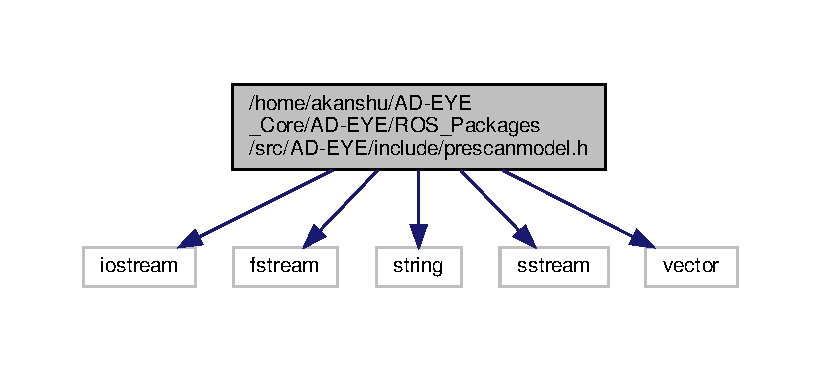
\includegraphics[width=350pt]{prescanmodel_8h__incl}
\end{center}
\end{figure}
This graph shows which files directly or indirectly include this file\+:\nopagebreak
\begin{figure}[H]
\begin{center}
\leavevmode
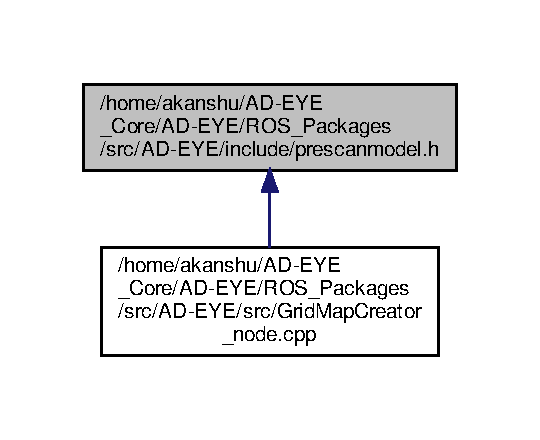
\includegraphics[width=259pt]{prescanmodel_8h__dep__incl}
\end{center}
\end{figure}
\subsection*{Classes}
\begin{DoxyCompactItemize}
\item 
struct \hyperlink{structPrescanObject}{Prescan\+Object}
\begin{DoxyCompactList}\small\item\em This structure handles data from the Prescan Experiment. \end{DoxyCompactList}\item 
struct \hyperlink{structPrescanModel}{Prescan\+Model}
\end{DoxyCompactItemize}
\subsection*{Macros}
\begin{DoxyCompactItemize}
\item 
\#define \hyperlink{prescanmodel_8h_a6096d6d83a92bb558bffe1a87ab6023c}{N\+A\+T\+U\+RE}~0
\item 
\#define \hyperlink{prescanmodel_8h_a7a2ad6ae69001a3457e0c3e311af4bb7}{B\+U\+I\+L\+D\+I\+NG}~1
\item 
\#define \hyperlink{prescanmodel_8h_a6d70b39f611ccb5bc4d2b923af081697}{T\+R\+A\+F\+F\+I\+C\+L\+I\+G\+HT}~2
\item 
\#define \hyperlink{prescanmodel_8h_a521691d53099e69da8c389f92ab58944}{S\+A\+F\+E\+A\+R\+EA}~3
\end{DoxyCompactItemize}


\subsection{Macro Definition Documentation}
\mbox{\Hypertarget{prescanmodel_8h_a7a2ad6ae69001a3457e0c3e311af4bb7}\label{prescanmodel_8h_a7a2ad6ae69001a3457e0c3e311af4bb7}} 
\index{prescanmodel.\+h@{prescanmodel.\+h}!B\+U\+I\+L\+D\+I\+NG@{B\+U\+I\+L\+D\+I\+NG}}
\index{B\+U\+I\+L\+D\+I\+NG@{B\+U\+I\+L\+D\+I\+NG}!prescanmodel.\+h@{prescanmodel.\+h}}
\subsubsection{\texorpdfstring{B\+U\+I\+L\+D\+I\+NG}{BUILDING}}
{\footnotesize\ttfamily \#define B\+U\+I\+L\+D\+I\+NG~1}

\mbox{\Hypertarget{prescanmodel_8h_a6096d6d83a92bb558bffe1a87ab6023c}\label{prescanmodel_8h_a6096d6d83a92bb558bffe1a87ab6023c}} 
\index{prescanmodel.\+h@{prescanmodel.\+h}!N\+A\+T\+U\+RE@{N\+A\+T\+U\+RE}}
\index{N\+A\+T\+U\+RE@{N\+A\+T\+U\+RE}!prescanmodel.\+h@{prescanmodel.\+h}}
\subsubsection{\texorpdfstring{N\+A\+T\+U\+RE}{NATURE}}
{\footnotesize\ttfamily \#define N\+A\+T\+U\+RE~0}

\mbox{\Hypertarget{prescanmodel_8h_a521691d53099e69da8c389f92ab58944}\label{prescanmodel_8h_a521691d53099e69da8c389f92ab58944}} 
\index{prescanmodel.\+h@{prescanmodel.\+h}!S\+A\+F\+E\+A\+R\+EA@{S\+A\+F\+E\+A\+R\+EA}}
\index{S\+A\+F\+E\+A\+R\+EA@{S\+A\+F\+E\+A\+R\+EA}!prescanmodel.\+h@{prescanmodel.\+h}}
\subsubsection{\texorpdfstring{S\+A\+F\+E\+A\+R\+EA}{SAFEAREA}}
{\footnotesize\ttfamily \#define S\+A\+F\+E\+A\+R\+EA~3}

\mbox{\Hypertarget{prescanmodel_8h_a6d70b39f611ccb5bc4d2b923af081697}\label{prescanmodel_8h_a6d70b39f611ccb5bc4d2b923af081697}} 
\index{prescanmodel.\+h@{prescanmodel.\+h}!T\+R\+A\+F\+F\+I\+C\+L\+I\+G\+HT@{T\+R\+A\+F\+F\+I\+C\+L\+I\+G\+HT}}
\index{T\+R\+A\+F\+F\+I\+C\+L\+I\+G\+HT@{T\+R\+A\+F\+F\+I\+C\+L\+I\+G\+HT}!prescanmodel.\+h@{prescanmodel.\+h}}
\subsubsection{\texorpdfstring{T\+R\+A\+F\+F\+I\+C\+L\+I\+G\+HT}{TRAFFICLIGHT}}
{\footnotesize\ttfamily \#define T\+R\+A\+F\+F\+I\+C\+L\+I\+G\+HT~2}


\hypertarget{vectormap_8h}{}\section{/home/akanshu/\+A\+D-\/\+E\+Y\+E\+\_\+\+Core/\+A\+D-\/\+E\+Y\+E/\+R\+O\+S\+\_\+\+Packages/src/\+A\+D-\/\+E\+Y\+E/include/vectormap.h File Reference}
\label{vectormap_8h}\index{/home/akanshu/\+A\+D-\/\+E\+Y\+E\+\_\+\+Core/\+A\+D-\/\+E\+Y\+E/\+R\+O\+S\+\_\+\+Packages/src/\+A\+D-\/\+E\+Y\+E/include/vectormap.\+h@{/home/akanshu/\+A\+D-\/\+E\+Y\+E\+\_\+\+Core/\+A\+D-\/\+E\+Y\+E/\+R\+O\+S\+\_\+\+Packages/src/\+A\+D-\/\+E\+Y\+E/include/vectormap.\+h}}
{\ttfamily \#include $<$iostream$>$}\newline
{\ttfamily \#include $<$fstream$>$}\newline
{\ttfamily \#include $<$string$>$}\newline
{\ttfamily \#include $<$sstream$>$}\newline
{\ttfamily \#include $<$vector$>$}\newline
{\ttfamily \#include $<$cmath$>$}\newline
Include dependency graph for vectormap.\+h\+:\nopagebreak
\begin{figure}[H]
\begin{center}
\leavevmode
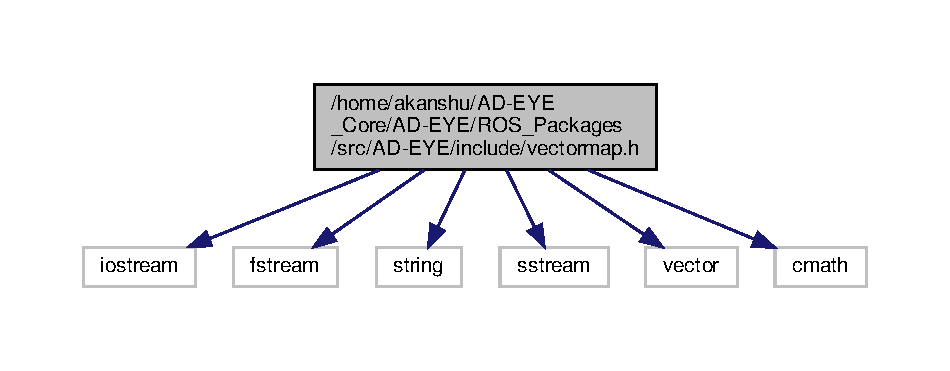
\includegraphics[width=350pt]{vectormap_8h__incl}
\end{center}
\end{figure}
This graph shows which files directly or indirectly include this file\+:\nopagebreak
\begin{figure}[H]
\begin{center}
\leavevmode
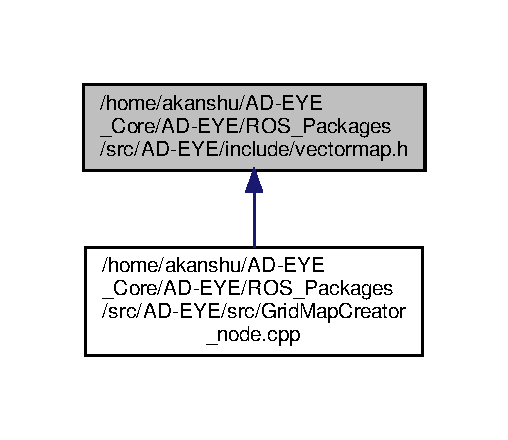
\includegraphics[width=244pt]{vectormap_8h__dep__incl}
\end{center}
\end{figure}
\subsection*{Classes}
\begin{DoxyCompactItemize}
\item 
struct \hyperlink{structVectorMap}{Vector\+Map}
\begin{DoxyCompactList}\small\item\em This structure handles data from the vector map. \end{DoxyCompactList}\end{DoxyCompactItemize}

\hypertarget{camera__info__publisher_8py}{}\section{/home/akanshu/\+A\+D-\/\+E\+Y\+E\+\_\+\+Core/\+A\+D-\/\+E\+Y\+E/\+R\+O\+S\+\_\+\+Packages/src/\+A\+D-\/\+E\+Y\+E/src/camera\+\_\+info\+\_\+publisher.py File Reference}
\label{camera__info__publisher_8py}\index{/home/akanshu/\+A\+D-\/\+E\+Y\+E\+\_\+\+Core/\+A\+D-\/\+E\+Y\+E/\+R\+O\+S\+\_\+\+Packages/src/\+A\+D-\/\+E\+Y\+E/src/camera\+\_\+info\+\_\+publisher.\+py@{/home/akanshu/\+A\+D-\/\+E\+Y\+E\+\_\+\+Core/\+A\+D-\/\+E\+Y\+E/\+R\+O\+S\+\_\+\+Packages/src/\+A\+D-\/\+E\+Y\+E/src/camera\+\_\+info\+\_\+publisher.\+py}}
\subsection*{Namespaces}
\begin{DoxyCompactItemize}
\item 
 \hyperlink{namespacecamera__info__publisher}{camera\+\_\+info\+\_\+publisher}
\end{DoxyCompactItemize}
\subsection*{Variables}
\begin{DoxyCompactItemize}
\item 
\hyperlink{namespacecamera__info__publisher_a2d8ee42f50f0f1a2f44f8287e3d65fde}{camera\+\_\+info\+\_\+publisher.\+msg} = Camera\+Info()
\item 
\hyperlink{namespacecamera__info__publisher_a7f59bda2969259184c03febc1d727bd6}{camera\+\_\+info\+\_\+publisher.\+frame\+\_\+id}
\item 
\hyperlink{namespacecamera__info__publisher_a067a669c555177e826c9b42f9f32fcf3}{camera\+\_\+info\+\_\+publisher.\+height}
\item 
\hyperlink{namespacecamera__info__publisher_a446dc1352be5699a99f9660084e54054}{camera\+\_\+info\+\_\+publisher.\+width}
\item 
\hyperlink{namespacecamera__info__publisher_ab2708da5cf95209018c33acdf374063f}{camera\+\_\+info\+\_\+publisher.\+D}
\item 
\hyperlink{namespacecamera__info__publisher_ae45fa74c6c253f2ebea439d68bdc1fe3}{camera\+\_\+info\+\_\+publisher.\+K}
\item 
\hyperlink{namespacecamera__info__publisher_a9658edfae454ca997cf347704aaa72c3}{camera\+\_\+info\+\_\+publisher.\+R}
\item 
\hyperlink{namespacecamera__info__publisher_a6810e43381f6898ecd0cbedb8a569a7e}{camera\+\_\+info\+\_\+publisher.\+P}
\item 
\hyperlink{namespacecamera__info__publisher_a974733f566916645397703bbee3273d9}{camera\+\_\+info\+\_\+publisher.\+anonymous}
\item 
\hyperlink{namespacecamera__info__publisher_a41969f5fd2d4f608064d7b2d1513450a}{camera\+\_\+info\+\_\+publisher.\+rate} = rospy.\+Rate(10.\+0)
\item 
\hyperlink{namespacecamera__info__publisher_adcc8066d95987066960a2d4861b9a2b9}{camera\+\_\+info\+\_\+publisher.\+pub} = rospy.\+Publisher(sys.\+argv\mbox{[}1\mbox{]}, Camera\+Info, queue\+\_\+size=1)
\end{DoxyCompactItemize}

\hypertarget{cameraObjectListFuse_8cpp}{}\section{/home/akanshu/\+A\+D-\/\+E\+Y\+E\+\_\+\+Core/\+A\+D-\/\+E\+Y\+E/\+R\+O\+S\+\_\+\+Packages/src/\+A\+D-\/\+E\+Y\+E/src/camera\+Object\+List\+Fuse.cpp File Reference}
\label{cameraObjectListFuse_8cpp}\index{/home/akanshu/\+A\+D-\/\+E\+Y\+E\+\_\+\+Core/\+A\+D-\/\+E\+Y\+E/\+R\+O\+S\+\_\+\+Packages/src/\+A\+D-\/\+E\+Y\+E/src/camera\+Object\+List\+Fuse.\+cpp@{/home/akanshu/\+A\+D-\/\+E\+Y\+E\+\_\+\+Core/\+A\+D-\/\+E\+Y\+E/\+R\+O\+S\+\_\+\+Packages/src/\+A\+D-\/\+E\+Y\+E/src/camera\+Object\+List\+Fuse.\+cpp}}
{\ttfamily \#include $<$ros/ros.\+h$>$}\newline
{\ttfamily \#include $<$ros/master.\+h$>$}\newline
{\ttfamily \#include $<$ros/this\+\_\+node.\+h$>$}\newline
{\ttfamily \#include $<$autoware\+\_\+msgs/\+Detected\+Object\+Array.\+h$>$}\newline
Include dependency graph for camera\+Object\+List\+Fuse.\+cpp\+:\nopagebreak
\begin{figure}[H]
\begin{center}
\leavevmode
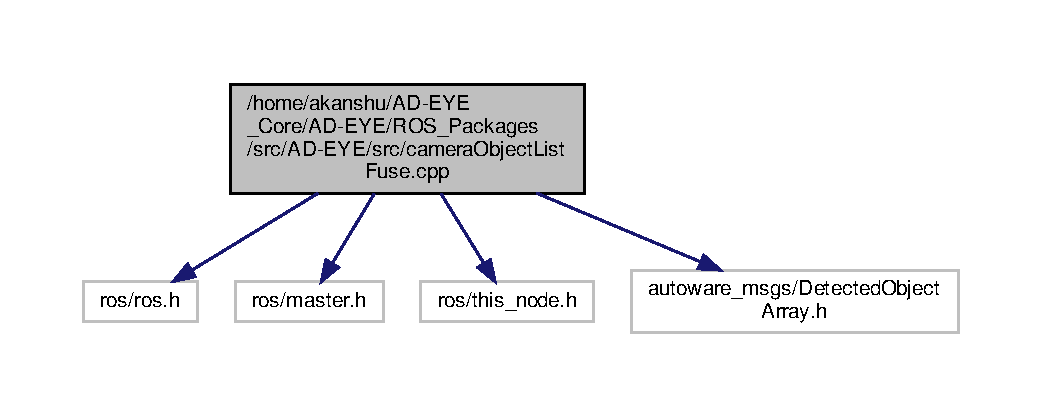
\includegraphics[width=350pt]{cameraObjectListFuse_8cpp__incl}
\end{center}
\end{figure}
\subsection*{Classes}
\begin{DoxyCompactItemize}
\item 
class \hyperlink{classcameraObjectListFuse}{camera\+Object\+List\+Fuse}
\end{DoxyCompactItemize}
\subsection*{Functions}
\begin{DoxyCompactItemize}
\item 
void \hyperlink{cameraObjectListFuse_8cpp_aa89874c10460404be51a149466355178}{usage} (std\+::string bin\+Name)
\item 
int \hyperlink{cameraObjectListFuse_8cpp_a3c04138a5bfe5d72780bb7e82a18e627}{main} (int argc, char $\ast$$\ast$argv)
\end{DoxyCompactItemize}


\subsection{Function Documentation}
\mbox{\Hypertarget{cameraObjectListFuse_8cpp_a3c04138a5bfe5d72780bb7e82a18e627}\label{cameraObjectListFuse_8cpp_a3c04138a5bfe5d72780bb7e82a18e627}} 
\index{camera\+Object\+List\+Fuse.\+cpp@{camera\+Object\+List\+Fuse.\+cpp}!main@{main}}
\index{main@{main}!camera\+Object\+List\+Fuse.\+cpp@{camera\+Object\+List\+Fuse.\+cpp}}
\subsubsection{\texorpdfstring{main()}{main()}}
{\footnotesize\ttfamily int main (\begin{DoxyParamCaption}\item[{int}]{argc,  }\item[{char $\ast$$\ast$}]{argv }\end{DoxyParamCaption})}

\mbox{\Hypertarget{cameraObjectListFuse_8cpp_aa89874c10460404be51a149466355178}\label{cameraObjectListFuse_8cpp_aa89874c10460404be51a149466355178}} 
\index{camera\+Object\+List\+Fuse.\+cpp@{camera\+Object\+List\+Fuse.\+cpp}!usage@{usage}}
\index{usage@{usage}!camera\+Object\+List\+Fuse.\+cpp@{camera\+Object\+List\+Fuse.\+cpp}}
\subsubsection{\texorpdfstring{usage()}{usage()}}
{\footnotesize\ttfamily void usage (\begin{DoxyParamCaption}\item[{std\+::string}]{bin\+Name }\end{DoxyParamCaption})}


\hypertarget{collisionDetector__node_8cpp}{}\section{/home/akanshu/\+A\+D-\/\+E\+Y\+E\+\_\+\+Core/\+A\+D-\/\+E\+Y\+E/\+R\+O\+S\+\_\+\+Packages/src/\+A\+D-\/\+E\+Y\+E/src/collision\+Detector\+\_\+node.cpp File Reference}
\label{collisionDetector__node_8cpp}\index{/home/akanshu/\+A\+D-\/\+E\+Y\+E\+\_\+\+Core/\+A\+D-\/\+E\+Y\+E/\+R\+O\+S\+\_\+\+Packages/src/\+A\+D-\/\+E\+Y\+E/src/collision\+Detector\+\_\+node.\+cpp@{/home/akanshu/\+A\+D-\/\+E\+Y\+E\+\_\+\+Core/\+A\+D-\/\+E\+Y\+E/\+R\+O\+S\+\_\+\+Packages/src/\+A\+D-\/\+E\+Y\+E/src/collision\+Detector\+\_\+node.\+cpp}}
{\ttfamily \#include $<$ros/ros.\+h$>$}\newline
{\ttfamily \#include $<$ros/master.\+h$>$}\newline
{\ttfamily \#include $<$ros/this\+\_\+node.\+h$>$}\newline
{\ttfamily \#include $<$grid\+\_\+map\+\_\+ros/grid\+\_\+map\+\_\+ros.\+hpp$>$}\newline
{\ttfamily \#include $<$grid\+\_\+map\+\_\+msgs/\+Grid\+Map.\+h$>$}\newline
{\ttfamily \#include $<$geometry\+\_\+msgs/\+Pose\+Stamped.\+h$>$}\newline
{\ttfamily \#include $<$geometry\+\_\+msgs/\+Pose.\+h$>$}\newline
{\ttfamily \#include $<$geometry\+\_\+msgs/\+Twist\+Stamped.\+h$>$}\newline
{\ttfamily \#include $<$std\+\_\+msgs/\+Bool.\+h$>$}\newline
{\ttfamily \#include $<$cpp\+\_\+utils/pose\+\_\+datatypes.\+h$>$}\newline
{\ttfamily \#include $<$visualization\+\_\+msgs/\+Marker.\+h$>$}\newline
{\ttfamily \#include $<$std\+\_\+msgs/\+Color\+R\+G\+B\+A.\+h$>$}\newline
Include dependency graph for collision\+Detector\+\_\+node.\+cpp\+:\nopagebreak
\begin{figure}[H]
\begin{center}
\leavevmode
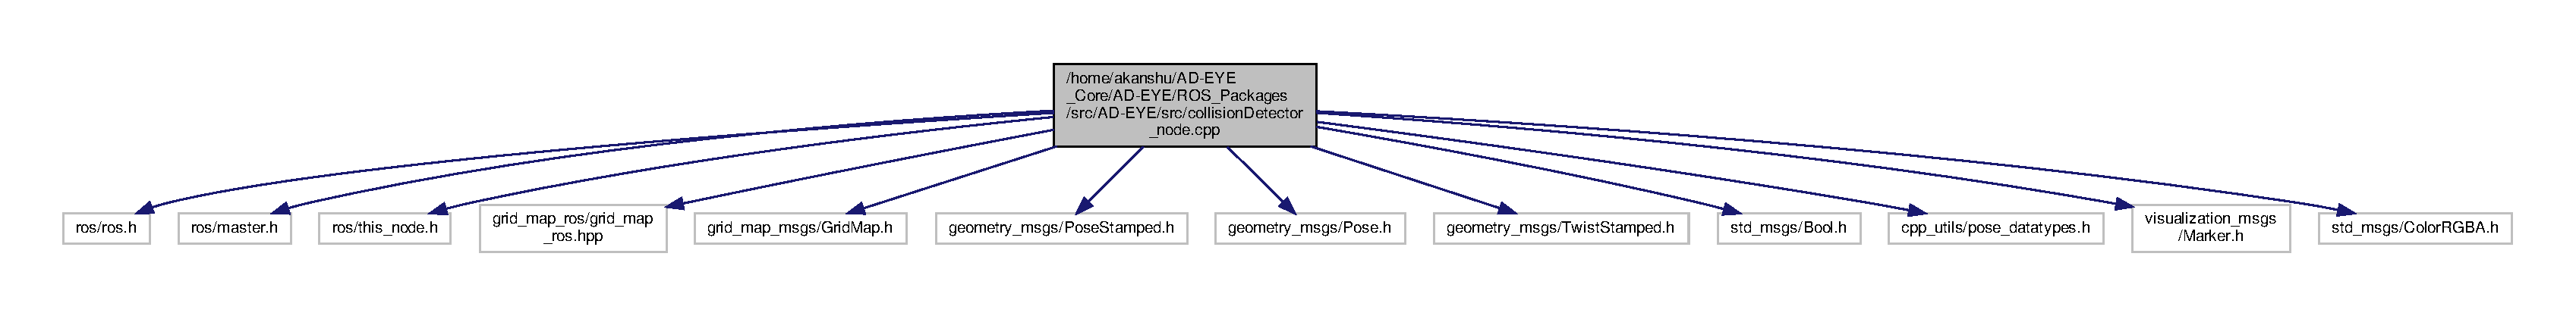
\includegraphics[width=350pt]{collisionDetector__node_8cpp__incl}
\end{center}
\end{figure}
\subsection*{Classes}
\begin{DoxyCompactItemize}
\item 
class \hyperlink{classCollisionDetector}{Collision\+Detector}
\begin{DoxyCompactList}\small\item\em A node that detect collision with other objects using the S\+S\+M\+P\+\_\+grid\+Map. \end{DoxyCompactList}\end{DoxyCompactItemize}
\subsection*{Functions}
\begin{DoxyCompactItemize}
\item 
int \hyperlink{collisionDetector__node_8cpp_a3c04138a5bfe5d72780bb7e82a18e627}{main} (int argc, char $\ast$$\ast$argv)
\end{DoxyCompactItemize}


\subsection{Function Documentation}
\mbox{\Hypertarget{collisionDetector__node_8cpp_a3c04138a5bfe5d72780bb7e82a18e627}\label{collisionDetector__node_8cpp_a3c04138a5bfe5d72780bb7e82a18e627}} 
\index{collision\+Detector\+\_\+node.\+cpp@{collision\+Detector\+\_\+node.\+cpp}!main@{main}}
\index{main@{main}!collision\+Detector\+\_\+node.\+cpp@{collision\+Detector\+\_\+node.\+cpp}}
\subsubsection{\texorpdfstring{main()}{main()}}
{\footnotesize\ttfamily int main (\begin{DoxyParamCaption}\item[{int}]{argc,  }\item[{char $\ast$$\ast$}]{argv }\end{DoxyParamCaption})}


\hypertarget{controlSwitch__node_8cpp}{}\section{/home/akanshu/\+A\+D-\/\+E\+Y\+E\+\_\+\+Core/\+A\+D-\/\+E\+Y\+E/\+R\+O\+S\+\_\+\+Packages/src/\+A\+D-\/\+E\+Y\+E/src/control\+Switch\+\_\+node.cpp File Reference}
\label{controlSwitch__node_8cpp}\index{/home/akanshu/\+A\+D-\/\+E\+Y\+E\+\_\+\+Core/\+A\+D-\/\+E\+Y\+E/\+R\+O\+S\+\_\+\+Packages/src/\+A\+D-\/\+E\+Y\+E/src/control\+Switch\+\_\+node.\+cpp@{/home/akanshu/\+A\+D-\/\+E\+Y\+E\+\_\+\+Core/\+A\+D-\/\+E\+Y\+E/\+R\+O\+S\+\_\+\+Packages/src/\+A\+D-\/\+E\+Y\+E/src/control\+Switch\+\_\+node.\+cpp}}
{\ttfamily \#include $<$ros/ros.\+h$>$}\newline
{\ttfamily \#include $<$vector$>$}\newline
{\ttfamily \#include $<$string$>$}\newline
{\ttfamily \#include $<$cmath$>$}\newline
{\ttfamily \#include $<$stdlib.\+h$>$}\newline
{\ttfamily \#include $<$limits$>$}\newline
{\ttfamily \#include $<$geometry\+\_\+msgs/\+Polygon\+Stamped.\+h$>$}\newline
{\ttfamily \#include $<$tf/transform\+\_\+listener.\+h$>$}\newline
{\ttfamily \#include $<$tf/transform\+\_\+broadcaster.\+h$>$}\newline
{\ttfamily \#include $<$rcv\+\_\+common\+\_\+msgs/trajectory\+\_\+reference.\+h$>$}\newline
{\ttfamily \#include $<$rcv\+\_\+common\+\_\+msgs/current\+\_\+traj\+\_\+info.\+h$>$}\newline
{\ttfamily \#include $<$rcv\+\_\+common\+\_\+msgs/\+S\+S\+M\+P\+\_\+control.\+h$>$}\newline
{\ttfamily \#include $<$nav\+\_\+msgs/\+Odometry.\+h$>$}\newline
{\ttfamily \#include $<$cpp\+\_\+utils/pose\+\_\+datatypes.\+h$>$}\newline
{\ttfamily \#include $<$std\+\_\+msgs/\+Int32.\+h$>$}\newline
Include dependency graph for control\+Switch\+\_\+node.\+cpp\+:\nopagebreak
\begin{figure}[H]
\begin{center}
\leavevmode
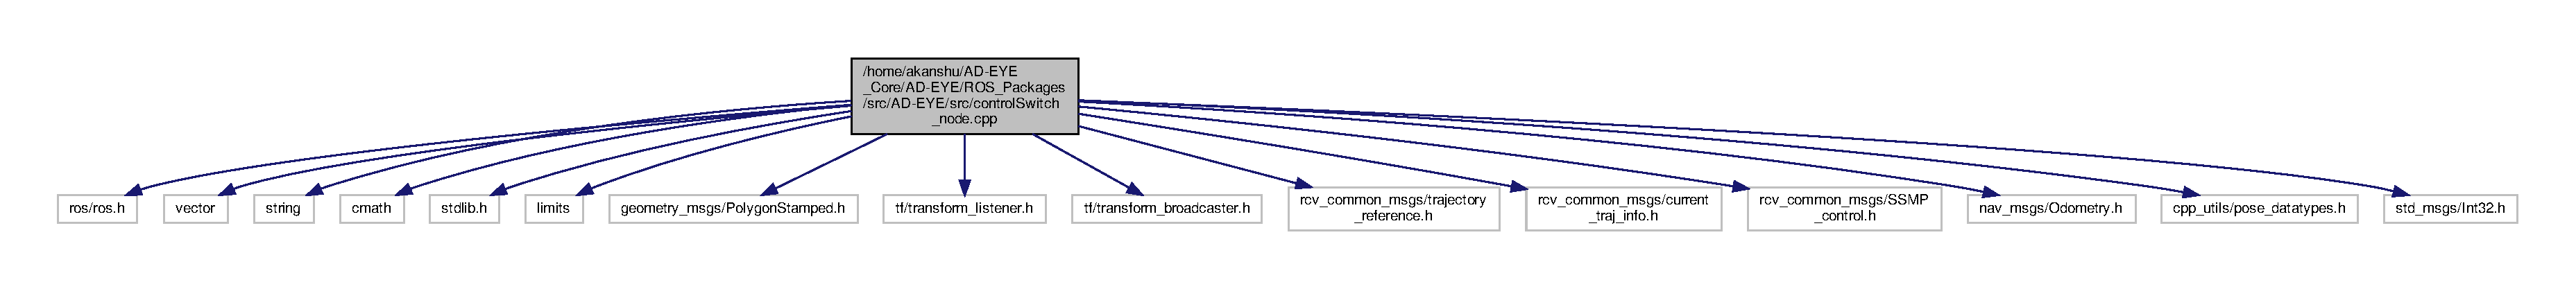
\includegraphics[width=350pt]{controlSwitch__node_8cpp__incl}
\end{center}
\end{figure}
\subsection*{Classes}
\begin{DoxyCompactItemize}
\item 
class \hyperlink{classcontrolSwitch}{control\+Switch}
\begin{DoxyCompactList}\small\item\em This class is the Switch that selects which channel control the car. \end{DoxyCompactList}\end{DoxyCompactItemize}
\subsection*{Macros}
\begin{DoxyCompactItemize}
\item 
\#define \hyperlink{controlSwitch__node_8cpp_a5d1e380ee82e7ec17b946c3f57affb95}{A\+U\+T\+O\+W\+A\+RE}~0
\item 
\#define \hyperlink{controlSwitch__node_8cpp_ae9ee2d0cbf0e6cfa2822c4eb3f75e04b}{S\+S\+MP}~1
\end{DoxyCompactItemize}
\subsection*{Functions}
\begin{DoxyCompactItemize}
\item 
int \hyperlink{controlSwitch__node_8cpp_a3c04138a5bfe5d72780bb7e82a18e627}{main} (int argc, char $\ast$$\ast$argv)
\end{DoxyCompactItemize}


\subsection{Macro Definition Documentation}
\mbox{\Hypertarget{controlSwitch__node_8cpp_a5d1e380ee82e7ec17b946c3f57affb95}\label{controlSwitch__node_8cpp_a5d1e380ee82e7ec17b946c3f57affb95}} 
\index{control\+Switch\+\_\+node.\+cpp@{control\+Switch\+\_\+node.\+cpp}!A\+U\+T\+O\+W\+A\+RE@{A\+U\+T\+O\+W\+A\+RE}}
\index{A\+U\+T\+O\+W\+A\+RE@{A\+U\+T\+O\+W\+A\+RE}!control\+Switch\+\_\+node.\+cpp@{control\+Switch\+\_\+node.\+cpp}}
\subsubsection{\texorpdfstring{A\+U\+T\+O\+W\+A\+RE}{AUTOWARE}}
{\footnotesize\ttfamily \#define A\+U\+T\+O\+W\+A\+RE~0}

\mbox{\Hypertarget{controlSwitch__node_8cpp_ae9ee2d0cbf0e6cfa2822c4eb3f75e04b}\label{controlSwitch__node_8cpp_ae9ee2d0cbf0e6cfa2822c4eb3f75e04b}} 
\index{control\+Switch\+\_\+node.\+cpp@{control\+Switch\+\_\+node.\+cpp}!S\+S\+MP@{S\+S\+MP}}
\index{S\+S\+MP@{S\+S\+MP}!control\+Switch\+\_\+node.\+cpp@{control\+Switch\+\_\+node.\+cpp}}
\subsubsection{\texorpdfstring{S\+S\+MP}{SSMP}}
{\footnotesize\ttfamily \#define S\+S\+MP~1}



\subsection{Function Documentation}
\mbox{\Hypertarget{controlSwitch__node_8cpp_a3c04138a5bfe5d72780bb7e82a18e627}\label{controlSwitch__node_8cpp_a3c04138a5bfe5d72780bb7e82a18e627}} 
\index{control\+Switch\+\_\+node.\+cpp@{control\+Switch\+\_\+node.\+cpp}!main@{main}}
\index{main@{main}!control\+Switch\+\_\+node.\+cpp@{control\+Switch\+\_\+node.\+cpp}}
\subsubsection{\texorpdfstring{main()}{main()}}
{\footnotesize\ttfamily int main (\begin{DoxyParamCaption}\item[{int}]{argc,  }\item[{char $\ast$$\ast$}]{argv }\end{DoxyParamCaption})}


\hypertarget{FeatureControl_8py}{}\section{/home/akanshu/\+A\+D-\/\+E\+Y\+E\+\_\+\+Core/\+A\+D-\/\+E\+Y\+E/\+R\+O\+S\+\_\+\+Packages/src/\+A\+D-\/\+E\+Y\+E/src/\+Feature\+Control.py File Reference}
\label{FeatureControl_8py}\index{/home/akanshu/\+A\+D-\/\+E\+Y\+E\+\_\+\+Core/\+A\+D-\/\+E\+Y\+E/\+R\+O\+S\+\_\+\+Packages/src/\+A\+D-\/\+E\+Y\+E/src/\+Feature\+Control.\+py@{/home/akanshu/\+A\+D-\/\+E\+Y\+E\+\_\+\+Core/\+A\+D-\/\+E\+Y\+E/\+R\+O\+S\+\_\+\+Packages/src/\+A\+D-\/\+E\+Y\+E/src/\+Feature\+Control.\+py}}
\subsection*{Classes}
\begin{DoxyCompactItemize}
\item 
class \hyperlink{classFeatureControl_1_1FeatureControl}{Feature\+Control.\+Feature\+Control}
\end{DoxyCompactItemize}
\subsection*{Namespaces}
\begin{DoxyCompactItemize}
\item 
 \hyperlink{namespaceFeatureControl}{Feature\+Control}
\end{DoxyCompactItemize}
\subsection*{Variables}
\begin{DoxyCompactItemize}
\item 
float \hyperlink{namespaceFeatureControl_aeebd4e13e6a3a0dde7d720af530ae36d}{Feature\+Control.\+D\+E\+F\+A\+U\+L\+T\+\_\+\+W\+A\+I\+T\+\_\+\+T\+I\+ME} = 0.\+1
\end{DoxyCompactItemize}

\hypertarget{flattening__node_8cpp}{}\section{/home/akanshu/\+A\+D-\/\+E\+Y\+E\+\_\+\+Core/\+A\+D-\/\+E\+Y\+E/\+R\+O\+S\+\_\+\+Packages/src/\+A\+D-\/\+E\+Y\+E/src/flattening\+\_\+node.cpp File Reference}
\label{flattening__node_8cpp}\index{/home/akanshu/\+A\+D-\/\+E\+Y\+E\+\_\+\+Core/\+A\+D-\/\+E\+Y\+E/\+R\+O\+S\+\_\+\+Packages/src/\+A\+D-\/\+E\+Y\+E/src/flattening\+\_\+node.\+cpp@{/home/akanshu/\+A\+D-\/\+E\+Y\+E\+\_\+\+Core/\+A\+D-\/\+E\+Y\+E/\+R\+O\+S\+\_\+\+Packages/src/\+A\+D-\/\+E\+Y\+E/src/flattening\+\_\+node.\+cpp}}
{\ttfamily \#include $<$ros/ros.\+h$>$}\newline
{\ttfamily \#include $<$grid\+\_\+map\+\_\+ros/grid\+\_\+map\+\_\+ros.\+hpp$>$}\newline
{\ttfamily \#include $<$grid\+\_\+map\+\_\+msgs/\+Grid\+Map.\+h$>$}\newline
{\ttfamily \#include $<$grid\+\_\+map\+\_\+ros/\+Grid\+Map\+Ros\+Converter.\+hpp$>$}\newline
{\ttfamily \#include $<$vector$>$}\newline
{\ttfamily \#include $<$string$>$}\newline
{\ttfamily \#include $<$cmath$>$}\newline
{\ttfamily \#include $<$stdlib.\+h$>$}\newline
{\ttfamily \#include $<$limits$>$}\newline
{\ttfamily \#include $<$nav\+\_\+msgs/\+Occupancy\+Grid.\+h$>$}\newline
{\ttfamily \#include $<$nav\+\_\+msgs/\+Odometry.\+h$>$}\newline
{\ttfamily \#include $<$tf/transform\+\_\+broadcaster.\+h$>$}\newline
{\ttfamily \#include $<$cpp\+\_\+utils/pose\+\_\+datatypes.\+h$>$}\newline
Include dependency graph for flattening\+\_\+node.\+cpp\+:\nopagebreak
\begin{figure}[H]
\begin{center}
\leavevmode
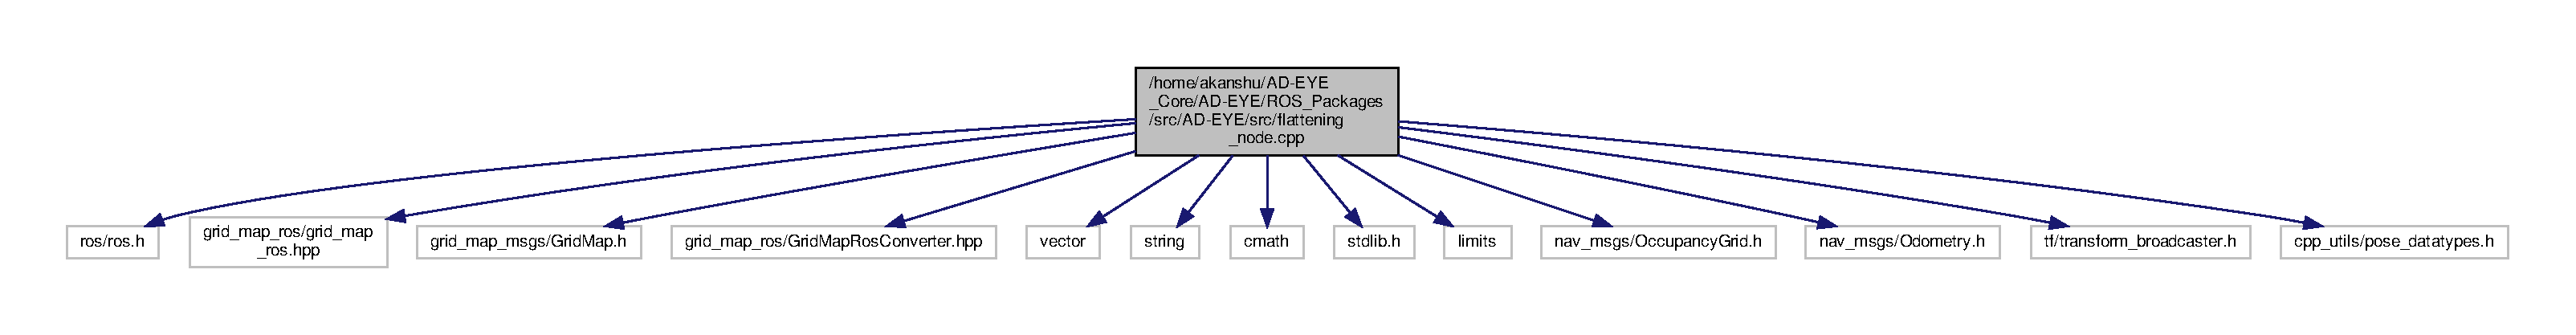
\includegraphics[width=350pt]{flattening__node_8cpp__incl}
\end{center}
\end{figure}
\subsection*{Classes}
\begin{DoxyCompactItemize}
\item 
class \hyperlink{classOccMapCreator}{Occ\+Map\+Creator}
\begin{DoxyCompactList}\small\item\em This class is used to extract data from the Grid\+Map given by the \hyperlink{classGridMapCreator}{Grid\+Map\+Creator}. \end{DoxyCompactList}\end{DoxyCompactItemize}
\subsection*{Macros}
\begin{DoxyCompactItemize}
\item 
\#define \hyperlink{flattening__node_8cpp_a87b537f5fa5c109d3c05c13d6b18f382}{W\+H\+I\+TE}~1
\item 
\#define \hyperlink{flattening__node_8cpp_acfbc006ea433ad708fdee3e82996e721}{G\+R\+E\+EN}~30
\item 
\#define \hyperlink{flattening__node_8cpp_abf681265909adf3d3e8116c93c0ba179}{Y\+E\+L\+L\+OW}~50
\item 
\#define \hyperlink{flattening__node_8cpp_a8d23feea868a983c8c2b661e1e16972f}{R\+ED}~99
\end{DoxyCompactItemize}
\subsection*{Functions}
\begin{DoxyCompactItemize}
\item 
void \hyperlink{flattening__node_8cpp_aa89874c10460404be51a149466355178}{usage} (std\+::string bin\+Name)
\item 
int \hyperlink{flattening__node_8cpp_a3c04138a5bfe5d72780bb7e82a18e627}{main} (int argc, char $\ast$$\ast$argv)
\end{DoxyCompactItemize}


\subsection{Macro Definition Documentation}
\mbox{\Hypertarget{flattening__node_8cpp_acfbc006ea433ad708fdee3e82996e721}\label{flattening__node_8cpp_acfbc006ea433ad708fdee3e82996e721}} 
\index{flattening\+\_\+node.\+cpp@{flattening\+\_\+node.\+cpp}!G\+R\+E\+EN@{G\+R\+E\+EN}}
\index{G\+R\+E\+EN@{G\+R\+E\+EN}!flattening\+\_\+node.\+cpp@{flattening\+\_\+node.\+cpp}}
\subsubsection{\texorpdfstring{G\+R\+E\+EN}{GREEN}}
{\footnotesize\ttfamily \#define G\+R\+E\+EN~30}

\mbox{\Hypertarget{flattening__node_8cpp_a8d23feea868a983c8c2b661e1e16972f}\label{flattening__node_8cpp_a8d23feea868a983c8c2b661e1e16972f}} 
\index{flattening\+\_\+node.\+cpp@{flattening\+\_\+node.\+cpp}!R\+ED@{R\+ED}}
\index{R\+ED@{R\+ED}!flattening\+\_\+node.\+cpp@{flattening\+\_\+node.\+cpp}}
\subsubsection{\texorpdfstring{R\+ED}{RED}}
{\footnotesize\ttfamily \#define R\+ED~99}

\mbox{\Hypertarget{flattening__node_8cpp_a87b537f5fa5c109d3c05c13d6b18f382}\label{flattening__node_8cpp_a87b537f5fa5c109d3c05c13d6b18f382}} 
\index{flattening\+\_\+node.\+cpp@{flattening\+\_\+node.\+cpp}!W\+H\+I\+TE@{W\+H\+I\+TE}}
\index{W\+H\+I\+TE@{W\+H\+I\+TE}!flattening\+\_\+node.\+cpp@{flattening\+\_\+node.\+cpp}}
\subsubsection{\texorpdfstring{W\+H\+I\+TE}{WHITE}}
{\footnotesize\ttfamily \#define W\+H\+I\+TE~1}

\mbox{\Hypertarget{flattening__node_8cpp_abf681265909adf3d3e8116c93c0ba179}\label{flattening__node_8cpp_abf681265909adf3d3e8116c93c0ba179}} 
\index{flattening\+\_\+node.\+cpp@{flattening\+\_\+node.\+cpp}!Y\+E\+L\+L\+OW@{Y\+E\+L\+L\+OW}}
\index{Y\+E\+L\+L\+OW@{Y\+E\+L\+L\+OW}!flattening\+\_\+node.\+cpp@{flattening\+\_\+node.\+cpp}}
\subsubsection{\texorpdfstring{Y\+E\+L\+L\+OW}{YELLOW}}
{\footnotesize\ttfamily \#define Y\+E\+L\+L\+OW~50}



\subsection{Function Documentation}
\mbox{\Hypertarget{flattening__node_8cpp_a3c04138a5bfe5d72780bb7e82a18e627}\label{flattening__node_8cpp_a3c04138a5bfe5d72780bb7e82a18e627}} 
\index{flattening\+\_\+node.\+cpp@{flattening\+\_\+node.\+cpp}!main@{main}}
\index{main@{main}!flattening\+\_\+node.\+cpp@{flattening\+\_\+node.\+cpp}}
\subsubsection{\texorpdfstring{main()}{main()}}
{\footnotesize\ttfamily int main (\begin{DoxyParamCaption}\item[{int}]{argc,  }\item[{char $\ast$$\ast$}]{argv }\end{DoxyParamCaption})}

\mbox{\Hypertarget{flattening__node_8cpp_aa89874c10460404be51a149466355178}\label{flattening__node_8cpp_aa89874c10460404be51a149466355178}} 
\index{flattening\+\_\+node.\+cpp@{flattening\+\_\+node.\+cpp}!usage@{usage}}
\index{usage@{usage}!flattening\+\_\+node.\+cpp@{flattening\+\_\+node.\+cpp}}
\subsubsection{\texorpdfstring{usage()}{usage()}}
{\footnotesize\ttfamily void usage (\begin{DoxyParamCaption}\item[{std\+::string}]{bin\+Name }\end{DoxyParamCaption})}


\hypertarget{gnss__broadcaster_8py}{}\section{/home/akanshu/\+A\+D-\/\+E\+Y\+E\+\_\+\+Core/\+A\+D-\/\+E\+Y\+E/\+R\+O\+S\+\_\+\+Packages/src/\+A\+D-\/\+E\+Y\+E/src/gnss\+\_\+broadcaster.py File Reference}
\label{gnss__broadcaster_8py}\index{/home/akanshu/\+A\+D-\/\+E\+Y\+E\+\_\+\+Core/\+A\+D-\/\+E\+Y\+E/\+R\+O\+S\+\_\+\+Packages/src/\+A\+D-\/\+E\+Y\+E/src/gnss\+\_\+broadcaster.\+py@{/home/akanshu/\+A\+D-\/\+E\+Y\+E\+\_\+\+Core/\+A\+D-\/\+E\+Y\+E/\+R\+O\+S\+\_\+\+Packages/src/\+A\+D-\/\+E\+Y\+E/src/gnss\+\_\+broadcaster.\+py}}
\subsection*{Namespaces}
\begin{DoxyCompactItemize}
\item 
 \hyperlink{namespacegnss__broadcaster}{gnss\+\_\+broadcaster}
\end{DoxyCompactItemize}
\subsection*{Functions}
\begin{DoxyCompactItemize}
\item 
def \hyperlink{namespacegnss__broadcaster_a0476bd17f38f4829ece1fde1e939ace2}{gnss\+\_\+broadcaster.\+mycallback} (data)
\end{DoxyCompactItemize}

\hypertarget{GridMapCreator__node_8cpp}{}\section{/home/akanshu/\+A\+D-\/\+E\+Y\+E\+\_\+\+Core/\+A\+D-\/\+E\+Y\+E/\+R\+O\+S\+\_\+\+Packages/src/\+A\+D-\/\+E\+Y\+E/src/\+Grid\+Map\+Creator\+\_\+node.cpp File Reference}
\label{GridMapCreator__node_8cpp}\index{/home/akanshu/\+A\+D-\/\+E\+Y\+E\+\_\+\+Core/\+A\+D-\/\+E\+Y\+E/\+R\+O\+S\+\_\+\+Packages/src/\+A\+D-\/\+E\+Y\+E/src/\+Grid\+Map\+Creator\+\_\+node.\+cpp@{/home/akanshu/\+A\+D-\/\+E\+Y\+E\+\_\+\+Core/\+A\+D-\/\+E\+Y\+E/\+R\+O\+S\+\_\+\+Packages/src/\+A\+D-\/\+E\+Y\+E/src/\+Grid\+Map\+Creator\+\_\+node.\+cpp}}
{\ttfamily \#include $<$ros/ros.\+h$>$}\newline
{\ttfamily \#include $<$grid\+\_\+map\+\_\+ros/grid\+\_\+map\+\_\+ros.\+hpp$>$}\newline
{\ttfamily \#include $<$grid\+\_\+map\+\_\+msgs/\+Grid\+Map.\+h$>$}\newline
{\ttfamily \#include $<$vector$>$}\newline
{\ttfamily \#include $<$string$>$}\newline
{\ttfamily \#include $<$cmath$>$}\newline
{\ttfamily \#include $<$stdlib.\+h$>$}\newline
{\ttfamily \#include $<$limits$>$}\newline
{\ttfamily \#include $<$nav\+\_\+msgs/\+Occupancy\+Grid.\+h$>$}\newline
{\ttfamily \#include $<$nav\+\_\+msgs/\+Odometry.\+h$>$}\newline
{\ttfamily \#include $<$vectormap.\+h$>$}\newline
{\ttfamily \#include $<$prescanmodel.\+h$>$}\newline
{\ttfamily \#include $<$tf/transform\+\_\+listener.\+h$>$}\newline
{\ttfamily \#include $<$tf/transform\+\_\+broadcaster.\+h$>$}\newline
{\ttfamily \#include $<$rcv\+\_\+common\+\_\+msgs/\+S\+S\+M\+P\+\_\+control.\+h$>$}\newline
{\ttfamily \#include $<$cpp\+\_\+utils/pose\+\_\+datatypes.\+h$>$}\newline
{\ttfamily \#include $<$geometry\+\_\+msgs/\+Pose\+Array.\+h$>$}\newline
{\ttfamily \#include $<$dirent.\+h$>$}\newline
Include dependency graph for Grid\+Map\+Creator\+\_\+node.\+cpp\+:\nopagebreak
\begin{figure}[H]
\begin{center}
\leavevmode
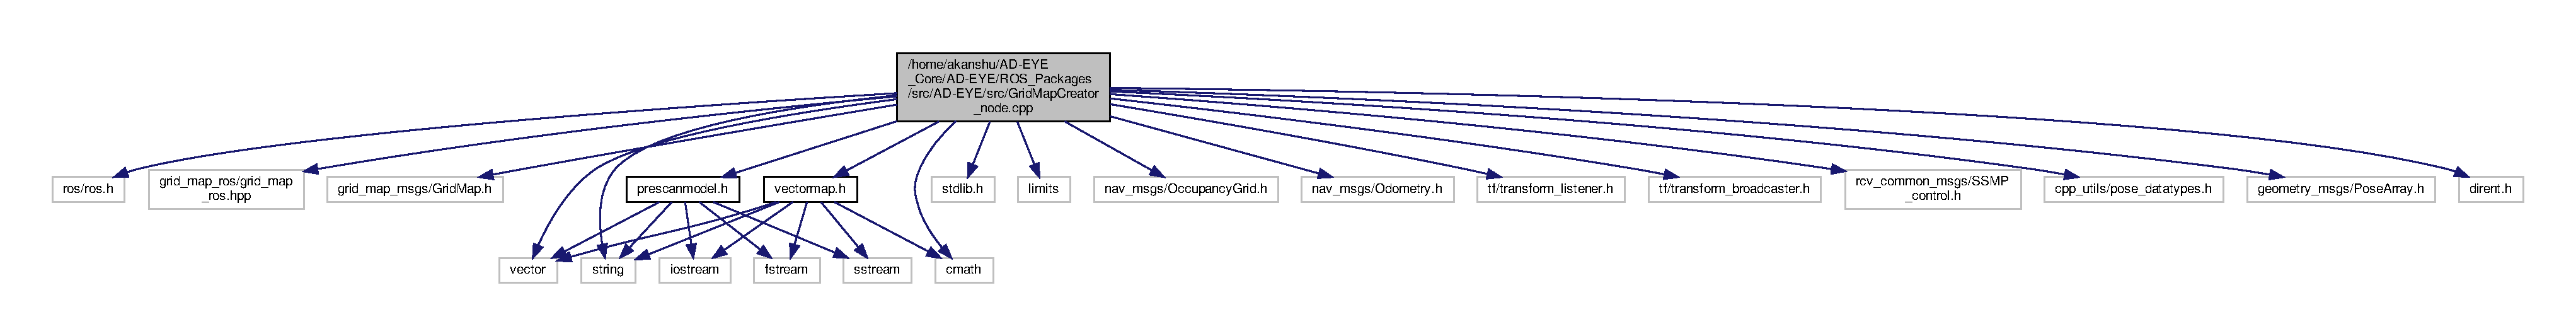
\includegraphics[width=350pt]{GridMapCreator__node_8cpp__incl}
\end{center}
\end{figure}
\subsection*{Classes}
\begin{DoxyCompactItemize}
\item 
class \hyperlink{classGridMapCreator}{Grid\+Map\+Creator}
\begin{DoxyCompactList}\small\item\em The \hyperlink{classGridMapCreator}{Grid\+Map\+Creator} maintains a grid map used to know where safe places are. \end{DoxyCompactList}\end{DoxyCompactItemize}
\subsection*{Macros}
\begin{DoxyCompactItemize}
\item 
\#define \hyperlink{GridMapCreator__node_8cpp_ae3ec3219e4eee3b0992bfd59c2e2bc42}{H\+A\+L\+F\+\_\+\+PI}~1.\+5708
\end{DoxyCompactItemize}
\subsection*{Functions}
\begin{DoxyCompactItemize}
\item 
void \hyperlink{GridMapCreator__node_8cpp_aa89874c10460404be51a149466355178}{usage} (std\+::string bin\+Name)
\begin{DoxyCompactList}\small\item\em Print a help message on how to use the node. \end{DoxyCompactList}\item 
int \hyperlink{GridMapCreator__node_8cpp_a3c04138a5bfe5d72780bb7e82a18e627}{main} (int argc, char $\ast$$\ast$argv)
\end{DoxyCompactItemize}


\subsection{Macro Definition Documentation}
\mbox{\Hypertarget{GridMapCreator__node_8cpp_ae3ec3219e4eee3b0992bfd59c2e2bc42}\label{GridMapCreator__node_8cpp_ae3ec3219e4eee3b0992bfd59c2e2bc42}} 
\index{Grid\+Map\+Creator\+\_\+node.\+cpp@{Grid\+Map\+Creator\+\_\+node.\+cpp}!H\+A\+L\+F\+\_\+\+PI@{H\+A\+L\+F\+\_\+\+PI}}
\index{H\+A\+L\+F\+\_\+\+PI@{H\+A\+L\+F\+\_\+\+PI}!Grid\+Map\+Creator\+\_\+node.\+cpp@{Grid\+Map\+Creator\+\_\+node.\+cpp}}
\subsubsection{\texorpdfstring{H\+A\+L\+F\+\_\+\+PI}{HALF\_PI}}
{\footnotesize\ttfamily \#define H\+A\+L\+F\+\_\+\+PI~1.\+5708}



\subsection{Function Documentation}
\mbox{\Hypertarget{GridMapCreator__node_8cpp_a3c04138a5bfe5d72780bb7e82a18e627}\label{GridMapCreator__node_8cpp_a3c04138a5bfe5d72780bb7e82a18e627}} 
\index{Grid\+Map\+Creator\+\_\+node.\+cpp@{Grid\+Map\+Creator\+\_\+node.\+cpp}!main@{main}}
\index{main@{main}!Grid\+Map\+Creator\+\_\+node.\+cpp@{Grid\+Map\+Creator\+\_\+node.\+cpp}}
\subsubsection{\texorpdfstring{main()}{main()}}
{\footnotesize\ttfamily int main (\begin{DoxyParamCaption}\item[{int}]{argc,  }\item[{char $\ast$$\ast$}]{argv }\end{DoxyParamCaption})}

\mbox{\Hypertarget{GridMapCreator__node_8cpp_aa89874c10460404be51a149466355178}\label{GridMapCreator__node_8cpp_aa89874c10460404be51a149466355178}} 
\index{Grid\+Map\+Creator\+\_\+node.\+cpp@{Grid\+Map\+Creator\+\_\+node.\+cpp}!usage@{usage}}
\index{usage@{usage}!Grid\+Map\+Creator\+\_\+node.\+cpp@{Grid\+Map\+Creator\+\_\+node.\+cpp}}
\subsubsection{\texorpdfstring{usage()}{usage()}}
{\footnotesize\ttfamily void usage (\begin{DoxyParamCaption}\item[{std\+::string}]{bin\+Name }\end{DoxyParamCaption})}



Print a help message on how to use the node. 

Specify arguments needed 
\hypertarget{lidarRadarFuse_8cpp}{}\section{/home/akanshu/\+A\+D-\/\+E\+Y\+E\+\_\+\+Core/\+A\+D-\/\+E\+Y\+E/\+R\+O\+S\+\_\+\+Packages/src/\+A\+D-\/\+E\+Y\+E/src/lidar\+Radar\+Fuse.cpp File Reference}
\label{lidarRadarFuse_8cpp}\index{/home/akanshu/\+A\+D-\/\+E\+Y\+E\+\_\+\+Core/\+A\+D-\/\+E\+Y\+E/\+R\+O\+S\+\_\+\+Packages/src/\+A\+D-\/\+E\+Y\+E/src/lidar\+Radar\+Fuse.\+cpp@{/home/akanshu/\+A\+D-\/\+E\+Y\+E\+\_\+\+Core/\+A\+D-\/\+E\+Y\+E/\+R\+O\+S\+\_\+\+Packages/src/\+A\+D-\/\+E\+Y\+E/src/lidar\+Radar\+Fuse.\+cpp}}
{\ttfamily \#include $<$ros/ros.\+h$>$}\newline
{\ttfamily \#include $<$ros/master.\+h$>$}\newline
{\ttfamily \#include $<$ros/this\+\_\+node.\+h$>$}\newline
{\ttfamily \#include $<$autoware\+\_\+msgs/\+Detected\+Object\+Array.\+h$>$}\newline
{\ttfamily \#include $<$geometry\+\_\+msgs/\+Point.\+h$>$}\newline
Include dependency graph for lidar\+Radar\+Fuse.\+cpp\+:\nopagebreak
\begin{figure}[H]
\begin{center}
\leavevmode
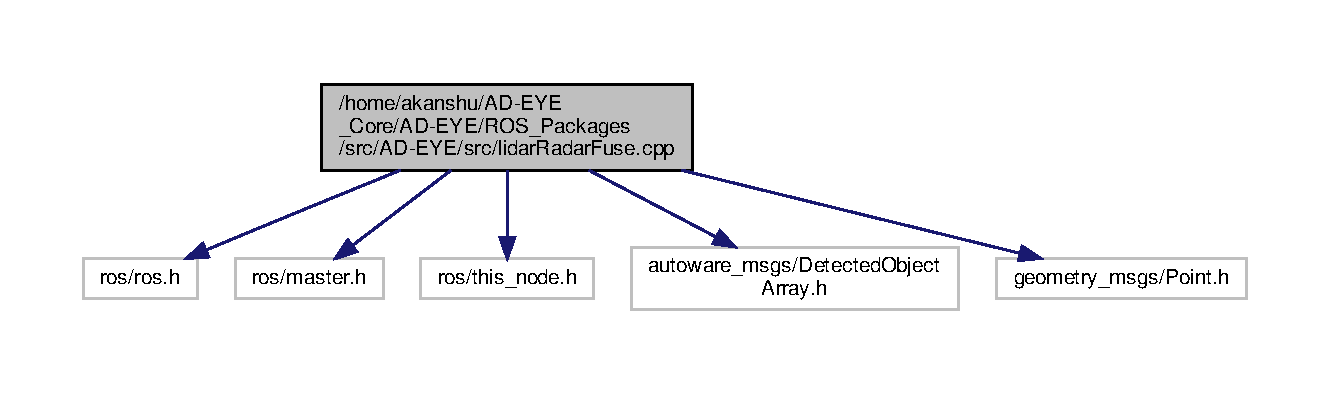
\includegraphics[width=350pt]{lidarRadarFuse_8cpp__incl}
\end{center}
\end{figure}
\subsection*{Classes}
\begin{DoxyCompactItemize}
\item 
class \hyperlink{classlidarRadarFuse}{lidar\+Radar\+Fuse}
\end{DoxyCompactItemize}
\subsection*{Macros}
\begin{DoxyCompactItemize}
\item 
\#define \hyperlink{lidarRadarFuse_8cpp_a93a1658d86010dfb4f73384a83f1a942}{R\+A\+D\+A\+R\+\_\+\+L\+I\+D\+A\+R\+\_\+\+M\+A\+X\+\_\+\+D\+I\+S\+T\+A\+N\+CE}~1
\end{DoxyCompactItemize}
\subsection*{Functions}
\begin{DoxyCompactItemize}
\item 
void \hyperlink{lidarRadarFuse_8cpp_aa89874c10460404be51a149466355178}{usage} (std\+::string bin\+Name)
\item 
int \hyperlink{lidarRadarFuse_8cpp_a3c04138a5bfe5d72780bb7e82a18e627}{main} (int argc, char $\ast$$\ast$argv)
\end{DoxyCompactItemize}


\subsection{Macro Definition Documentation}
\mbox{\Hypertarget{lidarRadarFuse_8cpp_a93a1658d86010dfb4f73384a83f1a942}\label{lidarRadarFuse_8cpp_a93a1658d86010dfb4f73384a83f1a942}} 
\index{lidar\+Radar\+Fuse.\+cpp@{lidar\+Radar\+Fuse.\+cpp}!R\+A\+D\+A\+R\+\_\+\+L\+I\+D\+A\+R\+\_\+\+M\+A\+X\+\_\+\+D\+I\+S\+T\+A\+N\+CE@{R\+A\+D\+A\+R\+\_\+\+L\+I\+D\+A\+R\+\_\+\+M\+A\+X\+\_\+\+D\+I\+S\+T\+A\+N\+CE}}
\index{R\+A\+D\+A\+R\+\_\+\+L\+I\+D\+A\+R\+\_\+\+M\+A\+X\+\_\+\+D\+I\+S\+T\+A\+N\+CE@{R\+A\+D\+A\+R\+\_\+\+L\+I\+D\+A\+R\+\_\+\+M\+A\+X\+\_\+\+D\+I\+S\+T\+A\+N\+CE}!lidar\+Radar\+Fuse.\+cpp@{lidar\+Radar\+Fuse.\+cpp}}
\subsubsection{\texorpdfstring{R\+A\+D\+A\+R\+\_\+\+L\+I\+D\+A\+R\+\_\+\+M\+A\+X\+\_\+\+D\+I\+S\+T\+A\+N\+CE}{RADAR\_LIDAR\_MAX\_DISTANCE}}
{\footnotesize\ttfamily \#define R\+A\+D\+A\+R\+\_\+\+L\+I\+D\+A\+R\+\_\+\+M\+A\+X\+\_\+\+D\+I\+S\+T\+A\+N\+CE~1}



\subsection{Function Documentation}
\mbox{\Hypertarget{lidarRadarFuse_8cpp_a3c04138a5bfe5d72780bb7e82a18e627}\label{lidarRadarFuse_8cpp_a3c04138a5bfe5d72780bb7e82a18e627}} 
\index{lidar\+Radar\+Fuse.\+cpp@{lidar\+Radar\+Fuse.\+cpp}!main@{main}}
\index{main@{main}!lidar\+Radar\+Fuse.\+cpp@{lidar\+Radar\+Fuse.\+cpp}}
\subsubsection{\texorpdfstring{main()}{main()}}
{\footnotesize\ttfamily int main (\begin{DoxyParamCaption}\item[{int}]{argc,  }\item[{char $\ast$$\ast$}]{argv }\end{DoxyParamCaption})}

\mbox{\Hypertarget{lidarRadarFuse_8cpp_aa89874c10460404be51a149466355178}\label{lidarRadarFuse_8cpp_aa89874c10460404be51a149466355178}} 
\index{lidar\+Radar\+Fuse.\+cpp@{lidar\+Radar\+Fuse.\+cpp}!usage@{usage}}
\index{usage@{usage}!lidar\+Radar\+Fuse.\+cpp@{lidar\+Radar\+Fuse.\+cpp}}
\subsubsection{\texorpdfstring{usage()}{usage()}}
{\footnotesize\ttfamily void usage (\begin{DoxyParamCaption}\item[{std\+::string}]{bin\+Name }\end{DoxyParamCaption})}


\hypertarget{manager_8py}{}\section{/home/akanshu/\+A\+D-\/\+E\+Y\+E\+\_\+\+Core/\+A\+D-\/\+E\+Y\+E/\+R\+O\+S\+\_\+\+Packages/src/\+A\+D-\/\+E\+Y\+E/src/manager.py File Reference}
\label{manager_8py}\index{/home/akanshu/\+A\+D-\/\+E\+Y\+E\+\_\+\+Core/\+A\+D-\/\+E\+Y\+E/\+R\+O\+S\+\_\+\+Packages/src/\+A\+D-\/\+E\+Y\+E/src/manager.\+py@{/home/akanshu/\+A\+D-\/\+E\+Y\+E\+\_\+\+Core/\+A\+D-\/\+E\+Y\+E/\+R\+O\+S\+\_\+\+Packages/src/\+A\+D-\/\+E\+Y\+E/src/manager.\+py}}
\subsection*{Namespaces}
\begin{DoxyCompactItemize}
\item 
 \hyperlink{namespacemanager}{manager}
\end{DoxyCompactItemize}
\subsection*{Functions}
\begin{DoxyCompactItemize}
\item 
def \hyperlink{namespacemanager_ae7c336047eda26124f4453e77f436139}{manager.\+simulink\+\_\+state\+\_\+callback} (msg)
\end{DoxyCompactItemize}
\subsection*{Variables}
\begin{DoxyCompactItemize}
\item 
int \hyperlink{namespacemanager_ad92224ba3bccfba54f5d53ee9e9f0e06}{manager.\+E\+N\+A\+B\+L\+ED} = 1
\item 
int \hyperlink{namespacemanager_acc1a242f79d4757ccec1eafa25991b69}{manager.\+D\+I\+S\+A\+B\+L\+ED} = 0
\item 
list \hyperlink{namespacemanager_a140ec9bdd4f59ede61032dec9dbd20e3}{manager.\+F\+E\+A\+T\+U\+R\+E\+\_\+\+E\+N\+A\+B\+L\+ED} = \mbox{[}True for i in range(9)\mbox{]}
\item 
int \hyperlink{namespacemanager_a00b72dc43f7bcfd7f320277e59b9d565}{manager.\+R\+V\+IZ} = 1
\item 
int \hyperlink{namespacemanager_a0246d765371fcedd6b0c05ee3e97c3ad}{manager.\+M\+A\+P\+P\+I\+NG} = 2
\item 
int \hyperlink{namespacemanager_a716836983d025722ec1a015848efec7f}{manager.\+L\+O\+C\+A\+L\+I\+Z\+A\+T\+I\+ON} = 3
\item 
int \hyperlink{namespacemanager_a07571ba2de9edb4dae0269f01bc691cc}{manager.\+S\+E\+N\+S\+I\+NG} = 4
\item 
int \hyperlink{namespacemanager_a341e1745be0eb2382da0ea818411441c}{manager.\+D\+E\+T\+E\+C\+T\+I\+ON} = 5
\item 
int \hyperlink{namespacemanager_a2dfd2e80a686fee05e1ade0e51fa5eee}{manager.\+S\+W\+I\+T\+CH} = 6
\item 
int \hyperlink{namespacemanager_aa7776000dd1f368ae9e4672273662506}{manager.\+M\+I\+S\+S\+I\+O\+N\+\_\+\+P\+L\+A\+N\+N\+I\+NG} = 7
\item 
int \hyperlink{namespacemanager_a6e5eb6ddb9305d2a2e9bafc6cf3a29b9}{manager.\+M\+O\+T\+I\+O\+N\+\_\+\+P\+L\+A\+N\+N\+I\+NG} = 8
\item 
int \hyperlink{namespacemanager_a7c64b0011b346aa00685017ed03a6b72}{manager.\+S\+S\+MP} = 9
\item 
\hyperlink{namespacemanager_af079b1840e898a44e8a8794f632c6747}{manager.\+rospack} = rospkg.\+Ros\+Pack()
\item 
string \hyperlink{namespacemanager_a6b9923a9dbb3360028e139c3391d3a26}{manager.\+A\+D\+E\+Y\+E\+\_\+\+P\+A\+C\+K\+A\+G\+E\+\_\+\+L\+O\+C\+A\+T\+I\+ON} = rospack.\+get\+\_\+path(\textquotesingle{}adeye\textquotesingle{})+\char`\"{}/\char`\"{}
\item 
string \hyperlink{namespacemanager_aade405cb0881d91b45085d7bc0f392fa}{manager.\+L\+A\+U\+N\+C\+H\+\_\+\+F\+O\+L\+D\+E\+R\+\_\+\+L\+O\+C\+A\+T\+I\+ON} = \char`\"{}launch/\char`\"{}
\item 
string \hyperlink{namespacemanager_af8103724e7745859a07a898ea00a8dd0}{manager.\+R\+V\+I\+Z\+\_\+\+L\+A\+U\+N\+C\+H\+\_\+\+F\+I\+L\+E\+\_\+\+N\+A\+ME} = \char`\"{}my\+\_\+rviz.\+launch\char`\"{}
\item 
string \hyperlink{namespacemanager_ad33e0681d727d6ce2212b3b1e8df8c58}{manager.\+M\+A\+P\+P\+I\+N\+G\+\_\+\+L\+A\+U\+N\+C\+H\+\_\+\+F\+I\+L\+E\+\_\+\+N\+A\+ME} = \char`\"{}my\+\_\+map.\+launch\char`\"{}
\item 
string \hyperlink{namespacemanager_ac5cea2f52fdf5b97671e86476298f965}{manager.\+L\+O\+C\+A\+L\+I\+Z\+A\+T\+I\+O\+N\+\_\+\+L\+A\+U\+N\+C\+H\+\_\+\+F\+I\+L\+E\+\_\+\+N\+A\+ME} = \char`\"{}my\+\_\+localization.\+launch\char`\"{}
\item 
string \hyperlink{namespacemanager_a4d3eb6177218a24979c6889f9c1908d2}{manager.\+F\+A\+K\+E\+\_\+\+L\+O\+C\+A\+L\+I\+Z\+A\+T\+I\+O\+N\+\_\+\+L\+A\+U\+N\+C\+H\+\_\+\+F\+I\+L\+E\+\_\+\+N\+A\+ME} = \char`\"{}my\+\_\+fake\+\_\+localization.\+launch\char`\"{}
\item 
string \hyperlink{namespacemanager_a368d806bbf5be8e72604353b971871d5}{manager.\+S\+E\+N\+S\+I\+N\+G\+\_\+\+L\+A\+U\+N\+C\+H\+\_\+\+F\+I\+L\+E\+\_\+\+N\+A\+ME} = \char`\"{}my\+\_\+sensing.\+launch\char`\"{}
\item 
string \hyperlink{namespacemanager_a1312c3fc2b915604378de82f841606b3}{manager.\+D\+E\+T\+E\+C\+T\+I\+O\+N\+\_\+\+L\+A\+U\+N\+C\+H\+\_\+\+F\+I\+L\+E\+\_\+\+N\+A\+ME} = \char`\"{}my\+\_\+detection.\+launch\char`\"{}
\item 
string \hyperlink{namespacemanager_ac734eeabc7266313bdf84d100e8c5d77}{manager.\+S\+W\+I\+T\+C\+H\+\_\+\+L\+A\+U\+N\+C\+H\+\_\+\+F\+I\+L\+E\+\_\+\+N\+A\+ME} = \char`\"{}switch.\+launch\char`\"{}
\item 
string \hyperlink{namespacemanager_ab7fc10389616b920dfa8634166a53e72}{manager.\+M\+I\+S\+S\+I\+O\+N\+\_\+\+P\+L\+A\+N\+N\+I\+N\+G\+\_\+\+L\+A\+U\+N\+C\+H\+\_\+\+F\+I\+L\+E\+\_\+\+N\+A\+ME} = \char`\"{}my\+\_\+mission\+\_\+planning.\+launch\char`\"{}
\item 
string \hyperlink{namespacemanager_a60e86ba9ca513ac1fdda1ffd0d08c900}{manager.\+M\+O\+T\+I\+O\+N\+\_\+\+P\+L\+A\+N\+N\+I\+N\+G\+\_\+\+L\+A\+U\+N\+C\+H\+\_\+\+F\+I\+L\+E\+\_\+\+N\+A\+ME} = \char`\"{}my\+\_\+motion\+\_\+planning.\+launch\char`\"{}
\item 
string \hyperlink{namespacemanager_a48b997992b3e5973e9ccfe2ce7869790}{manager.\+S\+S\+M\+P\+\_\+\+L\+A\+U\+N\+C\+H\+\_\+\+F\+I\+L\+E\+\_\+\+N\+A\+ME} = \char`\"{}S\+S\+M\+P.\+launch\char`\"{}
\item 
tuple \hyperlink{namespacemanager_abec52dfb99cc7cf63fc7c9c112413570}{manager.\+R\+V\+I\+Z\+\_\+\+F\+U\+L\+L\+\_\+\+P\+A\+TH} = (\char`\"{}\%s\%s\%s\char`\"{} \% (A\+D\+E\+Y\+E\+\_\+\+P\+A\+C\+K\+A\+G\+E\+\_\+\+L\+O\+C\+A\+T\+I\+ON, L\+A\+U\+N\+C\+H\+\_\+\+F\+O\+L\+D\+E\+R\+\_\+\+L\+O\+C\+A\+T\+I\+ON, R\+V\+I\+Z\+\_\+\+L\+A\+U\+N\+C\+H\+\_\+\+F\+I\+L\+E\+\_\+\+N\+A\+ME))
\item 
tuple \hyperlink{namespacemanager_aa62d8709423fedec1c58eb802a65cd4d}{manager.\+M\+A\+P\+P\+I\+N\+G\+\_\+\+F\+U\+L\+L\+\_\+\+P\+A\+TH} = (\char`\"{}\%s\%s\%s\char`\"{} \% (A\+D\+E\+Y\+E\+\_\+\+P\+A\+C\+K\+A\+G\+E\+\_\+\+L\+O\+C\+A\+T\+I\+ON, L\+A\+U\+N\+C\+H\+\_\+\+F\+O\+L\+D\+E\+R\+\_\+\+L\+O\+C\+A\+T\+I\+ON, M\+A\+P\+P\+I\+N\+G\+\_\+\+L\+A\+U\+N\+C\+H\+\_\+\+F\+I\+L\+E\+\_\+\+N\+A\+ME))
\item 
tuple \hyperlink{namespacemanager_a066d10c0cbeebfc5036425b22d06aa6a}{manager.\+L\+O\+C\+A\+L\+I\+Z\+A\+T\+I\+O\+N\+\_\+\+F\+U\+L\+L\+\_\+\+P\+A\+TH} = (\char`\"{}\%s\%s\%s\char`\"{} \% (A\+D\+E\+Y\+E\+\_\+\+P\+A\+C\+K\+A\+G\+E\+\_\+\+L\+O\+C\+A\+T\+I\+ON, L\+A\+U\+N\+C\+H\+\_\+\+F\+O\+L\+D\+E\+R\+\_\+\+L\+O\+C\+A\+T\+I\+ON, L\+O\+C\+A\+L\+I\+Z\+A\+T\+I\+O\+N\+\_\+\+L\+A\+U\+N\+C\+H\+\_\+\+F\+I\+L\+E\+\_\+\+N\+A\+ME))
\item 
tuple \hyperlink{namespacemanager_a3f4276e287ba46746f54f0caa40e408d}{manager.\+F\+A\+K\+E\+\_\+\+L\+O\+C\+A\+L\+I\+Z\+A\+T\+I\+O\+N\+\_\+\+F\+U\+L\+L\+\_\+\+P\+A\+TH} = (\char`\"{}\%s\%s\%s\char`\"{} \% (A\+D\+E\+Y\+E\+\_\+\+P\+A\+C\+K\+A\+G\+E\+\_\+\+L\+O\+C\+A\+T\+I\+ON, L\+A\+U\+N\+C\+H\+\_\+\+F\+O\+L\+D\+E\+R\+\_\+\+L\+O\+C\+A\+T\+I\+ON, F\+A\+K\+E\+\_\+\+L\+O\+C\+A\+L\+I\+Z\+A\+T\+I\+O\+N\+\_\+\+L\+A\+U\+N\+C\+H\+\_\+\+F\+I\+L\+E\+\_\+\+N\+A\+ME))
\item 
tuple \hyperlink{namespacemanager_aeedd72a434a67d10fd373ddd152ae332}{manager.\+S\+E\+N\+S\+I\+N\+G\+\_\+\+F\+U\+L\+L\+\_\+\+P\+A\+TH} = (\char`\"{}\%s\%s\%s\char`\"{} \% (A\+D\+E\+Y\+E\+\_\+\+P\+A\+C\+K\+A\+G\+E\+\_\+\+L\+O\+C\+A\+T\+I\+ON, L\+A\+U\+N\+C\+H\+\_\+\+F\+O\+L\+D\+E\+R\+\_\+\+L\+O\+C\+A\+T\+I\+ON, S\+E\+N\+S\+I\+N\+G\+\_\+\+L\+A\+U\+N\+C\+H\+\_\+\+F\+I\+L\+E\+\_\+\+N\+A\+ME))
\item 
tuple \hyperlink{namespacemanager_a6c770a978c4d514742b18d200aa5e09e}{manager.\+D\+E\+T\+E\+C\+T\+I\+O\+N\+\_\+\+F\+U\+L\+L\+\_\+\+P\+A\+TH} = (\char`\"{}\%s\%s\%s\char`\"{} \% (A\+D\+E\+Y\+E\+\_\+\+P\+A\+C\+K\+A\+G\+E\+\_\+\+L\+O\+C\+A\+T\+I\+ON, L\+A\+U\+N\+C\+H\+\_\+\+F\+O\+L\+D\+E\+R\+\_\+\+L\+O\+C\+A\+T\+I\+ON, D\+E\+T\+E\+C\+T\+I\+O\+N\+\_\+\+L\+A\+U\+N\+C\+H\+\_\+\+F\+I\+L\+E\+\_\+\+N\+A\+ME))
\item 
tuple \hyperlink{namespacemanager_aa8c7bc9defad2d982a87f67d530919bc}{manager.\+S\+W\+I\+T\+C\+H\+\_\+\+F\+U\+L\+L\+\_\+\+P\+A\+TH} = (\char`\"{}\%s\%s\%s\char`\"{} \% (A\+D\+E\+Y\+E\+\_\+\+P\+A\+C\+K\+A\+G\+E\+\_\+\+L\+O\+C\+A\+T\+I\+ON, L\+A\+U\+N\+C\+H\+\_\+\+F\+O\+L\+D\+E\+R\+\_\+\+L\+O\+C\+A\+T\+I\+ON, S\+W\+I\+T\+C\+H\+\_\+\+L\+A\+U\+N\+C\+H\+\_\+\+F\+I\+L\+E\+\_\+\+N\+A\+ME))
\item 
tuple \hyperlink{namespacemanager_a3d3b5c1e3f4aa2f976afd6696fb753dc}{manager.\+M\+I\+S\+S\+I\+O\+N\+\_\+\+P\+L\+A\+N\+N\+I\+N\+G\+\_\+\+F\+U\+L\+L\+\_\+\+P\+A\+TH}
\item 
tuple \hyperlink{namespacemanager_a53957d71bc1b0299a6de2499348c0c7b}{manager.\+M\+O\+T\+I\+O\+N\+\_\+\+P\+L\+A\+N\+N\+I\+N\+G\+\_\+\+F\+U\+L\+L\+\_\+\+P\+A\+TH}
\item 
tuple \hyperlink{namespacemanager_af8b394f3a0664a2eb78bb3c7ec36dd97}{manager.\+S\+S\+M\+P\+\_\+\+F\+U\+L\+L\+\_\+\+P\+A\+TH} = (\char`\"{}\%s\%s\%s\char`\"{} \% (A\+D\+E\+Y\+E\+\_\+\+P\+A\+C\+K\+A\+G\+E\+\_\+\+L\+O\+C\+A\+T\+I\+ON, L\+A\+U\+N\+C\+H\+\_\+\+F\+O\+L\+D\+E\+R\+\_\+\+L\+O\+C\+A\+T\+I\+ON, S\+S\+M\+P\+\_\+\+L\+A\+U\+N\+C\+H\+\_\+\+F\+I\+L\+E\+\_\+\+N\+A\+ME))
\item 
int \hyperlink{namespacemanager_a114c53938453b5bea9a1d87feb0b8787}{manager.\+M\+A\+P\+P\+I\+N\+G\+\_\+\+S\+T\+A\+R\+T\+\_\+\+W\+A\+I\+T\+\_\+\+T\+I\+ME} = 10
\item 
int \hyperlink{namespacemanager_a8bb090193ee690460b2d5da5d95d670a}{manager.\+L\+O\+C\+A\+L\+I\+Z\+A\+T\+I\+O\+N\+\_\+\+S\+T\+A\+R\+T\+\_\+\+W\+A\+I\+T\+\_\+\+T\+I\+ME} = 10
\item 
int \hyperlink{namespacemanager_a8532d59e6a018744dbd2db6ffa66b1e1}{manager.\+L\+O\+C\+A\+L\+I\+Z\+A\+T\+I\+O\+N\+\_\+\+S\+T\+O\+P\+\_\+\+W\+A\+I\+T\+\_\+\+T\+I\+ME} = 10
\item 
int \hyperlink{namespacemanager_a38f231e60cb3e2fa5c7a738460ddad61}{manager.\+D\+E\+T\+E\+C\+T\+I\+O\+N\+\_\+\+S\+T\+O\+P\+\_\+\+W\+A\+I\+T\+\_\+\+T\+I\+ME} = 10
\item 
int \hyperlink{namespacemanager_a575cc129790b379cc97a6a24bf765f92}{manager.\+M\+I\+S\+S\+I\+O\+N\+\_\+\+P\+L\+A\+N\+N\+I\+N\+G\+\_\+\+S\+T\+A\+R\+T\+\_\+\+W\+A\+I\+T\+\_\+\+T\+I\+ME} = 5
\item 
int \hyperlink{namespacemanager_a26d58788b212bc74577124e9ebd27801}{manager.\+M\+I\+S\+S\+I\+O\+N\+\_\+\+P\+L\+A\+N\+N\+I\+N\+G\+\_\+\+S\+T\+O\+P\+\_\+\+W\+A\+I\+T\+\_\+\+T\+I\+ME} = 10
\item 
int \hyperlink{namespacemanager_ad7506a085f025fae99014ec616f7af1a}{manager.\+M\+O\+T\+I\+O\+N\+\_\+\+P\+L\+A\+N\+N\+I\+N\+G\+\_\+\+S\+T\+O\+P\+\_\+\+W\+A\+I\+T\+\_\+\+T\+I\+ME} = 10
\item 
list \hyperlink{namespacemanager_af1c387f91036250d99a08f76b85353e3}{manager.\+previous\+\_\+simulink\+\_\+state} = \mbox{[}D\+I\+S\+A\+B\+L\+ED, D\+I\+S\+A\+B\+L\+ED, D\+I\+S\+A\+B\+L\+ED, D\+I\+S\+A\+B\+L\+ED, D\+I\+S\+A\+B\+L\+ED, D\+I\+S\+A\+B\+L\+ED, D\+I\+S\+A\+B\+L\+ED, D\+I\+S\+A\+B\+L\+ED, D\+I\+S\+A\+B\+L\+ED, D\+I\+S\+A\+B\+L\+ED\mbox{]}
\item 
list \hyperlink{namespacemanager_afe07b109c9d2316eff7e41a3e38d2859}{manager.\+current\+\_\+simulink\+\_\+state} = \mbox{[}D\+I\+S\+A\+B\+L\+ED, D\+I\+S\+A\+B\+L\+ED, D\+I\+S\+A\+B\+L\+ED, D\+I\+S\+A\+B\+L\+ED, D\+I\+S\+A\+B\+L\+ED, D\+I\+S\+A\+B\+L\+ED, D\+I\+S\+A\+B\+L\+ED, D\+I\+S\+A\+B\+L\+ED, D\+I\+S\+A\+B\+L\+ED, D\+I\+S\+A\+B\+L\+ED\mbox{]}
\item 
bool \hyperlink{namespacemanager_a182c499b086b54bc448d101234319226}{manager.\+point\+\_\+map\+\_\+ready} = False
\item 
\hyperlink{namespacemanager_a2a89527ffbd1f9fa4d65bc9ed9ebf834}{manager.\+Rviz} = Feature\+Control(R\+V\+I\+Z\+\_\+\+F\+U\+L\+L\+\_\+\+P\+A\+TH, \char`\"{}Rviz\char`\"{})
\item 
\hyperlink{namespacemanager_af454674dd3d624772b2de2685f10c88c}{manager.\+Mapping} = Feature\+Control(M\+A\+P\+P\+I\+N\+G\+\_\+\+F\+U\+L\+L\+\_\+\+P\+A\+TH, \char`\"{}Mapping\char`\"{}, M\+A\+P\+P\+I\+N\+G\+\_\+\+S\+T\+A\+R\+T\+\_\+\+W\+A\+I\+T\+\_\+\+T\+I\+ME)
\item 
\hyperlink{namespacemanager_a01fea7b432fe2f29a7e9196f34bd48a3}{manager.\+Sensing} = Feature\+Control(S\+E\+N\+S\+I\+N\+G\+\_\+\+F\+U\+L\+L\+\_\+\+P\+A\+TH, \char`\"{}Sensing\char`\"{})
\item 
\hyperlink{namespacemanager_a03e9f03e0d9497f17cb246b69ff0bd77}{manager.\+Localization}
\item 
\hyperlink{namespacemanager_ae829d43cf97604b643b27ca5db0060f2}{manager.\+Fake\+\_\+\+Localization} = Feature\+Control(F\+A\+K\+E\+\_\+\+L\+O\+C\+A\+L\+I\+Z\+A\+T\+I\+O\+N\+\_\+\+F\+U\+L\+L\+\_\+\+P\+A\+TH, \char`\"{}Fake\+\_\+\+Localization\char`\"{})
\item 
\hyperlink{namespacemanager_a9fe1a53a39fe1ece9045bed8a2f69092}{manager.\+Detection} = Feature\+Control(D\+E\+T\+E\+C\+T\+I\+O\+N\+\_\+\+F\+U\+L\+L\+\_\+\+P\+A\+TH, \char`\"{}Detection\char`\"{}, sleep\+\_\+time\+\_\+on\+\_\+stop=D\+E\+T\+E\+C\+T\+I\+O\+N\+\_\+\+S\+T\+O\+P\+\_\+\+W\+A\+I\+T\+\_\+\+T\+I\+ME)
\item 
\hyperlink{namespacemanager_a3ca3b4d851b5de341c26d23bdb09d8ee}{manager.\+Mission\+\_\+planning}
\item 
\hyperlink{namespacemanager_ac2ae4d2bb63e8cf1f3a908e2e72f8405}{manager.\+Motion\+\_\+planning}
\item 
\hyperlink{namespacemanager_a55e451ff200400a3cbd1e61153e5ed83}{manager.\+Switch} = Feature\+Control(S\+W\+I\+T\+C\+H\+\_\+\+F\+U\+L\+L\+\_\+\+P\+A\+TH, \char`\"{}Switch\char`\"{})
\item 
\hyperlink{namespacemanager_ab361294ddc773bf76e3a2d514a9649d0}{manager.\+Ssmp} = Feature\+Control(S\+S\+M\+P\+\_\+\+F\+U\+L\+L\+\_\+\+P\+A\+TH, \char`\"{}S\+S\+MP\char`\"{})
\item 
\hyperlink{namespacemanager_aae333bf686b5b44cf7df44b5ea5c2234}{manager.\+rate} = rospy.\+Rate(10.\+0)
\end{DoxyCompactItemize}

\hypertarget{modifyLaunchTemplate_8py}{}\section{/home/akanshu/\+A\+D-\/\+E\+Y\+E\+\_\+\+Core/\+A\+D-\/\+E\+Y\+E/\+R\+O\+S\+\_\+\+Packages/src/\+A\+D-\/\+E\+Y\+E/src/modify\+Launch\+Template.py File Reference}
\label{modifyLaunchTemplate_8py}\index{/home/akanshu/\+A\+D-\/\+E\+Y\+E\+\_\+\+Core/\+A\+D-\/\+E\+Y\+E/\+R\+O\+S\+\_\+\+Packages/src/\+A\+D-\/\+E\+Y\+E/src/modify\+Launch\+Template.\+py@{/home/akanshu/\+A\+D-\/\+E\+Y\+E\+\_\+\+Core/\+A\+D-\/\+E\+Y\+E/\+R\+O\+S\+\_\+\+Packages/src/\+A\+D-\/\+E\+Y\+E/src/modify\+Launch\+Template.\+py}}
\subsection*{Namespaces}
\begin{DoxyCompactItemize}
\item 
 \hyperlink{namespacemodifyLaunchTemplate}{modify\+Launch\+Template}
\end{DoxyCompactItemize}
\subsection*{Functions}
\begin{DoxyCompactItemize}
\item 
def \hyperlink{namespacemodifyLaunchTemplate_a7e2ff27db203e88d463bc3f4544eb0d1}{modify\+Launch\+Template.\+listener} ()
\begin{DoxyCompactList}\small\item\em This file modifies the launch tempelate. \end{DoxyCompactList}\end{DoxyCompactItemize}
\subsection*{Variables}
\begin{DoxyCompactItemize}
\item 
\hyperlink{namespacemodifyLaunchTemplate_ade5462912c0117d20878f49a1492f479}{modify\+Launch\+Template.\+rospack} = rospkg.\+Ros\+Pack()
\item 
string \hyperlink{namespacemodifyLaunchTemplate_ab051bcf77b6db1617e4a7c55d6a116b6}{modify\+Launch\+Template.\+A\+D\+E\+Y\+E\+\_\+\+P\+A\+C\+K\+A\+G\+E\+\_\+\+L\+O\+C\+A\+T\+I\+ON} = rospack.\+get\+\_\+path(\textquotesingle{}adeye\textquotesingle{})+\char`\"{}/\char`\"{}
\item 
string \hyperlink{namespacemodifyLaunchTemplate_ae63a3f4b50c3ec62ee9a6a74650d2c94}{modify\+Launch\+Template.\+T\+E\+M\+P\+L\+A\+T\+E\+\_\+\+L\+A\+U\+N\+C\+H\+\_\+\+F\+I\+L\+E\+S\+\_\+\+L\+O\+C\+A\+T\+I\+ON} = \char`\"{}template\+\_\+launch\+\_\+files/\char`\"{}
\item 
string \hyperlink{namespacemodifyLaunchTemplate_a857dea9a6c5e8f22653451075eae7235}{modify\+Launch\+Template.\+M\+O\+D\+I\+F\+I\+E\+D\+\_\+\+L\+A\+U\+N\+C\+H\+\_\+\+F\+I\+L\+E\+S\+\_\+\+L\+O\+C\+A\+T\+I\+ON} = \char`\"{}modified\+\_\+launch\+\_\+files/\char`\"{}
\item 
tuple \hyperlink{namespacemodifyLaunchTemplate_a155a72e9a05de35f0da9c21e4b00ca24}{modify\+Launch\+Template.\+T\+E\+M\+P\+L\+A\+T\+E\+\_\+\+L\+A\+U\+N\+C\+H\+\_\+\+F\+I\+L\+E\+S\+\_\+\+F\+U\+L\+L\+\_\+\+P\+A\+TH} = (\char`\"{}\%s\%s\char`\"{} \% (A\+D\+E\+Y\+E\+\_\+\+P\+A\+C\+K\+A\+G\+E\+\_\+\+L\+O\+C\+A\+T\+I\+ON, T\+E\+M\+P\+L\+A\+T\+E\+\_\+\+L\+A\+U\+N\+C\+H\+\_\+\+F\+I\+L\+E\+S\+\_\+\+L\+O\+C\+A\+T\+I\+ON))
\item 
tuple \hyperlink{namespacemodifyLaunchTemplate_a43f46d7ad925e3fc69f2ad8de48522d4}{modify\+Launch\+Template.\+M\+O\+D\+I\+F\+I\+E\+D\+\_\+\+L\+A\+U\+N\+C\+H\+\_\+\+F\+I\+L\+E\+S\+\_\+\+F\+U\+L\+L\+\_\+\+P\+A\+TH} = (\char`\"{}\%s\%s\char`\"{} \% (A\+D\+E\+Y\+E\+\_\+\+P\+A\+C\+K\+A\+G\+E\+\_\+\+L\+O\+C\+A\+T\+I\+ON, M\+O\+D\+I\+F\+I\+E\+D\+\_\+\+L\+A\+U\+N\+C\+H\+\_\+\+F\+I\+L\+E\+S\+\_\+\+L\+O\+C\+A\+T\+I\+ON))
\item 
string \hyperlink{namespacemodifyLaunchTemplate_abdad9725634f03bab11d245d42e6163b}{modify\+Launch\+Template.\+P\+A\+R\+E\+N\+T\+\_\+\+N\+A\+ME} = \char`\"{}/adeye\char`\"{}
\item 
string \hyperlink{namespacemodifyLaunchTemplate_a06aee8a961d2ed026789fe25fd0ad825}{modify\+Launch\+Template.\+P\+O\+I\+N\+T\+C\+L\+O\+U\+D\+\_\+\+D\+I\+R\+E\+C\+T\+O\+R\+Y1} = \char`\"{}/home/adeye/AD-\/E\+Y\+E\+\_\+\+Core/AD-\/E\+YE/Experiments/\char`\"{}
\item 
string \hyperlink{namespacemodifyLaunchTemplate_a64083dad845de1c4d2c64a3a1d4565a3}{modify\+Launch\+Template.\+P\+O\+I\+N\+T\+C\+L\+O\+U\+D\+\_\+\+D\+I\+R\+E\+C\+T\+O\+R\+Y2} = \char`\"{}/Pointcloud\+\_\+\+Files/\char`\"{}
\item 
string \hyperlink{namespacemodifyLaunchTemplate_add8e1696afdfabd798d3f62fc0108b4c}{modify\+Launch\+Template.\+A\+R\+E\+A\+\_\+\+M\+AP} = \char`\"{}config\char`\"{}
\item 
string \hyperlink{namespacemodifyLaunchTemplate_ac6cc7644ea2bbe0490d58ef54d4b98b4}{modify\+Launch\+Template.\+N\+O\+D\+E\+\_\+\+M\+AP} = \char`\"{}manager\char`\"{}
\item 
string \hyperlink{namespacemodifyLaunchTemplate_abeff93e72ad7858c57e1ad4627c29dc2}{modify\+Launch\+Template.\+V\+A\+R\+I\+A\+B\+L\+E\+\_\+\+M\+AP} = \char`\"{}World\+Name\char`\"{}
\item 
\hyperlink{namespacemodifyLaunchTemplate_a17dc7242dba28b270449d06b6ad3756d}{modify\+Launch\+Template.\+S\+P\+E\+C\+I\+A\+L\+\_\+\+P\+A\+R\+A\+M\+E\+T\+E\+R\+\_\+\+M\+AP} = str(P\+A\+R\+E\+N\+T\+\_\+\+N\+A\+ME + \char`\"{}/map/points\+\_\+map\+\_\+loader/args\char`\"{})
\item 
\hyperlink{namespacemodifyLaunchTemplate_a687e8e8f3f74c309a1ac6ed3896967d9}{modify\+Launch\+Template.\+anonymous}
\end{DoxyCompactItemize}

\hypertarget{objectListFuse_8cpp}{}\section{/home/akanshu/\+A\+D-\/\+E\+Y\+E\+\_\+\+Core/\+A\+D-\/\+E\+Y\+E/\+R\+O\+S\+\_\+\+Packages/src/\+A\+D-\/\+E\+Y\+E/src/object\+List\+Fuse.cpp File Reference}
\label{objectListFuse_8cpp}\index{/home/akanshu/\+A\+D-\/\+E\+Y\+E\+\_\+\+Core/\+A\+D-\/\+E\+Y\+E/\+R\+O\+S\+\_\+\+Packages/src/\+A\+D-\/\+E\+Y\+E/src/object\+List\+Fuse.\+cpp@{/home/akanshu/\+A\+D-\/\+E\+Y\+E\+\_\+\+Core/\+A\+D-\/\+E\+Y\+E/\+R\+O\+S\+\_\+\+Packages/src/\+A\+D-\/\+E\+Y\+E/src/object\+List\+Fuse.\+cpp}}
{\ttfamily \#include $<$ros/ros.\+h$>$}\newline
{\ttfamily \#include $<$ros/master.\+h$>$}\newline
{\ttfamily \#include $<$ros/this\+\_\+node.\+h$>$}\newline
{\ttfamily \#include $<$autoware\+\_\+msgs/\+Detected\+Object\+Array.\+h$>$}\newline
Include dependency graph for object\+List\+Fuse.\+cpp\+:\nopagebreak
\begin{figure}[H]
\begin{center}
\leavevmode
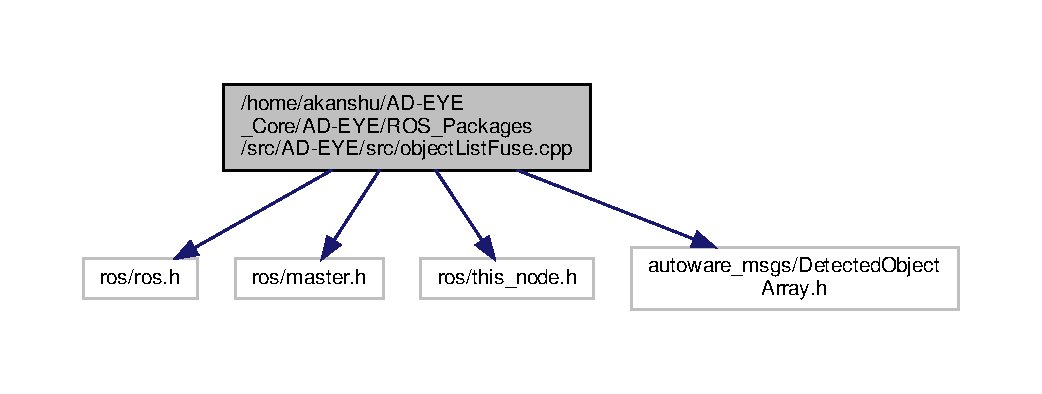
\includegraphics[width=350pt]{objectListFuse_8cpp__incl}
\end{center}
\end{figure}
\subsection*{Classes}
\begin{DoxyCompactItemize}
\item 
class \hyperlink{classobjectListFuse}{object\+List\+Fuse}
\end{DoxyCompactItemize}
\subsection*{Functions}
\begin{DoxyCompactItemize}
\item 
void \hyperlink{objectListFuse_8cpp_aa89874c10460404be51a149466355178}{usage} (std\+::string bin\+Name)
\item 
int \hyperlink{objectListFuse_8cpp_a3c04138a5bfe5d72780bb7e82a18e627}{main} (int argc, char $\ast$$\ast$argv)
\end{DoxyCompactItemize}


\subsection{Function Documentation}
\mbox{\Hypertarget{objectListFuse_8cpp_a3c04138a5bfe5d72780bb7e82a18e627}\label{objectListFuse_8cpp_a3c04138a5bfe5d72780bb7e82a18e627}} 
\index{object\+List\+Fuse.\+cpp@{object\+List\+Fuse.\+cpp}!main@{main}}
\index{main@{main}!object\+List\+Fuse.\+cpp@{object\+List\+Fuse.\+cpp}}
\subsubsection{\texorpdfstring{main()}{main()}}
{\footnotesize\ttfamily int main (\begin{DoxyParamCaption}\item[{int}]{argc,  }\item[{char $\ast$$\ast$}]{argv }\end{DoxyParamCaption})}

\mbox{\Hypertarget{objectListFuse_8cpp_aa89874c10460404be51a149466355178}\label{objectListFuse_8cpp_aa89874c10460404be51a149466355178}} 
\index{object\+List\+Fuse.\+cpp@{object\+List\+Fuse.\+cpp}!usage@{usage}}
\index{usage@{usage}!object\+List\+Fuse.\+cpp@{object\+List\+Fuse.\+cpp}}
\subsubsection{\texorpdfstring{usage()}{usage()}}
{\footnotesize\ttfamily void usage (\begin{DoxyParamCaption}\item[{std\+::string}]{bin\+Name }\end{DoxyParamCaption})}


\hypertarget{objectsFrameAdapter_8cpp}{}\section{/home/akanshu/\+A\+D-\/\+E\+Y\+E\+\_\+\+Core/\+A\+D-\/\+E\+Y\+E/\+R\+O\+S\+\_\+\+Packages/src/\+A\+D-\/\+E\+Y\+E/src/objects\+Frame\+Adapter.cpp File Reference}
\label{objectsFrameAdapter_8cpp}\index{/home/akanshu/\+A\+D-\/\+E\+Y\+E\+\_\+\+Core/\+A\+D-\/\+E\+Y\+E/\+R\+O\+S\+\_\+\+Packages/src/\+A\+D-\/\+E\+Y\+E/src/objects\+Frame\+Adapter.\+cpp@{/home/akanshu/\+A\+D-\/\+E\+Y\+E\+\_\+\+Core/\+A\+D-\/\+E\+Y\+E/\+R\+O\+S\+\_\+\+Packages/src/\+A\+D-\/\+E\+Y\+E/src/objects\+Frame\+Adapter.\+cpp}}
{\ttfamily \#include $<$ros/ros.\+h$>$}\newline
{\ttfamily \#include $<$ros/master.\+h$>$}\newline
{\ttfamily \#include $<$ros/this\+\_\+node.\+h$>$}\newline
{\ttfamily \#include $<$autoware\+\_\+msgs/\+Detected\+Object\+Array.\+h$>$}\newline
{\ttfamily \#include $<$tf2\+\_\+ros/transform\+\_\+listener.\+h$>$}\newline
{\ttfamily \#include $<$geometry\+\_\+msgs/\+Transform\+Stamped.\+h$>$}\newline
{\ttfamily \#include $<$geometry\+\_\+msgs/\+Pose\+Stamped.\+h$>$}\newline
{\ttfamily \#include $<$geometry\+\_\+msgs/\+Point\+Stamped.\+h$>$}\newline
{\ttfamily \#include \char`\"{}tf2\+\_\+geometry\+\_\+msgs/tf2\+\_\+geometry\+\_\+msgs.\+h\char`\"{}}\newline
Include dependency graph for objects\+Frame\+Adapter.\+cpp\+:\nopagebreak
\begin{figure}[H]
\begin{center}
\leavevmode
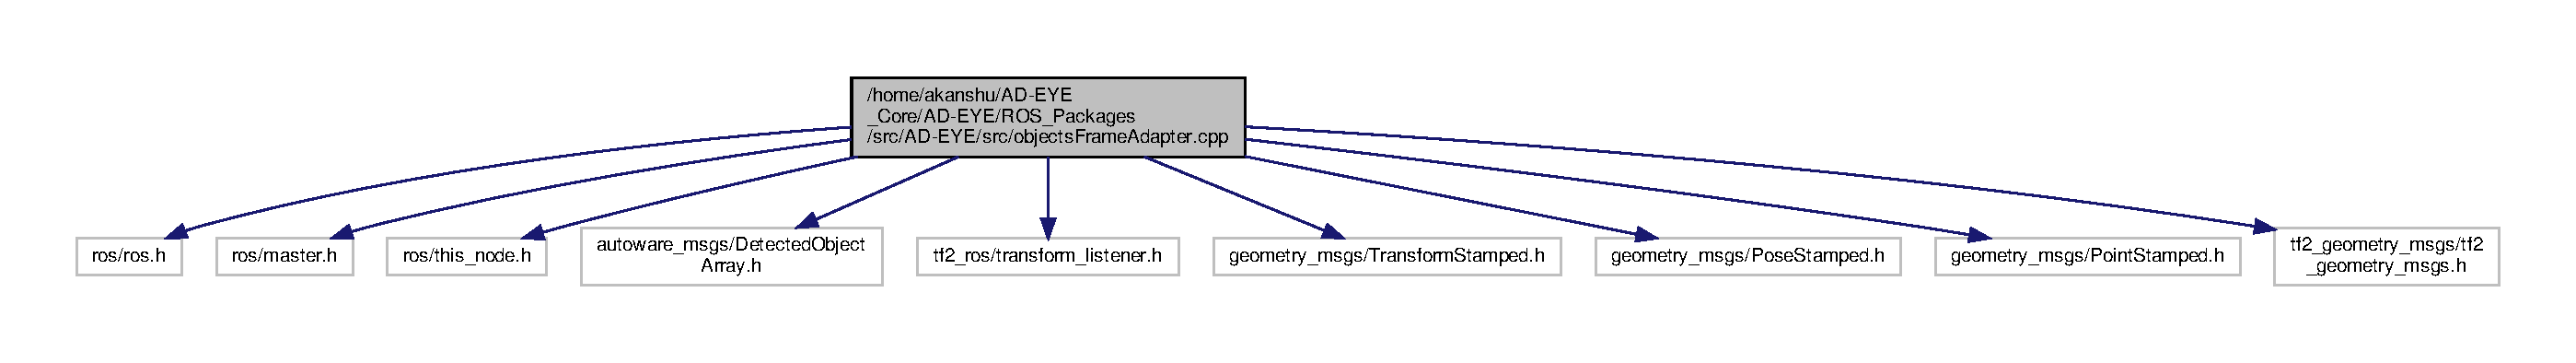
\includegraphics[width=350pt]{objectsFrameAdapter_8cpp__incl}
\end{center}
\end{figure}
\subsection*{Classes}
\begin{DoxyCompactItemize}
\item 
class \hyperlink{classobjectsFrameAdapter}{objects\+Frame\+Adapter}
\end{DoxyCompactItemize}
\subsection*{Functions}
\begin{DoxyCompactItemize}
\item 
void \hyperlink{objectsFrameAdapter_8cpp_aa89874c10460404be51a149466355178}{usage} (std\+::string bin\+Name)
\item 
int \hyperlink{objectsFrameAdapter_8cpp_a3c04138a5bfe5d72780bb7e82a18e627}{main} (int argc, char $\ast$$\ast$argv)
\end{DoxyCompactItemize}


\subsection{Function Documentation}
\mbox{\Hypertarget{objectsFrameAdapter_8cpp_a3c04138a5bfe5d72780bb7e82a18e627}\label{objectsFrameAdapter_8cpp_a3c04138a5bfe5d72780bb7e82a18e627}} 
\index{objects\+Frame\+Adapter.\+cpp@{objects\+Frame\+Adapter.\+cpp}!main@{main}}
\index{main@{main}!objects\+Frame\+Adapter.\+cpp@{objects\+Frame\+Adapter.\+cpp}}
\subsubsection{\texorpdfstring{main()}{main()}}
{\footnotesize\ttfamily int main (\begin{DoxyParamCaption}\item[{int}]{argc,  }\item[{char $\ast$$\ast$}]{argv }\end{DoxyParamCaption})}

\mbox{\Hypertarget{objectsFrameAdapter_8cpp_aa89874c10460404be51a149466355178}\label{objectsFrameAdapter_8cpp_aa89874c10460404be51a149466355178}} 
\index{objects\+Frame\+Adapter.\+cpp@{objects\+Frame\+Adapter.\+cpp}!usage@{usage}}
\index{usage@{usage}!objects\+Frame\+Adapter.\+cpp@{objects\+Frame\+Adapter.\+cpp}}
\subsubsection{\texorpdfstring{usage()}{usage()}}
{\footnotesize\ttfamily void usage (\begin{DoxyParamCaption}\item[{std\+::string}]{bin\+Name }\end{DoxyParamCaption})}


\hypertarget{point__cloud__receiver_8py}{}\section{/home/akanshu/\+A\+D-\/\+E\+Y\+E\+\_\+\+Core/\+A\+D-\/\+E\+Y\+E/\+R\+O\+S\+\_\+\+Packages/src/\+A\+D-\/\+E\+Y\+E/src/point\+\_\+cloud\+\_\+receiver.py File Reference}
\label{point__cloud__receiver_8py}\index{/home/akanshu/\+A\+D-\/\+E\+Y\+E\+\_\+\+Core/\+A\+D-\/\+E\+Y\+E/\+R\+O\+S\+\_\+\+Packages/src/\+A\+D-\/\+E\+Y\+E/src/point\+\_\+cloud\+\_\+receiver.\+py@{/home/akanshu/\+A\+D-\/\+E\+Y\+E\+\_\+\+Core/\+A\+D-\/\+E\+Y\+E/\+R\+O\+S\+\_\+\+Packages/src/\+A\+D-\/\+E\+Y\+E/src/point\+\_\+cloud\+\_\+receiver.\+py}}
\subsection*{Namespaces}
\begin{DoxyCompactItemize}
\item 
 \hyperlink{namespacepoint__cloud__receiver}{point\+\_\+cloud\+\_\+receiver}
\end{DoxyCompactItemize}
\subsection*{Functions}
\begin{DoxyCompactItemize}
\item 
def \hyperlink{namespacepoint__cloud__receiver_ae1f4d09e83639f1c6cc5c6a01e5c93c7}{point\+\_\+cloud\+\_\+receiver.\+mycallback} (data)
\end{DoxyCompactItemize}
\subsection*{Variables}
\begin{DoxyCompactItemize}
\item 
\hyperlink{namespacepoint__cloud__receiver_a24216fb78df876244247dbd01fa04733}{point\+\_\+cloud\+\_\+receiver.\+anonymous}
\item 
\hyperlink{namespacepoint__cloud__receiver_a02fb03398de59f401d26b98cec00eaab}{point\+\_\+cloud\+\_\+receiver.\+pub} = rospy.\+Publisher(\textquotesingle{}/points\+\_\+raw\textquotesingle{}, Point\+Cloud2, queue\+\_\+size=1)
\end{DoxyCompactItemize}

\hypertarget{radar__broadcaster_8cpp}{}\section{/home/akanshu/\+A\+D-\/\+E\+Y\+E\+\_\+\+Core/\+A\+D-\/\+E\+Y\+E/\+R\+O\+S\+\_\+\+Packages/src/\+A\+D-\/\+E\+Y\+E/src/radar\+\_\+broadcaster.cpp File Reference}
\label{radar__broadcaster_8cpp}\index{/home/akanshu/\+A\+D-\/\+E\+Y\+E\+\_\+\+Core/\+A\+D-\/\+E\+Y\+E/\+R\+O\+S\+\_\+\+Packages/src/\+A\+D-\/\+E\+Y\+E/src/radar\+\_\+broadcaster.\+cpp@{/home/akanshu/\+A\+D-\/\+E\+Y\+E\+\_\+\+Core/\+A\+D-\/\+E\+Y\+E/\+R\+O\+S\+\_\+\+Packages/src/\+A\+D-\/\+E\+Y\+E/src/radar\+\_\+broadcaster.\+cpp}}
{\ttfamily \#include $<$ros/ros.\+h$>$}\newline
{\ttfamily \#include $<$ros/master.\+h$>$}\newline
{\ttfamily \#include $<$ros/this\+\_\+node.\+h$>$}\newline
{\ttfamily \#include $<$std\+\_\+msgs/\+Float32\+Multi\+Array.\+h$>$}\newline
{\ttfamily \#include $<$autoware\+\_\+msgs/\+Detected\+Object.\+h$>$}\newline
{\ttfamily \#include $<$autoware\+\_\+msgs/\+Detected\+Object\+Array.\+h$>$}\newline
{\ttfamily \#include $<$geometry\+\_\+msgs/\+Point32.\+h$>$}\newline
Include dependency graph for radar\+\_\+broadcaster.\+cpp\+:\nopagebreak
\begin{figure}[H]
\begin{center}
\leavevmode
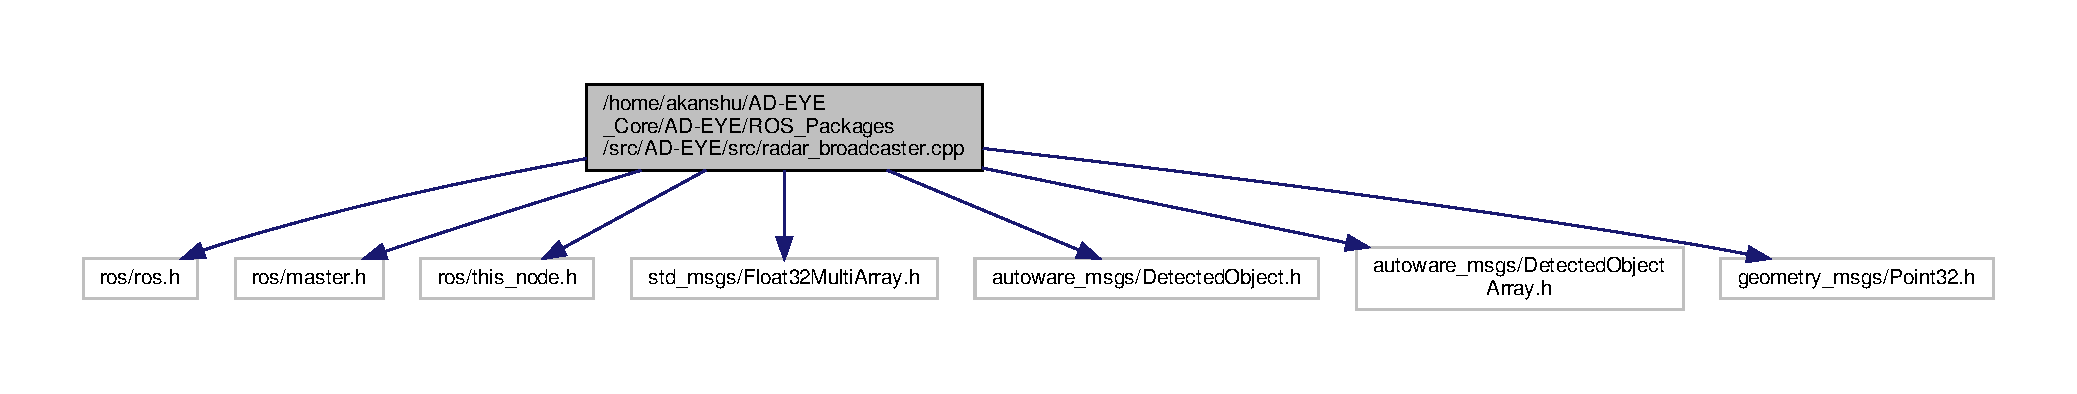
\includegraphics[width=350pt]{radar__broadcaster_8cpp__incl}
\end{center}
\end{figure}
\subsection*{Classes}
\begin{DoxyCompactItemize}
\item 
class \hyperlink{classradarBroadcaster}{radar\+Broadcaster}
\end{DoxyCompactItemize}
\subsection*{Functions}
\begin{DoxyCompactItemize}
\item 
int \hyperlink{radar__broadcaster_8cpp_a3c04138a5bfe5d72780bb7e82a18e627}{main} (int argc, char $\ast$$\ast$argv)
\end{DoxyCompactItemize}


\subsection{Function Documentation}
\mbox{\Hypertarget{radar__broadcaster_8cpp_a3c04138a5bfe5d72780bb7e82a18e627}\label{radar__broadcaster_8cpp_a3c04138a5bfe5d72780bb7e82a18e627}} 
\index{radar\+\_\+broadcaster.\+cpp@{radar\+\_\+broadcaster.\+cpp}!main@{main}}
\index{main@{main}!radar\+\_\+broadcaster.\+cpp@{radar\+\_\+broadcaster.\+cpp}}
\subsubsection{\texorpdfstring{main()}{main()}}
{\footnotesize\ttfamily int main (\begin{DoxyParamCaption}\item[{int}]{argc,  }\item[{char $\ast$$\ast$}]{argv }\end{DoxyParamCaption})}


\hypertarget{rp__manager_8py}{}\section{/home/akanshu/\+A\+D-\/\+E\+Y\+E\+\_\+\+Core/\+A\+D-\/\+E\+Y\+E/\+R\+O\+S\+\_\+\+Packages/src/\+A\+D-\/\+E\+Y\+E/src/rp\+\_\+manager.py File Reference}
\label{rp__manager_8py}\index{/home/akanshu/\+A\+D-\/\+E\+Y\+E\+\_\+\+Core/\+A\+D-\/\+E\+Y\+E/\+R\+O\+S\+\_\+\+Packages/src/\+A\+D-\/\+E\+Y\+E/src/rp\+\_\+manager.\+py@{/home/akanshu/\+A\+D-\/\+E\+Y\+E\+\_\+\+Core/\+A\+D-\/\+E\+Y\+E/\+R\+O\+S\+\_\+\+Packages/src/\+A\+D-\/\+E\+Y\+E/src/rp\+\_\+manager.\+py}}
\subsection*{Namespaces}
\begin{DoxyCompactItemize}
\item 
 \hyperlink{namespacerp__manager}{rp\+\_\+manager}
\end{DoxyCompactItemize}
\subsection*{Functions}
\begin{DoxyCompactItemize}
\item 
def \hyperlink{namespacerp__manager_a12d1e048fb6f0fcabb8e81c26f042ed5}{rp\+\_\+manager.\+simulink\+\_\+state\+\_\+callback} (msg)
\end{DoxyCompactItemize}
\subsection*{Variables}
\begin{DoxyCompactItemize}
\item 
int \hyperlink{namespacerp__manager_ad9b2dec1c2adc525d94b09f0505b041c}{rp\+\_\+manager.\+E\+N\+A\+B\+L\+ED} = 1
\item 
int \hyperlink{namespacerp__manager_af85e17f72f768eba5168eba56041bd69}{rp\+\_\+manager.\+D\+I\+S\+A\+B\+L\+ED} = 0
\item 
list \hyperlink{namespacerp__manager_a72ed7a08fe7d40ac96ae84a2f15d504f}{rp\+\_\+manager.\+F\+E\+A\+T\+U\+R\+E\+\_\+\+E\+N\+A\+B\+L\+ED} = \mbox{[}True for i in range(9)\mbox{]}
\item 
int \hyperlink{namespacerp__manager_a68068aeea47c1d38c09708b72d400462}{rp\+\_\+manager.\+R\+V\+IZ} = 1
\item 
int \hyperlink{namespacerp__manager_acbff7b63b4d20bf93d9281425037cef9}{rp\+\_\+manager.\+M\+A\+P\+P\+I\+NG} = 2
\item 
int \hyperlink{namespacerp__manager_a50a8ef40ff1b66406cc44a08b34a8289}{rp\+\_\+manager.\+L\+O\+C\+A\+L\+I\+Z\+A\+T\+I\+ON} = 3
\item 
int \hyperlink{namespacerp__manager_a3e3537ea325816427b2b1289f0c80ad6}{rp\+\_\+manager.\+S\+E\+N\+S\+I\+NG} = 4
\item 
int \hyperlink{namespacerp__manager_ac227be112745c88525a9667580cec00b}{rp\+\_\+manager.\+D\+E\+T\+E\+C\+T\+I\+ON} = 5
\item 
int \hyperlink{namespacerp__manager_a1638954fddcfcecdb0f5ea6dcaeb349e}{rp\+\_\+manager.\+S\+W\+I\+T\+CH} = 6
\item 
int \hyperlink{namespacerp__manager_a02a3da6c0c6f1434866a0e755a91b611}{rp\+\_\+manager.\+M\+I\+S\+S\+I\+O\+N\+\_\+\+P\+L\+A\+N\+N\+I\+NG} = 7
\item 
int \hyperlink{namespacerp__manager_a82d79fb07692d1357006f56f6d1b99da}{rp\+\_\+manager.\+M\+O\+T\+I\+O\+N\+\_\+\+P\+L\+A\+N\+N\+I\+NG} = 8
\item 
int \hyperlink{namespacerp__manager_afa43e98bce9dbb3e8c4ebddcae4e025d}{rp\+\_\+manager.\+S\+S\+MP} = 9
\item 
\hyperlink{namespacerp__manager_ae453dc601914cd184683c09184ce35c3}{rp\+\_\+manager.\+rospack} = rospkg.\+Ros\+Pack()
\item 
string \hyperlink{namespacerp__manager_a86043a0cf61411011e16931d9164b284}{rp\+\_\+manager.\+A\+D\+E\+Y\+E\+\_\+\+P\+A\+C\+K\+A\+G\+E\+\_\+\+L\+O\+C\+A\+T\+I\+ON} = rospack.\+get\+\_\+path(\textquotesingle{}adeye\textquotesingle{})+\char`\"{}/\char`\"{}
\item 
string \hyperlink{namespacerp__manager_a43208312336e22fa0f9a976a69e1519e}{rp\+\_\+manager.\+M\+O\+D\+I\+F\+I\+E\+D\+\_\+\+L\+A\+U\+N\+C\+H\+\_\+\+F\+I\+L\+E\+S\+\_\+\+L\+O\+C\+A\+T\+I\+ON} = \char`\"{}modified\+\_\+launch\+\_\+files/\char`\"{}
\item 
string \hyperlink{namespacerp__manager_af0ff9dba303cc42af7c94b91bd577a4f}{rp\+\_\+manager.\+L\+A\+U\+N\+C\+H\+\_\+\+F\+O\+L\+D\+E\+R\+\_\+\+L\+O\+C\+A\+T\+I\+ON} = \char`\"{}launch/\char`\"{}
\item 
string \hyperlink{namespacerp__manager_afed1d2027e1ae55feaab901b6ace615f}{rp\+\_\+manager.\+R\+V\+I\+Z\+\_\+\+L\+A\+U\+N\+C\+H\+\_\+\+F\+I\+L\+E\+\_\+\+N\+A\+ME} = \char`\"{}rp\+\_\+my\+\_\+rviz.\+launch\char`\"{}
\item 
string \hyperlink{namespacerp__manager_aac197302609510b15a932831ab9345f6}{rp\+\_\+manager.\+M\+A\+P\+P\+I\+N\+G\+\_\+\+L\+A\+U\+N\+C\+H\+\_\+\+F\+I\+L\+E\+\_\+\+N\+A\+ME} = \char`\"{}rp\+\_\+my\+\_\+map.\+launch\char`\"{}
\item 
string \hyperlink{namespacerp__manager_a6dcd95bd9477c77584799b731cf6e853}{rp\+\_\+manager.\+L\+O\+C\+A\+L\+I\+Z\+A\+T\+I\+O\+N\+\_\+\+L\+A\+U\+N\+C\+H\+\_\+\+F\+I\+L\+E\+\_\+\+N\+A\+ME} = \char`\"{}rp\+\_\+my\+\_\+localization.\+launch\char`\"{}
\item 
string \hyperlink{namespacerp__manager_ac4cd90df1f22dfc4387eb36bcfd8215c}{rp\+\_\+manager.\+F\+A\+K\+E\+\_\+\+L\+O\+C\+A\+L\+I\+Z\+A\+T\+I\+O\+N\+\_\+\+L\+A\+U\+N\+C\+H\+\_\+\+F\+I\+L\+E\+\_\+\+N\+A\+ME} = \char`\"{}rp\+\_\+my\+\_\+fake\+\_\+localization.\+launch\char`\"{}
\item 
string \hyperlink{namespacerp__manager_a4b5be1d16a3c9ba81e23daa96404fcaa}{rp\+\_\+manager.\+S\+E\+N\+S\+I\+N\+G\+\_\+\+L\+A\+U\+N\+C\+H\+\_\+\+F\+I\+L\+E\+\_\+\+N\+A\+ME} = \char`\"{}rp\+\_\+my\+\_\+sensing.\+launch\char`\"{}
\item 
string \hyperlink{namespacerp__manager_abf958196458f1890b8b9077998975e2e}{rp\+\_\+manager.\+D\+E\+T\+E\+C\+T\+I\+O\+N\+\_\+\+L\+A\+U\+N\+C\+H\+\_\+\+F\+I\+L\+E\+\_\+\+N\+A\+ME} = \char`\"{}rp\+\_\+my\+\_\+detection.\+launch\char`\"{}
\item 
string \hyperlink{namespacerp__manager_afa1029c78f6d8652ba47f268602aacf4}{rp\+\_\+manager.\+S\+W\+I\+T\+C\+H\+\_\+\+L\+A\+U\+N\+C\+H\+\_\+\+F\+I\+L\+E\+\_\+\+N\+A\+ME} = \char`\"{}switch.\+launch\char`\"{}
\item 
string \hyperlink{namespacerp__manager_a8385af25b9217972b5859c9bc28dcce2}{rp\+\_\+manager.\+M\+I\+S\+S\+I\+O\+N\+\_\+\+P\+L\+A\+N\+N\+I\+N\+G\+\_\+\+L\+A\+U\+N\+C\+H\+\_\+\+F\+I\+L\+E\+\_\+\+N\+A\+ME} = \char`\"{}rp\+\_\+my\+\_\+mission\+\_\+planning.\+launch\char`\"{}
\item 
string \hyperlink{namespacerp__manager_ad8005b248e4af4a6127f9aaf678f7447}{rp\+\_\+manager.\+M\+O\+T\+I\+O\+N\+\_\+\+P\+L\+A\+N\+N\+I\+N\+G\+\_\+\+L\+A\+U\+N\+C\+H\+\_\+\+F\+I\+L\+E\+\_\+\+N\+A\+ME} = \char`\"{}rp\+\_\+my\+\_\+motion\+\_\+planning.\+launch\char`\"{}
\item 
string \hyperlink{namespacerp__manager_addd21ac261b0a72d27fa7b982ba438c6}{rp\+\_\+manager.\+S\+S\+M\+P\+\_\+\+L\+A\+U\+N\+C\+H\+\_\+\+F\+I\+L\+E\+\_\+\+N\+A\+ME} = \char`\"{}rp\+\_\+\+S\+S\+M\+P.\+launch\char`\"{}
\item 
tuple \hyperlink{namespacerp__manager_a4b6881a6710271456550e946aa632115}{rp\+\_\+manager.\+R\+V\+I\+Z\+\_\+\+F\+U\+L\+L\+\_\+\+P\+A\+TH} = (\char`\"{}\%s\%s\%s\char`\"{} \% (A\+D\+E\+Y\+E\+\_\+\+P\+A\+C\+K\+A\+G\+E\+\_\+\+L\+O\+C\+A\+T\+I\+ON, M\+O\+D\+I\+F\+I\+E\+D\+\_\+\+L\+A\+U\+N\+C\+H\+\_\+\+F\+I\+L\+E\+S\+\_\+\+L\+O\+C\+A\+T\+I\+ON, R\+V\+I\+Z\+\_\+\+L\+A\+U\+N\+C\+H\+\_\+\+F\+I\+L\+E\+\_\+\+N\+A\+ME))
\item 
tuple \hyperlink{namespacerp__manager_af7dfe82383bf37c2c7990a430fd30ae2}{rp\+\_\+manager.\+M\+A\+P\+P\+I\+N\+G\+\_\+\+F\+U\+L\+L\+\_\+\+P\+A\+TH} = (\char`\"{}\%s\%s\%s\char`\"{} \% (A\+D\+E\+Y\+E\+\_\+\+P\+A\+C\+K\+A\+G\+E\+\_\+\+L\+O\+C\+A\+T\+I\+ON, M\+O\+D\+I\+F\+I\+E\+D\+\_\+\+L\+A\+U\+N\+C\+H\+\_\+\+F\+I\+L\+E\+S\+\_\+\+L\+O\+C\+A\+T\+I\+ON, M\+A\+P\+P\+I\+N\+G\+\_\+\+L\+A\+U\+N\+C\+H\+\_\+\+F\+I\+L\+E\+\_\+\+N\+A\+ME))
\item 
tuple \hyperlink{namespacerp__manager_a34400d772701b08f8c9a99692b4c3a0e}{rp\+\_\+manager.\+L\+O\+C\+A\+L\+I\+Z\+A\+T\+I\+O\+N\+\_\+\+F\+U\+L\+L\+\_\+\+P\+A\+TH} = (\char`\"{}\%s\%s\%s\char`\"{} \% (A\+D\+E\+Y\+E\+\_\+\+P\+A\+C\+K\+A\+G\+E\+\_\+\+L\+O\+C\+A\+T\+I\+ON, M\+O\+D\+I\+F\+I\+E\+D\+\_\+\+L\+A\+U\+N\+C\+H\+\_\+\+F\+I\+L\+E\+S\+\_\+\+L\+O\+C\+A\+T\+I\+ON, L\+O\+C\+A\+L\+I\+Z\+A\+T\+I\+O\+N\+\_\+\+L\+A\+U\+N\+C\+H\+\_\+\+F\+I\+L\+E\+\_\+\+N\+A\+ME))
\item 
tuple \hyperlink{namespacerp__manager_ad7b467e777f8d6cdf79d68ac4e2cf01b}{rp\+\_\+manager.\+F\+A\+K\+E\+\_\+\+L\+O\+C\+A\+L\+I\+Z\+A\+T\+I\+O\+N\+\_\+\+F\+U\+L\+L\+\_\+\+P\+A\+TH} = (\char`\"{}\%s\%s\%s\char`\"{} \% (A\+D\+E\+Y\+E\+\_\+\+P\+A\+C\+K\+A\+G\+E\+\_\+\+L\+O\+C\+A\+T\+I\+ON, M\+O\+D\+I\+F\+I\+E\+D\+\_\+\+L\+A\+U\+N\+C\+H\+\_\+\+F\+I\+L\+E\+S\+\_\+\+L\+O\+C\+A\+T\+I\+ON, F\+A\+K\+E\+\_\+\+L\+O\+C\+A\+L\+I\+Z\+A\+T\+I\+O\+N\+\_\+\+L\+A\+U\+N\+C\+H\+\_\+\+F\+I\+L\+E\+\_\+\+N\+A\+ME))
\item 
tuple \hyperlink{namespacerp__manager_af912fb7c706707b4b2a06ba4cf4a5d24}{rp\+\_\+manager.\+S\+E\+N\+S\+I\+N\+G\+\_\+\+F\+U\+L\+L\+\_\+\+P\+A\+TH} = (\char`\"{}\%s\%s\%s\char`\"{} \% (A\+D\+E\+Y\+E\+\_\+\+P\+A\+C\+K\+A\+G\+E\+\_\+\+L\+O\+C\+A\+T\+I\+ON, M\+O\+D\+I\+F\+I\+E\+D\+\_\+\+L\+A\+U\+N\+C\+H\+\_\+\+F\+I\+L\+E\+S\+\_\+\+L\+O\+C\+A\+T\+I\+ON, S\+E\+N\+S\+I\+N\+G\+\_\+\+L\+A\+U\+N\+C\+H\+\_\+\+F\+I\+L\+E\+\_\+\+N\+A\+ME))
\item 
tuple \hyperlink{namespacerp__manager_a70fad5203ba45cd0085ee33158b164be}{rp\+\_\+manager.\+D\+E\+T\+E\+C\+T\+I\+O\+N\+\_\+\+F\+U\+L\+L\+\_\+\+P\+A\+TH} = (\char`\"{}\%s\%s\%s\char`\"{} \% (A\+D\+E\+Y\+E\+\_\+\+P\+A\+C\+K\+A\+G\+E\+\_\+\+L\+O\+C\+A\+T\+I\+ON, M\+O\+D\+I\+F\+I\+E\+D\+\_\+\+L\+A\+U\+N\+C\+H\+\_\+\+F\+I\+L\+E\+S\+\_\+\+L\+O\+C\+A\+T\+I\+ON, D\+E\+T\+E\+C\+T\+I\+O\+N\+\_\+\+L\+A\+U\+N\+C\+H\+\_\+\+F\+I\+L\+E\+\_\+\+N\+A\+ME))
\item 
tuple \hyperlink{namespacerp__manager_a98789269c0bde80d85d5c62af5133062}{rp\+\_\+manager.\+S\+W\+I\+T\+C\+H\+\_\+\+F\+U\+L\+L\+\_\+\+P\+A\+TH} = (\char`\"{}\%s\%s\%s\char`\"{} \% (A\+D\+E\+Y\+E\+\_\+\+P\+A\+C\+K\+A\+G\+E\+\_\+\+L\+O\+C\+A\+T\+I\+ON, L\+A\+U\+N\+C\+H\+\_\+\+F\+O\+L\+D\+E\+R\+\_\+\+L\+O\+C\+A\+T\+I\+ON, S\+W\+I\+T\+C\+H\+\_\+\+L\+A\+U\+N\+C\+H\+\_\+\+F\+I\+L\+E\+\_\+\+N\+A\+ME))
\item 
tuple \hyperlink{namespacerp__manager_a09c2ace0ccdb1ed70e1cb0b1a8997367}{rp\+\_\+manager.\+M\+I\+S\+S\+I\+O\+N\+\_\+\+P\+L\+A\+N\+N\+I\+N\+G\+\_\+\+F\+U\+L\+L\+\_\+\+P\+A\+TH}
\item 
tuple \hyperlink{namespacerp__manager_abfcfbb274df96ce74ae7f446c5a23763}{rp\+\_\+manager.\+M\+O\+T\+I\+O\+N\+\_\+\+P\+L\+A\+N\+N\+I\+N\+G\+\_\+\+F\+U\+L\+L\+\_\+\+P\+A\+TH}
\item 
tuple \hyperlink{namespacerp__manager_aa5f54d7effc05602e428d9d5829184c9}{rp\+\_\+manager.\+S\+S\+M\+P\+\_\+\+F\+U\+L\+L\+\_\+\+P\+A\+TH} = (\char`\"{}\%s\%s\%s\char`\"{} \% (A\+D\+E\+Y\+E\+\_\+\+P\+A\+C\+K\+A\+G\+E\+\_\+\+L\+O\+C\+A\+T\+I\+ON, M\+O\+D\+I\+F\+I\+E\+D\+\_\+\+L\+A\+U\+N\+C\+H\+\_\+\+F\+I\+L\+E\+S\+\_\+\+L\+O\+C\+A\+T\+I\+ON, S\+S\+M\+P\+\_\+\+L\+A\+U\+N\+C\+H\+\_\+\+F\+I\+L\+E\+\_\+\+N\+A\+ME))
\item 
int \hyperlink{namespacerp__manager_ae777617cb6dd55d3254cf75c4cdfbfd5}{rp\+\_\+manager.\+M\+A\+P\+P\+I\+N\+G\+\_\+\+S\+T\+A\+R\+T\+\_\+\+W\+A\+I\+T\+\_\+\+T\+I\+ME} = 10
\item 
int \hyperlink{namespacerp__manager_adc40cec510857cc5bb8413424beac186}{rp\+\_\+manager.\+L\+O\+C\+A\+L\+I\+Z\+A\+T\+I\+O\+N\+\_\+\+S\+T\+A\+R\+T\+\_\+\+W\+A\+I\+T\+\_\+\+T\+I\+ME} = 10
\item 
int \hyperlink{namespacerp__manager_a38b9eb0e03b90a19ad2a9f3cbac93eba}{rp\+\_\+manager.\+L\+O\+C\+A\+L\+I\+Z\+A\+T\+I\+O\+N\+\_\+\+S\+T\+O\+P\+\_\+\+W\+A\+I\+T\+\_\+\+T\+I\+ME} = 10
\item 
int \hyperlink{namespacerp__manager_a2a1de6661f1541719bab9d3d2e7661a1}{rp\+\_\+manager.\+D\+E\+T\+E\+C\+T\+I\+O\+N\+\_\+\+S\+T\+O\+P\+\_\+\+W\+A\+I\+T\+\_\+\+T\+I\+ME} = 10
\item 
int \hyperlink{namespacerp__manager_a03431ff00baee9003b9897bcfb5e05ca}{rp\+\_\+manager.\+M\+I\+S\+S\+I\+O\+N\+\_\+\+P\+L\+A\+N\+N\+I\+N\+G\+\_\+\+S\+T\+A\+R\+T\+\_\+\+W\+A\+I\+T\+\_\+\+T\+I\+ME} = 5
\item 
int \hyperlink{namespacerp__manager_a4aedafb6426407e86b472aba3711903d}{rp\+\_\+manager.\+M\+I\+S\+S\+I\+O\+N\+\_\+\+P\+L\+A\+N\+N\+I\+N\+G\+\_\+\+S\+T\+O\+P\+\_\+\+W\+A\+I\+T\+\_\+\+T\+I\+ME} = 10
\item 
int \hyperlink{namespacerp__manager_af8fe99e675b5d549f9b6b93de26c41f5}{rp\+\_\+manager.\+M\+O\+T\+I\+O\+N\+\_\+\+P\+L\+A\+N\+N\+I\+N\+G\+\_\+\+S\+T\+O\+P\+\_\+\+W\+A\+I\+T\+\_\+\+T\+I\+ME} = 10
\item 
list \hyperlink{namespacerp__manager_a5071f53ee23fdca3994006206cbcf2ee}{rp\+\_\+manager.\+previous\+\_\+simulink\+\_\+state} = \mbox{[}D\+I\+S\+A\+B\+L\+ED, D\+I\+S\+A\+B\+L\+ED, D\+I\+S\+A\+B\+L\+ED, D\+I\+S\+A\+B\+L\+ED, D\+I\+S\+A\+B\+L\+ED, D\+I\+S\+A\+B\+L\+ED, D\+I\+S\+A\+B\+L\+ED, D\+I\+S\+A\+B\+L\+ED, D\+I\+S\+A\+B\+L\+ED, D\+I\+S\+A\+B\+L\+ED\mbox{]}
\item 
list \hyperlink{namespacerp__manager_a85cdd1b22b56bd5cc90234794b44872c}{rp\+\_\+manager.\+current\+\_\+simulink\+\_\+state} = \mbox{[}D\+I\+S\+A\+B\+L\+ED, D\+I\+S\+A\+B\+L\+ED, D\+I\+S\+A\+B\+L\+ED, D\+I\+S\+A\+B\+L\+ED, D\+I\+S\+A\+B\+L\+ED, D\+I\+S\+A\+B\+L\+ED, D\+I\+S\+A\+B\+L\+ED, D\+I\+S\+A\+B\+L\+ED, D\+I\+S\+A\+B\+L\+ED, D\+I\+S\+A\+B\+L\+ED\mbox{]}
\item 
bool \hyperlink{namespacerp__manager_a4eb11cbe8e6db21cbbf9855db440635c}{rp\+\_\+manager.\+point\+\_\+map\+\_\+ready} = False
\item 
\hyperlink{namespacerp__manager_af20e1a3af6f948381fd6cf62eea8428d}{rp\+\_\+manager.\+Rviz} = Feature\+Control(R\+V\+I\+Z\+\_\+\+F\+U\+L\+L\+\_\+\+P\+A\+TH, \char`\"{}Rviz\char`\"{})
\item 
\hyperlink{namespacerp__manager_a09e73c9af6b8dae0a30b9137bf64f78c}{rp\+\_\+manager.\+Mapping} = Feature\+Control(M\+A\+P\+P\+I\+N\+G\+\_\+\+F\+U\+L\+L\+\_\+\+P\+A\+TH, \char`\"{}Mapping\char`\"{}, M\+A\+P\+P\+I\+N\+G\+\_\+\+S\+T\+A\+R\+T\+\_\+\+W\+A\+I\+T\+\_\+\+T\+I\+ME)
\item 
\hyperlink{namespacerp__manager_a96726b99cc68f4ab799319275c9d15c8}{rp\+\_\+manager.\+Sensing} = Feature\+Control(S\+E\+N\+S\+I\+N\+G\+\_\+\+F\+U\+L\+L\+\_\+\+P\+A\+TH, \char`\"{}Sensing\char`\"{})
\item 
\hyperlink{namespacerp__manager_a74726f38318729f38449240240efaae5}{rp\+\_\+manager.\+Localization}
\item 
\hyperlink{namespacerp__manager_a67b92cded2b796d9f50a73c53191dfd5}{rp\+\_\+manager.\+Fake\+\_\+\+Localization} = Feature\+Control(F\+A\+K\+E\+\_\+\+L\+O\+C\+A\+L\+I\+Z\+A\+T\+I\+O\+N\+\_\+\+F\+U\+L\+L\+\_\+\+P\+A\+TH, \char`\"{}Fake\+\_\+\+Localization\char`\"{})
\item 
\hyperlink{namespacerp__manager_a48713c04a94d14edf4a48051376c73ca}{rp\+\_\+manager.\+Detection} = Feature\+Control(D\+E\+T\+E\+C\+T\+I\+O\+N\+\_\+\+F\+U\+L\+L\+\_\+\+P\+A\+TH, \char`\"{}Detection\char`\"{}, sleep\+\_\+time\+\_\+on\+\_\+stop=D\+E\+T\+E\+C\+T\+I\+O\+N\+\_\+\+S\+T\+O\+P\+\_\+\+W\+A\+I\+T\+\_\+\+T\+I\+ME)
\item 
\hyperlink{namespacerp__manager_a13a981f0dfd4007cc0341452cc0696ee}{rp\+\_\+manager.\+Mission\+\_\+planning}
\item 
\hyperlink{namespacerp__manager_a1ea58b084aa5c6382085b94b09a107f5}{rp\+\_\+manager.\+Motion\+\_\+planning}
\item 
\hyperlink{namespacerp__manager_ae41df772e3f2842aea416ed2b6f26ec0}{rp\+\_\+manager.\+Switch} = Feature\+Control(S\+W\+I\+T\+C\+H\+\_\+\+F\+U\+L\+L\+\_\+\+P\+A\+TH, \char`\"{}Switch\char`\"{})
\item 
\hyperlink{namespacerp__manager_a526a1df0e334b5e0026a6d4f4d851195}{rp\+\_\+manager.\+Ssmp} = Feature\+Control(S\+S\+M\+P\+\_\+\+F\+U\+L\+L\+\_\+\+P\+A\+TH, \char`\"{}S\+S\+MP\char`\"{})
\item 
\hyperlink{namespacerp__manager_a356ae7e0a3da8c3f6d968b297f09cf8a}{rp\+\_\+manager.\+rate} = rospy.\+Rate(10.\+0)
\end{DoxyCompactItemize}

\hypertarget{safetySupervisor_8cpp}{}\section{/home/akanshu/\+A\+D-\/\+E\+Y\+E\+\_\+\+Core/\+A\+D-\/\+E\+Y\+E/\+R\+O\+S\+\_\+\+Packages/src/\+A\+D-\/\+E\+Y\+E/src/safety\+Supervisor.cpp File Reference}
\label{safetySupervisor_8cpp}\index{/home/akanshu/\+A\+D-\/\+E\+Y\+E\+\_\+\+Core/\+A\+D-\/\+E\+Y\+E/\+R\+O\+S\+\_\+\+Packages/src/\+A\+D-\/\+E\+Y\+E/src/safety\+Supervisor.\+cpp@{/home/akanshu/\+A\+D-\/\+E\+Y\+E\+\_\+\+Core/\+A\+D-\/\+E\+Y\+E/\+R\+O\+S\+\_\+\+Packages/src/\+A\+D-\/\+E\+Y\+E/src/safety\+Supervisor.\+cpp}}
{\ttfamily \#include $<$ros/ros.\+h$>$}\newline
{\ttfamily \#include $<$ros/master.\+h$>$}\newline
{\ttfamily \#include $<$ros/this\+\_\+node.\+h$>$}\newline
{\ttfamily \#include $<$grid\+\_\+map\+\_\+ros/grid\+\_\+map\+\_\+ros.\+hpp$>$}\newline
{\ttfamily \#include $<$grid\+\_\+map\+\_\+msgs/\+Grid\+Map.\+h$>$}\newline
{\ttfamily \#include $<$geometry\+\_\+msgs/\+Pose\+Stamped.\+h$>$}\newline
{\ttfamily \#include $<$geometry\+\_\+msgs/\+Pose.\+h$>$}\newline
{\ttfamily \#include $<$std\+\_\+msgs/\+Int32.\+h$>$}\newline
{\ttfamily \#include $<$std\+\_\+msgs/\+Float32\+Multi\+Array.\+h$>$}\newline
{\ttfamily \#include $<$std\+\_\+msgs/\+Float32.\+h$>$}\newline
{\ttfamily \#include $<$autoware\+\_\+msgs/\+Lane.\+h$>$}\newline
{\ttfamily \#include $<$autoware\+\_\+msgs/\+Lane\+Array.\+h$>$}\newline
{\ttfamily \#include $<$cpp\+\_\+utils/pose\+\_\+datatypes.\+h$>$}\newline
{\ttfamily \#include $<$visualization\+\_\+msgs/\+Marker.\+h$>$}\newline
{\ttfamily \#include $<$std\+\_\+msgs/\+Color\+R\+G\+B\+A.\+h$>$}\newline
{\ttfamily \#include \char`\"{}op\+\_\+planner/\+Planner\+H.\+h\char`\"{}}\newline
{\ttfamily \#include \char`\"{}op\+\_\+ros\+\_\+helpers/op\+\_\+\+R\+O\+S\+Helpers.\+h\char`\"{}}\newline
Include dependency graph for safety\+Supervisor.\+cpp\+:\nopagebreak
\begin{figure}[H]
\begin{center}
\leavevmode
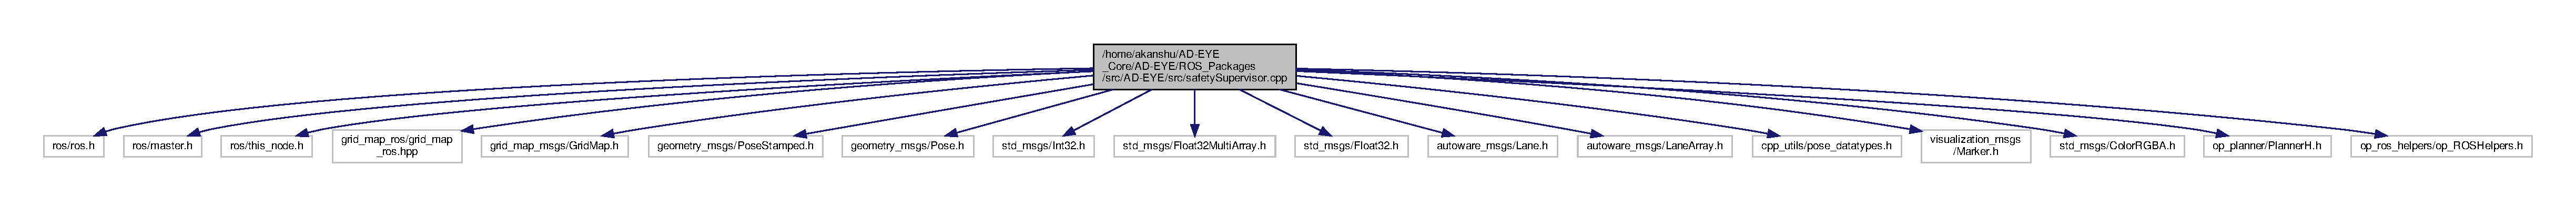
\includegraphics[width=350pt]{safetySupervisor_8cpp__incl}
\end{center}
\end{figure}
\subsection*{Classes}
\begin{DoxyCompactItemize}
\item 
class \hyperlink{classSafetySupervisor}{Safety\+Supervisor}
\begin{DoxyCompactList}\small\item\em The Safety Supervisor supervise the automated driving. \end{DoxyCompactList}\end{DoxyCompactItemize}
\subsection*{Functions}
\begin{DoxyCompactItemize}
\item 
int \hyperlink{safetySupervisor_8cpp_a3c04138a5bfe5d72780bb7e82a18e627}{main} (int argc, char $\ast$$\ast$argv)
\end{DoxyCompactItemize}


\subsection{Function Documentation}
\mbox{\Hypertarget{safetySupervisor_8cpp_a3c04138a5bfe5d72780bb7e82a18e627}\label{safetySupervisor_8cpp_a3c04138a5bfe5d72780bb7e82a18e627}} 
\index{safety\+Supervisor.\+cpp@{safety\+Supervisor.\+cpp}!main@{main}}
\index{main@{main}!safety\+Supervisor.\+cpp@{safety\+Supervisor.\+cpp}}
\subsubsection{\texorpdfstring{main()}{main()}}
{\footnotesize\ttfamily int main (\begin{DoxyParamCaption}\item[{int}]{argc,  }\item[{char $\ast$$\ast$}]{argv }\end{DoxyParamCaption})}


\hypertarget{safetySupervisor_8py}{}\section{/home/akanshu/\+A\+D-\/\+E\+Y\+E\+\_\+\+Core/\+A\+D-\/\+E\+Y\+E/\+R\+O\+S\+\_\+\+Packages/src/\+A\+D-\/\+E\+Y\+E/src/safety\+Supervisor.py File Reference}
\label{safetySupervisor_8py}\index{/home/akanshu/\+A\+D-\/\+E\+Y\+E\+\_\+\+Core/\+A\+D-\/\+E\+Y\+E/\+R\+O\+S\+\_\+\+Packages/src/\+A\+D-\/\+E\+Y\+E/src/safety\+Supervisor.\+py@{/home/akanshu/\+A\+D-\/\+E\+Y\+E\+\_\+\+Core/\+A\+D-\/\+E\+Y\+E/\+R\+O\+S\+\_\+\+Packages/src/\+A\+D-\/\+E\+Y\+E/src/safety\+Supervisor.\+py}}
\subsection*{Classes}
\begin{DoxyCompactItemize}
\item 
class \hyperlink{classsafetySupervisor_1_1safetySupervisor}{safety\+Supervisor.\+safety\+Supervisor}
\begin{DoxyCompactList}\small\item\em This is a class for evaluating the \char`\"{}safety of the Supervisor\char`\"{}. \end{DoxyCompactList}\end{DoxyCompactItemize}
\subsection*{Namespaces}
\begin{DoxyCompactItemize}
\item 
 \hyperlink{namespacesafetySupervisor}{safety\+Supervisor}
\end{DoxyCompactItemize}
\subsection*{Variables}
\begin{DoxyCompactItemize}
\item 
\hyperlink{namespacesafetySupervisor_ab9332624bdbffc606b516ac58d397f90}{safety\+Supervisor.\+anonymous}
\item 
\hyperlink{namespacesafetySupervisor_af6fe8549eb602b569a93fa71d153cc10}{safety\+Supervisor.\+sS} = safety\+Supervisor()
\end{DoxyCompactItemize}

\hypertarget{sender_8py}{}\section{/home/akanshu/\+A\+D-\/\+E\+Y\+E\+\_\+\+Core/\+A\+D-\/\+E\+Y\+E/\+R\+O\+S\+\_\+\+Packages/src/\+A\+D-\/\+E\+Y\+E/src/sender.py File Reference}
\label{sender_8py}\index{/home/akanshu/\+A\+D-\/\+E\+Y\+E\+\_\+\+Core/\+A\+D-\/\+E\+Y\+E/\+R\+O\+S\+\_\+\+Packages/src/\+A\+D-\/\+E\+Y\+E/src/sender.\+py@{/home/akanshu/\+A\+D-\/\+E\+Y\+E\+\_\+\+Core/\+A\+D-\/\+E\+Y\+E/\+R\+O\+S\+\_\+\+Packages/src/\+A\+D-\/\+E\+Y\+E/src/sender.\+py}}
\subsection*{Namespaces}
\begin{DoxyCompactItemize}
\item 
 \hyperlink{namespacesender}{sender}
\end{DoxyCompactItemize}
\subsection*{Functions}
\begin{DoxyCompactItemize}
\item 
def \hyperlink{namespacesender_a395e7bae8fd61526670d999891ecf5fd}{sender.\+mycallback1} (data)
\item 
def \hyperlink{namespacesender_a144bddc369cab38dc0793208e8928046}{sender.\+listener} ()
\end{DoxyCompactItemize}

\hypertarget{tracked__objects__adapter_8py}{}\section{/home/akanshu/\+A\+D-\/\+E\+Y\+E\+\_\+\+Core/\+A\+D-\/\+E\+Y\+E/\+R\+O\+S\+\_\+\+Packages/src/\+A\+D-\/\+E\+Y\+E/src/tracked\+\_\+objects\+\_\+adapter.py File Reference}
\label{tracked__objects__adapter_8py}\index{/home/akanshu/\+A\+D-\/\+E\+Y\+E\+\_\+\+Core/\+A\+D-\/\+E\+Y\+E/\+R\+O\+S\+\_\+\+Packages/src/\+A\+D-\/\+E\+Y\+E/src/tracked\+\_\+objects\+\_\+adapter.\+py@{/home/akanshu/\+A\+D-\/\+E\+Y\+E\+\_\+\+Core/\+A\+D-\/\+E\+Y\+E/\+R\+O\+S\+\_\+\+Packages/src/\+A\+D-\/\+E\+Y\+E/src/tracked\+\_\+objects\+\_\+adapter.\+py}}
\subsection*{Namespaces}
\begin{DoxyCompactItemize}
\item 
 \hyperlink{namespacetracked__objects__adapter}{tracked\+\_\+objects\+\_\+adapter}
\end{DoxyCompactItemize}
\subsection*{Functions}
\begin{DoxyCompactItemize}
\item 
def \hyperlink{namespacetracked__objects__adapter_aa9159f931fa00e5ccaf2ea118d9fab3d}{tracked\+\_\+objects\+\_\+adapter.\+mycallback1} (data)
\end{DoxyCompactItemize}
\subsection*{Variables}
\begin{DoxyCompactItemize}
\item 
bool \hyperlink{namespacetracked__objects__adapter_a174da94c280faf7a1cf732be6855739f}{tracked\+\_\+objects\+\_\+adapter.\+pos\+\_\+flag} = False
\item 
\hyperlink{namespacetracked__objects__adapter_acd6da79b4ebbc7777f1861371ef6bd2a}{tracked\+\_\+objects\+\_\+adapter.\+current\+\_\+pose} = Pose\+Stamped()
\item 
\hyperlink{namespacetracked__objects__adapter_a567640623bec81f5470b8ccabda3567a}{tracked\+\_\+objects\+\_\+adapter.\+trans} = list()
\item 
\hyperlink{namespacetracked__objects__adapter_a5cb9b213a87ca24a97729b3fba9a7733}{tracked\+\_\+objects\+\_\+adapter.\+rot} = list()
\item 
\hyperlink{namespacetracked__objects__adapter_af4a427c4003ca85ae020af7899fe1c20}{tracked\+\_\+objects\+\_\+adapter.\+anonymous}
\item 
\hyperlink{namespacetracked__objects__adapter_a11650b5ea8079756ceee7312396621b2}{tracked\+\_\+objects\+\_\+adapter.\+tflistener} = tf.\+Transform\+Listener()
\item 
\hyperlink{namespacetracked__objects__adapter_abd2ffc41d426e7fb5529885d7bafa9b5}{tracked\+\_\+objects\+\_\+adapter.\+rate} = rospy.\+Rate(10.\+0)
\end{DoxyCompactItemize}

%--- End generated contents ---

% Index
\backmatter
\newpage
\phantomsection
\clearemptydoublepage
\addcontentsline{toc}{chapter}{Index}
\printindex

\end{document}
